\documentclass[11pt]{article}
\usepackage[T1]{fontenc}
\usepackage[utf8]{inputenc}
\usepackage{lmodern,amsmath,amssymb,amsthm,mathtools,mathrsfs}
\input{glyphtounicode.tex}
\input{glyphtounicode-cmex.tex}
\pdfgentounicode=1
\usepackage[a4paper,margin=28mm]{geometry}
\usepackage{microtype,enumitem,booktabs,longtable,array,graphicx,xcolor}
\usepackage{tikz}
\usetikzlibrary{arrows.meta,calc,positioning,fit}
\usepackage{xurl}
\usepackage[colorlinks=true,linkcolor=blue!45!black,
  citecolor=blue!45!black,urlcolor=blue!45!black]{hyperref}
\usepackage{bookmark}
\usepackage[nameinlink,capitalise,noabbrev]{cleveref}
\makeatletter
\newcommand\SK@theorem@refstepcounter[2][]{%
  \Hy@theorem@refstepcounter{#2}%
  \@ifundefined{cref@#1@alias}%
    {\def\@tempa{#1}}%
    {\def\@tempa{\csname cref@#1@alias\endcsname}}%
  \protected@edef\cref@currentlabel{%
    \expandafter\cref@override@label@type
      \cref@currentlabel\@nil{\@tempa}}%
}
\@ifundefined{Hy@theorem@refstepcounter}
  {\PackageError{sk-cutoff}{Deferred theorem anchors are unavailable}
    {Check the installed hyperref version.}}
  {\patchcmd{\cref@thmoptarg}{\refstepcounter}{\SK@theorem@refstepcounter}
     {}{\PackageError{sk-cutoff}{Shared-counter theorem anchor patch failed}
       {Check the installed cleveref and hyperref versions.}}%
   \patchcmd{\cref@thmnoarg}{\refstepcounter}{\Hy@theorem@refstepcounter}
     {}{\PackageError{sk-cutoff}{Theorem anchor patch failed}
       {Check the installed cleveref and hyperref versions.}}}
\makeatother

\newtheorem{theorem}{Theorem}[section]
\newtheorem{proposition}[theorem]{Proposition}
\newtheorem{lemma}[theorem]{Lemma}
\newtheorem{corollary}[theorem]{Corollary}
\theoremstyle{definition}
\newtheorem{definition}[theorem]{Definition}
\newtheorem{assumption}[theorem]{Assumption}
\theoremstyle{remark}
\newtheorem{remark}[theorem]{Remark}
\newcommand{\E}{\mathbb E}
\renewcommand{\P}{\mathbb P}
\newcommand{\R}{\mathbb R}
\newcommand{\N}{\mathbb N}
\newcommand{\1}{\mathbf 1}
\DeclareMathOperator{\Var}{Var}
\DeclareMathOperator{\Cov}{Cov}
\DeclareMathOperator{\Ent}{Ent}
\DeclareMathOperator{\TV}{TV}
\DeclareMathOperator{\Tr}{Tr}
\DeclareMathOperator{\diag}{diag}
\DeclareMathOperator{\supp}{supp}
\DeclareMathOperator{\spec}{spec}
\newcommand{\op}{\mathrm{op}}
\newcommand{\HS}{\mathrm{HS}}
\newcommand{\dd}{\,\mathrm d}
\newcommand{\norm}[1]{\left\lVert #1\right\rVert}
\newcommand{\abs}[1]{\left\lvert #1\right\rvert}
\newcommand{\ip}[2]{\left\langle #1,#2\right\rangle}
\numberwithin{equation}{section}
\setlist{itemsep=2pt,topsep=5pt}
\setcounter{tocdepth}{2}
\hypersetup{
  pdfauthor={OpenAI},
  pdftitle={Cutoff throughout the high-temperature Sherrington--Kirkpatrick phase},
  pdfsubject={Glauber dynamics, cutoff, and an equilibrium spectral formula},
  pdfkeywords={Sherrington--Kirkpatrick model, Glauber dynamics, cutoff, high temperature}
}

\title{Cutoff throughout the high-temperature\\
  Sherrington--Kirkpatrick phase}
\author{OpenAI}
\date{September 24, 2026}
\begin{document}
\maketitle
\begin{abstract}
We prove worst-case total-variation cutoff for the zero-field Gaussian
Sherrington--Kirkpatrick heat-bath dynamics at every fixed inverse
temperature \(0\leq\beta<1\).
With rate-one refresh at each spin, the cutoff location is
\(\log n/(2\lambda(\beta))\) for a positive deterministic rate
\(\lambda(\beta)\). The location for uniformly chosen single-site
update attempts is \(n\) times as large. Convergence is in probability
over the disorder.
\end{abstract}
\tableofcontents
\section{Introduction}

We prove worst-start total-variation cutoff for single-site heat-bath
dynamics throughout the high-temperature phase of the zero-field
Gaussian Sherrington--Kirkpatrick model.  The cutoff location is
determined by an equilibrium gradient operator constructed in this
paper.  The distinction between equilibrium relaxation and worst-start
mixing is central: a positive spectral gap controls equilibrium
fluctuations, but a cutoff theorem must also identify when an arbitrary
initial configuration loses its remaining bias.

The Sherrington--Kirkpatrick model has random interactions of mixed
signs \cite{SK1975}.  These interactions make the required control of
nonequilibrium trajectories delicate even at high temperature.

Functional inequalities have provided quantitative high-temperature
control. The random-SK bounds in the following comparison hold with
probability tending to one over the disorder, at each fixed temperature
in the stated range.  Bauerschmidt and Bodineau~\cite{BB2019} proved a uniform
logarithmic Sobolev inequality for \(\beta<1/4\) with an unweighted
flip-gradient form.  Eldan, Koehler, and Zeitouni~\cite{EKZ2022}
obtained a heat-bath Poincar\'e inequality in that range.
Anari, Jain, Koehler, Pham, and Vuong~\cite{AJKPV2022} obtained
\(O(n\log n)\) mixing there, uniformly over external fields, through
entropic independence. Adhikari, Brennecke, Xu, and Yau~\cite{ABXY2024}
proved heat-bath gap estimates for mixed \(p\)-spin models at sufficiently
high temperature.
The localization framework of Chen and Eldan~\cite{CE2025} relates
entropy contraction to covariance estimates along tilted measures.
Anari, Koehler, and Vuong~\cite{AKV2024} extended
\(O(n\log n)\) Glauber mixing to a threshold approximately \(0.295\).
Wang~\cite{Wang2026} proved
\(O_\beta(n\log(n/\varepsilon))\) worst-start mixing for every fixed
\(\beta<1/2\), uniformly over external fields.
These mixing times count single-site update attempts.
Boban, Li, and Oveis Gharan~\cite{BLO2026} proved a positive unscaled
heat-bath gap in zero field for \(\beta<1/2+\varepsilon_0\), with a
universal \(\varepsilon_0\geq5\cdot10^{-5}\), yielding \(O_\beta(n^2)\) single-site update attempts at fixed
total-variation accuracy.
These results do not identify a cutoff location.

The companion article \cite{SKGap} proves a positive unscaled heat-bath
gap for every fixed \(\beta<1\) in the zero-field Gaussian model.
We record the precise imports in \Cref{sec:model} and prove the
additional arbitrary-law mean, path, and gradient estimates needed for
cutoff here.  They identify the leading location through a deterministic
equilibrium spectral construction.  The resulting rate is implicit.
The appendices give an independent proof of the cutoff ratio for
\(\beta<1/2\), with its own scalar certificate and auxiliary estimates
uniform over external fields and interaction scalings.  Those stronger auxiliary uniformities
are confined to the restricted-temperature method.

\subsection{The result}

For \(\Omega_n=\{-1,1\}^n\), let \(J\) be symmetric with zero diagonal
and independent \(J_{ij}\sim N(0,\beta^2/n)\) for \(i<j\). The Gibbs law is
\[
 \mu_J(x)=Z_J^{-1}\exp\!\left(\frac12x^{\mathsf T}Jx\right).
\]
This normalization puts the equilibrium high-temperature boundary at
\(\beta=1\): the normalized mean pressure \(n^{-1}\E\log Z_J\)
tends to \(\log2+\beta^2/4\) for \(\beta<1\)
\cite[Proposition~2.1]{ALR1987}. For \(\beta>1\), Guerra's
variational bound~\cite{Guerra2003} gives a limit superior strictly
smaller than \(\log2+\beta^2/4\).

At each spin a rate-one clock replaces that spin by a sample from its
conditional law under \(\mu_J\), given the other spins. Write \(S_t\)
for this transition kernel and \(P\) for one uniformly chosen single-site
refresh attempt; attempts that retain the old spin are included.
At fixed disorder put
\[
 d_n(t)=\max_x\|S_t(x,\cdot)-\mu_J\|_{\TV},\qquad
 d_n^{\rm disc}(k)=\max_x\|P^k(x,\cdot)-\mu_J\|_{\TV},
\]
where \(\|\nu-\mu\|_{\TV}=\frac12\sum_x|\nu(x)-\mu(x)|\).
We abbreviate \(\mu_J\) to \(\mu\). Section~\ref{sec:model} develops the
half-difference and Dirichlet-form conventions used in the proof.

\begin{theorem}
\label{thm:main}
For every fixed \(0\leq\beta<1\), there is a deterministic
\(\lambda(\beta)>0\) such that, with
\[
 t_n=\frac{\log n}{2\lambda(\beta)},
\]
for every \(\epsilon\in(0,1)\),
\begin{align*}
 d_n((1-\epsilon)t_n)&\longrightarrow1,
 &
 d_n((1+\epsilon)t_n)&\longrightarrow0,\\
 d_n^{\rm disc}(\lfloor(1-\epsilon)nt_n\rfloor)&\longrightarrow1,
 &
 d_n^{\rm disc}(\lceil(1+\epsilon)nt_n\rceil)&\longrightarrow0.
\end{align*}
All convergences are in probability over the disorder.
For \(\beta=0\), \(\lambda(0)=1\).
For \(0<\beta<1\), \(\lambda(\beta)\) is the equilibrium-operator
constant defined in \eqref{eq:exact-lambda}; it satisfies
\[
 0<\lambda(\beta)\leq(1-\beta)^2.
\]
\end{theorem}

The theorem answers the high-temperature cutoff question in the
zero-field Gaussian setting.  The temperature is fixed before the
dimension tends to infinity.  We do not address a temperature
approaching \(1\) with \(n\), external fields, or a cutoff window.

\subsection{The rate and the gradient mechanism}

A half-difference measures an observable's sensitivity to one spin:
\[
 d_i f(x)=\frac{f(x^{i,+})-f(x^{i,-})}{2},
 \qquad df=(d_1f,\ldots,d_nf),
\]
where \(x^{i,\pm}\) is obtained from \(x\) by fixing spin \(i\) to
\(\pm1\). We call a vector field of the form \(df\) an exact gradient.
Differentiating heat flow gives a vector semigroup \(K_t\) satisfying
\[
 dS_tf=K_tdf.
\]
Its finite-dimensional generator is derived in
Section~\ref{sec:gradient-path}. Thus decay under \(K_t\) controls
how strongly a smoothed observable can still distinguish its starting
configuration.

The scale relevant to total variation is visible in the elementary bound
\[
 \max_x g(x)-\min_x g(x)
 \le 2\sqrt n\,\sup_x\|dg(x)\|.
\]
For the upper bound, the proof makes the gradient of \(S_tf\) smaller
than \(n^{-1/2}\), uniformly for \(|f|\le1\), by combining gradient
propagation with a late-time energy bound. For the lower bound, it finds
an observable with bounded fluctuations and a mean bias that decays at
any rate just above \(\lambda\), from an initial size arbitrarily close
to \(\sqrt n\) on a logarithmic scale. These two thresholds explain
the location \(\log n/(2\lambda)\).

Two equilibrium rates can govern this decay. First, start the chain in
\(\mu\) and consider its normalized spin autocorrelation
\[
 C_n(t)=\frac1n\E_\mu[X_0^{\mathsf T}X_t].
\]
Section~\ref{sec:row-spin} proves convergence to
\(C(t)=\int e^{-ut}\rho(\dd u)\) for a deterministic positive
probability measure \(\rho\). Its lower support edge is
\(\lambda_{\rm sp}=\inf\supp\rho>0\).
This rate describes the slowest part detected by the limiting averaged
spin correlation.

The second rate is obtained by retaining more equilibrium observables.
A finite calculation starts with the spin vector and fixed independent
site seeds, and uses multiplication by \(J\), linear combinations,
and smooth componentwise functions. For example, the local-field vector
\(Jx\) and the conditional-mean vector \(\tanh(Jx)\) are such
calculations. After normalization by \(n^{-1/2}\), their limiting
equilibrium overlaps define a deterministic Hilbert space of
\emph{visible} vectors. A sequence of endpoint vectors is \emph{hidden}
when its contractions with every fixed such calculation vanish in
square mean.
Section~\ref{sec:gaussian-calculus} constructs this space and its
conditional path predictions.

For exact gradients, the natural equilibrium energy uses the conditional
spin variances \(v_i(x)=1-\tanh^2((Jx)_i)\):
\[
 \|p\|_v^2=\E_\mu\sum_i v_i p_i^2.
\]
Section~\ref{sec:exact} constructs an invariant family of equilibrium
test gradients from the finite calculations and completes it in this
weighted norm. The resulting space \(\mathcal X_v\) contains every
weighted-visible limit of exact gradients relevant to the proof.
On it, the limiting \(K_t\) is self-adjoint; write
\(\mathcal A_v=-{\rm gen}(K|_{\mathcal X_v})\). This is a preview
of the precise test-potential construction in
Definition~\ref{def:exact-spaces} and its saturation result. The rate is
\[
 \lambda=\min\{\lambda_{\rm sp},\inf\spec(\mathcal A_v)\},
 \qquad
 0<\lambda\le\lambda_{\rm sp}\le(1-\beta)^2.
\]
All these objects are constructed from equilibrium quantities at fixed
times: dimension tends to infinity before any subsequent large-time or
spectral-edge limit. If the second rate is smaller, the proof isolates a
finite-dimensional family of slower observables and uses it for the
lower bound. The formula does not identify \(\lambda\) with the upper
bound \((1-\beta)^2\).

\subsection{Main ideas}

The main difficulty is to make these equilibrium decay mechanisms
control every starting configuration for logarithmically long times.
The proof establishes fixed-time comparisons first, then makes a single
sufficiently long block uniform before iterating it.

\paragraph{Bringing arbitrary starts into the comparison regime.}
We strengthen the stable-field residual argument underlying the companion
gap theorem to control the mean under an arbitrary change of law. The
change in mean is bounded by \(C(1+\sqrt D)\), where \(D\) is the
Dirichlet energy of the square-root density. Transport through a two-stage Gaussian observation
then gives entropy control and the fixed-time heat-kernel estimate
\[
 \frac1n\log\left\|\frac{S_d(x,\cdot)}{\mu}\right\|_\infty
 \le C e^{-c d^{2/3}}.
\]
Here \(d\) is fixed before \(n\to\infty\). Choosing a sufficiently
long fixed burn-in makes this density cost small enough for exponentially
reliable equilibrium comparisons to survive the changed law. The
observation argument also supplies the posterior and cavity gaps used
later; the zero-field gap alone would not supply them.

\paragraph{Averaging the hidden part from both endpoints.}
The path expansion of \(K_t\) involves products of \(J\) and diagonal
labels depending on observed spin states. We compare each label with
its conditional prediction from the initial or terminal state. A
conditional-covariance argument shows that terms containing both an
initially centered label and a later terminally centered label vanish
when tested against a hidden initial vector and an exact terminal
gradient. This leaves strings predicted from their two endpoints, with
at most one actual path label between them.

Two estimates make this averaging useful. A projected row likelihood
has subexponential moments in the interval length, while the spin
spectral measure supplies summable positive path weights at every rate
below \(\lambda_{\rm sp}\). Their combination proves hidden-gradient
decay at that edge. To justify the covariance cancellation for multitime
labels, we propagate mixed differences through conditional evolution and
copied observation states. The resulting directed networks retain the
derivative continuing to the terminal gradient. This is the role of the
derivative machinery in Sections~\ref{sec:gradient-path} and
\ref{sec:gaussian-calculus}. Its operator estimates also retain rare
coordinate types, whose small spatial frequency need not make their
operator action small.

\paragraph{Recovering the visible exact part.}
Projecting a nonstationary gradient onto the visible calculations gives
random scalar coefficients. Transport acts on the deterministic vector
directions by \(K_t\) and on these coefficients by conditional
expectation. The projection does not immediately preserve the identities
that characterize a gradient. Reverse entropy estimates and strong
control of weighted curl restore those identities; a second observation
argument then bounds the distance to actual gradients. This places the
visible projection in \(\mathcal X_v\) without differentiating its
possibly irregular coefficients. The hidden bound further shows that
any visible spectrum below \(\lambda_{\rm sp}\) consists of isolated
modes of finite multiplicity.

\paragraph{From a fixed block to the two cutoff bounds.}
The hidden and visible estimates give contraction on one long fixed
block. Strict contraction slack and normalization make this bound uniform
over all starts and tests, with an inverse-polynomial additive error;
iteration therefore reaches logarithmic times without assuming a
quantitative rate for a fixed-time limit. A late-time martingale-energy
estimate completes the upper bound. For the lower bound, spin correlation
provides the distinguishing observable when
\(\lambda=\lambda_{\rm sp}\). If a slower visible mode determines
\(\lambda\), an additional block estimate aligns both the mean and
fluctuations of its random coefficient. A small perturbation of the
initial law then creates a detectable slow bias, and convexity selects
a deterministic starting configuration with at least the same
separation from equilibrium.

\subsection{Organization and dependencies}

Section~\ref{sec:model} fixes the normalizations and companion inputs,
and states the finite-chain concentration and clock estimates.
Section~\ref{sec:static} proves the arbitrary-law and observation bounds.
Sections~\ref{sec:gradient-path} and~\ref{sec:gaussian-calculus} develop
the gradient evolution, conditional derivatives, and Gaussian path
calculus. Section~\ref{sec:row-spin} treats the projected row likelihood
and the spin spectral measure; Section~\ref{sec:hidden} uses them to
prove hidden propagation. Section~\ref{sec:exact} constructs the visible
exact operator and isolates its slower spectrum. Section~\ref{sec:cutoff}
assembles the uniform blocks and proves cutoff for both clocks.
Appendices~\ref{sec:rcut-introduction}--\ref{rcut:sec:scalar-certificate}
give the independent restricted-temperature argument and its scalar
certificate. Appendix~\ref{app:clock-comparison} proves the common
clock lemma. Figure~\ref{fig:proof-dependencies} records the principal
dependencies.

\begin{figure}[htbp]
\centering
\begin{tikzpicture}[
  box/.style={draw=black!60,rounded corners=2pt,fill=black!3,
    text width=5.15cm,align=center,inner sep=7pt,font=\small},
  arrow/.style={-{Stealth[length=2.2mm]},draw=black!65,line width=.6pt},
  node distance=11mm and 13mm]
 \node[box] (static) {Observation and entropy (\S\ref{sec:static})\\
   Density and posterior control};
 \node[box,right=of static] (paths) {Finite-time Gaussian calculus\\(\S\S\ref{sec:gradient-path}--\ref{sec:gaussian-calculus})\\
   Conditional predictors\\and matrix words};
 \node[box,below=of static] (row) {Projected row moments (\S\ref{sec:row-spin})\\
   Spin spectral edge \(\lambda_{\rm sp}\)};
 \node[box,below=of paths] (exact) {Weighted gradient exactness (\S\ref{sec:exact})\\
   The visible sector \(\mathcal X_v\)};
 \node[box,below=of row] (hidden) {Two-ended path averaging (\S\ref{sec:hidden})\\
   Hidden decay at \(\lambda_{\rm sp}\)};
 \node[box,below=of exact] (spectral) {Spectral isolation (\S\ref{sec:exact})\\
   Slower visible eigenmodes};
 \coordinate (middle) at ($(hidden.south)!.5!(spectral.south)$);
 \node[box,below=14mm of middle,
   text width=8cm] (cutoff)
   {Uniform fixed-block estimates (\S\ref{sec:cutoff})\\
    Upper cutoff and the two spectral lower bounds};
 \draw[arrow] (static) -- (row);
 \draw[arrow] (paths) -- (row);
 \draw[arrow] (paths) -- (exact);
 \draw[arrow] (static) -- (exact);
 \draw[arrow] (row) -- (hidden);
 \draw[arrow] (exact) -- (spectral);
 \draw[arrow] (hidden) -- (spectral);
 \draw[arrow] (hidden) -- (cutoff);
 \draw[arrow] (spectral) -- (cutoff);
\end{tikzpicture}

\caption{The principal estimates and their use in the cutoff proof.
All limiting comparisons precede the iteration over logarithmically
many fixed-time blocks. The stationary gap is an input; the
reweighting, averaging, and exactness arguments are proved here.}
\label{fig:proof-dependencies}
\end{figure}

\section{The model, normalization, and imported estimates}
\label{sec:model}

We first fix the relation between the two update clocks, the discrete
half-differences, and the heat-bath Dirichlet form.  We then state the
fixed-temperature gap that the proof imports and the two finite-chain
estimates used to control fluctuations and change clocks. We prove the
jump-moment estimate here and the longer clock comparison in
Appendix~\ref{app:clock-comparison}. Both estimates use their stated
finite-chain hypotheses and have no high-temperature restriction.

\subsection{Two clocks and the Dirichlet form}

Let \(\Omega_n=\{-1,1\}^n\).  Independently for \(i<j\), choose
\(J_{ij}\sim N(0,\beta^2/n)\), set \(J_{ji}=J_{ij}\) and \(J_{ii}=0\), and put
\[
 \mu_J(x)=Z_J^{-1}\exp\!\left(\frac12x^{\mathsf T}Jx\right).
\]
The inverse temperature \(\beta\) is fixed as \(n\) tends to infinity.
We suppress \(J\) from \(\mu\) and the transition kernels when this
does not cause confusion.
For \(x\in\Omega_n\), write \(x^i\) for the configuration with spin \(i\)
reversed, and write \(x^{i,+}\) and \(x^{i,-}\) for the configurations
obtained by fixing that spin to \(+1\) and \(-1\), respectively.
Define the half-difference
\[
 d_i f(x)=\frac{f(x^{i,+})-f(x^{i,-})}{2}.
\]
This derivative is independent of \(x_i\).  Writing the conditional
mean, conditional variance, and twice the flip rate as
\[
 m_i(x)=\tanh((Jx)_i),\qquad
 v_i(x)=1-m_i(x)^2,\qquad
 w_i(x)=1-x_i m_i(x),
\]
the generator with one refresh attempt per spin per unit time is
\begin{equation}
 Lf(x)=\sum_{i=1}^n (m_i(x)-x_i)d_i f(x)
      =\sum_{i=1}^n\frac{w_i(x)}2\bigl(f(x^i)-f(x)\bigr).
 \label{eq:model-generator}
\end{equation}
Its semigroup is \(S_t=e^{tL}\).
The kernel \(P\) of one uniformly chosen single-site refresh attempt
therefore satisfies \(L=n(P-I)\).
Both clocks include attempts which leave the configuration unchanged.

We define the unscaled form for any full-support law \(Q\) on the cube
by conditional covariance:
\[
 \mathcal E_Q(f,g)
   =\sum_i \E_Q\Cov_Q(f,g\mid X_{-i}),\qquad
 \mathcal E_Q(f)=\mathcal E_Q(f,f).
\]
When \(Q\) is a Gibbs law with the above interaction and an external
field, let \(v_i\) denote the conditional variance for that law.  Then
\begin{equation}
 \mathcal E_Q(f,g)=\E_Q\sum_i v_i\,d_i f\,d_i g.
 \label{eq:model-dirichlet}
\end{equation}
In particular,
\[
 -\E_\mu[fLg]=\mathcal E_\mu(f,g),\qquad
 \E_\mu[w_i\mid X_{-i}]=v_i,\qquad
 \E_\mu[w_i^2\mid X_{-i}]=v_i.
\]
The last two identities follow by conditioning on \(X_{-i}\) and
averaging a sign with mean \(m_i\).  They explain the two weights:
\(w_i\) occurs in the jump rates and hence in pointwise quadratic
variation, while conditioning converts the stationary energy to the
\(v_i\)-weighted form.  We will make this conversion only inside the
corresponding stationary expectation.

Differentiating the generator later will require the exact product
rule, including its quadratic correction, and the commutation identities
\begin{align}
 d_i(fg)&=f\,d_i g+g\,d_i f-2x_i\,d_i f\,d_i g,
 \label{eq:model-product}\\
 d_i d_jf&=d_jd_if,\qquad d_i^2f=0.
 \label{eq:model-commute}
\end{align}
The zero-field symmetry gives \(\E_\mu X=0\), which will fix the
centering of equilibrium spin observables.  All vector norms are
unnormalized Euclidean norms.
Matrix norms are operator or Hilbert--Schmidt norms unless a normalized
trace \(n^{-1}\Tr\) is written explicitly.
We use \(D_a=\diag(a_1,\ldots,a_n)\).

For a probability density \(g\) relative to \(Q\), write
\[
 \Ent_Q(g)=\E_Q[g\log g],\qquad \E_Qg=1.
\]
For an arbitrary nonnegative \(g\), the homogeneous convention is
\(\Ent_Q(g)=\E_Q[g\log(g/\E_Qg)]\).
Total variation is
\[
 \norm{\nu-\mu}_{\TV}
   =\frac12\sum_{x\in\Omega_n}\abs{\nu(x)-\mu(x)}.
\]
Set
\[
 d_n(t)=\max_{x\in\Omega_n}\norm{S_t(x,\cdot)-\mu}_{\TV},
 \qquad
 d_n^{\rm disc}(k)=\max_{x\in\Omega_n}\norm{P^k(x,\cdot)-\mu}_{\TV}.
\]
Probabilities without a chain subscript refer to the disorder when
the event is a statement about \(J\); conditional path probabilities
are always taken with \(J\) fixed.

\subsection{The spectral-gap input}

The equilibrium input is an all-functions Poincar\'e inequality at a
fixed subcritical temperature.  Its form is the unscaled form just
defined, so its constant controls rate-one-per-site dynamics.

\begin{theorem}[High-temperature gap {\cite[Theorem~1.1]{SKGap}}]
\label{thm:input-gap}
For every fixed \(0<\beta<1\), there is \(\gamma_\beta>0\) such that,
with probability tending to one over \(J\),
\[
 \Var_\mu(f)\leq\gamma_\beta^{-1}\mathcal E_\mu(f)
 \quad\text{for every real function }f\text{ on }\Omega_n.
\]
\end{theorem}

The reference proves this for zero field and Gaussian off-diagonal
variance \(\beta^2/n\), with
\(\mathcal E_\mu=\sum_i\E_\mu\Var(\,\cdot\,\mid X_{-i})\).
Its discrete-time gap is consequently the unscaled gap divided by \(n\).
The same companion supplies deterministic Gaussian-matrix diagnostics
and stable-field residual estimates.  Section~\ref{sec:static} states
those hypotheses before using them.  The arbitrary-law mean estimate in
\Cref{lem:stat-mean} and the simultaneous posterior and cavity gaps in
\Cref{prop:stat-posterior-gap} require additional arguments, which we
supply there.  In particular, \Cref{thm:input-gap} is a zero-field
statement and does not supply a uniform gap at arbitrary external fields.

For any fixed collection of comparisons, intersect the gap event with
the finitely many matrix-diagnostic events those comparisons require.
On the resulting good-disorder event a fixed operator bound
\(\norm J\leq C_\beta\) also holds.
It implies
\begin{equation}
 \min_{x\in\Omega_n}\mu(x)\geq
 \exp\bigl(-(\log2+C_\beta)n\bigr),
 \label{eq:model-minmass}
\end{equation}
because \(\abs{x^{\mathsf T}Jx}/2\leq C_\beta n/2\).
Later arguments selecting countably many comparison tests use a
diagonal sequence of such finite good events; the required
uniformity is stated explicitly in \Cref{thm:path-calculus,prop:cutoff-block}.

\subsection{Two reusable consequences for finite chains}

We now leave the random-matrix input aside.  The first estimate turns a
pointwise gradient bound into exponential moments of a terminal observable.
The second compares averages under shifted Poisson clocks with averages
under a binomial clock.  Both estimates also enter the independent restricted-temperature argument
in the appendices; their proofs use only the finite-chain hypotheses.

\begin{lemma}[Jump exponential moments]
\label{lem:input-mgf}
Fix \(d\geq0\) and \(f:\Omega_n\to\R\).
Suppose a bounded measurable function \(b:[0,d]\to[0,\infty)\) satisfies
\[
 \sup_x\norm{dS_r f(x)}^2\leq b(r)\quad(0\leq r\leq d).
\]
Put \(B=\sup b\) and \(I=\int_0^d b(r)\dd r\).  Then, for every
\(\theta\in\R\) and every starting state \(x\),
\begin{equation}
 \E_x\exp\!\left(\theta(f(X_d)-S_df(x))\right)
 \leq \exp\!\left(2\theta^2 e^{2\abs\theta\sqrt B}I\right).
 \label{eq:model-jump-mgf}
\end{equation}
In particular, \(\Var_x(f(X_d))\leq4I\).
\end{lemma}

\begin{proof}
Use the backward martingale \(F(s,X_s)=S_{d-s}f(X_s)\), whose initial
value is \(S_df(x)\) and terminal value is \(f(X_d)\).  A spin flip
has increment \(-2x_i d_iF\), of magnitude at most
\(2\sqrt{b(d-s)}\).  Its instantaneous sum of squared jump sizes
times rates is
\[
 \sum_i\frac{w_i}{2}(2d_iF)^2\leq4b(d-s).
\]
The backward equation cancels the linear part of the exponential
drift.  The remaining jump compensator is controlled by the preceding
square-jump bound and \(e^z-1-z\leq z^2e^{\abs z}/2\).  Integrating the
resulting drift inequality and dividing by \(e^{\theta S_df(x)}\)
gives \eqref{eq:model-jump-mgf}.  Expansion at \(\theta=0\) gives the
variance assertion.  This argument used the flip-rate bound and the
assumed gradient bound; it used no restriction on the temperature.
\end{proof}

The comparison between lazy discrete clocks and continuous semigroups
follows the shifted Poisson and binomial method of Chen and
Saloff-Coste~\cite[Theorem~1.1 and Lemmas~3.1--3.2]{ChenSaloffCoste2013}.
We give the bounded-array version needed for uniformity in the disorder.
\begin{lemma}[Clock comparison]
\label{lem:input-clock}
Fix $q\in(0,1)$, let $M_n\in\N$ tend to infinity, and let
$(a_{n,j})_{j\ge0}$ be real arrays satisfying
$\sup_{n,j}|a_{n,j}|\le B<\infty$.  Suppose that for every fixed
$y\in\R$,
\begin{equation}
 \E\bigl[a_{n,N_{n,y}}\bigr]\longrightarrow0,
 \qquad
 N_{n,y}\sim\operatorname{Poisson}
                   (q M_n+y\sqrt{M_n}).
 \label{eq:inputclock-poisson-hypothesis}
\end{equation}
The mean in this display is positive for all sufficiently large $n$.
If $B_n\sim\operatorname{Binomial}(M_n,q)$, then
$\E[a_{n,B_n}]\to0$.
The conclusion is uniform over an additional family of arrays and
values of $M_n$ when their bounds and the convergences in
Equation~\eqref{eq:inputclock-poisson-hypothesis} are uniform and $M_n$
tends uniformly to infinity.
\end{lemma}

The proof appears in Appendix~\ref{app:clock-comparison}. It first
approximates the two rescaled clocks by Gaussian densities, then
approximates the narrower Gaussian by a finite signed sum of translates
of the wider one. Fixing that sum before testing the arrays gives the
stated uniformity.


\subsection{The independent case}

The gap input assumes $\beta>0$.  At $\beta=0$, independence gives
the continuous-time cutoff directly, with rate equal to one.

\begin{proposition}
\label{prop:model-independent}
At \(\beta=0\), the continuous-time dynamics has cutoff at
\(\tfrac12\log n\).
\end{proposition}

\begin{proof}
For the upper bound, use the full density relative to equilibrium.
Starting from \(x\), the spins at time \(t\) are independent with
means \(e^{-t}x_i\).  Against uniform measure,
\[
 1+\chi^2(S_t(x,\cdot),\mu)=(1+e^{-2t})^n.
\]
Thus total variation tends to zero uniformly in \(x\) at
\(t=(1+\epsilon)\log n/2\).
For the lower bound, a single statistic suffices.  From the all-plus
state, the normalized sum
\(n^{-1/2}\sum_iX_i\) has mean \(\sqrt n\,e^{-t}\)
and variance at most one; at equilibrium its mean is zero
and its variance is one.
At \(t=(1-\epsilon)\log n/2\), the mean tends to infinity.
Chebyshev's inequality gives total variation tending to one.
\end{proof}

Henceforth \(0<\beta<1\).
The discrete independent case follows from the same clock comparison
used at the end of the paper.

\section{Static estimates and Gaussian observation}\label{sec:static}
\providecommand{\sech}{\operatorname{sech}}

Our goal is a uniform heat-kernel bound whose logarithm, divided by $n$,
can be made small by choosing a long but fixed time.  We obtain it in four
steps: control the mean under an arbitrary change of law; transport that
control along a Gaussian observation with simultaneous posterior and cavity
gaps; bound entropy at the product endpoint; and convert the entropy bound
to a semigroup norm estimate.  The first step strengthens the stable-field
estimates of \cite{SKGap}.  The observation step uses
the stochastic-localization method of Eldan~\cite{Eldan2013}, its
Gaussian-channel formulation by El Alaoui and Montanari~\cite{ElAlaouiMontanari2021},
and the localization-annealing framework of Chen and Eldan~\cite{CE2025}.
The stopped, changed-law estimates and simultaneous cavity conclusions
required here are proved below. Throughout
this section constants may depend on the fixed $\beta<1$.  They never depend
on the probability measure being compared with equilibrium.

The cost of changing a strictly positive cube law $P$ to a probability
$Q$ will be measured by its square-root Dirichlet energy and relative
entropy.  Set
\[
 D_P(Q)=\mathcal E_P\bigl(\sqrt{Q/P}\bigr),\qquad
 H_P(Q)=\sum_x Q(x)\log\frac{Q(x)}{P(x)}.
\]
The energy lies in $[0,n]$; values at zeros of $Q$ are defined by
continuity.  To see how it controls the change in a single conditional
spin law, write $P_i,Q_i$ for the conditional laws of spin $i$ given
all other spins.  Expanding the conditional variance gives
\begin{equation}\label{eq:stat-affinity}
 D_P(Q)=\sum_i\E_{Q_{-i}}\left[
 1-\left(\sum_{s=\pm1}\sqrt{P_i(s)Q_i(s)}\right)^2\right].
\end{equation}
Conditionals on a $Q_{-i}$-null configuration can be assigned arbitrarily.
For two probabilities $p,q$, Cauchy--Schwarz applied to
$(\sqrt p-\sqrt q)(\sqrt p+\sqrt q)$ gives
$\TV(p,q)^2\le1-(\sum\sqrt{pq})^2$.  Hence, if
$\bar m_i=\E_Q[x_i\mid x_{-i}]$ and
$m_i^P=\E_P[x_i\mid x_{-i}]$, then
\begin{equation}\label{eq:stat-conditional-means}
 \E_Q\sum_i(\bar m_i-m_i^P)^2\le4D_P(Q).
\end{equation}

\subsection{A stable field controls means under an arbitrary law}

We begin with the deterministic hypotheses under which the mean estimate
will hold.  These hypotheses come from \cite{SKGap}; the arbitrary-law
conclusion will be proved here.  For a symmetric interaction matrix $M$
with zero diagonal,
a parameter $0<j<1$, and a field $h$, put
\[
 m(y)=\tanh y,\qquad b(y)=\frac1n\sum_i\sech^2 y_i,
 \qquad V(y)=\diag(\sech^2 y_i),
\]
and, for a nonnegative diagonal matrix $A$, write
\begin{align}
 F_{M,h}(y)&=y-h+\{j b(y)I-M\}m(y),\label{eq:stat-field-map}\\
 \mathsf H_M(y,A)
 &=I+A^{1/2}\left(jb(y)I-M-\frac{2j}{n}
                 m(y)m(y)^{\mathsf T}\right)A^{1/2}.
 \label{eq:stat-field-hessian}
\end{align}
The stability hypothesis is a uniform implication over a small-residual
region and nearby diagonals.  More precisely, the field has fixed positive
margins $\rho_0,\epsilon_A,\kappa$ and $a_+>1$, with $j a_+^2<1$, such that
\begin{equation}\label{eq:stat-stability}
 \left.
 \begin{gathered}
 \norm{F_{M,h}(y)}\le\rho_0\sqrt n,\quad 0\le A\le a_+I,\\
 \norm{A-V(y)}_{\HS}\le\epsilon_A\sqrt n
 \end{gathered}\right\}
 \quad\Longrightarrow\quad \mathsf H_M(y,A)\succeq\kappa I.
\end{equation}
We also require the finite-word estimates of \cite[Lemma~3.1]{SKGap}.
Fix a length bound $L$, a diagonal norm bound $M_0$, and an inverse margin
$c_0>0$. A word $W$ is an ordered product of at most $L$ factors, each
either a real diagonal matrix of norm at most $M_0$, a copy of $M$, or
the following inverse, which may occur at most once:
\[
 K_A=(I-AM+j\chi_AA)^{-1},\qquad \chi_A=n^{-1}\Tr A,
 \qquad 0\le A\le a_+I.
\]
Words containing $K_A$ are considered only when
\[
 I+j\chi_AA-A^{1/2}MA^{1/2}\succeq c_0I.
\]
To define the diagonal prediction $\mathsf P(W)$ for a word without an
inverse, sum over complete noncrossing pairings of its occurrences of
$M$. Remove each innermost pair by
$MDM\mapsto j n^{-1}\Tr(D)I$ and combine adjacent diagonals. An odd number
of copies of $M$ gives zero prediction; a word with no $M$ predicts itself.
For an inverse factor, apply this rule coefficientwise to
$(I-zAM+z^2j\chi_AA)^{-1}$ expanded formally at $z=0$, and then set $z=1$.
The cited lemma shows that the resulting prediction is a polynomial in $z$.
The required bounds are
\begin{equation}\label{eq:stat-word-diagnostics}
 \norm W\le C_{\rm w},\qquad
 \left(\sum_{a\ne b}|W_{ab}|^4\right)^{1/4}\le C_{\rm w},\qquad
 \norm{\diag(W-\mathsf P(W))}_2\le C_{\rm w}.
\end{equation}
The entrywise and diagonal norms are unnormalized. These bounds hold
simultaneously in all the allowed diagonal choices; $C_{\rm w}$ is
independent of $n$. We refer to them, together with $\norm M\le K$, as
the deterministic diagnostics. The construction below chooses a sufficiently
large finite $L$ and fixed coefficient bounds before $n$ tends to infinity.
Constants in the mean estimate may depend on these bounds and the fixed
stability and inverse margins.

\begin{lemma}[Arbitrary-law mean bound]\label{lem:stat-mean}
Suppose $P(x)$ is proportional to
$\exp(x^{\mathsf T}Mx/2+h^{\mathsf T}x)$ and satisfies the deterministic
diagnostics and \Cref{eq:stat-stability}.  There is a constant $C$, uniform
over these fields, matrices, and dimensions, such that every probability
$Q$ on the cube satisfies
\begin{equation}\label{eq:stat-mean}
 \norm{\E_Qx-\E_Px}\le C\bigl(1+\sqrt{D_P(Q)}\bigr).
\end{equation}
The required diagnostic length is finite and depends only on the fixed
stability margins and the bounds in the construction.
\end{lemma}

\begin{proof}
We first extend the weak residual identity to expectations under $Q$,
then use first moments to select two consecutive small residuals, and
finally compare the selected iterate with the stable root.  The
deterministic differentiation bounds are supplied by
\cite[Lemmas~5.7, 6.1, 6.3, and~6.4]{SKGap}.  The conclusion
\Cref{eq:stat-mean}, including its square-root dependence on the energy,
is the additional assertion proved in this argument.

\emph{Residual identities under the changed law.}

The recursion uses Onsager corrections, as in Bolthausen's TAP
iteration~\cite{Bolthausen2014}. Post-iteration Gaussian comparison
and local convexity are studied by Celentano~\cite{Celentano2024}; neither
result substitutes for the buffered residual estimates used here.
Define the primary fields by
\[
 \begin{gathered}
 m^0=x,\quad b_0=0,\quad h^1=h+Mx,\quad
 m^l=\tanh h^l,\\
 b_l=n^{-1}\sum_i(1-(m_i^l)^2),\qquad
 h^{l+1}=h+Mm^l-jb_lm^{l-1},
 \end{gathered}
\]
and put $R_l=m^{l-1}-m^l$.  At any fixed depth the derivative matrices of
$h^l,m^l$ have bounded operator norm and
$\norm{db_l}\le C_l n^{-1/2}$.  The small-vector constructions in \cite[Definition~6.2]{SKGap} start with
seeds of bounded Euclidean norm that may depend on $M,h$ but are
independent of the spin $x$.
Their sources are finite sums of smooth site coefficients times seeds
or earlier auxiliary fields, and are linear in those auxiliary arguments.
The coefficients and their derivatives
through every fixed order used in the construction are uniformly bounded.
Scalar parameters $\theta$ satisfy
$\sup_x(|\theta(x)|+\norm{d\theta(x)})\le C$; they may include the averages
$b_l$. A source $U$ is admissible from level $p$ when every explicit
primary field in its site coefficients has index at least $p$.
In particular, the seed $(1,\ldots,1)/\sqrt n$ permits the source
$m^l/\sqrt n$ at level $l$.
An ordinary construction starts with an empty auxiliary list.
At stage $r$, write $w^r=U$ for the new source and $y^r$ for the
output of the operation below; the auxiliary sum runs over earlier
pairs $(w^a,y^a)$, $a<r$.  The formal partial $\partial_lU_i$
differentiates the explicit primary-field argument $h_i^l$, holding
the seeds, scalar parameters (including the averages $b_l$), and
auxiliary arguments fixed.  The partial $\partial_{y^a}U_i$
differentiates the linear argument $y_i^a$ with its coefficient
held fixed.  A partial in an absent argument is zero.
The associated auxiliary operation is
\begin{equation}\label{eq:stat-auxiliary}
 U\longmapsto MU-j\sum_l\alpha_lm^{l-1}-j\sum_a\gamma_a w^a,
 \quad
 \alpha_l=n^{-1}\sum_i\partial_lU_i,\quad
 \gamma_a=n^{-1}\sum_i\partial_{y^a}U_i.
\end{equation}
These partials act on the displayed arguments of a recipe.  They are
distinct from the discrete derivative matrix $(\nabla U)_{ij}=d_jU_i$,
which records the response of the whole recipe to spin flips.
For every fixed construction the imported deterministic bounds are
\begin{equation}\label{eq:stat-small-bounds}
 \norm U+\norm{\nabla U}_{\HS}+\sum_i|d_iU_i|\le C,
 \quad
 |\alpha_l|+\norm{d\alpha_l}\le Cn^{-1/2},
 \quad |\gamma_a|+\norm{d\gamma_a}\le C.
\end{equation}
They also hold for the local implicit construction used below, on its
specified fixed flip buffers.  These statements concern pointwise
differences and have no dependence on the law under which they are tested.

Put $D=D_P(Q)$ and, for a scalar test, let
\[
 B(G)=\sup_x|G(x)|+\sup_x\norm{dG(x)}.
\]
We claim that the weak residual bound becomes
\begin{equation}\label{eq:stat-Q-residual}
 |\E_Q G R_p^{\mathsf T}U|
       \le C B(G)(1+\sqrt D).
\end{equation}
For a local construction the test is supported on its small-residual
region, and the supremum bounds are only needed on the corresponding
buffer.  In particular no conditional regularity of $Q$ is assumed.

At the first level, the only change from the equilibrium residual
argument is the mismatch between the $Q$-conditional mean and the
$P$-conditional mean.  Conditional covariance under $Q$ gives
\begin{align*}
 \E_Q\sum_i(x_i-m_i^1)GU_i
 ={}&\E_Q\sum_i(1-\bar m_i^2)d_i(GU_i)\\
 &+\E_Q G\sum_i(\bar m_i-m_i^1)U_i.
\end{align*}
This remains true when a conditional law of $Q$ is a point mass.  The
product rule $d_i(GU_i)=Gd_iU_i+(d_iG)(U_i-2x_id_iU_i)$ and
\Cref{eq:stat-small-bounds} bound the first term by $CB(G)$.
\Cref{eq:stat-conditional-means} and Cauchy--Schwarz bound the second by
$2C\norm G_\infty\sqrt D$.  This proves the base case.

For higher levels we reduce to lower residual indices by an exact
cancellation.  For a target admissible from level $p+1$, set
\[
 a_p=j(b_p-b_{p-1}),\qquad
 U'_i=\Phi(h_i^p;h_i^{p+1},a_p)U_i,
\]
where
\begin{equation}\label{eq:stat-Phi}
 \Phi(z;r,a)=\int_0^1 e^{a(1-u^2)/2}
       \frac{\cosh(u(z-r))}{\cosh z\cosh r}\,\dd u.
\end{equation}
It satisfies
$[(z-r-a\tanh z)-a\partial_z]\Phi=\tanh z-\tanh r$.
Adjoin the auxiliary field $y'$ of $U'$ using
\Cref{eq:stat-auxiliary}.  With $\alpha_l,\gamma_a$ belonging to $U'$,
the recurrence gives
\begin{align}
 R_{p+1}^{\mathsf T}U
 ={}&R_p^{\mathsf T}y'+a_pR_p^{\mathsf T}U'
   -jb_{p-1}R_{p-1}^{\mathsf T}U'
   +j\sum_a\gamma_a R_p^{\mathsf T}w^a\notag\\
 &+j\sum_{l\ge p}\alpha_lR_p^{\mathsf T}m^{l-1}
   -a_p n\alpha_p.\label{eq:stat-residual-induction}
\end{align}
The $R_{p-1}$ term is absent at $p=1$.  The $l=p$ term cancels the last
term because
\[
 R_p^{\mathsf T}m^{p-1}
       =n(b_p-b_{p-1})-R_p^{\mathsf T}m^p.
\]
After this cancellation, the remaining $l=p$ term is
$-j(\sqrt n\alpha_p)R_p^{\mathsf T}(m^p/\sqrt n)$.
Its target $m^p/\sqrt n$ is admissible from level $p$ and has bounded
norm. For $l>p$, use the target $m^{l-1}/\sqrt n$ in the same way.
Thus every term has a lower residual index, a permitted target, and one
of the bounded multipliers $a_p,b_{p-1},\gamma_a,\sqrt n\alpha_l$.
Their difference bounds in \Cref{eq:stat-small-bounds} and the product
rule give $B(\theta G)\le C B(G)$ for each such multiplier.
Strong induction over finite admissible constructions therefore proves
\Cref{eq:stat-Q-residual}.  Each step adds finitely many operations and
decreases the residual index, so a finite word length suffices.  For a
supported local test, a difference can be nonzero only on a one-flip
neighborhood of its support; the imported buffers include every such
neighborhood used in this finite induction.

\emph{Selecting two consecutive small residuals.}
The weak estimate now has the desired $1+\sqrt D$ cost.  We preserve that
cost in the selection step by using first moments rather than second
moments.  Set $S_l=R_l^{\mathsf T}m^l/\sqrt n$ and
$\psi(s)=s/\sqrt{1+s^2}$.  The primary derivative bounds give
$\sup\norm{dS_l}\le C_l$, while $|\psi|,|\psi'|\le1$ and
$s\psi(s)\ge|s|-1$.  Testing \Cref{eq:stat-Q-residual} with
$U=m^l/\sqrt n$ and $G=\psi(S_l)$ yields
\begin{equation}\label{eq:stat-S-first-moment}
 \E_Q|S_l|\le C_l(1+\sqrt D).
\end{equation}
The exact telescoping identity is
\[
 \norm{R_l}^2/n=b_l-b_{l-1}-2S_l/\sqrt n.
\]
For a fixed small $\rho>0$, choose a fixed depth $d_0$ with
$\lfloor d_0/2\rfloor\rho^2/4>2$, and then a fixed $\varepsilon>0$
with $2d_0\varepsilon<1$.  If every $|S_l|\le\varepsilon\sqrt n$,
the sum of the squared residuals divided by $n$ is less than two.
Some consecutive pair consequently has both norms at most
$\rho\sqrt n/2$.  Let $C_k$ be smooth cutoffs equal to one on this latter
condition and supported where both norms are at most $\rho\sqrt n$.
The primary derivative bounds give $\norm{dC_k}\le C_\rho/\sqrt n$.
Combine the cutoffs in order so that earlier cutoffs reduce the weight
available to later ones, and retain the unassigned deficit.  Put
\[
 \widehat C_k=C_k\prod_{l=2}^{k-1}(1-C_l),\qquad
 \Delta=1-\sum_{k=2}^{d_0}\widehat C_k.
\]
Markov's inequality and \Cref{eq:stat-S-first-moment} give
\begin{equation}\label{eq:stat-selection}
 Q(\Delta>0)\le C_\rho(1+\sqrt D)/\sqrt n.
\end{equation}

\emph{Comparing the selected iterate with the stable root.}
Let $r$ be the unique zero of \Cref{eq:stat-field-map}, whose existence
and inverse bound follow from \cite[Lemma~5.7]{SKGap}, and put
$t_* =\tanh r$, $q_*=n^{-1}\norm{t_*}^2$.  On the buffered region of
$C_k$, fix the primary fields and the root, and choose one of the two
sources $w_0$ specified below. The implicit construction of
\cite[Lemma~6.3]{SKGap} supplies a vector $w$, an auxiliary vector
$y^{\rm imp}$, and a scalar $c_1$ solving
\[
 \begin{gathered}
 a=j(1-b_{k-1}-q_*),\quad A_i=\Phi(h_i^k;r_i,a),\quad
 A=\diag(A_i),\quad \chi=n^{-1}\sum_iA_i,\\
 w=w_0+A(y^{\rm imp}-jc_1t_*),\qquad
 y^{\rm imp}=Mw-j\chi w-jc_1m^{k-1},\qquad
 c_1=n^{-1}\sum_i\partial_k w_i.
 \end{gathered}
\]
Here $w_0$ is either $Ae$ for a fixed $\norm e\le1$, or
$n^{-1/2}\partial_r\Phi(h_i^k;r_i,a)$ coordinatewise. In
$\partial_k w_i$, the arguments $y_i^{\rm imp},c_1,a$ are held fixed;
in $\partial_r\Phi$, $a$ is held fixed. With this convention the displayed
equations form a linear system for $(w,y^{\rm imp},c_1)$, whose unique
solution is supplied by the cited lemma. That lemma also gives
\[
 \norm w+\norm{y^{\rm imp}}+\sqrt n|c_1|\le C,\qquad
 I+j\chi A-A^{1/2}MA^{1/2}\succeq c_0I
\]
after decreasing the common positive inverse margin if necessary.
The distinction between its bounds matters for selecting parameters:
derivative constants may depend on the fixed depth, while size and
inverse constants do not.  We will first control the susceptibility
average with the second seed, then test the mean in direction $e$ with
the first seed.

Define
\[
 T_k(w)=\{h^k-h-(M-jb_{k-1}I)m^k\}^{\mathsf T}w
                 -j(b_k-b_{k-1})nc_1.
\]
The algebra in \cite[Lemma~6.6]{SKGap} expresses this as
\[
 R_k^{\mathsf T}y^{\rm imp}
 +j(\chi-b_{k-1})R_k^{\mathsf T}w
 -jb_{k-1}R_{k-1}^{\mathsf T}w-jc_1R_k^{\mathsf T}m^k.
\]
Thus the already proved local residual estimate gives
\begin{equation}\label{eq:stat-Q-terminal}
 |\E_Q G T_k(w)|\le CB(G)(1+\sqrt D).
\end{equation}
This is the required arbitrary-law version of the terminal residual
identity; the last term uses the multiplier $\sqrt n c_1$.

To extract a mean comparison from this terminal residual, write
$p=m^k-t_*$ and $L_* =\sqrt n\{\chi-(1-q_*)\}$.  Subtract the
root equation and substitute the displayed equation for $Mw$ to obtain
\begin{align}
 T_k(w)={}&\sum_i[(h_i^k-r_i-am_i^k)-a\partial_k]w_{0,i}\notag\\
 &+j(1-q_*-\chi)p^{\mathsf T}w-jc_1R_k^{\mathsf T}p.
 \label{eq:stat-implicit-comparison}
\end{align}
The inverse bound and the two small residuals imply
$\norm p\le C\rho\sqrt n$.  Consequently the middle term has absolute
value at most $C_0\rho|L_*|$, with $C_0$ independent of the selection
depth.  Also $\sup\norm{dL_*}\le C_k$.
Because $C_0$ is independent of depth, we can choose $\rho$ with
$C_0\rho<1/2$ first, and only then choose $d_0$ and $\varepsilon$ as in
the selection step above.

For $w_{0,i}=n^{-1/2}\partial_r\Phi(h_i^k;r_i,a)$ the first sum in
\Cref{eq:stat-implicit-comparison} is $L_*$: differentiate the identity
following \Cref{eq:stat-Phi} in $r$, holding $a$ fixed.
Test with $G=C_k\psi(L_*)$.  Its $B$-norm is bounded.  The last term is
controlled by \Cref{eq:stat-Q-residual} with target $p/\sqrt n$ and
multiplier $\sqrt n c_1$.  Absorbing the middle term gives
\begin{equation}\label{eq:stat-L-first-moment}
 (1-C_0\rho)\E_Q[C_k|L_*|]\le1+C_k'(1+\sqrt D).
\end{equation}
For $w_0=Ae$, the first sum is $p^{\mathsf T}e$.  Test this time with
$\widehat C_k$ alone.  Since $\widehat C_k\le C_k$,
\Cref{eq:stat-Q-terminal,eq:stat-L-first-moment} and the same residual
bound imply
\[
 |\E_Q\widehat C_k(m^k-t_*)^{\mathsf T}e|
       \le C_k'(1+\sqrt D).
\]
It remains to pass from the selected iterate back to the original spin.
Sum \Cref{eq:stat-Q-residual} with constant target $e$ to handle
$x-m^k=\sum_{l\le k}R_l$, and then sum over $k$.  The omitted part has
absolute value at most
$2\sqrt n\,Q(\Delta>0)\le C(1+\sqrt D)$ by
\Cref{eq:stat-selection}.  Taking the supremum over unit $e$ proves
$\norm{\E_Qx-t_*}\le C(1+\sqrt D)$.
Apply this also with $Q=P$, when $D=0$, and use the triangle inequality.
\end{proof}

\subsection{Two observation stages and simultaneous posterior gaps}

We next construct the observation along which the mean bound can be
used.  White observation first creates a large field; a second observation
then removes the interaction while preserving quantitative stability.
Fix $k>K$, where $\norm J\le K$ on the matrix event under consideration,
and put $A_*=J+kI\succ0$.  Sample $X$ from $\mu$.  With independent
standard Brownian motions $B,W$, observe first
\[
 Y_s=sX+B_s\quad(0\le s\le b)
\]
and then, conditionally on the first observations,
\[
 Z_r=rA_*X+A_*^{1/2}W_r\quad(0\le r\le1).
\]
The posterior at the two stages has, respectively, interaction and field
\begin{equation}\label{eq:stat-posterior-parameters}
 (J,Y_s),\qquad ((1-r)J,Y_b+Z_r).
\end{equation}
Indeed the likelihood of the second observation subtracts
$r x^{\mathsf T}A_*x/2$ from the quadratic Hamiltonian; its diagonal part
is constant on the cube.  The posterior at time $b+1$ is therefore the
product measure with coordinate logits $h=Y_b+Z_1$.

Before estimating the posterior gaps, we record the two observation
identities used in their proof. The relative entropy of the observation
law is a drift energy, and the expected posterior Dirichlet energy does
not increase. In the experiment above the instantaneous precision is
$I$ on the first stage and $A_*$ on the second. More generally, let it be
$A_t\succeq0$,
with bounded operator norm, and let $P_t,Q_t$ be its posteriors for inputs
$P,Q$.  Write $\mathbb P,\mathbb Q$ for the observation laws.
The entropy-as-drift-energy identity is classical; see
Lehec~\cite[Theorem~2]{Lehec2013}, which credits F\"ollmer. Here the
innovation process is Brownian and its changed drift is the difference
of posterior means. For a bounded stopping time $\sigma$, the density
martingale and It\^o's formula give
\begin{equation}\label{eq:stat-observation-entropy}
 H(\mathbb Q|_{\mathcal F_\sigma}\mid
       \mathbb P|_{\mathcal F_\sigma})
 =\frac12\E_{\mathbb Q}\int_0^\sigma
  \norm{A_t^{1/2}(\E_{Q_t}x-\E_{P_t}x)}^2\,\dd t.
\end{equation}
For example represent the signal as
$\dd Y_t=A_tX\,\dd t+A_t^{1/2}\dd B_t$; its innovation has the same
covariance, and the density score is the difference of posterior means.
Finite dimension and bounded horizon justify optional stopping and the
change of drift.  The same formula follows for singular $A_t$ by
restricting to its range.  At deterministic times, and also at bounded stopping times,
\begin{equation}\label{eq:stat-energy-monotone}
 \E_{\mathbb Q}D_{P_t}(Q_t)\le D_P(Q).
\end{equation}
To see this, set $f=\sqrt{Q/P}$.  The observation density is $P_tf^2$,
so the left side is $\E_{\mathbb P}\mathcal E_{P_t}(f)$.
Its $i$th summand is
$\E\Var(f(X)\mid X_{-i},\mathcal F_t)$, bounded by
$\E\Var(f(X)\mid X_{-i})$ by conditional variance decomposition. The same
argument applies with $\mathcal F_t$ replaced by the stopped observation
$\sigma$-field.
These arguments are the finite-state identities of
\cite[Section~2]{SKGap}, with a bounded precision inserted.

\begin{proposition}[Observation paths and cavities]\label{prop:stat-posterior-gap}
There are fixed $b,k,C,c,\gamma>0$ and events of disorder probability
tending to one on which the following assertions hold, for the full model
and for every model obtained by deleting one site.  Along the observation
experiment just defined, all posterior heat-bath gaps are at least
$\gamma$, except on an ordinary observation event of probability at most
$Ce^{-cn}$.  On the same good paths all posteriors satisfy
\Cref{lem:stat-mean} with the same constant.  The exceptional event and
a stopping time before loss of these properties can be chosen independently
of any test function.  The constants are common to all cavities.
\end{proposition}

\begin{proof}
We verify second-stage stability and its gap first.  We then run the
observation argument conditionally from each first-stage posterior to
obtain its gap, and finally place all single-site cavities on one common
disorder event.

\emph{Stability through the two stages.}
For the first stage, \cite[Proposition~5.1 and Corollary~5.2]{SKGap} give
\Cref{eq:stat-stability}, with positive slack and a test-independent stopping
rule, throughout the first stage up to any prescribed fixed $b$, outside
an event of ordinary observation probability $e^{-cn}$.  Intersect its
matrix event with the finite word events required in
\Cref{lem:stat-mean} and in the directional estimate
\cite[Proposition~7.2]{SKGap}.

On the second stage write $u=1-r$ and use $M=uJ$, $j=u^2\beta^2$.
The word bounds hold uniformly in $u\in[0,1]$.  In fact their inverse
factor is exactly
\[
 (I-uAJ+u^2\beta^2\chi_AA)^{-1}
   =(I-(uA)J+\beta^2\chi_{uA}(uA))^{-1}.
\]
The other word factors only acquire powers of $u$.  The fixed upper bound
on $A$ can thus be the same as for $J$.  All derivative and implicit
construction estimates used above are uniform for these parameters:
the recurrences have bounded coefficients, $j$ remains bounded away from
one, and the inverse margins are fixed.  At $u=0$ the measure is product;
\Cref{eq:stat-conditional-means} gives its mean bound directly.

To obtain a margin throughout the second stage, use the large field
created in the first one.  Gaussian
maximal bounds on the two fixed Brownian intervals imply, outside
$Ce^{-cn}$, that
\begin{equation}\label{eq:stat-large-field}
 \sup_{0\le r\le1}\norm{Y_b+Z_r-bX}\le C\sqrt{bn}
\end{equation}
for $b\ge1$, with a constant depending on $K,k$.  One elementary proof of
the bound for $B$ uses a $1/2$-net of the unit sphere and the scalar
Brownian maximal inequality; the covariance norm of $A_*^{1/2}W$ is at
most $K+k$.  This also gives the asserted exponential probability.
If $y$ has residual at most $\rho_0\sqrt n$ in
\Cref{eq:stat-field-map}, then
$\norm{y-h}\le(\rho_0+\beta^2+K)\sqrt n$.
Thus, by \Cref{eq:stat-large-field}, at most $C n/b$ coordinates have
$|y_i|<b/2$.  Outside these coordinates $V(y)_{ii}\le\sech^2(b/2)$.
For a candidate $A$ in \Cref{eq:stat-stability}, an additional set of size
at most $\epsilon_A^2n/a^2$ has $|A_{ii}-V(y)_{ii}|>a$.

The small principal submatrix bounds of \cite[Lemma~8.2]{SKGap} apply also
to $J$, because $\norm{J-(\tanh J_{ij})}\to0$ on that event.  If
$S$ is the preceding exceptional set and $A_{ii}\le2a$ off $S$, they give
\begin{align*}
 \norm{A^{1/2}uJA^{1/2}}
 &\le a_+\norm{J_{SS}}+2K\sqrt{2a_+a}+2Ka,\\
 \frac{2u^2\beta^2}{n}\norm{A^{1/2}\tanh y}^2
 &\le2\beta^2\{a_+|S|/n+2a\}.
\end{align*}
Choose the principal-submatrix tolerance and $a$ first so that the sum of
these bounds is less than $1/2$; choose an allowed exceptional fraction
next, then $b$ large and $\epsilon_A$ small.  The nonnegative term
$jb(y)A$ in \Cref{eq:stat-field-hessian} can be kept or dropped.
This proves \Cref{eq:stat-stability} with $\kappa=1/2$ on the second
stage, after reducing the common margins if necessary.  These choices
are compatible with the first-stage theorem: choose this fixed $b$ first
and subsequently intersect and reduce its supplied margins.

\emph{The second-stage gap.}
The same large-field event also gives a gap at least $1/2$ throughout
this stage.  The curvature bound must hold uniformly in the spin
configuration.  For that purpose combine \Cref{eq:stat-large-field} with
$\norm{uJx}\le K\sqrt n$.  Only a small fixed fraction of the fields
$h_i+(uJx)_i$ can be smaller than $b/4$ in absolute value.
Let $v_i=\sech^2(h_i+(uJx)_i)$ and $a_i=v_id_if$.
The signed curvature inequality of \cite[Lemma~8.1]{SKGap} is
\[
 \E_P(Hf)^2\ge(1-Cr_4)\mathcal E_P(f)
       -\E_P\{a^{\mathsf T}Ua+C|a|^{\mathsf T}Q_0|a|\},
\]
where $H=-L_P$, $U_{ij}=\tanh(uJ_{ij})$,
$(Q_0)_{ij}=U_{ij}^2$, and $r_4=\max_i\sum_jU_{ij}^4=o(1)$.
On the weak-field set use the small principal-submatrix norms; on its
complement use $v_i\le\sech^2(b/4)$.  If
$q_f(x)=\sum_i v_i(d_if)^2$, each quadratic cost is bounded by
$[\varepsilon+K'(2\sqrt\eta+\eta)]q_f(x)$ with
$\eta=\sech^2(b/4)$ and a fixed $K'$.  Choosing the same tolerances
sufficiently small proves
$\E_P(Hf)^2\ge\mathcal E_P(f)/2$.  The finite-dimensional spectral
theorem gives the gap $1/2$.  The matrix bounds are uniform in $u$:
$\tanh(uJ)=uJ+o_{\op}(1)$, while the nonnegative matrix
$(\tanh(uJ_{ij})^2)$ is dominated entrywise by $(J_{ij}^2)$.

\emph{The first-stage posterior gaps.}
The remaining task is to obtain a gap at every first-stage posterior.
We do this by conditioning the observation experiment from that posterior
onward.  The zero-field gap theorem does not by itself apply to these
random fields.  Let $E$ be the event of a first-stage stability
failure or failure of the terminal gap at time $b$.  The preceding bounds
and \cite[Proposition~8.3]{SKGap} allow a fixed $a_0>0$ such that
$\P(E\mid J)\le e^{-2a_0 n}$.  For the observation filtration set
$q_s=\P(E\mid\mathcal F_s,J)$.  The nonnegative martingale maximal
inequality gives
\begin{equation}\label{eq:stat-future-bad}
 \P\{\sup_{s\le b}q_s>e^{-a_0n}\mid J\}\le e^{-a_0n}.
\end{equation}
Outside this event and $E$, fix a time $s<b$.  Conditional on
$\mathcal F_s$, the remaining experiment is an ordinary white
observation starting from its posterior $P_s$, with horizon $b-s\le b$.
Its future bad probability is at most $e^{-a_0n}$.

For every $f$ with $P_sf=0$ and $P_sf^2=1$, set
$d=\mathcal E_{P_s}(f)$, and stop the remaining experiment at its next
stability failure or at $b$, denoting this time by $\sigma$.  Write
$N_t=P_tf^2$ and $V_t=P_tf^2-(P_tf)^2$.
Conditional variance decomposition gives
$\E[\mathcal E_{P_t}(f)\mid\mathcal F_s]\le d$.
At every retained stable posterior, the directional estimate of
\cite[Proposition~7.2]{SKGap} states, in squared form,
\[
 \norm{\Cov_{P_t}(f,x)}^2
 \le C_{\rm d}\{\Var_{P_t}(f)+\mathcal E_{P_t}(f)\}.
\]
It uses the same stable-field implication and a sufficiently long finite
set of word diagnostics. This homogeneous estimate, combined with the
filtering variance identity, implies
\begin{equation}\label{eq:stat-conditional-variance}
 \E[V_\sigma\mid\mathcal F_s]
 \ge v_s-(1-v_s)d,
 \qquad v_s=e^{-C_{\rm d}(b-s)}\ge v_0=e^{-C_{\rm d}b}>0.
\end{equation}
Indeed the stopped expected variance has derivative
$-\E[\1_{t<\sigma}\norm{\Cov_{P_t}(f,x)}^2\mid\mathcal F_s]$,
which is at least $-C_{\rm d}(\E V_{t\wedge\sigma}+d)$.

The variance lower bound must be compared with the terminal energy.
To control the variance lost on bad paths, change the input law to
$f^2P_s$.  The observation density is $N_t$
and its posterior is $Q_t=f^2P_t/N_t$.  Before stopping,
\Cref{lem:stat-mean} and conditional variance decomposition give
\[
 \E^{f}[\1_{t<\sigma}\norm{\E_{Q_t}x-\E_{P_t}x}^2]\le C(1+d),
 \qquad
 \E^{f}D_{P_t}(Q_t)
 =\E\mathcal E_{P_t}(|f|)\le d.
\]
By \Cref{eq:stat-observation-entropy}, the stopped observation entropy is
at most $Cb(1+d)$.  Relative entropy between event probabilities gives
\begin{equation}\label{eq:stat-changed-bad}
 \P^{f}(\mathrm{future\ bad}\mid\mathcal F_s)
 \le\frac{Cb(1+d)+\log2}{a_0n}.
\end{equation}
Here the bad event is measurable at $\sigma$: it is the stopping event
before $b$, or the terminal gap failure at $b$.  Its ordinary conditional
probability is exponentially small by \Cref{eq:stat-future-bad}.
The changed probability in \Cref{eq:stat-changed-bad} is derived anew for
each $f$; it is not asserted to be exponentially small.

On good terminal paths $V_b\le2\mathcal E_{P_b}(f)$; on bad paths
$V_\sigma\le N_\sigma$.  The stopped density identity and
\Cref{eq:stat-conditional-variance,eq:stat-changed-bad} consequently give,
for $d\le1$,
\[
 v_0-(1-v_0)d\le2d+C/n.
\]
For all sufficiently large $n$ this implies $d\ge v_0/6$; for $d>1$
the same lower bound is automatic.  All constants are uniform in $s$ and
$f$.  A short remaining horizon improves $v_s$ and decreases the entropy
integrals, so the estimate stays uniform as $s\uparrow b$.  At $s=b$ use
the terminal gap directly.  Alternatively one can first argue at rational
times and then use continuity of the finite-state gap in the field.

\emph{One event for every cavity.}
We now transfer the matrix and observation estimates to all single-site
cavities at once.  This requires a common disorder event, rather than a
union bound over unspecified $o(1)$ disorder probabilities.  Write
$J^{(i)}$ for a principal minor.  Word diagnostics for this matrix are restrictions of those for
$J$: insert the complementary coordinate projection among diagonal factors,
and set the missing entry of an inverse diagonal to zero.  All normalized
traces can be retained with denominator $n$; equivalently the $(n-1)$-site
variance parameter is $j_i=\beta^2(n-1)/n$.  The identity
$j_i/(n-1)=\beta^2/n$ makes these the same contractions.
Inserting these projections may increase the required word length by a
fixed factor; choose that larger finite length in the full event. The
event is already simultaneous in its diagonal parameters.  The small-submatrix bounds pass directly to
every minor.

For first-stage stability, take a candidate cavity vector $y_{-i}$ and
extend it by choosing $y_i$ to solve the missing scalar equation
$F_{J,h}(y)_i=0$.  This equation is continuous with a bounded nonlinear
part and hence has a solution.  On the retained coordinates the residual
changes by a vector of norm at most
$\norm{J_{-i,i}}+O(n^{-1/2})=O(1)$.
Extend the candidate diagonal with $A_{ii}=\sech^2 y_i$.
Its Frobenius discrepancy is unchanged.  The principal block of the full
Hessian differs from the cavity Hessian by $O(1/n)$ in norm: the rank
coefficient is exactly $2\beta^2/n$ in either dimension, and only the
missing contribution to $jb(y)$ changes.  Start with smaller cavity
residual and Frobenius thresholds and use the slack in the full stability
event.  It follows, uniformly in $i$, that full stability implies cavity
stability with common positive margins for large $n$.

The comparison of sampling laws costs only $\exp(C\sqrt n)$.  Indeed the
full marginal on $x_{-i}$ is proportional to
$\mu^{(i)}(x_{-i})\cosh(J_i x_{-i})$, and
$|J_i x_{-i}|\le K\sqrt n$.  More explicitly, the law obtained by sampling
the cavity spin configuration and an independent uniform missing spin has
density at most $\exp(2K\sqrt n)$ relative to $\mu$.  Extend its Brownian
observation by an independent coordinate.  Thus a full exponential
observation failure remains exponential for the cavity experiment.
The second-stage large-field and curvature arguments apply directly to
the minors with the same constants.  A union bound over the $n$ cavities
now loses only a factor $n$ from exponential observation probabilities.
This proves the claimed simultaneous statement on one common disorder
event.  It also proves a common equilibrium gap by taking $s=0$.

\emph{A test-independent stopping rule.}
To finish, all properties tested above depend only on the observed field
and finite matrices.  Stable-field failure is detected by the Lipschitz
residual-distance stopping construction in
\cite[Corollary~5.2]{SKGap}; the gap is a continuous finite-matrix
eigenvalue.  Stopping at smaller stability margins or at a gap below half
the established bound gives an observation stopping time independent of
the test function, with the same exponential exceptional bound.
\end{proof}

\subsection{Entropy through the product endpoint}

We now combine the observation identities and posterior mean bound with
entropy tensorization at the product endpoint.

At the product endpoint, the one-site entropy constants grow with the
coordinate logits.  We therefore need a bound on sums of their squares
over every subset of sites.  Its good-disorder event may depend on a fixed
accuracy $\delta$, unlike the posterior-gap event.

\begin{lemma}[Subset tails for the terminal field]\label{lem:stat-field-tails}
There is $C<\infty$, independent of $\delta>0$, such that, on events of
disorder probability tending to one for each fixed $\delta$, the ordinary
two-stage experiment satisfies
\begin{equation}\label{eq:stat-field-tails}
 \mathbb P\left\{\exists I\subset[n]:
  \sum_{i\in I}h_i^2>C\left[|I|\log\frac{en}{|I|}+s\right]\right\}
       \le e^{-s}\qquad(s\ge\delta n).
\end{equation}
The empty subset contributes zero.  The same event and constants can be
taken for all single-site cavities, with their own dimension in the formula.
\end{lemma}

\begin{proof}
We prove a Gaussian subset bound under the planted law, transfer it to
stationary sampling using the partition function, and then convert the
averaged bound to one at fixed disorder.  The exponential slack will also
make the cavity statement simultaneous.  Let $Z(J)$
be the partition function with counting measure on the cube.  The annealed
planted law has density
$e^{x^{\mathsf T}Jx/2}/\E_J Z(J)$ relative to Gaussian disorder times
counting measure on $x$.  Under it $X$ is uniform, and, conditionally on
$X$, the off-diagonal entries are independent Gaussian variables with mean
$\beta^2X_iX_j/n$ and variance $\beta^2/n$.  Moreover
\begin{equation}\label{eq:stat-Z-moment}
 \frac{\E_J Z(J)^2}{(\E_J Z(J))^2}
 =e^{-\beta^2/2}\E\exp\left(\frac{\beta^2 R_n^2}{2n}\right)
 \le(1-\beta^2)^{-1/2},
\end{equation}
where $R_n$ is the sum of $n$ independent uniform signs.  The last bound
follows by introducing a standard Gaussian $G$ and using
$\cosh t\le e^{t^2/2}$:
$\E e^{\beta^2R_n^2/(2n)}=\E_G\cosh(\beta G/\sqrt n)^n$.
The gradient of $\log Z$ in the independent standardized Gaussian
coordinates has norm at most $C\sqrt n$.  Gaussian concentration and
Paley--Zygmund applied to \Cref{eq:stat-Z-moment} imply
\begin{equation}\label{eq:stat-Z-comparison}
 \log Z(J)-\log\E_JZ(J)=o(n)
       \quad\hbox{in disorder probability}.
\end{equation}
For clarity, Paley--Zygmund gives a fixed positive probability of
$\log Z\ge\log\E Z-\log2$; concentration places its mean within
$O(\sqrt n)$ of this level.  Concentration once more proves
\Cref{eq:stat-Z-comparison}.

We next estimate the fields under planting.  At the observation endpoint
\[
 h=(b+k)X+JX+B_b+A_*^{1/2}W_1.
\]
Under planting, conditionally on $X$, $JX$ is a Gaussian vector with
bounded covariance norm and a mean of bounded coordinate magnitude.
On $\norm J\le K$, the last observation noise has conditional covariance
norm at most $K+k$.  Thus, for a fixed subset of size $m$, Gaussian norm
tails, followed by a union bound over at most $(en/m)^m$ subsets, give
an annealed bound $C_1e^{-c_1t}$ for violation of
\[
 \sum_{i\in I}h_i^2\le C_2[m\log(en/m)+t]
\]
simultaneously in $I$.  This uses the deterministic inequality
$\norm{z_1+\cdots+z_4}^2\le4\sum\norm{z_a}^2$, so independence of
$JX$ and $A_*^{1/2}W_1$ is unnecessary.  Increasing $C_2$ gives any
fixed desired exponential rate in $t$. Fix this increase once, before the
quenched comparison below; it does not depend on $\delta$.

To return to the quenched experiment, note that the density of the
planted joint spin-disorder law relative to stationary sampling with the
original disorder is $Z(J)/\E_JZ(J)$.  Restrict to
\Cref{eq:stat-Z-comparison} with, for example,
$\log Z\ge\log\E Z-\delta n/10$.  The preceding annealed bound, with
ample exponential slack, therefore bounds the disorder average of the
quenched failure probability at level $s$ by $e^{-3s}$ for
$s\ge\delta n$, once $n$ is large.  Markov's inequality and a union bound
over the integer levels $s\ge\delta n$ give a disorder exceptional
probability $O(e^{-c\delta n})$ outside which the required conditional
probability is at most $e^{-s}$.  For a real $s\ge\delta n\ge1$, apply
the integer estimate at $\lceil s\rceil$ and double the threshold
constant; then $\lceil s\rceil\le2s$ and
$e^{-\lceil s\rceil}\le e^{-s}$.
Only the good disorder event depends on $\delta$.

For a cavity the same planted computation has parameter
$\beta\sqrt{(n-1)/n}<\beta$ and common constants.  Alternatively extend
its spin and observation experiment as in
\Cref{prop:stat-posterior-gap}; the additional
$\exp(C\sqrt n)$ factor is absorbed by the exponential slack for fixed
$\delta$.  Taking the union over cavities still gives probability tending
to one.  This argument avoids a union bound over unquantified convergence
in probability in \Cref{eq:stat-Z-comparison}: the full partition lower
bound transfers to the minors with an $O(\sqrt n)$ error.  More explicitly,
\[
 2Z(J^{(i)})\le Z(J)\le2e^{K\sqrt n}Z(J^{(i)}),\qquad
 \log\frac{\E Z(J)}{2\E Z(J^{(i)})}
       =\frac{\beta^2(n-1)}{2n}.
\]
These inequalities transfer the same full lower bound to every minor at
once; the remaining exponential Markov bounds tolerate the union over $i$.
\end{proof}

We can now combine the drift-energy identity with tensorization at the
product endpoint.  The subset estimate controls the field weights without
paying for the largest coordinate logit.

\begin{theorem}[Entropy-energy estimate]\label{thm:stat-entropy}
There is a constant $C$ such that for each fixed $\delta>0$, on events of
disorder probability tending to one, every probability $\nu$ satisfies
\begin{equation}\label{eq:stat-entropy}
 H_\mu(\nu)\le C\left\{\delta n+1+
 D_\mu(\nu)\left(1+\sqrt{\log\frac{en}{D_\mu(\nu)}}\right)\right\}.
\end{equation}
The product containing $D_\mu(\nu)$ is zero when this energy is zero.
The constant $C$ is independent of $\delta$ and $\nu$.  The assertion
holds on one common event for all single-site cavities as well.
\end{theorem}

\begin{proof}
We first bound the entropy of the observation law, then the conditional
entropy left at its product endpoint.  The latter bound contains a term
involving the original entropy, which will be absorbed only at the end.

\emph{Entropy of the observations.}
Put $D=D_\mu(\nu)$ and $H=H_\mu(\nu)$, and change the input of the
two-stage experiment from $\mu$ to $\nu$.  Let $P_t,Q_t$ denote the
ordinary and changed posteriors, and let $\sigma$ be the first loss of
the retained stability conditions, capped at $b+1$.
By \Cref{lem:stat-mean,eq:stat-observation-entropy,eq:stat-energy-monotone},
\begin{equation}\label{eq:stat-stopped-H}
 H(\mathbb Q|_{\mathcal F_\sigma}\mid
       \mathbb P|_{\mathcal F_\sigma})\le C(1+D).
\end{equation}
The ordinary probability of $\sigma<b+1$ is at most $Ce^{-cn}$.
Applying the binary entropy inequality to this stopped event gives
\[
 \mathbb Q\{\sigma<b+1\}\le C(1+D)/n.
\]
Continue the observations even on this event.  The squared difference of
posterior means is always at most $4n$, and the precision and horizon are
bounded.  Hence the contribution after stopping in
\Cref{eq:stat-observation-entropy} is at most another $C(1+D)$.
The relative entropy of the complete observation laws is therefore at most
$C(1+D)$.

\emph{Entropy remaining at the product endpoint.}
The observation channel is the same for the two input laws.  Thus the
entropy chain rule on the joint experiment reads
\begin{equation}\label{eq:stat-entropy-chain}
 H=H(\mathbb Q\mid\mathbb P)
       +\E_{\mathbb Q}H_{P_{b+1}}(Q_{b+1}).
\end{equation}
At the product endpoint, entropy tensorization gives
\[
 H_{P_{b+1}}(Q_{b+1})
 \le\sum_i\E_{(Q_{b+1})_{-i}}
          H_{(P_{b+1})_i}((Q_{b+1})_i).
\]
This version with all other coordinates conditioned follows, for example,
by the entropy chain rule and convexity of relative entropy: conditioning
on more coordinates can only increase the corresponding average conditional
entropy relative to a fixed coordinate law.

For a two-point law $p$ of least atom $p_{\min}$ and any $q$,
\begin{equation}\label{eq:stat-two-point}
 H_p(q)\le C(1+\log(1/p_{\min}))
       \left[1-\left(\sum\sqrt{pq}\right)^2\right].
\end{equation}
Indeed for $0\le z\le1/p_{\min}$,
$z\log z-z+1\le C(1+\log(1/p_{\min}))(\sqrt z-1)^2$:
the ratio has a finite limit at $z=1$, is bounded on $[0,4]$, and for
$z\ge4$ is at most $C\log z$.  Sum this inequality with weights $p$ and
use $\sum p(\sqrt{q/p}-1)^2=2(1-\sum\sqrt{pq})
\le2[1-(\sum\sqrt{pq})^2]$.
For the product law of logit $h_i$,
$\log(1/p_{\min})\le\log2+2|h_i|$.
Define the conditional energy contributions
\[
 z_i=\E_{(Q_{b+1})_{-i}}
  \left[1-\left(\sum_{s=\pm1}
   \sqrt{(P_{b+1})_i(s)(Q_{b+1})_i(s)}\right)^2\right].
\]
They satisfy $0\le z_i\le1$ and
$\E_{\mathbb Q}\sum_i z_i\le D$ by
\Cref{eq:stat-energy-monotone}.  Consequently
\begin{equation}\label{eq:stat-H-z}
 H\le C(1+D)+C\E_{\mathbb Q}\sum_i z_i|h_i|.
\end{equation}

\emph{The weighted field sum and absorption.}
The variables $z_i$ record where the energy is spent.  We use subset
tails to bound their field-weighted sum without replacing the field by
its maximum over sites.  By \Cref{lem:stat-field-tails} there is a
nonnegative excess $R(h)$,
at least $\delta n$, such that simultaneously in all subsets
\[
 \sum_{i\in I}h_i^2\le C\left[|I|\log\frac{en}{|I|}+R(h)\right],
 \qquad \mathbb P\{R(h)>\delta n+t\}\le e^{-t}\quad(t\ge0),
\]
after a fixed increase of $C$.  In particular
$\E_{\mathbb P}e^{R/2}\le C e^{\delta n/2}$.
The entropy variational inequality on the joint spin-observation laws,
whose relative entropy is exactly $H$, gives
\begin{equation}\label{eq:stat-excess}
 \E_{\mathbb Q}R\le C(\delta n+1+H).
\end{equation}
The same conclusion follows from the observation marginal by data
processing.  At this stage $H$ is still unknown.  Keeping it on the right
side is legitimate; the square-root estimate below will allow us to absorb the
resulting contribution.

Set $z=\sum_i z_i$.  Layer cake for $I_t=\{i:z_i>t\}$ and concavity of
$u\mapsto u\log(en/u)$ on $[0,n]$ give
\[
 \sum_i z_i h_i^2
   =\int_0^1\sum_{i\in I_t}h_i^2\,\dd t
   \le C\{z\log(en/z)+R\}.
\]
Thus, first by weighted Cauchy--Schwarz and then by Cauchy--Schwarz in the
observation law and Jensen's inequality,
\begin{align*}
 \E_{\mathbb Q}\sum_i z_i|h_i|
 &\le C\E_{\mathbb Q}\sqrt z\sqrt{z\log(en/z)+R}\\
 &\le C\sqrt D\sqrt{D\log(en/D)+\delta n+1+H}.
\end{align*}
Here $u\log(en/u)$ is increasing on $[0,n]$, allowing
$\E z\le D$ to be substituted.  Insert this in
\Cref{eq:stat-H-z}.  The term $C\sqrt{DH}$ is at most $H/2+C'D$;
the term $C\sqrt{D(\delta n+1)}$ is at most
$C'D+C'(\delta n+1)$.  Absorbing $H/2$ proves
\Cref{eq:stat-entropy}.  All estimates and choices were uniform over
$\nu$ and the cavities.
\end{proof}

\subsection{From entropy to a fixed-time density estimate}

The entropy bound gives a defective logarithmic Sobolev inequality.
Its energy coefficient grows slowly as the additive defect decreases.
Balancing these two terms in the hypercontractive estimate will give
the following bound.

\begin{proposition}[Stretched-exponential specific density]\label{prop:stat-density}
There are constants $C,c,d_*>0$ such that, for each fixed $d\ge d_*$,
on events of disorder probability tending to one,
\begin{equation}\label{eq:stat-density}
 \sup_{x,y}\log\frac{S_d(x,y)}{\mu(y)}
       \le Cn e^{-c d^{2/3}}.
\end{equation}
The assertion holds on one common event for the full system and all
single-site cavities.  The order of the quantifiers is fixed $d$, followed
by $n\to\infty$.
\end{proposition}

\begin{proof}
\emph{A defective logarithmic Sobolev inequality.}
We keep the dependence on the defect parameter explicit.  For
$0<\eta<1/2$, the concave function $u\sqrt{\log(en/u)}$ has at $u=\eta n$
a tangent with slope at most $\sqrt{\log(e/\eta)}$ and intercept at most
$\eta n/2$.  Thus \Cref{thm:stat-entropy}, with $\delta=\eta$, implies,
after normalizing $f^2$ to a density,
\begin{equation}\label{eq:stat-defective-lsi}
 \Ent_\mu(f^2)\le A_\eta\mathcal E_\mu(f)
                         +B_\eta\mu(f^2),
 \quad
 A_\eta=C(1+\sqrt{\log(1/\eta)}),\quad
 B_\eta=C(1+\eta n).
\end{equation}
The energy of the normalized density square root lies in $[0,n]$, as
required by \Cref{thm:stat-entropy}.  This also proves
\Cref{eq:stat-defective-lsi} for signed $f$, using
$\mathcal E_\mu(|f|)\le\mathcal E_\mu(f)$.

{\emergencystretch=3em
\emph{Hypercontractivity with the defect retained.}
Use the logarithmic-Sobolev-to-hyper\-contractivity argument of
Gross~\cite{Gross1975}, carrying the additive defect through the norm
calculation.  Let
$g_t=S_tf>0$, $p(0)=2$, and
$p'=4(p-1)/A_\eta$.  Reversibility gives\par}
\[
 \frac{\dd}{\dd t}\log\norm{g_t}_{p}
 =-\frac{\mathcal E_\mu(g_t^{p-1},g_t)}{\mu(g_t^p)}
    +\frac{p'}{p^2}\frac{\Ent_\mu(g_t^p)}{\mu(g_t^p)}.
\]
For $z,u>0$, Cauchy--Schwarz on the interval between them gives
\[
 (z^{p/2}-u^{p/2})^2
 \le\frac{p^2}{4(p-1)}(z^{p-1}-u^{p-1})(z-u).
\]
Apply \Cref{eq:stat-defective-lsi} to $g_t^{p/2}$ and use this inequality
edge by edge in the Dirichlet form.  The energy terms cancel, leaving
\[
 \frac{\dd}{\dd t}\log\norm{g_t}_{p(t)}
       \le B_\eta p'(t)/p(t)^2.
\]
Since $p(t)=1+\exp(4t/A_\eta)$ and
$\int_0^t p'/p^2\le1/2$, positivity and approximation give
\begin{equation}\label{eq:stat-hypercontractive}
 \norm{S_t}_{2\to p(t)}\le e^{B_\eta/2}.
\end{equation}

\emph{A pointwise kernel bound and the choice of defect.}
On $\norm J\le K$, every spin Hamiltonian has absolute value at most
$Kn/2$, so $\mu_{\min}\ge e^{-(K+\log2)n}$.  Consequently
\[
 \norm{S_t}_{2\to\infty}
 \le\exp\left(\frac{B_\eta}{2}+\frac{C n}{p(t)}\right).
\]
Self-adjointness and the semigroup property give
\begin{equation}\label{eq:stat-kernel-bound}
 \sup_{x,y}\frac{S_{2t}(x,y)}{\mu(y)}
 =\norm{S_{2t}}_{1\to\infty}
 \le\norm{S_t}_{2\to\infty}^2
 \le\exp\left(B_\eta+\frac{2Cn}{p(t)}\right).
\end{equation}
The equality is the elementary formula for the norm of a positive kernel
with respect to $\mu$.

We now choose the defect for the prescribed fixed time $d$.
Put $t=d/2$ and choose $\eta=\exp(-a d^{2/3})$, where $a>0$ is a
sufficiently small fixed constant.  For $d$ large,
$A_\eta\le C\sqrt a\,d^{1/3}$ after adjusting the lower threshold for
$d$.  Hence $p(d/2)^{-1}\le\exp(-c_1a^{-1/2}d^{2/3})$.
Choose $a$ so that $c_1a^{-1/2}>a$.  The logarithm in
\Cref{eq:stat-kernel-bound} is then at most
$C+Cn e^{-a d^{2/3}}$.  For this fixed $d$ its constant term is absorbed
once $n$ is sufficiently large, proving \Cref{eq:stat-density}.
All ingredients were common to the cavities, with their dimension $n-1$;
enlarging $C$ gives the stated common bound.
\end{proof}

\begin{remark}\label{rem:stat-order}
\Cref{prop:stat-density} gives an arbitrarily small positive specific
log-density cost by choosing a sufficiently large fixed burn-in.  It does
not assert a quenched estimate uniform in $d$ of order $\log n$.  The
later block argument uses precisely this dimension-first formulation.
\end{remark}

\section{Exact gradient evolution and finite path comparisons}
\label{sec:gradient-path}

We establish two fixed-time approximations for the later path calculus.
The first truncates the exact derivative of a conditional expectation
in operator norm, uniformly in the starting state.  The second replaces
empirical observations along finitely many paths by finite smooth
simulations.  Their error bounds serve different purposes: the first
allows multiplication by a correlated vector, while the second
identifies limiting spatial averages.

We begin with an evolution on all site-vector functions that agrees
with scalar differentiation on gradients.  Its likelihood expansion
controls the first approximation.  Mixed differences then let us
differentiate functions of several stored states.  Finally, density
and entropy comparisons with frozen-field paths give the simulation
approximation.

All intervals in this section are fixed.  Constants may depend on their
lengths, the number of branches, and the finite list of tests, but never
on the dimension or the starting configuration.  The later block
argument will fix these estimates before iterating the intervals.

\subsection{The vector extension and its likelihood expansion}

The derivative of a scalar observable is a site vector.  We first
construct an evolution on arbitrary site-vector functions which agrees
with scalar differentiation on gradients.  For a site vector $b$, write
$D_b=\diag(b_1,\ldots,b_n)$.  The estimates will use the disorder conditions
\begin{equation}
 \begin{gathered}
 \norm J_{\op}\le C_0,\qquad
 \max_i\sum_jJ_{ij}^2\le C_0,\\
 \max_{i,j}|J_{ij}|=o(1),\qquad
 \norm{J\circ J-\beta^2\1\1^t/n}_{\op}=o(1).
 \end{gathered}
 \label{eq:path-disorder}
\end{equation}
Here $\circ$ denotes entrywise multiplication.  These hold with
probability tending to one.  For the last assertion one may truncate
$J_{ij}^2-\beta^2/n$ at $C\log n/n$.  The centered symmetric matrix has
variance parameter $O(1/n)$; the matrix exponential bound gives
$\norm{J\circ J-\E(J\circ J)}=O(\sqrt{\log n/n}+\log^2n/n)$
with probability tending to one.  The discarded probability tends to
zero by Gaussian tails, and the missing diagonal is $O(1/n)$.
The first three assertions follow respectively from the Gaussian matrix
norm bound, chi-square tails for the rows, and a union bound for entries.
The same estimates underlie the independent argument in
\Cref{sec:rcut-introduction}.

\begin{proposition}[Exact vector extension]
\label{prop:path-gradient}
On all vector-valued functions on the cube define
\begin{equation}
 (\mathscr Gp)_i=(L-I)p_i
       -2x_i\sum_j a_{ij}d_jp_i+\sum_j a_{ij}p_j,
 \qquad a_{ij}=d_i m_j,
 \label{eq:path-generator}
\end{equation}
and let $K_t=e^{t\mathscr G}$.  Then $dS_tf=K_tdf$.  Under
\Cref{eq:path-disorder}, uniformly in $x$,
\begin{align}
 a&=JD_v+\frac{2\beta^2}{n}x(mv)^t+o_{\op}(1),
 \label{eq:path-a-expansion}\\
 \norm{aD_v^{-1}}_{\op}&\le C,
 &\max_i\sum_j\frac{a_{ij}^2}{w_j}&\le C.
 \label{eq:path-a-bounds}
\end{align}
The variance factors in the second line are retained even at saturated
fields; no lower bound on $v_j$ or $w_j$ is required.
\end{proposition}

\begin{proof}
\emph{Intertwining.}
The exact product rule is
\[
 d_i(fg)=f\,d_ig+g\,d_if-2x_i(d_if)(d_ig).
\]
Use $Lf=\sum_j(m_j-x_j)d_jf$, $d_i^2f=0$, and
$d_id_jf=d_jd_if$.  Differentiation gives
\[
 d_iLf=Ld_if-d_if+\sum_j a_{ij}d_jf
                         -2x_i\sum_j a_{ij}d_jd_if.
\]
Uniqueness of the finite-dimensional evolution proves intertwining.

\emph{Coefficient bounds with the variance factors retained.}
For $i\ne j$, the subtraction formula for $\tanh$ gives
\[
 \frac{a_{ij}}{v_j}
 =\frac{\tanh(2x_iJ_{ij})}
        {2x_i\{1-m_j\tanh(2x_iJ_{ij})\}}
 =J_{ij}+2x_i m_jJ_{ij}^2+O(|J_{ij}|^3).
\]
The remainder is uniform for $|m_j|\le1$ and
$\max|J_{ij}|\le1/10$, including when the local conditional variance
is small.  Its maximum absolute row and column sums
are $o(1)$, because
$\sum_j|J_{ij}|^3\le\max|J_{ij}|\sum_jJ_{ij}^2$.
The last condition in \Cref{eq:path-disorder} proves
\Cref{eq:path-a-expansion} and the first bound in
\Cref{eq:path-a-bounds}.  Finally,
$|a_{ij}|\le C|J_{ij}|v_j$ and
$v_j=w_j(1+x_jm_j)\le2w_j$ give
$v_j^2/w_j\le2$.  This proves the row bound.
\end{proof}

The weighted coefficient bounds give two controls on this extension:
a pointwise energy inequality for arbitrary vector fields, and a
uniform truncation of its path expansion.  Both will be needed when
conditional derivatives are integrated along a tree.

\begin{proposition}[Rough propagation and path tails]
\label{prop:path-rough}
There are constants $C,c>0$ such that, for every vector function $p$,
\begin{equation}
 (\partial_t-L)\norm{K_tp}^2
 \le C\norm{K_tp}^2-c\sum_jw_j\norm{d_jK_tp}^2.
 \label{eq:path-square}
\end{equation}
In particular, for every starting law $\nu$ and $t\ge0$,
\begin{equation}
 \E_\nu\norm{K_tp}^2\le e^{Ct}\E_{\nu S_t}\norm p^2.
 \label{eq:path-rough-L2}
\end{equation}
The same assertions hold with the multiplication term $ap$ in
\Cref{eq:path-generator} replaced by $z ap$, for each fixed real $z$.

Expand in that multiplication term.  Given $H>0$, there are
$A_H,B_H<\infty$ such that, for $t\ge1$, deleting terms with more than
$A_Ht$ insertions, and then clipping elementary likelihoods at
$\exp(B_Ht)$, changes the resulting map by at most $C_He^{-Ht}$
as a map from $L^2(\nu S_t;\R^n)$ to $L^2(\nu;\R^n)$.
The constants are uniform in $\nu$, including point masses.
Columnwise the same statement holds for Hilbert--Schmidt norms.
For every fixed $t>0$, sending the insertion cutoff and then the
likelihood cap to infinity likewise gives convergence in this same
all-vector-field operator bound.  At $t=0$ the map is the identity.
\end{proposition}

\begin{proof}
We first prove the energy inequality, then represent each row evolution
by a likelihood change, and finally truncate the expansion in the
multiplication term.

\emph{Energy control.}
Put $q=K_tp$ and $\mathcal D(q)=\sum_jw_j\norm{d_jq}^2$.
The jump identity gives
\[
 (\partial_t-L)\norm q^2
 =-2\norm q^2+2q^taq
   -4\sum_{i,j}q_ix_i a_{ij}d_jq_i-2\mathcal D(q).
\]
The middle first-order term in absolute value is at most
$C\norm q\sqrt{\mathcal D(q)}$ by \Cref{eq:path-a-bounds}.
Young's inequality absorbs one copy of $\mathcal D(q)$; the
multiplication term costs $2\norm a\norm q^2$.
Integrating the resulting inequality along an ordinary trajectory
proves \Cref{eq:path-rough-L2}.  Retaining dissipation also gives
\[
 \int_0^t\E_{\nu S_s}\sum_jw_j
          \norm{d_jK_{t-s}p}^2\dd s
 \le C_te^{Ct}\E_{\nu S_t}\norm p^2.
\]

\emph{Likelihood representation and moments.}
To control the expansion tails, represent the evolution without its
multiplication term by a change of the ordinary update rules.  In row $i$
replace, at attempts at $j\ne i$, the field $H_j=(JX)_j$ by
$H_j-2X_iJ_{ij}$; attempts at $i$ are unmodified.  The corresponding
row generator is $L-2x_i\sum_ja_{ij}d_j$.  If $\ell_i[s,t]$ is
its likelihood relative to ordinary attempts, its semigroup, including
$-I$, is
\[
 (T_{t-s}p)_i(x)=e^{-(t-s)}\E_x[\ell_i[s,t]p_i(X_{t-s})].
\]
The site-$i$ spin is part of the ordinary trajectory; only its update
\emph{rule} is left unchanged in this representation.

The required moments come from a one-attempt calculation.  Let
$b_H(\sigma)=e^{\sigma H}/(2\cosh H)$,
$\sigma\in\{-1,1\}$, and $r=b_{H+u}/b_H$.
Taylor's formula and $(\log\cosh)''\le1$ show, for every fixed
real $p$, that
\[
 \E_{b_H}r^p
 =\exp\{\log\cosh(H+pu)-p\log\cosh(H+u)
                    +(p-1)\log\cosh H\}
 \le e^{C_pu^2}.
\]
For a rate-one clock at $j$, the compensator of the $p$-th likelihood
moment is therefore at most $C_pJ_{ij}^2$; the largest entry is small.
The exponential martingale formula gives, conditionally on any past,
\begin{equation}
 \E[\ell_i(I)^p\mid\text{past at the first interval}]
 \le \exp(C_p|I|),
 \label{eq:path-likelihood-moment}
\end{equation}
where $I$ is any fixed union of intervals and $|I|$ is its total
length.  Negative powers are allowed.  All fields and starting states
are covered by the same constants.

\emph{Truncating insertions and then likelihoods.}
Rowwise Cauchy--Schwarz gives
$\norm{T_hp(x)}^2\le e^{Ch}S_h\norm p^2(x)$.
Writing $A$ for multiplication by $a$, the term with $k$ insertions is
\begin{equation}
 \int_{0<t_1<\cdots<t_k<t}
 T_{t_1}A T_{t_2-t_1}A\cdots A T_{t-t_k}p\,
 \dd t_1\cdots\dd t_k.
 \label{eq:path-Duhamel}
\end{equation}
Repeated rowwise Cauchy--Schwarz and the Markov property bound its
$L^2$ norm by $e^{Ct}C^kt^k/k!$ times the terminal $L^2$ norm.
Consequently
\[
 \sum_{k>At}e^{Ct}\frac{(Ct)^k}{k!}
 \le e^{Ct}\left(\frac{eC}{A}\right)^{At}
                   (1-eC/A)^{-1},
\]
which is at most $C_He^{-Ht}$ when $A$ is sufficiently large.
Once this insertion cutoff is fixed, only finitely many likelihood
intervals remain in each term.  For clipping, with any fixed $r>0$,
\[
 \E[\ell_i^2\1_{\ell_i>e^{Bt}}\mid\text{past}]
 \le e^{-rBt}\E[\ell_i^{2+r}\mid\text{past}]
 \le e^{-rBt+C_{2+r}t}.
\]
Apply this estimate at the first clipped interval, use the ordinary
second-moment bounds elsewhere, and sum over at most $At+1$ intervals
and the simplex.  Increasing $B$ after $A$ proves the stated bound.
For fixed $t>0$ and a prescribed error, choose a finite insertion
cutoff making the factorial-series tail sufficiently small.  Then choose
a likelihood cap controlling the finitely many retained terms, using
the displayed moment estimate.  This convergence does not require
$t\ge1$; that restriction was used only in the stated exponential-in-time
tail formulation.  Every estimate sums over columns, which proves the
matrix version.
\end{proof}

\subsection{Mixed differences and conditional derivative matrices}

A multitime calculation is a function of several stored spin states.
Integrating a terminal observation introduces two arguments for its
parent: the already stored state and the starting state of the new
conditional expectation.  If these arguments are denoted by $y,z$,
their identification obeys
\[
 d_j[G(y,z)|_{z=y}]
 =\left[d_j^yG+d_j^zG-2y_jd_j^yd_j^zG\right]_{z=y}.
\]
The last term is a mixed difference.  Separate first-derivative bounds
in each state slot therefore do not close under this operation.

We retain the finite collection of tensors with at most one derivative
in each distinct slot.  Two elementary estimates below control their
products and smooth compositions, after which
\Cref{lem:path-conditional-derivative} carries the collection through
conditioning.  The spatial indices of these tensors are reduced to
path matrices in \Cref{prop:path-opened-derivative}.

Let $F:(\{-1,1\}^n)^m\to\R^n$, with state slots
$x^{(1)},\ldots,x^{(m)}$.  For a nonempty $I\subseteq[m]$ define
\begin{equation}
 (T_IF)_{i,(j_a:a\in I)}
   =\prod_{a\in I}d_{j_a}^{(a)}F_i,
 \qquad C_I(F)=\sup_{x^{(1)},\ldots,x^{(m)}}
                         \norm{T_IF}_{\op}.
 \label{eq:path-mixed-norm}
\end{equation}
All derivative indices are columns of this rectangular matrix; its
only row index is the output site.  Equivalently, $C_I(F)$ bounds the
Euclidean norm of the complete mixed-difference tensor of $c^tF$ by
$C_I(F)\norm c$ for every deterministic output vector $c$.
No bound on the unnormalized Euclidean norm of $F$ is imposed.
Coordinate caps, when needed for labels, are recorded separately.

\begin{lemma}[Products and repeated squares of tensor entries]
Let $B_l$ have $n$ rows and columns indexed by $j_{S_l}$, where the
nonempty sets $S_l$ cover $I$, and suppose $\norm{B_l}_{\op}\le b_l$.\label{lem:path-tensor-product}
Then
\begin{equation}
 \norm{\left(\prod_l B_l(i,j_{S_l})\right)_{i,j_I}}_{\op}
 \le\prod_l b_l.
 \label{eq:path-tensor-product}
\end{equation}
If a rectangular matrix $R$ satisfies
\begin{equation}
 |R_{i,j_I}|
 \le C|B_0(i,j_{S_0})|^2
                     \prod_{l\ge1}|B_l(i,j_{S_l})|,
 \label{eq:path-square-domination}
\end{equation}
with the same covering condition, then
$\norm R_{\op}\le Cb_0^2\prod_{l\ge1}b_l$.
The coefficient implicit in the domination may depend arbitrarily on
all indices.
\end{lemma}

\begin{proof}
\emph{Products.}
First assign independent column indices to every factor.  Their rowwise
tensor product is obtained from $\bigotimes_lB_l$ by restricting its
output to the diagonal copy of $\R^n$, an operator of norm one.
Next require all occurrences of a slot to have the same index.  The
map
\[
 e_{j_I}\longmapsto\bigotimes_l e_{j_{S_l}}
\]
is an isometry, since the sets $S_l$ cover $I$.  This proves
\Cref{eq:path-tensor-product}.  There is no absent, freely repeated
column index that could contribute a dimension factor.

\emph{An entrywise square and arbitrary bounded coefficients.}
For the second assertion put $A=|B_0|^2$ entrywise.  Its maximum row
sum and maximum column sum are at most $b_0^2$, hence the rectangular
Schur test gives $\norm A_{\op}\le b_0^2$.
For any two matrices $A,B$ with the same output rows, their rowwise
tensor product satisfies
\[
 \norm{A\otimes_{\rm row}B}_{\op}
 \le\norm A_{\op}\max_i\norm{\operatorname{row}_i(B)}_2.
\]
For example, factor it as $D_B(A\otimes I)$, where
$(D_Bz)_i=\sum_b B_{ib}z_{i,b}$; the norm of $D_B$ is the displayed
maximum.  Apply this repeatedly to $A$ and the absolute values of the
other factors, whose row Euclidean norms are at most $b_l$.
Restrict repeated column indices by the same isometry as before.
Finally entrywise domination implies
$|u^tRv|\le C|u|^tP|v|$ for the nonnegative dominating matrix $P$.
Taking unit-vector suprema proves the assertion.
\end{proof}

\begin{lemma}[Mixed-slot bounds for finite smooth calculations]
\label{lem:path-mixed-tensors}
Consider a fixed finite calculation whose inputs are finitely many
state slots and fixed site labels.  Its operations are bounded-operator
linear maps on the site index, finite linear combinations, and smooth
componentwise functions with globally bounded derivatives of every
positive order.  Bounded coordinate products may be used through a
fixed smooth extension outside their bounded ranges.  Then every
nonempty tensor in \Cref{eq:path-mixed-norm} has a dimension-independent
bound.  The constants depend on the calculation, the linear operator
bounds, and finitely many scalar derivative bounds.  They are uniform
in fixed past labels whenever those displayed bounds are uniform.
Linear-query values themselves need not be uniformly bounded.
\end{lemma}

\begin{proof}
For spin inputs and fixed labels, the tensors are explicit: a spin
input in slot $a$ has $T_{\{a\}}=I$ and every other nonempty tensor
zero, while a fixed label has all nonempty tensors zero.  Linear maps
and sums preserve the claimed bounds.  The remaining task is closure
under smooth componentwise functions.  We use an exact corner expansion
so that no compact-range assumption is imposed on a linear query.

First consider $F_i=\phi(z_i)$.  Fix $I$, $|I|=r$, and a derivative
tuple $j_I$.  For every nonempty $S\subseteq I$ put
\[
 t_S=(-2)^{|S|}\left(\prod_{a\in S}x_{j_a}^{(a)}\right)
                       (T_Sz)_{i,j_S}.
\]
If the indicated coordinate is flipped in each slot of $B\subseteq I$,
the exact cube identity is
\begin{equation}
 z_i(x^B)=z_i(x)+\sum_{\varnothing\ne S\subseteq B}t_S.
 \label{eq:path-corner-increments}
\end{equation}
Temporarily regard the $2^r-1$ increments as independent scalar
variables.  Repeated use of the fundamental theorem of calculus gives,
for any set $V$ of increments,
\begin{equation}
 \phi\left(z+\sum_{S\in V}t_S\right)
 =\sum_{A\subseteq V}\left(\prod_{S\in A}t_S\right)
   \int_{[0,1]^A}\phi^{(|A|)}
           \left(z+\sum_{S\in A}\theta_St_S\right)\dd\theta.
 \label{eq:path-anchored-expansion}
\end{equation}
The empty term is $\phi(z)$.  Apply this with
$V=\{S:\varnothing\ne S\subseteq B\}$ and take the alternating sum
over $B\subseteq I$ defining $T_I$.  A term survives exactly when
\begin{equation}
 \bigcup_{S\in A}S=I.
 \label{eq:path-covering}
\end{equation}
Indeed, otherwise summing over a missing slot cancels the term.
The remaining normalization is $2^{-r}$ and a product of column signs.

Every surviving monomial thus contains enough increments to cover all
derivative slots.  Its coefficient may still depend on the derivative
indices, so the product estimate alone is not yet sufficient.  Expand
that integral coefficient once at $z$:
\[
 \int\phi^{(|A|)}\left(z+\sum_{S\in A}\theta_St_S\right)\dd\theta
 =\phi^{(|A|)}(z)+\sum_{S\in A}t_SR_{A,S}(z,t),
 \qquad |R_{A,S}|\le\norm{\phi^{(|A|+1)}}_\infty.
\]
This is an exact integral remainder.  The first term is a bounded
row coefficient times a product of tensors satisfying
\Cref{eq:path-covering}, so \Cref{eq:path-tensor-product} applies.
The remainder acquires a second copy of an increment already present
in its monomial.  It is therefore dominated by a product with one
squared tensor factor,
and \Cref{eq:path-square-domination} applies, even though its coefficient
depends on every derivative index.  There are finitely many terms.

For a componentwise function of $q$ scalar inputs $z^1,\ldots,z^q$,
introduce increments $t_{b,S}$ for every channel $b$ and nonempty
$S\subseteq I$.  Apply the same anchored expansion in these
$q(2^r-1)$ formal variables.  The surviving monomials again cover
$I$, and expanding each coefficient once repeats an increment already
in that monomial.  Bounded mixed scalar derivatives through order
$q(2^r-1)+1$ suffice at this gate.  The same two estimates prove the
claim.  Induction over the fixed calculation completes the proof.
\end{proof}

\begin{lemma}[Conditional derivative matrices]
\label{lem:path-conditional-derivative}
Let $F$ be a finite multitime site-vector calculation satisfying the
mixed-slot bounds of \Cref{lem:path-mixed-tensors}.  Evaluate it on a
fixed finite ordinary path tree, condition at one joining state $x$,
and hold the realized past fixed.  Write
$A(x)=d_x\E_xF$, with output as row and derivative index as column.
There are common finite Duhamel and likelihood truncations $A_M$ such
that
\begin{equation}
 \sup_x\norm{A(x)-A_M(x)}_{\op}\longrightarrow0.
 \label{eq:path-conditional-op}
\end{equation}
The assertion is uniform over stored parameters with uniform mixed-slot
bounds.  In particular, for any vector $u$, possibly depending on the
joining state and stored past,
\begin{equation}
 \norm{D_u(A-A_M)}_{\HS}
 \le\norm{A-A_M}_{\op}\norm u.
 \label{eq:path-row-weighted-error}
\end{equation}
The same statement holds on an added stationary reverse branch.
Actual and predictor contributions may use identical subdivisions and
common truncations, and are recombined before a centering test.
\end{lemma}

\begin{proof}
We integrate one leaf at a time.  The propagation bound controls the
evolving derivative slot, while the mixed tensors retain the derivatives
in every stored slot.  After writing this as a finite linear recursion,
we use one common truncation of each evolution operator.

\emph{Propagation with auxiliary derivative indices.}
The point-start bounds in \Cref{prop:path-rough} are
\begin{align}
 \norm{K_hq(x)}&\le B_h\{S_h\norm q^2(x)\}^{1/2},\notag\\
 \norm{(K_h-K_{h,M})q(x)}
   &\le\varepsilon_{h,M}\{S_h\norm q^2(x)\}^{1/2},
 \qquad \varepsilon_{h,M}\longrightarrow0.
 \label{eq:path-amplified-tail}
\end{align}
They amplify to any auxiliary Euclidean space by applying them to
each component and summing squares.  In particular the other derivative
indices of $T_IF$ can all be retained as Hilbert coordinates without
a dimension factor.  The truncation is one common linear operator,
not a choice depending on an output test vector.

\emph{Integrating a leaf and identifying its parent.}
Integrate a final observed slot $m$ from its parent slot $p$ over an
interval of length $h$.  Let $y$ denote all slots other than $m$.
Before identifying the parent and the evolving starting state, set
\[
 G(y,z)=S_h[w\mapsto F(y,w)](z),
 \qquad H(y)=G(y,z)\big|_{z=y^{(p)}}.
\]
The two occurrences of the parent are independent arguments of $G$.
The copy identity at the start of this subsection gives
\begin{equation}
 d_j^{(p)}H
 =\left[d_j^{(p)}G+d_j^zG
           -2y_j^{(p)}d_j^{(p)}d_j^zG\right]_{z=y^{(p)}}.
 \label{eq:path-copy-difference}
\end{equation}
All other frozen-slot differences commute with $S_h$ and $K_h$.
For $p\notin I$, the resulting tensor is simply $S_hT_IF$ restricted
to $z=y^{(p)}$.  If $p\in I$ and $I'=I\setminus\{p\}$, its three
terms are respectively
\begin{equation}
 S_hT_IF,\qquad
 K_hT_{I'\cup\{m\}}F,\qquad
 -2D_{y^{(p)}}\,\mathsf R_{j_m=j_p}
                         K_hT_{I\cup\{m\}}F.
 \label{eq:path-copy-tensors}
\end{equation}
The sign multiplier in the last term acts on the derivative index.
In the last two terms $K_h$ acts only on the slot-$m$ derivative
coordinate; all other indices are auxiliary Hilbert coordinates.
The restriction $\mathsf R_{j_m=j_p}$ is a coordinate restriction
within that Hilbert space, hence has norm one.  It never identifies
an output row with an input column across the chosen flattening.

We can now estimate the three terms without changing the tensor
flattening.  Fix a deterministic output vector $c$ and apply the
transpose of each tensor to $c$.  Jensen for $S_h$ and
\Cref{eq:path-amplified-tail} give
\begin{equation}
 C_I(H)\le C_I(F)+B_hC_{I'\cup\{m\}}(F)
                          +2B_hC_{I\cup\{m\}}(F)
 \quad(p\in I),
 \label{eq:path-copy-bound}
\end{equation}
and $C_I(H)\le C_I(F)$ otherwise.  Taking the supremum over $c$
after these deterministic inequalities proves the operator bounds.
Only one difference per original slot occurs.  Iterate this finite
elimination along a path, or remove leaves of a finite causal tree.
Other branches can be held as parameters during each leaf integration.
If the original calculation does not use the joining state, adjoin it
as a dummy slot.  Its initial difference tensors are zero.  Reversibility
makes a stationary reverse edge another use of the same $S_h$.

\emph{One truncation for the complete derivative matrix.}
The leaf elimination is a finite linear recursion on the family of mixed
tensors.  Open that recursion and replace each
$K_h$ by the same chosen $K_{h,M}$ at every occurrence with that
interval.  Ordinary $S_h$ expectations may remain exact.  Each step
has the bounded norm in \Cref{eq:path-copy-bound}; replacing one step
costs at most the corresponding $\varepsilon_{h,M}$ from
\Cref{eq:path-amplified-tail}.  Telescoping the finitely many steps
gives \Cref{eq:path-conditional-op}.  This approximates the derivative
of the exact conditional expectation.  It does not assume that $A_M$
is the derivative of a separately approximated scalar message, and
no operator supremum is moved through an expectation.

\emph{Weighted errors and recombination.}
Finally,
$\norm{D_uE}_{\HS}^2=\sum_i|u_i|^2\norm{\operatorname{row}_i(E)}^2$
proves \Cref{eq:path-row-weighted-error} pointwise.  The recursion
and the common truncation are linear in the endpoint observables;
therefore actual and predictor terms can be recombined before the
centered label is used.  Opening their ordinary conditional expectations
as causal branches is done only after these uniform norm errors have
been removed.
\end{proof}

\subsection{Admissible trees and the order of limits}

We have controlled conditional derivatives pointwise.  To compare the
path observables themselves, we must specify which conditional path
laws and weights are allowed.  The following definition keeps each
new branch attached at a single endpoint.

\begin{definition}[Finite tree tests]
\label{def:path-tree}
A stationary path tree has finitely many edges of fixed finite lengths.
Choose a root state with law $\mu$ and run independent ordinary
heat-bath paths outwards along the edges.  Reversibility permits an
edge to be read in either direction.  A nonstationary tree is obtained
from a forward path whose initial density $h$ satisfies
$\log\norm h_\infty=o(n)$, and by making finitely many conditional
copies of portions at a shared \emph{single endpoint}, using their
actual conditional laws.  No new branch is conditioned on both of its
endpoints.

A test has a fixed finite list of times and a fixed polynomial bound
$n^M$.  Its weight $W_n$ satisfies $|W_n|\le n^M$ and
$\E|W_n|\le C$.  A bounded test assertion is called typical if it holds
in expectation with every such weight, on disorder events of probability
tending to one.  One may pass to subsequences and successive finite
approximations.  The exponent $M$, all times, the tree, and each
approximation are fixed before $n\to\infty$.
\end{definition}

The definition also covers weighted squared norms: the weight can be
$\norm u^2$ when $u$ is polynomially bounded with bounded mean square.
Statements involving integrated auxiliary times mean integration over a
fixed finite-measure parameter set first.  They do not permit choosing
a worst parameter from an exceptional set of measure zero.

\begin{lemma}[Transfer to actual conditional trees]
\label{lem:path-tree-transfer}
A stationary tree event of probability $e^{-cn}$ has negligible weighted
probability in \Cref{def:path-tree}.  The same holds for a finite family
of such events and for exponentially small integrated bad mass in a
fixed finite-measure parameter space.
\end{lemma}

\begin{proof}
Forward evolution preserves the density bound.  Reverse conditioning
introduces denominators, so we first remove joining states where those
denominators are too small.  All forward marginals have relative density
at most $e^{o(n)}$, since
$S_t$ is a positive $L^\infty(\mu)$ contraction.  A reverse conditional
edge from time $t$ to $s$ has, relative to the stationary reverse edge,
the factor $h_s(X_s)/h_t(X_t)$.  Discard endpoints where
$h_t<e^{-\delta n}$.  Their actual marginal probability is at most
$e^{-\delta n}$, and their polynomially weighted probability vanishes.
The remaining joint density on a tree with $r$ reverse edges is at most
$\exp\{o(n)+r\delta n\}$.  Choose $\delta<c/(2r+2)$ and compare
probabilities.  The same calculation after Fubini proves the integrated
assertion.  For a finite tree with more than one original marginal,
apply this argument successively at each copying operation.
\end{proof}

\subsection{Two comparisons with frozen fields}

Freezing the field over each mesh bin makes its conditional endpoint
law a product measure.  We will need both a bound on the log density
relative to this reference and a sharper entropy bound for empirical
tests.  Choose a mesh containing all observation and branching times.
On a mesh bin
$[s,s+h]$, its frozen-field law keeps the fields $JX_s$ fixed while
independent rate-one clocks refresh the sites.  Conditional on $X_s$,
the endpoint law is a product measure: site $i$ remains at its old
value with probability $e^{-h}$ and otherwise has law $b_{(JX_s)_i}$.
In particular its probability of changing is at most $h$.

All reference laws below are conditional on the fixed disorder.
Let $P$ be the stationary ordinary marked-attempt law on the chosen
root-directed tree: its root has law $\mu$, and child paths are
conditionally independent ordinary evolutions.  Let $P_h$ have the
same root law and tree factorization, with fields frozen separately
in each mesh bin.  Stationary reversal identifies the ordinary
reference on a reversed edge; an actual nonstationary reverse edge
still uses its actual conditional law.  For a bin $b$ of length
$\delta_b$, the endpoint kernel of $P_h$ is the product measure
\begin{equation}
 \pi_b(x,\dd y)=\bigotimes_{i=1}^n
 \left[e^{-\delta_b}\delta_{x_i}(\dd y_i)
   +(1-e^{-\delta_b})b_{(Jx)_i}(\dd y_i)\right].
 \label{eq:path-frozen-product-law}
\end{equation}
Thus $P_h$ is a tree path law and $\pi_b(x,\cdot)$ is one of its
conditional endpoint laws.  Each coordinate of the latter has minority
mass at most $\delta_b\le h$.

Write $Q$ for a retained, normalized admissible actual tree law,
including a permitted nonnegative polynomial weight and conditioning
on an event of polynomially significant probability.  For a bounded
test, a weighted part with total mass below $n^{-1}$ is negligible
before normalization; all other normalizers are at least inverse
polynomial.  Signed weights are split into positive and negative
parts.  All superpolynomial discards are made on the original actual
forward marginals before forming $Q$.

\begin{lemma}[Density and entropy comparisons]
\label{lem:path-two-mesh}
Fix a time horizon and a finite tree.  For sufficiently small fixed
mesh size $h$, the following comparisons hold.

First, after events of probability smaller than every fixed inverse
power of $n$ have been discarded on each actual forward marginal, the
log density between actual and frozen paths, read in the tree-rooted
direction, is at most $\kappa(h)n+o(n)$ in absolute value, where
$\kappa(h)\downarrow0$.

Second, for spatial empirical tests one has the stronger entropy
estimate
\begin{equation}
 H(Q\mid P_h)\le C_T hn+o(n),
 \label{eq:path-mesh-entropy}
\end{equation}
after the prescribed count and field truncations.  Here $P_h$ is the frozen tree law.  The law $Q$ is an admissible actual
tree law, with the polynomial weights of \Cref{def:path-tree}, possibly
conditioned on an event of probability at least $n^{-M}$ for fixed $M$.
The superpolynomial discards are made first on its original forward
marginals.  On the retained set its additional entropy relative to the
stationary comparison is $o(n)$.  Truncation errors vanish for this
class in the successive order $n\to\infty$, cutoff $\to\infty$ at
fixed $h$, then $h\downarrow0$.
For use at a fixed $h$ the cutoff is chosen so that its entropy error
is at most $hn$.
\end{lemma}

\begin{proof}
We first compare absolute log densities on retained forward and reverse
bins.  We then retain the quadratic log-likelihood cost to obtain the
sharper entropy estimate.  In both arguments the exceptional events are
discarded on the original forward marginals before forming the weighted
conditional law.

\emph{The forward log-density bound.}
Write $\Delta(u)=J(X_u-X_s)$ in a bin starting at $s$, and let
$N_{i,b}$ be its attempt counts.  On a fixed mesh, Poisson exponential
bounds imply, with exponential accuracy,
\begin{equation}
 \sup_{u\in b}\norm{X_u-X_s}^2\le C hn,
 \qquad
 \sup_{u\in b}\norm{\Delta(u)}^2\le C hn.
 \label{eq:path-bin-square}
\end{equation}
The log ratio at an attempt at $i$ is bounded by $2|\Delta_i|$.
For a bounded predictable integrand the compensated attempt sum obeys
\[
 \P(M\ge a)\le
 \exp\!\left(-\frac{a^2}{2(V+ba/3)}\right),
\]
where $V$ bounds its predictable bracket and $b$ its jumps.  Apply this
after cutting $|\Delta_i|$ at $B$, then use
$\sum_i|\Delta_i|\le\sqrt n\norm\Delta$ for its compensator.
The bounded part costs $O_T(\sqrt h)n$.
For the remaining part, $\sum_i\Delta_i^2\le Chn$ bounds the
compensator by $Chn/B$.  Its individual jumps are $O(\sqrt n)$,
its bracket is $O_T(n)$, and the displayed inequality makes a fixed
positive multiple of $n$ an event of superpolynomially small probability.
This proves the forward density comparison.

\emph{Reversed bins.}
For a reversed bin separate the forward within-bin difference from
$J(X_{s+h}-X_s)$.  The latter vector has norm $O(\sqrt{hn})$.
Its entries larger than $B$ occupy at most $Chn/B^2$ sites.  Independently
of how this set is selected, the sum of $N_{i,b}^2$ over such a set is
bounded by the sum of the largest $Chn/B^2$ squared Poisson counts.
For each fixed $h$, truncating counts at a level $K$ gives
\[
 \sum_{i\in I}N_{i,b}^2
 \le K^2|I|+\sum_iN_{i,b}^2\1_{N_{i,b}>K}
 =o_B(hn)
\]
with superpolynomial accuracy, by first choosing $K$ and then $B$.
Cauchy--Schwarz bounds the across-bin excess by $o_B(hn)$.
The bounded part has exponential stationary tails by reversibility.
Discard the excess on each actual edge in its original forward
direction, before applying \Cref{lem:path-tree-transfer} to the bounded
part.  Summing the finitely many bins proves the first assertion.

\emph{The entropy of the retained actual tree.}
For the entropy assertion, first compare $Q$ with $P$.  Let
$c_n=o(n)$ bound the logarithms of the original forward marginal
densities.  Discard reverse joining states with marginal density below
$e^{-a_n}$, where $a_n=o(n)$ and $a_n/\log n\to\infty$.
Their actual marginal probabilities are at most $e^{-a_n}$ and remain
negligible under the permitted polynomial weights.  On the retained
set, the reverse density factors $h_s(X_s)/h_t(X_t)$ bound the total
tree log density by $C(c_n+a_n)$.  Polynomial reweighting and retained
event normalization add $O(\log n)$.  Thus $H(Q\mid P)=o(n)$.
The change of reference is exactly
\begin{equation}
 H(Q\mid P_h)=H(Q\mid P)
                   +\E_Q\log\frac{\dd P}{\dd P_h}.
 \label{eq:path-entropy-reference}
\end{equation}
\emph{Changing to the frozen reference.}
The root laws cancel in the last ratio, leaving the root-directed
within-bin refresh log ratios.  The absolute estimate already proved
would lose the desired factor $h$.  We instead keep the quadratic
log-cosh remainder.  Conditional on the old
configuration, the Kullback--Leibler divergence
between two refresh coins at fields $H$ and $H+u$ is at most $u^2/2$.
Consequently its predictable integral over all bins is at most
\[
 C\int_0^T\norm{J(X_u-X_{\lfloor u\rfloor_h})}^2\dd u
 \le C_Thn
\]
on \Cref{eq:path-bin-square}.  For the centered log likelihood $M$ with field differences cut at $B$,
stop when \Cref{eq:path-bin-square} fails.  Its jumps are bounded by
$CB$ and its predictable bracket is at most $C_T hn$: the conditional
variance of a refresh log ratio is at most a constant times the squared
field difference.  The bounded-jump exponential martingale inequality
therefore gives
\[
 \log\E_P e^{\theta M}\le C_T\theta^2 hn,
 \qquad |\theta|B\le c.
\]
Apply the entropy inequality
$\E_QM\le\theta^{-1}\{H(Q\mid P)+\log\E_Pe^{\theta M}\}$
with fixed positive $\theta\le c/(1+B)$.  At fixed $h,B$, the
additional $o(n)$ entropy costs $o(n)$, and the centered term costs
$O_T(hn)$.  The same estimate for $-M$ gives the reverse bound.
It remains to remove the field cutoff.  For the unbounded excess use
the preceding forward compensator bound and the reversed-bin count bound.
At fixed $h$ its normalized entropy
contribution tends to zero with the cutoff; choose it below $h$ before
taking the next mesh limit.  Conditioning on any retained event of
polynomially significant probability adds $O(\log n)$ entropy.
All superpolynomial discards remain negligible under the permitted
polynomial weights and polynomially significant conditioning.  An
arbitrary $o(n)$-entropy tilt would not have this property and is not
being allowed here.  The chain rule over the finite tree, with the same
argument on every root-directed edge, proves \Cref{eq:path-mesh-entropy}.
\end{proof}

The absolute-density estimate is sufficient for subsequent Gaussian
operator comparisons.  It is not sufficient for refining empirical
path tests.  The extra factor $h$ in \Cref{eq:path-mesh-entropy} supplies
that refinement through the next elementary product estimate.

\begin{lemma}[Rare-update product concentration]
\label{lem:path-product}
Let $\pi$ be a product measure on $\{-1,1\}^n$ such that each
coordinate has minority probability at most $h<1/4$.  If
$\sup_x\norm{dF(x)}\le B/\sqrt n$, then
\begin{equation}
 \log\E_\pi e^{\theta(F-\E_\pi F)}
 \le\frac{CB^2\theta^2}{n\log(1/h)}.
 \label{eq:path-product-mgf}
\end{equation}
Consequently, for every $Q\ll\pi$,
\begin{equation}
 |\E_QF-\E_\pi F|
 \le\frac{CB}{\sqrt{n\log(1/h)}}\sqrt{H(Q\mid\pi)}.
 \label{eq:path-product-entropy}
\end{equation}
\end{lemma}

\begin{proof}
We prove a two-point entropy estimate and then tensorize it.  The
small minority mass enters through the factor $\log(1/p)$; keeping
that factor is what makes the subsequent mesh refinement converge.

\emph{One coordinate.}
For a nondegenerate Bernoulli coordinate let its minority mass be
$p\in(0,1/4]$, put $L_p=\log(1/p)$, and set
$\Lambda_p(t)=\log(1-p+pe^t)-pt$.  For $|t|\le L_p/2$,
\[
 \Lambda_p''(t)
 =\frac{p(1-p)e^t}{(1-p+pe^t)^2}
 \le C\sqrt p\le C/L_p.
\]
Since $\Lambda_p(0)=\Lambda_p'(0)=0$, Taylor's formula gives
$\Lambda_p(t)\le Ct^2/L_p$ in this range.  Outside it,
$\Lambda_p(t)\le|t|\le2t^2/L_p$.  Jensen also gives
$\Lambda_p(t)\ge0$.

If a two-point function $G$ has values $a,a+t$, with the second value
on the minority atom, direct calculation yields
\[
 \frac{\Ent_p(e^G)}{\E_p e^G}
       =t\Lambda_p'(t)-\Lambda_p(t).
\]
Convexity at $t$, evaluated at $2t$, gives
$t\Lambda_p'(t)\le\Lambda_p(2t)-\Lambda_p(t)$ for either sign of $t$.
Consequently
\begin{equation}
 \frac{\Ent_p(e^G)}{\E_pe^G}
 \le\Lambda_p(2t)-2\Lambda_p(t)
 \le\frac{Ct^2}{\log(1/p)}.
 \label{eq:path-bernoulli-entropy}
\end{equation}
This obtains the entropy inequality by convexity, without
differentiating a bound on $\Lambda_p$.  A deterministic coordinate
contributes zero entropy.

\emph{Tensorization and the exponential-moment bound.}
Apply \Cref{eq:path-bernoulli-entropy} conditionally with
$G=\theta F$ and $|t|=2|\theta d_iF|$.  Entropy tensorization gives
\[
 \Ent_\pi(e^{\theta F})
 \le\frac{C\theta^2}{\log(1/h)}
       \E_\pi\left[e^{\theta F}\sum_i(d_iF)^2\right]
 \le\frac{CB^2\theta^2}{n\log(1/h)}\E_\pi e^{\theta F}.
\]
For $\psi(\theta)=\log\E_\pi e^{\theta F}$ this bounds
$\theta\psi'(\theta)-\psi(\theta)$.  Integrate the derivative of
$\psi(\theta)/\theta$ from zero to obtain
\Cref{eq:path-product-mgf}; use $-F$ for negative $\theta$.

\emph{Changing the product law.}
Finally, the entropy variational inequality gives
\[
 \theta(\E_QF-\E_\pi F)
 \le H(Q\mid\pi)+\frac{CB^2\theta^2}{n\log(1/h)}.
\]
Optimize over $\theta>0$ and apply the same argument to $-F$.
This proves \Cref{eq:path-product-entropy}.
\end{proof}

\begin{proposition}[Finite simulations and endpoint predictors]
\label{prop:path-simulation}
Every bounded smooth empirical test of finitely many states on an
admissible tree has the same limiting value as successively finer,
finite smooth simulations from the corresponding endpoint states.
For a single observation interval and a test with difference norm
$B/\sqrt n$, the error is at most
\begin{equation}
 \frac{C_TB}{\sqrt{\log(1/h)}}+o_n(1).
 \label{eq:path-simulation-error}
\end{equation}
The statement holds for replicated conditional tests, using the same
predictor approximation on each copy.  A linear query of bounded smooth
outputs may be included after clipping; its spatial square tails are
uniformly negligible in the successive approximation limits.
\end{proposition}

\begin{proof}
We first compare one terminal test under the actual and autonomous
frozen laws.  This requires two telescopes with a common ordinary
semigroup reference.  We then treat stored states by backward leaf
elimination and smooth each fixed simulation.

\emph{The actual-law telescope.}
Choose a regular $h$-mesh augmented by the finitely many prescribed
observation times, so that $0=t_0<\cdots<t_N=T$,
$\delta_b=t_b-t_{b-1}\le h$, and $N\le C_T/h$.
First consider one terminal test $F$, with
$\sup_x\norm{dF(x)}\le B/\sqrt n$, and put
\[
 f_b=S_{T-t_b}F,\qquad
 \mathsf P_b(x,\cdot)=S_{\delta_b}(x,\cdot).
\]
The point-start bound in \Cref{prop:path-rough} gives
$\sup_x\norm{df_b(x)}\le C_TB/\sqrt n$.
Project $Q$ and $P_h$ to the mesh states and put
$q_b(\cdot\mid\mathcal F_{b-1})
 =Q(X_{t_b}\in\cdot\mid\mathcal F_{b-1})$, where
$\mathcal F_{b-1}=\sigma(X_{t_0},\ldots,X_{t_{b-1}})$.
The entropy chain rule and data processing give
\[
 \sum_{b=1}^N\E_Q
 H\!\left(q_b(\cdot\mid\mathcal F_{b-1})
       \mid\pi_b(X_{t_{b-1}},\cdot)\right)
 \le H(Q\mid P_h)\le C_Thn+o(n).
\]
The omitted initial-state entropy is nonnegative.
Since $f_{b-1}=\mathsf P_bf_b$, the exact telescope is
\begin{equation}
 \E_QF(X_T)-\E_Q S_TF(X_0)
 =\sum_{b=1}^N\E_Q[(q_b-\mathsf P_b)f_b].
 \label{eq:path-actual-telescope}
\end{equation}
Both kernels on the right are evaluated at the actual joining
history; $\mathsf P_b$ depends on it only through $X_{t_{b-1}}$.
Insert $\pi_b$ between them and apply
\Cref{lem:path-product} separately to $q_b$ and $\mathsf P_b$.
The second entropy has the uniform bound
\begin{align*}
 H(\mathsf P_b(x,\cdot)\mid\pi_b(x,\cdot))
 &\le H(\text{ordinary bin path from }x
                  \mid\text{frozen bin path from }x)\\
 &\le C\int_0^{\delta_b}\E_x\norm{J(X_u-x)}^2\dd u
 \le Cn\delta_b^2.
\end{align*}
The first inequality is data processing, the second is the
refresh-coin log-cosh bound, and the last uses
$\E_x\norm{X_u-x}^2\le4nu$ and the bound on $\norm J$.
In particular it holds for every joining-state law.
Writing $H_b$ for the sum of these two conditional entropies yields
\begin{align*}
 |\E_QF(X_T)-\E_Q S_TF(X_0)|
 &\le\frac{C_TB}{\sqrt{n\log(1/h)}}
       \sum_{b=1}^N\E_Q\sqrt{H_b}\\
 &\le\frac{C_TB}{\sqrt{n\log(1/h)}}
       \sqrt{N\sum_{b=1}^N\E_QH_b}
 \le\frac{C_TB}{\sqrt{\log(1/h)}}+o_n(1).
\end{align*}
Here dimension tends to infinity at fixed $h$.

\emph{The autonomous frozen-law telescope.}
Let $\widehat P_h$ be the autonomous frozen simulation started from
the same initial law $Q_0$.  The second, zero-tilt telescope is
\begin{equation}
 \E_{\widehat P_h}F(X_T)-\E_{Q_0}S_TF(X_0)
 =\sum_{b=1}^N\E_{\widehat P_h}
                         [(\pi_b-\mathsf P_b)f_b].
 \label{eq:path-frozen-telescope}
\end{equation}
Its conditional kernels equal $\pi_b$, so their entropy relative
to $\pi_b$ is zero.  The ordinary-kernel entropies still sum to at
most $Cn\sum_b\delta_b^2\le C_Thn$, uniformly in $Q_0$.
Consequently this second difference is at most
$C_TB/\sqrt{\log(1/h)}$.
Since $\E_QS_TF(X_0)=\E_{Q_0}S_TF(X_0)$, the triangle
inequality proves \Cref{eq:path-simulation-error}, after enlarging
$C_T$, for the difference between the actual and frozen tests.

\emph{Stored states and admissible conditioning.}
Stored parameters may be included by writing the test as $F(y,x)$
with the same derivative bound uniformly in $y$.
Disintegrate the reference tree at the joining state and the passive
variables $y$.  The active future must retain its ordinary,
respectively frozen, Markov kernels under that reference law.
Past variables and other branches conditionally independent at the
joining state have this property.  Conditioning on a later endpoint
of the active branch generally does not.  The conditional entropy
of the active future is bounded by the total tree entropy by the
chain rule, so both telescopes apply after averaging over $(y,X_0)$,
and the simulation retains their joint initial law.
A backwards leaf elimination gives precisely these admissible
disintegrations.  For replicated predictions the other copies are
passive and the test bound is uniform in their realized values.

\emph{Smoothing a fixed simulation.}
A fixed frozen simulation is a finite calculation using $J$, independent
site clocks and uniforms, and scalar threshold maps.  Replace each
threshold by a smooth transition in a strip of width $\varepsilon$.
Fresh uniforms put at most $O(\varepsilon)$ mass in that strip.
Induction over finitely many operations, using the bound on $\norm J$,
shows that the normalized mean square error tends to zero.  Derivative
constants of the resulting simulation can depend on its fixed mesh and
smoothing width.

\emph{Backward replacement and derivative control.}
Replace the last observed state first.  The smooth simulation produces
a new smooth test of earlier states.  Fix that calculation and its
finite derivative constants before choosing the accuracy at the next
earlier replacement.  At a branch, duplicate the branching state as
an input to the child calculations.  For replicated predictions, hold
all other copies as passive parameters while replacing one copy; the
conditional entropy chain rule bounds its cost.  Thus its derivative
constant depends only on its own currently fixed test, not on the
accuracy subsequently selected for a passive copy.  This backwards,
nested construction avoids requiring constants uniform over all meshes.

For clarity, the derivative bound for a fixed smooth recipe follows
without any probabilistic assertion.  If a vector $z$ has bounded
half-difference matrix, then, off its diagonal,
\[
 d_j\phi(z_i)=\phi'(z_i)d_jz_i
                  +O(|d_jz_i|^2).
\]
The absolute row and column sums of the error are bounded by the
squared operator norm of that matrix.  Keep its diagonal exact.
The Schur estimate in \Cref{lem:path-tensor-product} and
induction give a bounded derivative matrix.  A normalized empirical
inner product has difference norm $O(n^{-1/2})$ by the product rule.
The remaining assertion concerns square tails of linear queries.
Test such a tail with a smooth excess
function whose second derivative is bounded and whose first derivative
is at most $C(1+|z|)$.  The same Taylor calculation, using bounded column
square sums, gives a difference bound independent of the tail cutoff.
For each fixed simulation Gaussian regression gives square integrability
and vanishing square tails.  The uniform comparison just proved then
transfers this assertion to the original paths.
\end{proof}

\section{Gaussian calculus on finite path trees}
\label{sec:gaussian-calculus}

We now pass from finite path calculations to the limiting Hilbert
space used in the spectral formula.  The construction must also control
the action of path matrices on vectors orthogonal to that space.
These are two different approximation problems.  Spatial square-mean
estimates determine the limiting recipes, but they cannot discard a
diagonal supported on a vanishing fraction of sites: that diagonal
may still have operator norm one.  We therefore retain such diagonal
actions in the operator representation and keep the two error norms
separate throughout the argument.

\subsection{Recipes, conditional prediction, and hidden vectors}

Begin with the spin vector, constant vectors, and a fixed countable
collection of independent $\operatorname{Uniform}[0,1]$ site seed
arrays.  A \emph{recipe} is a finite calculation from these inputs,
using multiplication by $J$, finite linear combinations, and bounded
smooth componentwise functions with bounded derivatives.  When its
output represents a direction, we include the normalization
$n^{-1/2}$.  An unbounded linear output is admitted through spatial
square-mean approximation, provided its square tails are uniformly
negligible.

The seed convention is fixed at this point.  Sample the arrays
independently of $J$ and extract them once in a typical realization
for the countably many calculations being considered.  Conditional
simulations use independent additional seeds.  Choose a countable
dense family of scalar functions and coefficients; this makes the
eventual completion separable.  Deterministic Gram limits then give
an isometry on the named recipes between completions from different
typical realizations of the same seed law.  In particular, the family
of seed generators stays fixed during the construction.

Allowing finitely many observed states and site seeds on a tree of
\Cref{def:path-tree} gives a path recipe.  A \emph{path label} is a
bounded site function obtained from such a finite calculation, from
a capped elementary likelihood, or from a successive tracial
approximation of either.  Here tracial approximation means that, with
the coordinate caps fixed,
\[
 \frac1n\sum_i|d_i-\widetilde d_i|^2\longrightarrow0
\]
in the successive limits: first dimension, then approximation
accuracy.  This controls spatial averages; it does not make the
associated diagonal matrices close in operator norm.  A
\emph{path matrix} is a fixed word, or a finite linear combination
of words, in $J$ and the corresponding diagonal labels.  The class
also contains bounded finite-rank dyads of path recipe vectors and
their successive operator-norm limits.  We call these dyads
\emph{visible}.

Every elementary likelihood has a fixed cap when it enters this
algebra.  Removing that cap later uses \Cref{prop:path-rough}; it
requires no operator-norm approximation of an unbounded likelihood.

The theorem below has two kinds of conclusion.  Its empirical and
prediction assertions construct the limiting recipe space.  Its
operator assertions control matrix words on vectors orthogonal to
that space, while keeping diagonal actions at exceptional sites.
The contraction rule in those assertions averages a returning pair
as $JDJ\mapsto\beta^2\tau(D)I$, where $\tau(D)$ is the limiting
normalized trace.  Complete noncrossing contractions repeat this
operation until no matrix edge remains; a diagonal entry retains its
outer site label instead of averaging that label.  The creation
representation and the general contraction rule are constructed below.

\begin{theorem}[Finite-tree Gaussian calculus]
\label{thm:path-calculus}
Fix $0<\beta<1$, a finite tree, a finite collection of words and
recipes, and fixed caps on its diagonal labels.  Dimension is taken
to infinity before any recipe accuracy, mesh, cap, or time limit.
The following assertions hold in the typicality convention of
\Cref{def:path-tree}.
\begin{enumerate}[label=(\roman*)]
\item Stationary recipe overlaps, normalized traces, and joint empirical
averages have deterministic limits.  The completion of one-state
recipes for the limiting inner product is a separable real Hilbert
space $\mathcal H$.  Conditional means of path recipes at a chosen
endpoint have approximations in $\mathcal H$.  The same stationary
predictors work on actual conditional trees: centered copies sharing
that endpoint have vanishing spatial pair overlaps.
\item If $u_n$ is measurable at that endpoint,
$\E\norm{u_n}^2\le C$, $\norm{u_n}\le n^M$, and
\begin{equation}
 \E|u_n^tb_n|^2\longrightarrow0
 \quad\text{for every endpoint recipe }b_n,
 \label{eq:path-hidden}
\end{equation}
then $u_n$ is orthogonal in this same squared sense to all bounded
path recipe vectors.  Multiplication by bounded path words preserves
this assertion, with the transpose placed on the other vector as
necessary.  Such vectors will be called \emph{hidden}.
\item On the complement of visible dyads, joint limiting word inner
products of hidden vectors are represented on a Hilbert space with
$J/\beta=s=\ell+\ell^*$ and
\begin{equation}
 \ell^*D\ell=\tau(D)I.
 \label{eq:path-creation}
\end{equation}
Here $\tau$ is the limiting spatial state on the diagonal algebra.
The representation retains an arbitrary bounded base action of every
diagonal, including types of zero limiting proportion.  A single
representation suffices for all the finitely many vectors and words
on the fixed tree.  No compatible choice between different trees is
asserted.
\item Normalized traces are given by complete noncrossing contractions.
For a word $Q$, let $\Delta(Q)$ be its complete contraction with the
outer diagonal unaveraged.  Then
\begin{equation}
 \max_i|Q_{ii}-\Delta(Q)_i|\longrightarrow0,
 \qquad \max_{i\ne j}|Q_{ij}|\longrightarrow0.
 \label{eq:path-entry-prediction}
\end{equation}
For two bounded path matrices,
\begin{equation}
 Q\circ R=D_{\Delta(Q)\Delta(R)}+V+o_{\op}(1),
 \label{eq:path-hadamard}
\end{equation}
where $V$ is in the operator-norm closure of bounded visible dyads.
\item Bounded clipped likelihood labels admit tracial $L^2$
approximations by fixed finite smooth multitime calculations satisfying
the mixed-slot bounds of \Cref{lem:path-mixed-tensors}, with observation
times inside their path span.  One-sided endpoint
approximations are allowed.  When only spin observations are used,
the likelihood is the flip-rate likelihood.  Predictors of these
labels mean predictors of these tracial approximants in successive
limits, with the same cap.
\item Smooth site-recipe difference matrices, their bounded products,
and matrices with column $j$ evaluated at $x^j$ belong to the same
operator closure.  Their off-diagonal difference entries vanish
uniformly.  Conditional expected derivative matrices have the stronger
pointwise truncation property in \Cref{lem:path-conditional-derivative}
for those fixed smooth calculations.  Their opened derivative terms
reduce to path matrices by \Cref{prop:path-opened-derivative}.
\end{enumerate}
For two independent stationary roots in the same disorder, the limiting
spin, field, and bounded likelihood histories at a uniformly sampled
site are independent copies.  This last assertion is restricted to
these spin-generated histories.  It is not asserted for arbitrary
noncentered recipes or recipes sharing site seeds.
\end{theorem}

The proof first constructs empirical limits and endpoint predictors,
then supplies the likelihood labels.  We next prove the norm comparison
for deterministic diagonals, including rare types, and transfer it to
path labels by completing the conditional Gaussian matrix.  Entrywise
and derivative calculations finish the operator closure.  All Gaussian
matrices below have off-diagonal variance $1/n$ unless a factor
$\beta$ is displayed.

\begin{lemma}[Planting and finite adaptive regression]
\label{lem:path-regression}
A fixed finite frozen simulation and a fixed finite list of subsequent
recipe queries have deterministic empirical limits with exponentially
small deviations at every fixed positive accuracy.  Conditional on
all the queried columns, the unrevealed Gaussian matrix is an
independent Gaussian orthogonal ensemble (GOE) matrix compressed to
their orthogonal complement.  The
revealed part is a bounded sum of dyads of calculation vectors.
\end{lemma}

\begin{proof}
We first transfer exponential estimates to a Gaussian experiment in
which the initial spin is planted.  Under the annealed one-replica
weight, the initial spin $\sigma$ is uniform and the off-diagonal
disorder has the form
\[
 J=\beta G+\frac{\beta^2}{n}\sigma\sigma^t
                     +\text{a diagonal correction},
\]
where $G$ is independent GOE.  The correction from its Gaussian
diagonal has norm tending to zero.  Its mean shift on the diagonal
has norm $O(1/n)$.  The Gibbs-to-planted comparison loses only
$e^{o(n)}$: indeed
\[
 \frac{\E Z^2}{(\E Z)^2}
 \le C_\beta\E\exp\!\left(\frac{\beta^2R_n^2}{2n}\right)
 \le C'_\beta,
\]
where $R_n$ is a sum of iid signs.  Gaussian concentration of $\log Z$
and Paley--Zygmund then give
$\log Z-\log\E Z=o(n)$ in probability.  Thus an annealed exponential
failure transfers to an exponentially small Gibbs failure on a
high-probability disorder event.  This calculation explains why the planting comparison remains valid
throughout $\beta<1$.

We can now describe exactly which randomness remains after a query.
Let $U$ have orthonormal columns, put $P=I-UU^t$, and suppose
$Y=GU$ has been revealed.  Symmetry gives $U^tY=Y^tU$.  The
conditional matrix is
\begin{equation}
 G=YU^t+UY^t-U(U^tY)U^t+PG'P,
 \label{eq:path-regression-formula}
\end{equation}
with $G'$ a fresh GOE independent of the revealed sigma-field.
To verify independence, test the GOE covariance
\[
 \E[G_{ij}G_{kl}]=n^{-1}
       (\delta_{ik}\delta_{jl}+\delta_{il}\delta_{jk})
\]
against a matrix supported in $P\R^n$ and against each revealed
column.  The covariance is zero.  Joint Gaussianity proves
independence, and the displayed revealed part is the unique symmetric
completion with those columns and zero $P$--$P$ block.

Conditional Gaussian regression along iterative spin-glass calculations
also underlies Bolthausen's construction of TAP solutions
\cite[Sections~2--3 of the arXiv version]{Bolthausen2014}.
Here it is used for finite causal
path simulations and their extra recipe queries; the required empirical
and operator conclusions are proved separately. The same formula applies
adaptively.  Given previous answers, normalize
the residual of the next query to a unit vector $q\in P\R^n$.
Its new perpendicular answer has law
$n^{-1/2}(P-qq^t)g$, and its component along $q$ has law
$\sqrt{2/n}\,zq$, with $g,z$ independent standard Gaussians.
After this answer the remaining compression is again independent.
Projection coefficients are empirical inner products of previous
calculation vectors.  Thus every fixed finite recursion reduces to
iid site Gaussians and seeds, finitely many empirical scalar
coefficients, and finitely many rank corrections.

It remains to control the finite recursion uniformly at a fixed
accuracy.  For bounded smooth tests, iid empirical concentration and
Gaussian quadratic tails propagate through each successive query.
If a query residual has length tending to zero, omit that query;
the spectral bound makes the normalized square error vanish.
Equivalently, fix a residual-length threshold, propagate its
deterministic error through the finite recursion, and send the
threshold to zero only after the dimension limit.  Fresh uniform
thresholds are continuity tests.  They can therefore be smoothed
and the smoothing subsequently removed without changing the limits.
This proves deterministic empirical convergence with exponentially
small failure at each fixed positive tolerance.
\end{proof}

\begin{lemma}[Conditional prediction and replica orthogonality]
\label{lem:path-prediction}
Assertions \textup{(i)} and \textup{(ii)} of
\Cref{thm:path-calculus} hold.  They remain valid after adjoining a
fixed finite list of bounded path-matrix operations.
\end{lemma}

\begin{proof}
We first construct the limiting inner product, then identify
conditional means in its completion.  Apply
\Cref{prop:path-simulation,lem:path-regression} to successively fixed
smooth simulations.  The comparison error in
\Cref{eq:path-simulation-error} makes their empirical limits Cauchy.
If a deviation had polynomially significant probability, conditioning
on it would cost only $O(\log n)$ extra entropy.  The same comparison
would then force the original limit on that event, a contradiction.
Apply this argument to the weight-normalized tilted laws to obtain
the weighted typical assertions.  The limiting Gram matrices are
positive semidefinite; their quotient by the null space, followed by
completion, defines $\mathcal H$.

For the second step, let $z$ be a path recipe and put
$m(X_0)=\E[z\mid X_0]$ on the stationary rooted tree.  Replace the
future by a fixed finite smooth simulation and average its seeds.
An average of $R$ independent seed copies has spatial $L^2$ error
at most $C/R$ from that simulated conditional mean.  At each fixed
$R$, it is a one-state recipe under the seed convention above.
To compare it with the actual $m$, expand the squared error into
$\norm m^2$, its cross term with the simulation, and the simulation's
squared norm.  Realize these three terms on two independent branches
sharing $X_0$, with the same nested approximation on both copies.
\Cref{prop:path-simulation}, applied while the other branch is
passive, controls each term and proves the conditional mean-square
approximation.
They also give
\[
 n^{-1}\sum_i(z_i^{(1)}-m_i)(z_i^{(2)}-m_i)\longrightarrow0
\]
for distinct branches; here the $z_i$ are written without the
normalizing factor.  Reversibility identifies stationary reverse
predictors, and \Cref{lem:path-tree-transfer} plus the finite-simulation
comparison gives the same pair centering on actual conditional trees.

The remaining assertion is orthogonality to a path recipe.  Let $u$
satisfy \Cref{eq:path-hidden} and use $R$ centered replicas
$z^{(r)}-m$.  Their Gram matrix tends, conditionally in the typical
weighted sense, to a bounded diagonal matrix.  Bessel's inequality
therefore gives
\[
 \sum_{r=1}^R|u^t(z^{(r)}-m)|^2
 \le \norm u^2\norm{\operatorname{Gram}(z^{(1)}-m,\ldots,z^{(R)}-m)}.
\]
All summands have the same expectation; divide by $R$, take dimension
large, and then send $R\to\infty$.  The $m$ term vanishes by recipe
approximation and \Cref{eq:path-hidden}.  For a matrix word $Q$,
$Q^tz$ is another path calculation with negligible square tails after
clipping its linear outputs.  The same argument applied to it proves
the last assertion.
\end{proof}

\subsection{Recovering likelihood labels from spin observations}

We next express a bounded likelihood label using finitely many spin
observations, so that it belongs to the recipe construction above.
The elementary likelihood in this subsection is the flip-rate
Radon--Nikodym derivative.  A marked-attempt likelihood is used only
when its path law or terminal projection is explicitly specified.

\begin{lemma}[Tracial likelihood approximation]
\label{lem:path-likelihood-approximation}
Assertion \textup{(v)} of \Cref{thm:path-calculus} holds, on each edge
in its original forward direction, and therefore for the joint tests
used in that theorem.
\end{lemma}

\begin{proof}
Let $c_j(x)=(1-x_j\tanh H_j)/2$ be the flip rate.  Its logarithmic
field derivatives are uniformly bounded: the first is $-x_j-m_j$,
and the next two are bounded functions of $m_j$.  For row $i$ the
field perturbation at $j$ is $u_{ij}=-2x_iJ_{ij}$ on its specified
interval mask.  The flip likelihood has logarithm
\[
 \sum_j\int\log\frac{c_j^{(i)}}{c_j}\dd N_j
                    -\sum_j\int(c_j^{(i)}-c_j)\dd s.
\]
Expand this logarithm in $J_{ij}$.  The linear term is a centered
score, the quadratic term is its bracket/compensator contribution,
and the remaining terms have absolute expectation at most
$C_T\sum_j|J_{ij}|^3=o(1)$, uniformly in $i$.  Higher moments are
controlled by \Cref{eq:path-likelihood-moment}.  Both the score
integrands and the coefficients of $J_{ij}^2$ are bounded smooth
site functions.  We may consequently cap the exponential at a fixed
continuity value, or use a smooth cap, with arbitrarily small spatial
square-mean loss.

Freeze the bounded integrands on short bins.  A bin with two or more
attempts at one site has probability $O(h^2)$; summing its squared
Poisson counts shows that ignoring all such bins costs $O_T(h)$ in
normalized mean square.  On the remaining bins the spin values at the
two ends determine whether a flip occurred.  Bounded derivatives,
\Cref{eq:path-bin-square}, count truncation, and predictable rate
averaging show that freezing the field-dependent integrands also has
vanishing normalized mean-square cost.  Multiplication by $J$
preserves that cost.

The preceding freezing estimate still leaves the outside row-spin
factor $x_i(s)$.  Freeze this factor at the beginning of its bin.
The resulting error is a vector martingale, with row-$i$ bracket
bounded by
\[
 C\int\1_{\{x_i(s)\ne x_i(\lfloor s\rfloor_h)\}}\dd s.
\]
The total bracket trace is $O_T(hn)$ on the Poisson count event, while
the operator norm of its bracket density is bounded by $C\norm J^2$.
A vector jump is bounded in Euclidean norm.  Apply the scalar
bounded-jump inequality to its squared norm, stopped at a fixed
multiple of $\sqrt n$: its jumps are $O(\sqrt n)$ and its bracket
is $O_T(n)$.  For every fixed tolerance exceeding the $O(h)$ bracket
trace, failure has superpolynomially small probability.  Thus the
fraction of rows with a significant score error tends to zero with
arbitrary polynomial accuracy.  Bracket terms need only absolute
rate averaging.  Use a finer inner mesh when approximating integrands
inside a bin whose outside factor has already been frozen.

After these error estimates, the retained score can be written as a
finite calculation from observed spins.  On a bin $[s,t]$, set
$X=X_s$, $Y=X_t$, $h=t-s$, and freeze $m=m(X)$ and $v=v(X)$.
The first log-rate derivative is $-X_j-m_j$; outside the negligible
multiple-flip bins,
\[
 \Delta N_j=(1-X_jY_j)/2,
 \qquad
 (-X_j-m_j)\Delta N_j
   =(Y_j-X_j-m_j+m_jX_jY_j)/2.
\]
Since $(-X_j-m_j)c_j=-X_jv_j/2$, the vector of frozen row scores is
\begin{equation}
 D_XJ\{X-Y+m-mXY-hXv\},
 \label{eq:path-frozen-score}
\end{equation}
where products inside braces are componentwise.  In particular the
mixed query $J(mXY)$ is retained.  It need not be a finite sum of
sitewise products of single-time outputs.  Quadratic bracket terms
are finite calculations using $J\circ J$ and bounded site factors;
this matrix has bounded operator norm and bounded absolute row sums.
Their values are therefore uniformly bounded at each fixed mesh.

For the cap of the exponential, choose a smooth bounded function
$\psi$ of the logarithmic score, with globally bounded derivatives,
which agrees with the desired clipped exponential outside an arbitrarily
small smoothing interval.  An outside spin multiplying an unbounded
query is handled by its two sign cases, not by assuming the map
$(a,u)\mapsto\psi(au)$ has bounded derivatives for arbitrary bounded
$a$ and unbounded $u$.  Explicitly,
\begin{equation}
 \psi(x_iU_i)=\sum_{\varepsilon=\pm1}
       \frac{1+\varepsilon x_i}{2}\,\psi(\varepsilon U_i).
 \label{eq:path-score-signs}
\end{equation}
For finitely many bins, split the finite sign pattern of all the frozen
outside row spins.  Each summand is a bounded product of spin selectors
and a smooth cap applied to a fixed signed linear combination of the
mixed $J$ queries and the bounded quadratic terms.  All scalar
coefficient bounds are global, independently of the query values.
Products of already bounded factors have smooth bounded extensions.
Thus \Cref{lem:path-mixed-tensors} applies to every fixed capped
calculation, including all its mixed temporal slots.

Fix the mesh, smoothing, sign decomposition, and cap before taking
the dimension limit.  When these choices are subsequently refined,
their derivative constants may grow.  The refinement removes the
spatial approximation errors established above; it makes no claim
that derivatives of those errors converge.  Observation times can
be strictly inside their bins, and can be chosen one-sidedly at
endpoints.
For predictors first take these fixed calculations, then their exact
stationary conditional means.  Conditional expectation contracts
spatial $L^2$; replicated pair tests and
\Cref{prop:path-simulation} give the one-state recipe approximation.
When an exact predictor is differentiated, use its fixed multitime
calculation on an added stationary causal branch and apply
\Cref{lem:path-conditional-derivative}.  The opened tensors are treated
by \Cref{prop:path-opened-derivative}.  No score estimate on an
artificial reverse branch with a tilted endpoint, and no derivative
estimate for a tracial approximation error, is used.
\end{proof}

\subsection{Fixed words and their Fock norm}

The creation and annihilation representation and noncrossing contractions
use standard free-probability constructions; see
Nica and Speicher~\cite[Lectures~7 and~22]{NicaSpeicher2006}.
Strong convergence of random-matrix polynomials has a related general
form in Male~\cite[Theorem~1.6]{Male2010}.  That theorem concerns
independent Gaussian unitary ensemble (GUE) matrices and an independent
auxiliary matrix family.  The auxiliary family must already converge
almost surely in normalized trace and operator norm for every
$*$-polynomial, with a faithful limiting trace.  Here the matrices are
real symmetric, and zero-frequency diagonal types remain in the norm
comparison.  We prove the required version locally, including those
types, before transferring it to adaptive path labels.

For this construction, bin the joint values of the finitely many bounded
diagonals into $q$ types.  Write $p_a$ for their limiting proportions,
set $\mathscr D=\R^q$, and put $\tau(d)=\sum_ap_ad(a)$.
For a Hilbert space $\mathcal B$ carrying a bounded representation
$\rho$ of $\mathscr D$, set
\begin{equation}
 \mathcal F_{\tau,\mathcal B}
 =\mathcal B\oplus\bigoplus_{r\ge1}
             L^2(\mathscr D,\tau)^{\otimes r}\otimes\mathcal B.
 \label{eq:path-fock-space}
\end{equation}
A diagonal acts by $\rho$ on the base and by multiplication on the
first letter elsewhere.  Define $\ell\xi=1\otimes\xi$.
Then $\ell$ is an isometry and \Cref{eq:path-creation} holds.
If $p_a=0$, the type disappears from the letter space but may act
nontrivially on $\mathcal B$.  For upper norm comparisons take a
faithful base containing every type.  The choice of multiplicity of a
base type does not affect polynomial norms.

A Wick string of degree $k$ with coefficient tensor $F$ is defined
by linearity from the words
\[
 D_{a_0}sD_{a_1}\cdots sD_{a_k},
 \qquad F=F(a_0,\ldots,a_k),
\]
by subtracting their internal adjacent returning pairs.  Equivalently, use inclusion and
exclusion over sets of disjoint adjacent edge pairs, each contraction
replacing its middle diagonal by its trace.  In the representation
\Cref{eq:path-fock-space}, its expansion consists of the $k+1$ cuts
with creations before the cut and annihilations after it.  For example,
\[
 W(a_0,a_1,a_2)
 =D_{a_0}sD_{a_1}sD_{a_2}
             -\tau(a_1)D_{a_0a_2}.
\]
An ordinary word is a sum of Wick strings obtained by noncrossing
contractions; the endpoints of each unpaired string stay unaveraged.

\begin{lemma}[Fixed-word norm comparison]
\label{lem:path-fock-norm}
Let $G_n$ be GOE, independent of a fixed finite family of deterministic
bounded diagonals with convergent joint type proportions.  For every
fixed matrix polynomial $P$ in these diagonals and $G_n$,
\begin{equation}
 \limsup_{n\to\infty}\norm{P(G_n,D)}_{\op}
 \le\norm{P(s,D)}_{\mathcal F_{\tau,\mathcal B}}
 \quad\text{in probability}.
 \label{eq:path-fock-domination}
\end{equation}
The assertion includes zero limiting type proportions with their base
actions retained.  At every fixed tolerance $0<a\le1$, its failure
probability is at most $2\exp(-cna^2/L^2)$ for sufficiently large $n$,
where $L\ge1$ depends only on the fixed word, coefficient caps, and spectral
cutoff, and not on the smallest positive type proportion.
\end{lemma}

\begin{proof}
The norm proof has three stages: types of positive proportion, rare
coordinate types, and a concentration estimate uniform in the type
counts.  We begin with the first stage.  Every finite-dimensional Wick
contraction uses the empirical trace $\tau_n=n^{-1}\Tr$, so that
internal returning pairs cancel exactly.  During the moment calculation,
$p_a$ means the empirical type proportion and $\tau$ still means
the limiting state.  Suppose first that $p_a\ge\alpha>0$ for every
type.  If every limiting proportion is positive, this holds eventually
after decreasing $\alpha$.  For a homogeneous Wick string $W_F$ of
degree $k$, use the product-state norm
\[
 \norm F_2^2=\sum_{a_0,\ldots,a_k}
             p_{a_0}\cdots p_{a_k}|F(a_0,\ldots,a_k)|^2.
\]
For $k=0$ the string is diagonal and has norm at most
$\alpha^{-1/2}\norm F_2$, so the preliminary bound below is
immediate.  Assume henceforth in the moment calculation that $k\ge1$.
Let $r$ be even and consider
$n^{-1}\E\Tr((W_F^*W_F)^{r/2})$.  Gaussian pairings glue the $rk$
sides of a polygon in either orientation.  There are $E=rk/2$
paired edges; if $V$ is the number of free index vertices, set
$e=E-V+1\ge0$.  A connected gluing contributes $n^{-e}$ times a
type average.  The two GOE covariance terms are precisely the two
possible band orientations, including their multiplicities for a loop.

Internal immediate untwisted returns cancel.  Indeed selecting a
specified pair of adjacent edges and applying their covariance gives
exactly the trace contraction subtracted in the Wick definition.
Inclusion and exclusion over disjoint pairs cancels every diagram with
at least one such internal return.  Hence every degree-one vertex of a
surviving graph lies at a boundary of one of the $r$ strings.  There are
at most $r$ leaves, and the degree identity gives
\begin{equation}
 \sum_v(\deg(v)-2)_+\le r+2e.
 \label{eq:path-map-degree}
\end{equation}

We need a diagram count whose loss grows polynomially with the word
degree.  Suppress every chain of degree-two vertices, keeping one
vertex for a pure circle.  By \Cref{eq:path-map-degree}, the remaining
core has $s\le C(r+e)$ edges.  Delete the $e$ edges outside a
spanning tree.  Reversing local cyclic orders at vertices untwists
all tree bands, and a rooted plane tree on $s-e$ edges has at most
$4^s$ encodings.  Reinsert the deleted bands in ordered corner slots.
Their endpoints, order, and twist signs have at most
$(Cs+C)^{Ce+C}$ choices.  Subdividing the core edges and choosing
the rooted boundary start adds a factor at most
\[
 Crk\binom{rk+s}{s}.
\]
Using $s\le C(r+e)$, assign the $O(r)$ core edges to the factor
$(C(1+k))^{Cr}$ and the additional $O(e)$ edges to
$(Crk)^{Ce+C}$.  Thus the number of diagrams of excess $e$ is at most
\begin{equation}
 (C(1+k))^{Cr}(Crk)^{Ce+C}.
 \label{eq:path-map-count}
\end{equation}
Loops, parallel bands, and the pure-circle case are included by the
same encoding.  No factor exponential in $rk$ remains: tree-band
twists were removed by vertex reversal, and only the $e$ extra bands
carry independent twist choices.

The count must now be combined with a bound for each type average.
Delete $e$ nontree edges.  At most $2e$ strings cross these edges;
bound each of them by
\[
 \norm F_\infty\le\alpha^{-(k+1)/2}\norm F_2.
\]
Every remaining string is a simple tree path, since a repeated tree
edge would force an internal immediate return.  To count repeated
type variables, let $c_v$ be the number of remaining string
occurrences at vertex $v$, and let $b_v$ count their endpoints there.
Each internal occurrence uses two edge incidences and each endpoint
uses one.  As each paired edge has at most two occurrences,
$2c_v-b_v\le2\deg(v)$, using the degrees of the original graph.
Thus \Cref{eq:path-map-degree} and $\sum_v b_v\le2r$ give
\[
 \sum_v(c_v-2)_+
 \le\sum_v(\deg(v)-2)_++\tfrac12\sum_v b_v
 \le2r+2e.
\]
Replace each occurrence beyond two by a fresh independent type
variable.  For a nonnegative summand the
comparison costs at most $\alpha^{-1}$ per replacement: an equality
constraint can increase a product-state integral by at most the inverse
of its smallest atom.  Each remaining variable occurs at most twice,
never twice within one tensor.  Successive coordinate
Cauchy--Schwarz therefore bounds the product integral by one
$\norm F_2$ per surviving string.  Altogether a diagram is bounded by
\begin{equation}
 n^{-e}\alpha^{-2r-(k+3)e}\norm F_2^r.
 \label{eq:path-map-weight}
\end{equation}

We can now sum the diagram bounds.  Choose an even $r$ of order
$\log n$, keeping $k,\alpha$ fixed.  Equations
\eqref{eq:path-map-count} and \eqref{eq:path-map-weight} give
\[
 n^{-1}\E\Tr((W_F^*W_F)^{r/2})
 \le (C_\alpha(1+k))^{Cr}\norm F_2^r
       (Crk)^C\sum_{e\ge0}
       \left\{\frac{(Crk)^C\alpha^{-(k+3)}}n\right\}^{e}.
\]
The sum is eventually at most two.  Markov's inequality for the trace
power, increasing the constant in $r/\log n$ if necessary, proves
\begin{equation}
 \limsup\norm{W_F}_{\op}
       \le C_\alpha(1+k)^C\norm F_2.
 \label{eq:path-wick-preliminary}
\end{equation}
The strategy of obtaining a polynomial word-length norm bound and then
removing its loss by taking powers has an antecedent in
Haagerup~\cite[Lemmas~1.3--1.4, pp.~283--286]{Haagerup1979}.
His setting is free-group convolution; the Wick/GOE diagram bound,
rare-type treatment, and adaptive-label passage here are proved locally.
To turn this preliminary estimate into the sharp comparison, decompose
a degree-$k$ polynomial into homogeneous Wick strings.  Complete
noncrossing pairing identifies the sum of their squared tensor norms
with the vacuum square norm.  Cauchy--Schwarz and
\Cref{eq:path-wick-preliminary} therefore bound the matrix norm by
$C_\alpha(1+k)^{C+1}\norm{P(s,D)}$.
Apply that bound to $(P^*P)^m$, whose degree is $2mk$.  Since
$\|(P^*P)^m\|=\|P\|^{2m}$ in both representations, it gives
\[
 \limsup\|P(G_n,D)\|_{\op}
 \le \bigl\{C_\alpha(1+2mk)^{C+1}\bigr\}^{1/(2m)}
                  \|P(s,D)\|.
\]
Letting $m\to\infty$ removes the polynomial loss.
For each fixed polynomial and each fixed power,
there are only finitely many empirical contraction coefficients, and
they converge to the coefficients formed with $\tau$.  The difference
of the resulting matrix polynomials is $o(1)$ in operator norm on
every fixed spectral ball.  Thus empirical and limiting Wick
conventions have the same norm limit.  Dimension is sent to infinity
before the power is increased; no rate for $\tau_n\to\tau$ is required.
This proves \Cref{eq:path-fock-domination} when all types have positive
proportion.

The positive-proportion case is complete.  We next keep the coordinate
space of the rare types instead of discarding it.  Write this space
as $R_n$, with dimension $m_n=o(n)$, and split
\[
 G_n=\begin{pmatrix}B_n&V_n\\V_n^*&C_n\end{pmatrix}
       \quad\text{on }R_n^\perp\oplus R_n.
\]
The internal rare block has norm $o(1)$.  Conditional on the bulk
block and its deterministic diagonals, $V_n$ has independent
$N(0,1/n)$ entries.  For every fixed bounded bulk word $A_n$,
Gaussian quadratic-form concentration, polarization, and a net of
size $\exp(O(m_n))$ imply
\begin{equation}
 \norm{V_n^*A_nV_n-\tau(A)I_{R_n}}_{\op}\longrightarrow0.
 \label{eq:path-rare-gram}
\end{equation}
Indeed a unit-vector quadratic form has variance $O(1/n)$ and fixed
accuracy tail $e^{-cn}$, while the net entropy is $o(n)$.
The normalized bulk traces converge by ordinary Wick pairing.
\Cref{eq:path-rare-gram} holds jointly for every finite list
of $A$, including $A^*A'$.

The remaining task is to turn the rare-coordinate Gram comparisons
into an operator-norm bound.  Take a subsequence realizing a limiting
norm witness and form its Hilbert ultraproduct.  The closed linear span of
$\{A V\xi:A\text{ a bulk word},\ \xi\in R\}$ is a reducing
subspace for the bulk word algebra, and
\Cref{eq:path-rare-gram} identifies it isometrically with
$L^2(\mathscr A,\tau)\otimes R$ through
$A\Omega\otimes\xi\mapsto AV\xi$.  Here $\mathscr A$ is the bulk
Gaussian/diagonal algebra, whose norm has just been controlled.
On this subspace, $V\xi=\Omega\otimes\xi$ and
$V^*(A\Omega\otimes\xi)=\tau(A)\xi$.
The orthogonal bulk complement has no coupling to $R$ and obeys the
bulk norm bound.  On the reducing sum of $R$ and its bulk cyclic
space, every return through a bulk word is exactly its vacuum
expectation, while the diagonal on $R$ retains its actual type value.
This is the representation induced from that base in
\Cref{eq:path-fock-space}.  Its polynomial norm is bounded by the
faithful-base Fock norm.  The norm on the orthogonal sum of the two
reducing pieces is the maximum of their restricted norms, proving
the rare-type assertion.

Both the positive-proportion and rare-type comparisons are now proved.
To obtain the stated exponential rate, project GOE onto the
operator-norm ball of a fixed radius $K>3$.  The bare-GOE comparison
already puts a median of $\norm{G_n}_{\op}$ below $3$ for large
$n$.  This norm is one-Lipschitz in Hilbert--Schmidt norm, so Gaussian
concentration gives
\[
 \P(\norm{G_n}_{\op}>K)\le e^{-c_Kn},\qquad c_K>0.
\]
A word of degree $k$ with
diagonal bound $M$ satisfies, by telescoping,
\[
 \norm{P(G,D)-P(G',D)}_{\op}
 \le L\norm{G-G'}_{\HS},
\]
where $L$ depends on $k,M$, the coefficients, and the spectral cutoff,
but not on $\alpha$, the type counts, or any compression rank.
The projection is nonexpansive in Hilbert--Schmidt norm.  Gaussian
concentration for the clipped polynomial, combined with its median
comparison to the limiting target, therefore gives the original
polynomial the failure bound
\[
 2e^{-c_0na^2/L^2}+e^{-c_Kn}.
\]
For $0<a\le1$, reducing the positive constant $c$ absorbs the escape
term and the prefactors into $2e^{-cna^2/L^2}$ for sufficiently large
$n$.  The preceding convergence puts the clipped median below the
limiting norm target plus any fixed slack.  These median comparisons
are uniform over type counts: otherwise take a failing sequence,
extract convergent proportions, and use the full-support or rare-type
case just proved.  One can realize this continuity on a fixed letter
space $\R^q$ with creation vector $(\sqrt{p_a})_a$ and a faithful
base; creation changes in norm by at most
$\norm{\sqrt p-\sqrt{p'}}_2$.  This completes the proof.
\end{proof}

\begin{lemma}[Sparse changes and a separate density mesh]
\label{lem:path-sparse}
The norm comparison in \Cref{lem:path-fock-norm} is valid simultaneously
for arbitrary bounded changes to a sufficiently small fraction of the
entries of finitely many binned labels, even when the changed entries
and their supports are chosen after seeing the Gaussian matrix.  The
conclusion is comparison with the representation of the changed
labels, retaining their base actions; it does not declare the change
small in operator norm.
\end{lemma}

\begin{proof}
The parameters are chosen by comparing the entropy of all allowed
changes with a fixed Gaussian failure rate.  First fix the word
family, caps, bin resolution, spectral cutoff, and operator slack
$a>0$.  For one label, changing at most $\delta n$ entries with
at most $q$ replacement choices gives
\begin{equation}
 \log N_{n,\delta}
 \le n\{H(\delta)+\delta\log q\}+o(n),
 \qquad
 H(\delta)=-\delta\log\delta-(1-\delta)\log(1-\delta).
 \label{eq:path-sparse-entropy}
\end{equation}
For finitely many labels add these entropies.  At fixed positive
$\delta$ this is a small positive multiple of $n$, \emph{not} $o(n)$.
Let $c a^2/L^2$ be the Gaussian rate from
\Cref{lem:path-fock-norm}.  Choose $\delta$ so that the sum in
\Cref{eq:path-sparse-entropy}, divided by $n$, is below one quarter
of that rate.  The union bound then gives a common exponential event
for every possible modification.  Polynomially many type-count cases
cost only $o(n)$.

This common event is enough for tracial label approximations.  Indeed,
if $n^{-1}\sum_i|d_i-\widetilde d_i|^2\le\eta^2$, then at most
$\delta n$ sites satisfy $|d_i-\widetilde d_i|>\eta/\sqrt\delta$.
Off those sites, binning and polynomial telescoping absorb the small
uniform error.  On those sites, the comparison for every modification
has already been secured by the union bound.

Only after fixing these label approximations choose a \emph{different}
mesh for the path density.  By \Cref{lem:path-two-mesh}, its specific
log-density price $\kappa$ can be made smaller than another quarter
of the same Gaussian rate.  A density tilt $e^{\kappa n+o(n)}$ leaves
a strictly positive exponential failure rate.  Then take $n\to\infty$.
The minimum positive type proportion never enters the rate: it only
enters the preliminary moment constant used to establish the median.
Finally let the sparse fraction, density cost, and operator slack tend
to zero in this nested order.
\end{proof}

\subsection{Removing the queried compression}

\begin{lemma}[Conditional Gaussian comparison]
\label{lem:path-compressed}
For fixed tracial label approximations and fixed path words, the
regression in \Cref{lem:path-regression}, followed by an independently
chosen finer density mesh, gives the norm and joint-vector comparison
in Assertion \textup{(iii)} of \Cref{thm:path-calculus}.
\end{lemma}

\begin{proof}
We must pass from the independent Gaussian comparison to the matrix
left by the path queries.  Fix the finite label calculations first.
After conditioning on the frozen path data, the spin inputs at each
mesh time are fixed, and the likelihood sees $J$ only through its
images on those input columns.  Retain an orthonormal basis of their
nonvanishing residual directions, together with the input seed columns
and the finitely many adaptive queries required by the fixed labels.
Formula \eqref{eq:path-regression-formula} leaves an independent
compressed Gaussian matrix.  The removed part is a bounded sum of
dyads of input and innovation vectors, of rank at most twice the
number of retained directions.

Small query residuals are handled before any matrix inverse is needed.
At the fixed density mesh, process the queries in causal order and
omit residuals shorter than a fixed threshold $\theta$.  Use the
orthogonal projection of each omitted query when evaluating later
fields.  This still defines a probability scheme: every refresh uses
a normalized Bernoulli probability depending on its past.  In
particular, no lower bound on the smallest eigenvalue of an
arbitrarily long mesh Gram matrix is assumed.
The omitted spin input has normalized length at most $\theta$.
The spectral bound, finite-bin count truncation and
\Cref{lem:path-two-mesh} bound the resulting log likelihood error by
$\kappa_\theta n$, with $\kappa_\theta\to0$ at the fixed mesh.
Subsequent label queries with small residual can be omitted using
normalized square-mean continuity.  Thus nearly singular regressions
cause a small density error, not an inverse-Gram operator factor.

Before applying a full-GOE word comparison, augment the residual
$PG'P$ by its missing Gaussian blocks, independently of the actual data.
Conditional on the revealed columns and fixed labels, this gives a full
independent GOE $G'$ on an enlarged probability space. The path-density
change depends only on the compressed residual; the independent added
blocks have density cost one. A full-GOE operator comparison is applied
only to this completed matrix. In particular, no unrestricted polynomial
norm domination for $PG'P$ by the full-GOE Fock norm is asserted.

We now apply the comparison on that enlarged space.  The GOE map from
standard Gaussian coordinates has Hilbert--Schmidt Lipschitz scale
$\sqrt{2/n}$.  For a Gaussian good set of probability at least $1/2$,
isoperimetry bounds the probability of Frobenius distance greater than
$r$ from the set by $2e^{-cnr^2}$.  Use as the good set the full-GOE
event for the required fixed-word comparisons in
\Cref{lem:path-fock-norm}.
Under a pointwise density price $e^{\kappa n+o(n)}$, taking
$r>C\sqrt\kappa+a$ leaves an exponential error. Telescoping a bounded
polynomial changes its operator norm by at most $Lr$. Both $L$ and the
Gaussian scale are independent of the number of queried directions;
compressing a perturbation has norm at most its original norm. The
countably many fixed approximations are taken in successive limits,
not intersected as a dimension-dependent word family. Sparse label
changes are covered by \Cref{lem:path-sparse} on this same event.

Only the hidden word inner products remain to be compared with the
actual compressed matrix.  The discrepancy between the actual and
completed matrices has range and corange in the span of the queried
directions and finitely many added isotropic Gaussian columns.
Expand each polynomial discrepancy as a sum of dyads.  Its two
vectors lie in the cyclic spaces of those directions under the actual
bounded words and labels. The queried
directions and their images are path vectors, so
\Cref{lem:path-prediction} makes them orthogonal to hidden endpoint
vectors. For an added Gaussian column $g$ of covariance at most $I/n$,
condition on all actual data. For any actual bounded word $Q$ and
actual endpoint vector $u$,
\[
 \E_g|u^tQg|^2\le n^{-1}\norm{Q^tu}^2
                    \le Cn^{-1}\norm u^2.
\]
The same estimate treats the finitely many added columns jointly and,
by a further finite polynomial expansion, their word orbits. Thus the
added cyclic directions vanish in hidden word inner products as well.
The hidden vectors do not anticipate the added blocks: these blocks
were sampled only after fixing the actual data. Removing them at this
stage proves the comparison on the hidden complement that is required
here, while retaining the rare diagonal base of the full-GOE model.

This gives a positive matrix-valued functional for every finite
family of hidden vectors on the algebra generated by $D$ and $s$,
bounded by the norm in \Cref{eq:path-fock-space}.  To represent
creation as well as the self-adjoint sum, lift the word inner products
to the algebra containing $\ell$.  Use a norm-preserving
Hahn--Banach extension of the positive functional from the unital
algebra generated by $D,s$ to the one generated by $D,\ell$.
Positivity follows from preservation of the norm and its value at the
identity.  Apply this to matrix amplifications to retain all the joint
vector states, and use the Gelfand--Naimark--Segal (GNS) construction.
The resulting lifted
vectors have exactly the original joint word inner products, while
$\ell^*D\ell=\tau(D)I$ holds in the ambient representation.
If a finite star has a permutation symmetry one may average the
extension over that finite group and take direct sums.  This proves
precisely the one-tree assertion; it imposes no symmetry joining
independent choices at two different endpoints.
\end{proof}

\subsection{Entrywise products and difference matrices}

\begin{lemma}[Diagonal prediction and Hadamard reduction]
\label{lem:path-hadamard}
Assertion \textup{(iv)} of \Cref{thm:path-calculus} holds.
\end{lemma}

\begin{proof}
First prove the entry predictions, and then strengthen the resulting
Hadamard estimate to an operator bound.  For independent GOE and
deterministic binned diagonals, each entry of a fixed word is
Frobenius Lipschitz on a spectral cutoff, with a dimension-free
constant.  Gaussian concentration and a union bound over $n^2$
entries therefore give uniform convergence to the entry expectations
at every fixed positive accuracy.
Conjugation by diagonal sign matrices makes all off-diagonal
expectations zero.  A fixed-degree Wick expansion of the diagonal
entry leaves precisely its complete noncrossing contraction with
the outer site type fixed.  Every other pairing has at least one
additional index identification and costs $O(1/n)$, uniformly in the
outer type, including a rare type.  This proves
\Cref{eq:path-entry-prediction}.  The same expansion for the normalized
trace averages the remaining outer diagonal and gives the vacuum
trace rule.

For the off-diagonal Hadamard product, its expectation depends only on
the two endpoint types.  A Wick pairing connecting the two distinct
fixed endpoints has at least one fewer free index than paired edges,
so each mean entry is $O(1/n)$.  If $E_a$ is a type projection, this
mean matrix is, up to an $O(1/n)$ diagonal correction, a sum of dyads
\[
 \sum_{a,b}c_{ab}\,(E_a\1/\sqrt n)(E_b\1/\sqrt n)^t,
 \qquad |c_{ab}|\le C.
\]
It is visible.  We must still prove that the centered product is
small in operator norm; entrywise smallness alone would not prove it.

We obtain the operator bound by treating diffuse and large
coordinates separately.  Start with unit vectors $u,v$ satisfying
$\max(\norm u_\infty,\norm v_\infty)\le\zeta$ and consider
$u^t(Q\circ R)v$.  Perturbing $G$ by $\dot G$ gives terms of
the form
\[
 \ip{D_uR D_v}{\dot Q}_{\HS}
       +\ip{D_uQ D_v}{\dot R}_{\HS}.
\]
The word differentials are Hilbert--Schmidt bounded by
$C\norm{\dot G}_{\HS}$.  Moreover,
\[
 \norm{D_uR D_v}_{\HS}
 \le\norm u_\infty\norm R\norm v\le C\zeta.
\]
Hence this bilinear statistic has Gaussian concentration rate
$\exp(-cn a^2/\zeta^2)$.
Nets of the two unit balls at a fixed resolution have size
$\exp(C_an)$.  Choose $\zeta$ sufficiently small after the required
accuracy $a$.  A union bound controls all diffuse unit tests.

To cover all unit vectors, separate the coordinates of magnitude
greater than $\zeta$.  Each vector has at most $\zeta^{-2}$ such
coordinates.  After removing the diagonal,
\[
 \sum_{j\ne i}|Q_{ij}R_{ij}|^2
 \le\max_{j\ne i}|Q_{ij}|^2\sum_j|R_{ij}|^2=o(1),
\]
and the same holds for columns.  Thus the portions involving the
finitely many large coordinates have norm $o(1)$ uniformly in their
locations.  The finite-net approximation is legitimate because the
Schur bound gives a uniform a priori operator norm.  Combining sparse
and diffuse parts proves that the centered off-diagonal Hadamard
product is $o_{\op}(1)$.

Visible dyads do not spoil these claims.  A bounded path vector $b$
with uniform spatial square tails has
$\max_i|b_i|\to0$, since
\[
 \max_i|b_i|^2
 \le M^2/n+\sum_i|b_i|^2\1_{\{\sqrt n|b_i|>M\}},
\]
with dimension first and then $M\to\infty$.  Thus a visible dyad
has negligible maximum entry.  Its Hadamard product with a bounded
matrix is $D_bQD_c$ and has norm at most
$\norm b_\infty\norm Q\norm c_\infty=o(1)$.
Finite-rank approximation extends the argument to the visible closure.

Finally use \Cref{lem:path-compressed,lem:path-sparse} to transfer
the uniform Gaussian comparisons to actual path labels.  Polynomial
norm differences tolerate the small Frobenius comparison error.
Uniform entry predictions retain the actual outer diagonal on rare
sites.  The dyads of binned type indicators are limits of bounded
path-recipe dyads by tracial approximation.  This proves the stated
Hadamard reduction and diagonal formula on admissible trees.
\end{proof}

\begin{lemma}[Smooth difference and column-flip closure]
\label{lem:path-difference-closure}
Assertion \textup{(vi)} of \Cref{thm:path-calculus} holds.  In particular,
for every fixed smooth site recipe $z$, the matrix
$E(z)_{ij}=d_jz_i$ has bounded operator norm and vanishing off-diagonal
maximum, and belongs to the path-matrix closure.  On scaled vector
recipes its operator bound has the additional factor $n^{-1/2}$.
\end{lemma}

\begin{proof}
We prove closure by induction over the recipe operations.  The spin
input satisfies $E(x)=I$, and a query by $J$ left-multiplies its
difference matrix by $J$.  For the nonlinear step, assume closure
for $z$ and apply a bounded smooth scalar function $\phi$.
Off the diagonal, use $z_i(x^j)=z_i(x)-2x_jd_jz_i$ in Taylor's
formula to obtain
\begin{equation}
 d_j\phi(z_i)
 =\phi'(z_i)E(z)_{ij}
       -x_j\phi''(z_i)E(z)_{ij}^2+R_{ij},
 \qquad |R_{ij}|\le C|E(z)_{ij}|^3.
 \label{eq:path-difference-taylor}
\end{equation}
The remainder's maximum row and column absolute sums tend to zero:
\[
 \sum_j|R_{ij}|
 \le C\max_{k\ne l}|E(z)_{kl}|\sum_j|E(z)_{ij}|^2=o(1),
\]
and similarly for columns.  Keep $d_i\phi(z_i)$ exactly on the
diagonal.  The first two terms in
\Cref{eq:path-difference-taylor} are diagonal multiplications of
$E(z)$ and its Schur square; they belong to the asserted closure by
\Cref{lem:path-hadamard}.  Their operator norms are bounded, and
their off-diagonal maxima vanish.  The exact diagonal is a bounded
site label, obtained from $z_i$ and its already constructed own-spin
difference.  Its smooth limiting versions follow by the same recipe
recursion.  This completes induction over every finite calculation.
Finite sums and products use the exact product rule and the bounded
Schur estimate; no unbounded derivative coefficient appears.

For column flips define $\mathsf F(Q)_{ij}=Q_{ij}(x^j)$.
Starting at the right end of a word, one has the exact recursions
\begin{align*}
 \mathsf F(JQ)&=J\mathsf F(Q),\\
 \mathsf F(D_fQ)
 &=D_f\mathsf F(Q)-2\{E(f)\circ\mathsf F(Q)\}D_x.
\end{align*}
The first uses that $J$ is independent of $x$; the second is the
identity $f_i(x^j)=f_i(x)-2x_jd_jf_i(x)$ with its derivative index
still tied to column $j$.  These recursions express every column-flip
matrix through bounded path words and Schur insertions.  They preserve
the closure just proved.  The conditional derivative of a fixed smooth multitime calculation
requires the full mixed-slot recursion of
\Cref{lem:path-mixed-tensors,lem:path-conditional-derivative}.
After its uniform tails are removed, the equality-network reduction
in \Cref{prop:path-opened-derivative} expresses every opened term
through the matrix closure just described.  Thus the dynamic assertion
uses that additional argument; it is not inferred from first partial
Jacobian bounds alone.
\end{proof}

\subsection{Opened mixed derivatives as directed networks}

To handle conditional derivatives, we still need to express the mixed
tensors as path matrices.  Their existing norm bound does not supply
that expression: a Taylor remainder may have a bounded coefficient
depending on several derivative indices.  We first approximate that
coefficient with control in the flattened operator norm.  The
resulting tensors can then be drawn as finite equality networks,
which we reduce after the observation slots have been copied.

\begin{lemma}[Polynomial approximation in the increments]
\label{lem:path-increment-approximation}
For each fixed smooth calculation of
\Cref{lem:path-mixed-tensors}, every nonempty mixed tensor $T_IF$
is uniformly approximable in the norm of
\Cref{eq:path-mixed-norm} by finite tensor polynomials.  Their factors
are matrix-query edges and equality tensors, their vertex labels are
bounded smooth functions of the calculation values, and every
derivative slot occurs in every nonzero term.  Approximation constants
are dimension independent.  No bounded range of the undifferentiated
linear-query values is required.
\end{lemma}

\begin{proof}
Only the increments need polynomial approximation; the base query
values may remain unbounded.  In the corner expansion from
\Cref{lem:path-mixed-tensors}, the formal increments satisfy
$|t_{b,S}|\le 2^{|S|}C_S(z^b)$ and hence range in a fixed compact
box.  Each remainder has the form
\begin{equation}
 \left(\prod_{\alpha\in A}t_\alpha\right)t_\gamma
                 R_{A,\gamma}(z,t),\qquad\gamma\in A.
 \label{eq:path-increment-remainder}
\end{equation}
Here $z$ consists of the undifferentiated calculation values at the
output site.  The integral formula for $R$ and the global scalar
derivative bounds give a uniform bound and a uniform modulus of
continuity in $t$, independently of $z\in\R^q$.

Apply multivariate Bernstein approximation on the increment box,
treating $z$ as a parameter.  Given $\eta>0$, this gives a fixed
finite polynomial
\[
 P_\eta(z,t)=\sum_\nu b_\nu(z)t^\nu,
 \qquad \sup_{z,t}|R_{A,\gamma}(z,t)-P_\eta(z,t)|\le\eta.
\]
In the Bernstein basis the coefficients are values of $R$ at fixed
increment grid points.  They are therefore bounded smooth functions
of $z$ with bounded derivatives of each required order.  Conversion
to the fixed monomial basis preserves these properties.  This
approximates only the increments, not the possibly unbounded $z$.

The error still contains the repeated factor $t_\gamma$ in
\Cref{eq:path-increment-remainder}.  The repeated-square estimate
in \Cref{lem:path-tensor-product} therefore bounds its flattened
operator norm by $C\eta$.  Every retained monomial still covers
the original set $I$ of derivative slots.  Carry out this operation
at every nonlinear gate, and substitute the already constructed
approximations of its input tensors.  The product bound in
\Cref{eq:path-tensor-product} makes each finite substitution
continuous in those operator norms.  Finite induction proves the
asserted approximation.

We record the spatial structure of the resulting terms for the
conditional derivative calculation.  Unroll one term into a tree
rooted at its output site.  A linear gate gives a matrix edge.  At
a tensor monomial, take copies of the nonempty child tensors and
join their output roots at an equality vertex labelled by $b_\nu$.  Each spin input
supplies an identity edge ending in a derivative leaf; retain this
edge even if it could immediately be contracted.  A constant input
has no nonempty derivative term.  Factors
$x^{(a)}_{j_a}$ from the corner increments become bounded labels
at the corresponding leaves.  The covering property ensures that
every required derivative slot has a leaf.  Several occurrences of
one slot remain several leaves with the same slot name, to be copied
by equality tensors when the temporal indices are attached.  Thus no
coefficient depending on two unrelated vertex indices remains.
\end{proof}

\begin{lemma}[Reduction of finite directed equality networks]
\label{lem:path-directed-network}
Let $\mathcal A$ be a class of uniformly bounded finite matrix
expressions, closed under products, transposes, Hadamard products,
and multiplication by its bounded diagonal labels.  Suppose every
such expression $Q$, including expressions newly formed by these
operations, has
\[
 \max_{i\ne j}|Q_{ij}|=o(1),\qquad
 \max_i|Q_{ii}-\delta_Q(i)|=o(1),
\]
where $\delta_Q$ is an admitted bounded diagonal label.  Consider
a fixed finite equality network with matrix edges from $\mathcal A$
and admitted bounded vertex labels.  If it has an acyclic orientation with
unique source and sink at its external input and output, then its
matrix contraction is, up to $o_{\op}(1)$, in $\mathcal A$.
It in particular has vanishing off-diagonal maximum.
\end{lemma}

\begin{proof}
We first bound a network contraction, then show how to reduce the
network while controlling each error.  Put $H=\R^n$.  For
$p,q\ge1$, the labelled equality gate
$E^d_{p,q}:H^{\otimes p}\to H^{\otimes q}$ sends
$e_a^{\otimes p}$ to $d(a)e_a^{\otimes q}$ and annihilates
nonconstant input tuples.  Its norm is $\norm d_\infty$.
Count the external input as an incoming wire at the source and the
external output as an outgoing wire at the sink.  Each vertex now
has both an incoming and an outgoing wire.  Executing vertices in
topological order, with tensor products on the other live wires,
gives the deterministic bound
\begin{equation}
 \norm{Z_G}_{\op}
 \le\prod_{e\in E(G)}\norm{A_e}_{\op}
                    \prod_{v\in V(G)}\norm{d_v}_\infty.
 \label{eq:path-network-bound}
\end{equation}
In particular, there is no free summation map with norm $\sqrt n$.

Call an internal edge $e:u\to v$ safe if deleting it preserves
the unique source and sink and makes $u,v$ incomparable in the
remaining directed order.  Both endpoints then retain positive
incoming and outgoing degrees.  Process their predecessors first
and process $u,v$ jointly.  If their remaining degrees are
$p_u,q_u,p_v,q_v\ge1$, the joint gate with coefficient $R$ is
\[
 e_a^{\otimes p_u}\otimes e_b^{\otimes p_v}
 \longmapsto d_u(a)d_v(b)R_{ab}\,
       e_a^{\otimes q_u}\otimes e_b^{\otimes q_v},
\]
and is zero on all other input tuples.  Both the displayed input
family and output family are orthonormal.  Its norm is at most
$\norm{d_u}_\infty\norm{d_v}_\infty\max_{a,b}|R_{ab}|$.
Taking $R$ to be the edge matrix restores the original network;
taking its diagonal identifies $a=b$ and contracts $u,v$.  Hence
\begin{equation}
 \norm{Z_G-Z_{G/e}}_{\op}
 \le\max_{a\ne b}|(A_e)_{ab}|
       \prod_{f\ne e}\norm{A_f}_{\op}
       \prod_w\norm{d_w}_\infty=o(1),
 \label{eq:path-network-pinch}
\end{equation}
with new vertex label $d_ud_v\diag(A_e)$.
Its diagonal can be replaced by $d_ud_v\delta_{A_e}$ using
\Cref{eq:path-network-bound}.  Contraction cannot create a directed
cycle: such a cycle would yield a path from $u$ to $v$ or from $v$
to $u$ after deletion.  It preserves the unique source and sink.

The norm estimate justifies pinching a safe edge.  To ensure that
such an edge is available, first consolidate parallel edges by
Hadamard products and suppress every nonterminal vertex of indegree
and outdegree one, using matrix multiplication with its diagonal
label.  Continue until neither reduction applies.  If any internal
vertex remains, the earliest one in a topological order has just
one incoming edge, from the source.  It must consequently have
at least two outgoing edges, or it would have been suppressed.
Choose the latest internal vertex $u$ having at least two outgoing
edges, and let $v$ be its earliest immediate successor.  The
successors are distinct, so $v$ is internal.  It has outdegree one
by the choice of $u$, and indegree at least two because suppression
has ended.  There is no alternate path $u\to v$: its first edge
would go to another successor of $u$, later than $v$, which cannot
subsequently reach $v$.  Deleting $u\to v$ therefore makes them
incomparable and leaves positive incoming and outgoing degrees at
both endpoints.  This is a safe edge.

Pinch that edge and repeat the ordinary reductions.  A pinching or
series reduction decreases the number of vertices, and parallel
consolidation decreases the number of edges.  The procedure therefore
ends after finitely many steps with one edge from source to sink.
All newly formed edges belong to $\mathcal A$, so their own entry
predictions justify every subsequent pinching.  Summing the finitely
many errors proves the claim.  If source and sink have already been
identified, acyclicity leaves only a diagonal equality gate; this
case is immediate.  Finally
$\max_{ij}|E_{ij}|\le\norm E_{\op}$ transfers the off-diagonal
assertion through the accumulated errors.
\end{proof}

Figure~\ref{fig:network-pinching} shows the first crossed example:
pinching one internal edge turns a contraction with two internal
indices into a product of two Hadamard factors and a diagonal label.
The proof above applies the same operation after each finite
series and parallel reduction.

\begin{figure}[htbp]
\centering
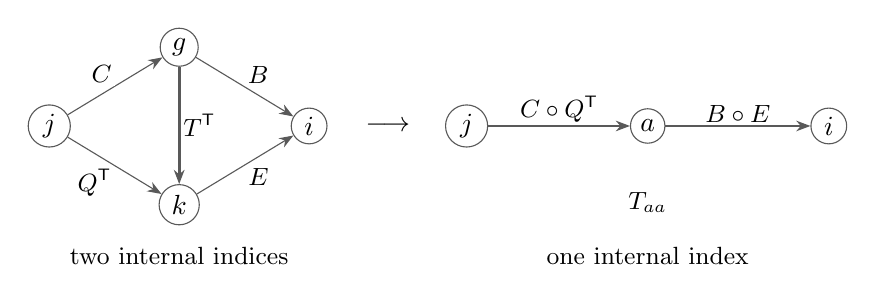
\begin{tikzpicture}[
  vertex/.style={circle,draw=black!65,fill=white,inner sep=2pt},
  edge/.style={-{Stealth[length=1.8mm]},draw=black!65},
  lab/.style={font=\small,fill=white,inner sep=1pt}]
 \node[vertex] (j) at (0,0) {$j$};
 \node[vertex] (g) at (1.65,1) {$g$};
 \node[vertex] (k) at (1.65,-1) {$k$};
 \node[vertex] (i) at (3.3,0) {$i$};
 \draw[edge] (j) -- node[lab,above left] {$C$} (g);
 \draw[edge] (j) -- node[lab,below left] {$Q^{\mathsf T}$} (k);
 \draw[edge] (g) -- node[lab,above right] {$B$} (i);
 \draw[edge] (k) -- node[lab,below right] {$E$} (i);
 \draw[edge,line width=1pt] (g) -- node[lab,right] {$T^{\mathsf T}$} (k);
 \node at (4.3,0) {$\longrightarrow$};
 \node[vertex] (jj) at (5.3,0) {$j$};
 \node[vertex] (v) at (7.6,0) {$a$};
 \node[vertex] (ii) at (9.9,0) {$i$};
 \draw[edge] (jj) -- node[lab,above] {$C\circ Q^{\mathsf T}$} (v);
 \draw[edge] (v) -- node[lab,above] {$B\circ E$} (ii);
 \node[font=\small,below=5mm of v] {$T_{aa}$};
 \node[font=\small] at (1.65,-1.65) {two internal indices};
 \node[font=\small] at (7.6,-1.65) {one internal index};
\end{tikzpicture}
\caption{Pinching the bridge in a crossed contraction.
The left network represents
$\sum_{g,k}B_{ig}E_{ik}T_{gk}C_{gj}Q_{jk}$.
Removing the off-diagonal entries of $T$ costs at most a fixed
operator-norm constant times $\max_{g\ne k}|T_{gk}|$.
Its diagonal identifies $g=k=a$, leaving
$(B\circ E)D_{\operatorname{diag}T}(C\circ Q^{\mathsf T})$.
The diagonal label is retained.}
\label{fig:network-pinching}
\end{figure}


\begin{proposition}[Opened conditional derivatives]
\label{prop:path-opened-derivative}
Fix a smooth multitime calculation as in
\Cref{lem:path-mixed-tensors}, a finite causal tree, common
Duhamel and likelihood truncations from
\Cref{lem:path-conditional-derivative}, and the tensor
approximations of \Cref{lem:path-increment-approximation}.
Require every linear-query edge of the calculation and every opened
$K$ edge to belong to the admitted path-matrix algebra, with its
entry predictions, and require all bounded coefficient labels to be
admitted path labels.  In particular, the calculation values are
admitted path recipes; the likelihood calculations above use $J$
and $J\circ J$ as their query matrices.  The broader class of
arbitrary bounded-operator query maps in
\Cref{lem:path-mixed-tensors} is not asserted to have this closure.
After ordinary conditional expectations are opened on their specified
causal branches, every remaining derivative contraction is a bounded
path matrix up to successive operator-norm errors.  It has vanishing
off-diagonal maximum and the Hadamard and diagonal predictions of
\Cref{lem:path-hadamard}.  The network errors have the typical,
weighted and integrated-parameter meaning of \Cref{def:path-tree}.
The earlier tensor and conditional truncation errors are uniform in
the joining state and stored parameters.
\end{proposition}

\begin{proof}
The first step removes errors that are uniform in the joining state.
Use \Cref{eq:path-copy-bound,eq:path-amplified-tail} for the tensor
approximations and the common $K$ tails.  At fixed accuracy, only
finitely many terms and fixed finite-measure Duhamel integrals remain.
Every $K$ insertion history is a bounded finite path-matrix word,
with a fixed cap on each likelihood label.  Keep ordinary $S$
expectations exact for now.  On opening a later inner-product or
replica test, they become ordinary causal branches and introduce no
new spatial summation index.

We now identify the two trees whose gluing represents an opened term.
The spatial recipe tree is the one constructed in
\Cref{lem:path-increment-approximation}.  A second, temporal tree
starts at the joining derivative coordinate: construct it by reading
the finite conditioning recursion backwards.  In
\Cref{eq:path-copy-tensors}, the memory term keeps its current
slot $p$.  The active term replaces $p$ by the newly introduced
slot $m$, through the $K$ path-word edge.  The mixed term forks
into $p$ and $m$, puts the $K$ edge on the latter branch, and
puts the bounded sign $-2x_p$ at the fork.  The new slot $m$ was
absent from the current derivative subset.  It therefore cannot
reconnect to an existing temporal leaf.  Repeating this construction
gives a temporal tree with one terminal for each original derivative
slot used in that term.  Finite causal-tree conditioning has the same
construction, with copies attached at the common joining vertex.

If a slot occurs several times in the recipe polynomial, append an
equality fork to its temporal terminal, one outgoing branch for each
occurrence.  Glue the resulting temporal leaves to the recipe leaves
in pairs, retaining the input-spin identity edges until this gluing
is complete.  Every leaf is paired.  The covering property ensures
that there is at least one leaf, and that both trees are connected.
Orient the temporal tree away from the joining derivative index and
the recipe tree toward its output site.  A directed path can cross
from the temporal tree into the recipe tree only at a paired leaf;
it cannot cross back.  Thus the glued network is acyclic, with its
unique source the joining derivative coordinate and its unique sink
the output site.  Every vertex is on a path between them.  The only
free indices are these two external ones; all internal indices are
ordinary equality contractions with no normalization factor.

The glued graph now has exactly the orientation required by
\Cref{lem:path-directed-network}.  Its matrix algebra, including
bounded visible dyads, is closed under ordinary products and
transposes.  Lemma~\ref{lem:path-hadamard} supplies the Hadamard
reduction and entry predictions for each newly formed fixed
expression.  Applying the network lemma therefore reduces the
opened term to the same path-matrix closure in operator norm.  The bounded scalar coefficients,
spin signs and diagonal predictions are path labels.  Integrate its
pointwise network bound over the fixed Duhamel parameter sets and
use the integrated entry predictions.  No worst auxiliary time or
starting configuration is selected.  The same argument applies to
stationary reversed causal branches.  Actual and predictor terms
keep the same subdivisions and approximations before they are
recombined and centered.

This proves closure for the opened histories used in the subsequent
conditional tests.  It does not assert a uniform-operator-norm
approximation of an arbitrary conditional matrix average by finitely
many sampled histories.  Conditional expectations remain exact
until those branches are opened.  For a still-averaged off-diagonal
maximum one may instead use conditional Jensen:
\[
 \max_{i\ne j}|\E[Q_{ij}\mid X]|
 \le\E[\max_{i\ne j}|Q_{ij}|\mid X].
\]
The uniform errors were removed before this typical network step.
In particular, no spatial square-mean error has been substituted for
an operator error.
\end{proof}

\subsection{Two-root self-averaging and completion of the calculus}

\begin{lemma}[Site histories from independent equilibrium roots]
\label{lem:path-two-root}
For two independent equilibrium samples in the same disorder, and
independent heat-bath site randomness on their trees, the limiting
joint site law of spin, field, and bounded likelihood histories is
the product of their one-root laws.  Consequently stationary site
means of any such bounded history label self-average in spatial
square mean.
\end{lemma}

\begin{proof}
We first separate the two planted starting directions, then propagate
that separation through the finite simulations.  Plant the samples
$\sigma$ and $\sigma'$.  Their overlap $r=n^{-1}\sigma^t\sigma'$
has the independent-uniform-spin law tilted by
$\exp(\beta^2nr^2/2)$, up to a spin-independent constant.  The
Rademacher rate function satisfies $I(r)\ge r^2/2$.
Since $\beta<1$, for every fixed $\varepsilon>0$ the probability
$|r|>\varepsilon$ is at most $e^{-c_\varepsilon n}$.
Conditionally on the spins the Gaussian disorder has the two rank
shifts
$\beta^2(\sigma\sigma^t+\sigma'\sigma'^t)/n$.
The two initial site spins are therefore asymptotically independent,
and the two planted directions are asymptotically orthogonal.

Perform the finite Gaussian recursion from
\Cref{lem:path-regression} for both causal simulations.  Each query
needed for spin and field histories is odd under global spin inversion
of its own root; a score query for likelihoods is also odd.  Fresh
refresh uniforms can be reflected under this inversion without changing
their law.  Deterministic cross-overlap limits of an odd query from
each different tree change sign under either inversion, and hence
vanish.  The Gaussian regression innovations for the two trees have
zero cross covariance and are independent.  By induction their
site recursions are independent, because their initial spins and site
seeds are independent as well.  Likelihood labels are bounded
functions of the resulting histories; their computation needs no
additional noncentered Gaussian query.  Thus their joint limits also
factor.  This induction does not apply to an arbitrary shared
noncentered query such as $J\1$, explaining the restriction in the
statement.

Transfer this factorization to the actual stationary paths using the
two-replica planting comparison and then
\Cref{prop:path-simulation,lem:path-likelihood-approximation}.  For
a bounded label $b$, represent the spatial mean of
$\E[b_i\mid J]^2$ by the empirical product on the two independent
roots.  The factorization makes its limit $(\tau b)^2$, proving
the claimed self-averaging of the site means.
\end{proof}

\begin{proof}[Completion of the proof of \Cref{thm:path-calculus}]
The required empirical space and endpoint predictions are supplied
by \Cref{lem:path-prediction}, together with orthogonality of hidden
vectors.  Lemma~\ref{lem:path-likelihood-approximation} puts the
likelihood labels in this construction with their stated tracial
convention.  The norm comparison then follows from
\Cref{lem:path-fock-norm,lem:path-sparse,lem:path-compressed}: the
representation is on one tree, retains the rare diagonal base, and
uses the Gaussian rate before paying the entropy and density costs.
The entry and Hadamard assertions come from
\Cref{lem:path-hadamard}; the difference and column-flip closure is
\Cref{lem:path-difference-closure}, with the opened conditional terms
just reduced to that closure.  Finally,
\Cref{lem:path-two-root} proves the restricted two-root independence
assertion.

Every construction used the fixed countable dense recipe family and
successive fixed approximations.  Diagonal extraction therefore gives
common high-probability disorder events for any finite initial list
of tests.  Lemma~\ref{lem:path-tree-transfer} permits polynomial
weights and actual conditional copies.  All superpolynomial path
discards were made separately on the original forward marginals.
These observations give the typicality convention and the order of
limits in the theorem.
\end{proof}

\section{A projected row likelihood and the spin spectral measure}
\label{sec:row-spin}

Projection onto the terminal configuration improves the moment bounds
for a row likelihood from exponential to subexponential in the path
length.  We prove this improvement first, keeping separate the roles of
the two estimates: unprojected moments justify passage to a fixed-time
limit, and projected moments determine the hidden-sector decay rate.
We then construct the spin spectral measure and derive the two strict
renewal inequalities needed to sum the hidden path expansion.

The inputs are the rough gradient and likelihood estimates of
\Cref{prop:path-rough}, the cavity density estimate of
\Cref{prop:stat-density}, and the following specified parts of
\Cref{thm:path-calculus}: deterministic stationary spin and path limits,
conditional prediction on causal trees, the noncrossing trace rule, and
the two-independent-equilibrium-sample comparison for spin histories,
fields, and likelihood labels.  The last comparison does not assert
independence of arbitrary recipes with noncentered queries or shared
random seeds.  The bridge argument below concerns an independent
\emph{removed Gaussian row}; it is not an application of a path rule to a
new bridge conditioned on two prescribed endpoints.

\subsection{The statement and its quantifiers}

Fix a row $i$ and $d>0$.  A mask $M\subset[0,d]$ is a deterministic
finite union of intervals specifying when the row perturbation is
present.  In the diagonal likelihood representation of
\Cref{prop:path-gradient}, let $\ell_i^M$ change the field at every site
$j\ne i$ by $-2X_i(s)J_{ij}$ when $s\in M$, leaving the site-$i$ update
rule unchanged.  The law with this modification has path density
$\ell_i^M$ with respect to the ordinary path law.  Put
\begin{equation}
 A_{i,x}^M(y)=\E_x[\ell_i^M\mid X_d=y].
 \label{eq:row-projection}
\end{equation}
This conditional expectation is the ratio of the modified and ordinary
terminal transition probabilities.  It includes paths on which the last
site-$i$ refresh left the spin unchanged, so the attempt and flip
likelihood conventions agree in \Cref{eq:row-projection}.

\begin{theorem}[Projected moments of a deterministic row likelihood]
\label{thm:row-projected-moments}
For each fixed real $r$ and each $\varepsilon>0$, there is
$d_0=d_0(r,\varepsilon)$ such that, for every fixed $d\ge d_0$ and every
deterministic mask $M$, outside a disorder event of probability tending
to zero there is a set $B_{n,d,M}$ satisfying
\begin{equation}
\mu(B_{n,d,M})\le e^{-c n},\qquad
 \max_i\E_x\bigl[(A_{i,x}^M(X_d))^r\bigr]
       \le e^{\varepsilon d}+o_n(1)
 \quad(x\notin B_{n,d,M}).
 \label{eq:row-moment-quantified}
\end{equation}
Here $c>0$ can depend on the fixed $d,r,\varepsilon$, but the estimates
in the proof are uniform in the deterministic mask.  Thus the notation
$e^{o_r(d)}$ for these moments always means dimension first and then
$d\to\infty$.  For $0\le r\le1$ the upper bound $1$ follows directly
from Jensen's inequality.  Negative $r$ in
\Cref{eq:row-moment-quantified} refers to the unrestricted positive
likelihood, not to a likelihood multiplied by a cutoff indicator.

The theorem also holds in its integrated form: if $M=M_\alpha$ ranges
over a deterministic measurable family with a finite measure on its
parameter space, the good disorder event can be chosen so that the
\emph{integrated} Gibbs mass of the exceptional starts is exponentially
small.  This includes masks determined by simplex times in a fixed
finite path expansion and the independent Poisson schedules used below.
It does not assert a simultaneous bound for a mask selected to maximize
an error after seeing the disorder.
\end{theorem}

The maximum over $i$ is obtained by a union bound over the $n$ rows,
applied after the exponential estimate for a row and a start.  This
exponential margin also allows any fixed polynomial weight and any
initial density bounded above by $e^{o(n)}$ in the integrated assertion.
We will use precisely these quantifiers in \Cref{thm:hidden-propagation}.

\subsection{The cavity identity and the last refresh}

We begin by expressing the projected likelihood through a cavity chain.
Remove row and column $i$, and let $Y$ be the resulting chain started
from $x_{-i}$.  Conditional on the cavity disorder, the removed vector
$(J_{ij})_{j\ne i}$ is independent Gaussian with covariance
$\beta^2 I/n$.  Let $N_j$ count the rate-one refresh attempts at $j$ and
let
\[
 M_j(t)=\sum_{s\le t:\,\text{refresh at }j}
       \bigl(Y_j(s)-m_j^Y(s-)\bigr),\qquad
 m_j^Y=\tanh((J^{(i)}Y)_j).
\]
These martingales are orthogonal, with predictable quadratic variations
$\int_0^t v_j^Y(s)\dd s$.  In the likelihood expansion we also retain
the clock-conditioned compensator $\int_0^t v_j^Y(s-)\dd N_j(s)$.

Let $\mathcal S$ be the site-$i$ refresh schedule. First condition on
a deterministic realization $\mathfrak s=(t_1,\ldots,t_m)$, with
$0<t_1<\cdots<t_m<d$.  The added spin $a$ stays constant between
successive scheduled times.  At a refresh its new value is sampled with
probability
\[
 p_\sigma(H)=\frac{e^{\sigma H}}{2\cosh H},
 \qquad H=\sum_{j\ne i}J_{ij}Y_j,
 \qquad\sigma\in\{-1,1\}.
\]
Set $\theta=1-2\1_M$.  Relative to the cavity experiment with these
site-$i$ coins, adding the field $\theta(s)a(s)J_{ij}$ at the other sites
has likelihood $L_\theta$.  Taylor expansion of $\log\cosh$ gives
\begin{align}
 \log L_\theta
 &=\sum_{h=0}^{m}\left(a_h Z_h-\tfrac12 B_h\right)+o_{\P}(1),
 \label{eq:row-score-expansion}\\
 Z_h&=\sum_{j\ne i}J_{ij}
                \int_{I_h}\theta(s)\dd M_j(s),\qquad
 B_h=\sum_{j\ne i}J_{ij}^2
                \int_{I_h}v_j^Y(s-)\dd N_j(s),
 \nonumber
\end{align}
where $I_h$ are the intervals between scheduled refreshes.  All changes
of the mask within $I_h$ remain inside a single stochastic integral.
Allowing arbitrarily many such changes therefore does not enlarge the
Gaussian list.  The absolute Taylor remainder is at most
\[
 C\max_{j\ne i}|J_{ij}|
       \sum_{j\ne i}J_{ij}^2N_j(d).
\]
At fixed $d$, this bound tends to zero in probability and admits the
moment truncations used below.  The time remains fixed before the
dimension limit throughout this expansion; it is never chosen as a
function of the dimension.

To keep track of the terminal spin, force its last refresh to take the
value $\sigma$, leaving the probabilities of all earlier coins
unchanged.  With $s_*=t_m$, define
\[
 \bar H_* =J_i\E_{x_{-i}}Y(s_*),\qquad
 q_\sigma=p_\sigma(\bar H_*),\qquad
 F_\sigma=\frac{p_\sigma(H(s_*))}{p_\sigma(\bar H_*)}.
\]
The elementary inequality $|\partial_H\log p_\sigma(H)|\le2$ gives
\begin{equation}
 e^{-2|H(s_*)-\bar H_*|}\le F_\sigma
                  \le e^{2|H(s_*)-\bar H_*|}.
 \label{eq:row-forced-coin}
\end{equation}
This ratio belongs inside the cavity average: it restores the random
last-spin probability after the deterministic reference probability has
been factored out.  Set $Z=Y(d)$ and define
\[
 A_{\theta,\sigma}(Z)
   =\E_{\mathrm{cav}}[L_\theta F_\sigma\mid Z],
\]
where the expectation includes the earlier site-$i$ coins and the
forced last coin.  When no refresh occurs, only one final spin is admissible, and
we set $q=1$ and $F=1$.  If $Q_d$ is the cavity terminal law, this
construction gives the exact kernel identities, conditional on
$\mathcal S=\mathfrak s$,
\begin{equation}
 \begin{aligned}
 P_\theta(X_i(d)=\sigma,Y(d)\in\dd z)
       =q_\sigma A_{\theta,\sigma}(z)Q_d(\dd z),
 \\
 A_{i,x}^{M,\mathfrak s}(\sigma,z)
       =\frac{A_{\theta,\sigma}(z)}{A_{1,\sigma}(z)}.
 \end{aligned}
 \label{eq:row-cavity-ratio}
\end{equation}
Here $A_{i,x}^{M,\mathfrak s}(y)=
\E_x[\ell_i^M\mid X_d=y,\mathcal S=\mathfrak s]$; the schedule
is still observed. The $r$th moment under the ordinary terminal law
conditional on that schedule is therefore
\begin{equation}
 \sum_\sigma q_\sigma
  \E_{Q_d}\!\left[A_{\theta,\sigma}^{\,r}
                         A_{1,\sigma}^{\,1-r}\right].
 \label{eq:row-ratio-moment}
\end{equation}
We have reduced the desired bound to fixed positive and negative
moments of two conditional cavity averages.  Their weights $q_\sigma$
sum to one even when the deterministic mean field $\bar H_*$ is large.

\begin{lemma}[Fixed-time moment passage]
\label{lem:row-uniform-integrability}
Fix $d$, a schedule, a mask, and $q<\infty$.  On the disorder events of
\Cref{prop:path-rough}, the positive and negative moments of $L_\theta$
are bounded by $e^{C_qd}$, uniformly in the schedule and mask.  The
variables $L_\theta F_\sigma$ have finite moments of every fixed positive
and negative order, with constants uniform in dimension at this fixed
$d$.  The same is true of their conditional averages given $Z$.
Bounded replicated-bridge tests, followed by these bounds, determine
both the positive and negative moments of the conditional averages in
the dimension limit.
\end{lemma}

\begin{proof}
Consider first a refresh at another site.  The logarithmic perturbation
is a Bernoulli likelihood increment with field displacement
$\theta aJ_{ij}$.  Its conditional exponential moment, at any fixed
real order, is at most
$\exp(C_qJ_{ij}^2)$.  Iteration over the attempts, followed by the Poisson
exponential formula, gives $e^{C_qd}$ because
$\sum_jJ_{ij}^2\le C$ and $\max_j|J_{ij}|=o(1)$.  The same calculation controls inverse moments.  After its prescribed
refresh the forced spin is predictable, so it does not change the
calculation.

We next control the forced-coin factor.  For $f(y)=J_iy$,
\Cref{prop:path-rough} supplies a fixed-horizon bound
on $\sup_y\norm{dS_sf(y)}^2$.  Applying
\Cref{lem:input-mgf} controls every fixed exponential moment of
$f(Y(s_*))-\E f(Y(s_*))$.  Combine this with
\Cref{eq:row-forced-coin} and H\"older's inequality.  The resulting constant may grow rapidly with fixed $d$.  This step
provides uniform integrability at fixed time, rather than a large-$d$
rate.

For a positive $V$ and $A=\E[V\mid Z]$, Jensen gives
\begin{equation}
 A^q\le\E[V^q\mid Z]\quad(q\ge1),\qquad
 A^{-q}\le\E[V^{-q}\mid Z]\quad(q>0).
 \label{eq:row-jensen-ui}
\end{equation}
Choosing an order strictly above the desired one gives uniform
integrability for the required powers of $A$.  To identify those powers
by replicated tests, take copies $V^{(1)},\ldots,V^{(b)}$ that are
conditionally independent given $Z$.  They satisfy
\[
 \E\left|b^{-1}\sum_{a=1}^bV^{(a)}-A\right|^2
       \le b^{-1}\E[V^2].
\]
Cap the $V^{(a)}$ first and pass to the dimension limit with the cap
and $b$ fixed.  Then let $b\to\infty$ and remove the cap.  The higher
moments in \Cref{eq:row-jensen-ui} justify this passage for positive and
negative powers alike; in particular, a limiting $A$ has no mass at
zero.  H\"older's inequality in \Cref{eq:row-ratio-moment} transfers the
conclusion to the terminal density ratio.
\end{proof}

\subsection{Replicated Gaussian bridges}

The terminal projection couples cavity paths through a common endpoint.
We represent that coupling by a shared Gaussian part, then show that
scores accumulated before a terminal buffer have a small shared part.
Their remaining private part can then be integrated in chronological
order. To construct the representation, fix the time $d$, the schedule, the moment
orders, and all preliminary truncations before taking the dimension
limit; $d$ will grow only later.  For each terminal state $Z$, take a
fixed number of conditionally independent cavity bridges from the same
specified start to $Z$.  On each branch, form the vector list
\begin{equation}
 \begin{aligned}
 \frac{Y(s)-\E Y(s)}{\sqrt n}\quad
       &\text{at the scheduled coin and last-field times},\\
 \frac1{\sqrt n}\int_{I_h}\theta\dd M
       \quad&\text{on the required score intervals}.
 \end{aligned}
 \label{eq:row-bridge-list}
\end{equation}
Conditional on these cavity data, projection by the independent removed
row gives an exactly Gaussian list, with covariance $\beta^2$ times
its Gram matrix.  The mean fields require a separate step: replace
$J_i\E Y(s)$ in the coin probabilities by formal deterministic
parameters $\bar h_s$.  We establish the averaged-test comparisons and
bounds uniformly in those parameters, and only then substitute the
actual values $\bar h_s=J_i\E Y(s)$.  This order avoids conditioning
the row on its own mean-field projections while continuing to use its
original Gaussian covariance.

To obtain the quenched statement, we now concentrate the averaged tests
in the removed row.  The required gradient bounds come from covariance
operators under the ordinary cavity path law.  For each unscaled
centered field vector in \Cref{eq:row-bridge-list}, that operator is
bounded by a constant depending only on $d$: apply the variance
conclusion of
\Cref{lem:input-mgf} to every deterministic linear combination of spins,
using \Cref{prop:path-rough}.  For an unscaled score vector the covariance
operator is bounded by $d$, directly by orthogonal martingale isometry.
Although the branches share an endpoint, each has the ordinary path law
as its unconditional marginal.  For a bounded smooth function $G$ of a
fixed list of row projections, Cauchy--Schwarz with the covariance
bounds therefore controls the Euclidean gradient of
$\E_{\mathrm{cav}}G$ by a constant depending only on the fixed list.
Since the row covariance is $\beta^2 I/n$, Gaussian concentration gives
error probability $e^{-c n}$ at each fixed accuracy.

We apply the same procedure to the brackets, first capping each site's
count.  With the cap fixed, concentration of a quadratic Gaussian form
gives
\begin{equation}
 B_h-\frac{\beta^2}{n}\sum_{j\ne i}
                   \int_{I_h}v_j^Y\dd N_j\longrightarrow0.
 \label{eq:row-bracket-replacement}
\end{equation}
Poisson tails remove the count cap from the averaged test, and the
moment bounds of \Cref{lem:row-uniform-integrability} then permit the
required moment passage.  The Taylor remainder in
\Cref{eq:row-score-expansion} is handled in the same order.  The site-$i$ coins are finite smooth
functions of the listed fields; after capping the tested likelihoods,
the same concentration estimate applies to their averages.  For uniformity in the deterministic mean fields, use a finite net on a
compact field range and then the limits of $p_\sigma(h+u)$ as
$h\to\pm\infty$, truncating the centered $u$ first.  This last step
allows the deterministic mean field to be unbounded.

It remains to transfer these estimates from a cavity start to a full
Gibbs start.  They are uniform over the start for every good cavity
matrix, and the two Gibbs laws satisfy
\[
 \frac{\mu_J(a,y)}{\mu_{J^{(i)}}(y)}
    =\frac{e^{aJ_iy}}{2\E_{\mu_{J^{(i)}}}\cosh(J_iY)}.
\]
Since $\norm{J_i}\le C$, the logarithm of this ratio has magnitude
$O(\sqrt n)$.  The change of measure therefore preserves each fixed exponential
failure rate.  A union bound over the rows followed by Markov's
inequality gives exponentially small quenched Gibbs mass of bad starts
on an event of disorder probability tending to one.  At this stage the
Gaussian description concerns bounded tests; its extension to moments
uses \Cref{lem:row-uniform-integrability}.

This Gaussian description does not require deterministic self-Grams.
The following representation retains their randomness while separating
the part shared by different bridges from the private Gaussian part of
each bridge. This is a specialized Dovbysh--Sudakov-type construction;
for the general representation, see Panchenko~\cite[Proposition~1,
equation~(1.2), and Lemmas~2--3]{Panchenko2010DS}. The finite-list
principal-coordinate proof needed here is given below, rather than
invoking the general representation theorem as a black box.

\begin{lemma}[Shared and private Gaussian parts]
\label{lem:row-hilbert-representation}
After subsequence extraction, a replicated array of the lists in
\Cref{eq:row-bridge-list} has the following representation.  Conditional
on a directing variable $\mathcal D$, each branch draws independently
its self-Gram matrix $Q$, its bracket data, and a list of vectors
$r_\alpha$ in one separable real Hilbert space.  Cross-Grams between
distinct branches are $\ip{r_\alpha}{r'_\gamma}$, and
$Q-(\ip{r_\alpha}{r_\gamma})_{\alpha,\gamma}$ is positive
semidefinite.  Include the factor $\beta$ in the vectors.  Conditional
on these data, the row projections have the form
\begin{equation}
 g(r_\alpha)+\xi_\alpha,
 \label{eq:row-shared-private}
\end{equation}
where $g$ is one common isonormal process and, independently on each
branch, $\xi$ is centered Gaussian with covariance
$Q-(\ip{r_\alpha}{r_\gamma})$.  Conditional averages in this
representation integrate one branch and its coins with $\mathcal D,g$
held fixed.
\end{lemma}

\begin{proof}
Begin with a finite-dimensional list and condition on $Z$.
Diagonalize
\[
 T=\E\left[\sum_\alpha u_\alpha\otimes u_\alpha\mid Z\right],
\]
where $u_\alpha$ denotes a normalized list vector.  Work first on the
sets where the list norms are bounded.  If $\Pi_k$ projects on the first
$k$ eigenvectors, independence of two branches and
$\Tr T\le K$ give
\[
 \E\left[\left|\ip{(I-\Pi_k)u_\alpha}
                           {(I-\Pi_k)u'_\gamma}\right|^2\Bigm|Z\right]
       \le\Tr[((I-\Pi_k)T)^2]\le\frac{K^2}{k+1}.
\]
Extract the laws of the finite coordinate lists together with their
self-Grams, and then let $k\to\infty$.  Count tails and the spin-norm
bounds remove the preliminary restriction on list norms.  The resulting
directing law on lists in $\ell^2$ identifies the limiting cross-Grams.
At every finite coordinate projection, the stated covariance difference
is positive semidefinite, and this property persists in the limit.  A common isonormal
process on $\ell^2$, plus independent Gaussians with the covariance
difference, realizes exactly these Gaussian Gram arrays.  The
conditional-average assertion follows from the replicated
approximation in \Cref{lem:row-uniform-integrability}.
\end{proof}

\subsection{The shared part of a prefix score}

The directing-law representation retains the information shared by
bridges with the same endpoint. We now show that scores accumulated
well before the terminal time have very little shared Gaussian part.  For this \emph{prefix score}
estimate, set $s=\sqrt d$ and $T=d-s$.  Split scores at $T$ when
necessary, leaving at most $m+2$ intervals.  The intervening suffix
allows us to use the cavity density bound.  Write $\kappa(s)$ for the
constant from the cavity version of \Cref{prop:stat-density}, so that
\[
 P_s^{\mathrm{cav}}(y,z)\le e^{n\kappa(s)}\mu_{\mathrm{cav}}(z),
 \qquad \kappa(s)\le C e^{-c s^{2/3}}.
\]
For any $a>0$, discard the endpoints at which
$Q_d(z)<e^{-an}\mu_{\mathrm{cav}}(z)$.  Their $Q_d$-probability is at
most $e^{-an}$.  On the retained endpoints, the joint law of two bridge
prefixes, after the common endpoint is integrated out, is dominated by
\begin{equation}
 e^{n(2\kappa(s)+a)}
       \times\text{the law of two independent cavity prefixes}.
 \label{eq:row-bridge-domination}
\end{equation}
Indeed its density given the two prefix endpoints $y,y'$ is
$\sum_zP_s(y,z)P_s(y',z)/Q_d(z)$, restricted to the retained $z$;
insert the preceding two bounds and sum $\mu_{\mathrm{cav}}(z)$.

We first estimate overlaps under the independent-prefix law, where the
normalized inner product of any two score vectors is centered.  Stop
each coordinate martingale when its clock count reaches a fixed large
polynomial in $d$.  The resulting product martingale has jumps bounded
by a polynomial in $d$ and bracket bounded by $n$ times a polynomial in
$d$.  The bounded-jump exponential martingale inequality then gives,
for any inverse-polynomial tolerance,
\begin{equation}
 \P\left(\left|n^{-1}\sum_j
        U_j^{(1)}U_j^{(2)}\right|>d^{-b}\right)
           \le 2e^{-n/d^{c_b}}.
 \label{eq:row-independent-overlap}
\end{equation}
Constants can absorb the fixed number of score positions.  Removing
the coordinate stopping changes normalized squared norms by an
arbitrarily small inverse power of $d$: the relevant bound is a
constant times $n^{-1}\sum_j N_j(d)^2\1_{N_j(d)>d^C}$, whose expectation
has this property and whose spatial average converges in probability.
These removals are made on each \emph{single bridge marginal}, which
is the ordinary path law, before using
\Cref{eq:row-bridge-domination}; a merely subexponential count-tail
bound is never multiplied by the bridge density.
Since $\kappa(\sqrt d)$ is smaller than every inverse power of $d$,
choose $a$ with the same property and apply
\Cref{eq:row-bridge-domination} to
\Cref{eq:row-independent-overlap}.  For all sufficiently large fixed
$d$, every prefix-score cross-Gram is bounded by an arbitrarily
prescribed inverse power of $d$ almost surely in the dimension limit.

The almost-sure bound on cross-Grams is the key output of this
comparison.  The next lemma converts it into a bound on shared-vector
norms; a small mean squared overlap would not suffice.

\begin{lemma}[An almost-sure overlap bound in a separable space]
\label{lem:row-overlap-norm}
If $r,r'$ are independent with the same law in a separable Hilbert
space and $|\ip r{r'}|\le\delta$ almost surely, then
$\norm r^2\le\delta$ almost surely.  The same assertion holds
conditionally on a directing variable.
\end{lemma}

\begin{proof}
Suppose a support point had squared norm greater than $\delta$.
Continuity would give a sufficiently small ball about it in which every
pair has inner product greater than $\delta$.  The ball has positive
probability, so independence makes this pair event have positive
probability, contradicting the hypothesis.  A countable base of balls
shows, by separability, that the law is carried by its support.  The
same argument applies to the conditional law for almost every directing
variable.
\end{proof}

Applying \Cref{lem:row-overlap-norm} position by position shows that the
shared vectors of prefix scores satisfy
\begin{equation}
 \max_{h:\,I_h\subset[0,T]}\norm{r_h}\le d^{-b}
 \quad\text{for every fixed }b,
 \label{eq:row-small-shared-score}
\end{equation}
once $d$ is large enough; the exponent in the preceding overlap test
is chosen twice as large.  The other shared vectors need not be small.
Their norms, and all self-Grams, have polynomial bounds in $d$.

We have controlled the shared prefix scores.  To use the private
scores chronologically, we also need the self-Gram identities supplied
by the single-path martingale calculation.  Distinct score intervals
are orthogonal; a score's squared norm equals its bracket in
\Cref{eq:row-bracket-replacement}; and each score is orthogonal to
every centered field observed at or before its interval begins.  For the last assertion, condition on that earlier
field and apply the martingale isometry to its scalar contraction
with the later score.  For score-score and score-square tests, use the
product martingale with the same count stopping as above.  In the
limit these are identities of the self-Gram data, not assertions that
those data have become deterministic.  Moreover
\begin{equation}
 \sum_{h:\,I_h\subset[0,T]} B_h\le \beta^2d,
 \qquad Q_{\mathrm{field},\mathrm{field}}\le4\beta^2.
 \label{eq:row-gram-budgets}
\end{equation}
The first inequality uses $v_j^Y\le1$ and the spatial law of large
numbers for the rate-one counts.  The second uses the deterministic
bound $\norm{Y(s)-\E Y(s)}^2\le4n$.

\subsection{The near-one Gaussian estimate}

The self-Gram identities prepare an adapted Gaussian calculation.
Subtracting the shared Gram leaves the private scores in
\Cref{eq:row-shared-private} with small covariances against earlier
scores and past fields, controlled by \Cref{eq:row-small-shared-score}.
We first correct those covariances to zero.  The correction is made
\emph{conditional on all the self-Gram and bracket data}, which may
still be random.

The correction must also work for a singular covariance matrix.  Set
the forbidden entries to zero, restore the score variances to $B_h$,
and add to the whole matrix a multiple of the identity equal to the
operator norm of that change.  The result is positive semidefinite.
For a fixed $K$, on schedules with at most $Kd$ refreshes, the list has $O_K(d)$
coordinates and its covariance has $O_K(d^2)$ entries. Its perturbation
norm is bounded by the number of coordinates times the largest changed
entry. Thus the added multiple $\delta_d$ can be smaller than any fixed
inverse power of $d$. The final score variances are
$b_h=B_h+\delta_d$, so $\sum_hb_h\le Cd$; replacing the original
compensators $B_h/2$ by $b_h/2$ costs only $O_K(d\delta_d)$.  Couple the original and corrected Gaussians through their
positive square roots.
The inequality
$\norm{Q^{1/2}-\widetilde Q^{1/2}}_{\op}
 \le C\norm{Q-\widetilde Q}_{\op}^{1/2}$
gives Gaussian errors with arbitrarily small polynomial variance.
The common score shifts $g(r_h)$ have the same property.

For each particular spin sequence the change in its coin weight is
bounded multiplicatively by
$\exp(2\sum_h|\Delta H_h|)$, and the change in its likelihood by
$\exp(\sum_h(|\Delta Z_h|+|\Delta B_h|/2))$.
The inequalities survive summation over spin sequences.  Since the
number of positions is $O(d)$, fixed exponential moments of the
comparison errors cost $e^{o(d)}$; increasing the inverse-polynomial
accuracy makes that cost $e^{o(1)}$.  Conditional H\"older inequalities
absorb these errors with an arbitrarily small additional change of
powers.  Thus the correction preserves the desired rate without a
lower bound on the eigenvalues of the covariance matrix.

\begin{lemma}[Chronological Gaussian integration]
\label{lem:row-adapted-gaussian}
Fix self-Gram and bracket data satisfying the corrected identities.
Treat all deterministic mean fields and all common field shifts as
arbitrary forcing.  Let $\widetilde Z_h$ be the corrected prefix
scores, of variances $b_h$, with $\sum_h b_h\le Cd$.
Let $a_h\in\{-1,1\}$ be the spin chosen using the fields and coins
available before score $h$, including a prescribed forced coin when
present.  For
\[
 W=\exp\left\{\sum_h a_h\widetilde Z_h
                         -\tfrac12\sum_h b_h\right\},
\]
one has, for every real $r$,
\begin{equation}
 \begin{aligned}
 \exp\left(-\tfrac12|r(r-1)|Cd\right)
 &\le\E[W^r\mid\text{self-Gram data and forcing}]\\
 &\le\exp\left(\tfrac12|r(r-1)|Cd\right).
 \end{aligned}
 \label{eq:row-near-one}
\end{equation}
In particular, powers within $\eta$ of one cost $e^{O(\eta d)}$.
\end{lemma}

\begin{proof}
Fix the specified data.  The full list is then Gaussian, and the
orthogonality identities make each score independent of the earlier
scores and of every field already used to choose its sign.  Its
variance is $b_h$.  It may remain correlated with fields at later coin
times, which does not affect this chronological calculation.  Generate
the Gaussian list and the coins in time order: the sign $a_h$ is
measurable before revealing $\widetilde Z_h$, so
\[
 \E\left[\exp\{r a_h\widetilde Z_h-r^2b_h/2\}
                      \mid\text{past}\right]=1.
\]
Their product has mean one.  Using $a_h^2=1$ and multiplying by
$\exp\{(r^2-r)\sum_hb_h/2\}$ proves the bounds.  Conditioning on
future self-Gram data is legitimate here because the needed Gaussian
orthogonality identities hold pointwise for each value of those data.
At no point are the scores themselves conditioned on future observed
fields.
\end{proof}

\subsection{Completion of the projected moment estimate}

\begin{proof}[Proof of \Cref{thm:row-projected-moments}]
The prefix is now controlled at powers close to one. Conditional
H\"older inequalities will put every fixed larger power on the short
suffix and on the last-spin factor. First retain schedules with at most
$Kd$ refreshes.  In the limiting representation, factor
\[
 L_\theta F_\sigma=W_{\mathrm{pre}}U,
 \qquad A=\E[W_{\mathrm{pre}}U\mid\mathcal D,g],
\]
where the prefix ends at $T=d-\sqrt d$ and $U$ contains the suffix and
the normalized last-spin factor, wherever that last refresh occurs.
For each fixed $q$, positive and negative moments of the suffix
likelihood are at most $e^{C_q\sqrt d}$.  Apply the forward martingale
calculation on the interval of length $\sqrt d$, and then use the
fixed-$d$ moment passage proved above.  The last-field factor has
bounded moments independent of $d$ in this limiting calculation:
its centered Gaussian field has variance at most $4\beta^2$ by
\Cref{eq:row-gram-budgets}, before the common and private parts are
separated.  H\"older therefore gives
\begin{equation}
 \E[|U|^q+|U|^{-q}]\le 2e^{C_q(1+\sqrt d)}.
 \label{eq:row-suffix-cost}
\end{equation}
The deterministic field means disappear from this bound through
\Cref{eq:row-forced-coin}.

For $0<\eta<1$, conditional H\"older gives the two inequalities
\begin{align}
 A&\le
  \E[W_{\mathrm{pre}}^{1+\eta}\mid\mathcal D,g]^{1/(1+\eta)}
  \E[U^{(1+\eta)/\eta}\mid\mathcal D,g]^{\eta/(1+\eta)},
 \label{eq:row-holder-upper}\\
 \E[W_{\mathrm{pre}}^{1-\eta}\mid\mathcal D,g]
 &\le A^{1-\eta}
       \E[U^{-(1-\eta)/\eta}\mid\mathcal D,g]^\eta.
 \label{eq:row-holder-lower}
\end{align}
For example, the second follows by writing
$W_{\mathrm{pre}}^{1-\eta}
 =(W_{\mathrm{pre}}U)^{1-\eta}U^{-(1-\eta)}$.
This second inequality supplies the inverse-moment bound: inverse
powers of $A$ are controlled by inverse powers of the prefix
conditional average together with positive powers of a suffix moment.

By \Cref{lem:row-adapted-gaussian}, each corrected prefix conditional
average with power $1\pm\eta$ lies between $e^{-C\eta d}$ and
$e^{C\eta d}$, uniformly in the branch data and common field forcing.
Jensen permits integration over the directing law and also taking
inverse powers.  The small common score and covariance-coupling
errors discussed above are handled by H\"older, with a power change
smaller than $\eta$.  Combining
\Cref{eq:row-holder-upper,eq:row-holder-lower,eq:row-suffix-cost} yields
for every fixed $p>0$
\begin{equation}
 \log\E[A^p+A^{-p}]
       \le C_p\eta d+C_{p,\eta}(1+\sqrt d)+o(d).
 \label{eq:row-final-rate}
\end{equation}
This inequality concerns the moments after the dimension limit.  Now
send $d\to\infty$ and then $\eta\downarrow0$.  The rough full-horizon
constants from \Cref{lem:row-uniform-integrability} served only to
identify these limiting moments; they contribute no additional term to
\Cref{eq:row-final-rate}.

H\"older's inequality in \Cref{eq:row-ratio-moment} proves the required
bound for every retained schedule. We next remove the schedule
conditioning. Under the ordinary path law, the tower property gives
\[
 A_{i,x}^M(X_d)
 =\E_x[A_{i,x}^{M,\mathcal S}(X_d)\mid X_d].
\]
The conditional expectation averages the schedule with its ordinary
conditional law given $X_d$. For $r\ge1$ or $r<0$, conditional Jensen
therefore decreases the moment when the schedule is no longer observed.  Control
the omitted schedules by a higher raw likelihood moment, H\"older's
inequality, and the Poisson estimate
\[
 \P\{N_i(d)>Kd\}\le e^{-d(K\log K-K+1)}.
\]
The raw bounds are uniform conditional on the schedule.  Taking $K$
large after the desired moment order makes this contribution smaller
than any prescribed $e^{-Hd}$.  The powers $0\le r\le1$ again follow
from Jensen.  This completes the moment estimate.

It remains to obtain the stated exceptional sets, including for an
integrated family of masks.  Fix $d$, the schedule-count cutoff, the
moment orders, and the comparison accuracies.  Every row concentration
constant above is then uniform in the mask parameters and deterministic
schedule times.  If
$\mathcal B(J,x,\alpha)$ denotes a failure of one of the finitely many
bounded tests, its row-and-start bound has the form
\[
 \E_J\int\mu_J(\dd x)\int
          \1_{\mathcal B(J,x,\alpha)}\,\nu(\dd\alpha)
       \le C e^{-cn}
\]
on the common good cavity events.  Apply Fubini at this point, before choosing the quenched event.  Markov's
inequality gives integrated Gibbs bad mass at most $e^{-cn/2}$ outside
an event of probability $Ce^{-cn/2}$.  If necessary, apply Markov once
more to remove starts with excessive bad-schedule mass, and use higher
rough moments to bound its contribution.  The countable approximations are fixed successively, with
arbitrary fixed slack, so their finite good events suffice before the
dimension limit.  Polynomial endpoint weights and an $e^{o(n)}$
initial density preserve negligibility.  At fixed times the remaining
integrands are dominated by the rough moment bounds and the relevant
mean-square vector budgets.

In a path expansion the order is therefore: fix the global time, hop
cutoff, shapes, elementary caps, moment orders, and label bins; integrate
over their deterministic simplex parameters; take dimension to
infinity; then remove caps and approximation errors; finally increase
the global time and decrease rate slack.  Annulus and first-exceedance
restrictions multiply a positive masked label by factors in $[0,1]$.
Its positive moments are bounded by those of the unrestricted label;
no inverse moment of a restricted label is used.  A selected start or
endpoint vector changes the weights in this integrated assertion and
does not choose an exceptional mask.  Likewise, good interior times
can be chosen from a positive-measure set after an integrated
estimate; a prescribed worst time is not being asserted to be good.
\end{proof}

\begin{corollary}[Stationary endpoint predictors]
\label{cor:row-stationary-predictors}
Let $a_i$ be a nonnegative row label on a span of length $d$, bounded
above by a masked likelihood $\ell_i^M$; factors $v_i\le1$ and cutoff
indicators are allowed.  Its stationary predictor at the right endpoint
has every fixed positive spatial moment bounded by $e^{o(d)}$.
The same bound holds after conditioning at a later endpoint.  Its
predictor at the left endpoint is bounded by one.  Raw fixed-order
moments cost at most $e^{C_pd}$.
\end{corollary}

\begin{proof}
For $p\ge1$, condition on both endpoints of the span and then apply
Jensen to the left endpoint's conditional law given the right endpoint.
The resulting integral over ordinary starts is bounded by
\Cref{thm:row-projected-moments}.  A higher raw moment and H\"older's
inequality make the exponentially small bad-start contribution
negligible.  The Markov property and stationarity make conditioning at
a later endpoint another $L^p$ contraction.  At the left endpoint,
the bound follows directly from
$\E_xa_i\le\E_x\ell_i^M=1$.  Powers between zero and one follow by
concavity.  The raw bound is \Cref{prop:path-rough}.
\end{proof}

\subsection{The positive spin spectral measure}

We turn to the spectral input for hidden propagation.  Let $E_n(\dd u)$
be the spectral resolution of $-L$ on $L^2(\mu)$, and encode the spin
coordinates by the positive matrix-valued measure
\[
 \mathsf M_n(\dd u)_{ij}
      =\ip{x_i}{E_n(\dd u)x_j}_\mu,
 \qquad \rho_n(\dd u)=\frac1n\Tr\mathsf M_n(\dd u).
\]
Spin inversion centers every $x_i$.  Consequently, $\rho_n$ is a
probability measure on the positive spectrum; on the good gap event,
its support lies in $[\gamma,\infty)$.  The heat-bath normalization
also identifies its first two moments:
\begin{equation}
 \begin{aligned}
 \int u\,\rho_n(\dd u)=\frac1n\sum_i\E_\mu v_i\le1,
 \\
 \int u^2\rho_n(\dd u)=\frac1n\sum_i\E_\mu(m_i-x_i)^2
                     =\frac1n\sum_i\E_\mu v_i.
 \end{aligned}
 \label{eq:spin-first-second}
\end{equation}
These bounds give tightness and uniform integrability of the first
moments.  The deterministic stationary spin limits from
\Cref{thm:path-calculus} identify a unique deterministic probability
measure $\rho$ to which the measures converge in probability.  Its
Laplace transform is
\begin{equation}
 C(t)=\int e^{-ut}\rho(\dd u)
     =\lim_{n\to\infty}\frac1n\sum_i\ip{x_i}{S_tx_i}_\mu.
 \label{eq:spin-correlation}
\end{equation}
Set
\[
 \lambda_{\rm sp}=\inf\supp\rho>0,
 \qquad R(t)=-C'(t)=\int u e^{-ut}\rho(\dd u).
\]
For \(z<\lambda_{\rm sp}\), put
\[
 \widehat R(z)=\int_0^\infty e^{zt}R(t)\dd t.
\]
The transform is finite and strictly increasing, and
$\widehat R(0)=1$.  All these definitions take dimension to infinity
first.

\begin{proposition}[Spin edge and the two renewal inequalities]
\label{prop:spin-spectrum}
For $0<\beta<1$,
\begin{equation}
 0<\lambda_{\rm sp}\le(1-\beta)^2,
 \qquad \beta\widehat R(z)<1,
 \qquad \beta^2\widehat R(z)<1-z
 \quad(z<\lambda_{\rm sp}).
 \label{eq:spin-conditions}
\end{equation}
Let $P_0(u)=1$, $P_1(u)=u$, and
$P_{k+1}(u)=uP_k(u)-P_{k-1}(u)$ be the monic second-kind Chebyshev
polynomials.  If
\[
 R_k(t)=\lim_{n\to\infty}\frac1n\Tr\left[
 P_k(J/\beta)\int u e^{-tu}\mathsf M_n(\dd u)\right],
\]
then
\begin{equation}
 \widehat R_k(z)=\beta^k\widehat R(z)^{k+1},
 \qquad z<\lambda_{\rm sp}.
 \label{eq:spin-trunk-transform}
\end{equation}
The limiting covariance trace density with respect to the semicircle
law $\rho_{\rm sc}$ on $[-2,2]$ is
\begin{equation}
 \lim_{n\to\infty}\frac1n
     \Tr\bigl[q(J/\beta)\E_\mu(xx^{\mathsf T})\bigr]
  =\int_{-2}^2\frac{q(u)}{1-\beta u+\beta^2}\rho_{\rm sc}(\dd u)
 \label{eq:spin-covariance-density}
\end{equation}
for every polynomial $q$.
\end{proposition}

\begin{proof}
The proof proceeds from a time-domain diagram identity to the transform
bound, then identifies the covariance trace density and tests its edge.
We first derive the diagram identity, making explicit the role of
stationarity.  Integration by parts and gradient intertwining yield
\begin{equation}
 R(t)=\lim_{n\to\infty}\frac1n\Tr\E_\mu[D_vK_tI].
 \label{eq:spin-gradient-trace}
\end{equation}
Here $K_tI$ applies $K_t$ to each constant coordinate vector.  Insert
the Duhamel expansion and use \Cref{thm:path-calculus}: visible
finite-rank terms vanish in normalized trace, each hop contributes
$\beta sD_v$, and the remaining trace is the sum of complete
noncrossing pairings.  Each resulting vertex carries the
product of its diagonal waiting likelihoods, its arrivals $v$, and
the bare factors $e^{-h}$.  These are nonnegative.  The root initially
carries $v$, as in \Cref{eq:spin-gradient-trace}.

The recurrence for $P_k(s)$ removes exactly the adjacent returning
contraction, making this polynomial the Wick string of $k$ consecutive
edges.  Each of its edges must therefore pair into the Duhamel walk.
Removing those $k$ pairs exposes an ordered trunk of $k+1$ completely
paired rooted time intervals.  Each interval starts with a $v$ weight,
including the interval at the original root, and each trunk edge
contributes $\beta$.  Conversely, concatenate $k+1$ rooted complete
diagrams and adjoin the outside Wick string.  This recovers one and only
one pairing, so no multiplicity factor appears.  After contraction, distinct vertices contribute scalar traces.
Stationarity makes each interval's trace depend only on its duration.
The separation into scalar factors comes from the noncrossing
contraction, rather than from temporal independence of intervals along
one spin history.  The spin/site self-averaging assertion in
\Cref{thm:path-calculus} is what identifies each such scalar factor
with its stationary trace when it is represented by independent
samples.  It is used only for spin, field, and likelihood labels.

The simplex integral over the successive interval lengths therefore
gives the convolution identity
\begin{equation}
 R_k(t)=\beta^k R^{*(k+1)}(t).
 \label{eq:spin-trunk-convolution}
\end{equation}
For the limiting argument, first keep time, Duhamel order, and likelihood
caps fixed.  Then \Cref{prop:path-rough} removes the caps and order
cutoff in the matrix $L^2$ comparison, establishing the identity at
each fixed $t$.  Because the complete-diagram terms are nonnegative,
we may also sum them monotonically when taking Laplace transforms.

To pass to transforms, we need a bound that is valid before the
dimension limit and does not require a finite-dimensional resolvent at
$z$.  Positivity supplies it: for a positive matrix $B$ and a
self-adjoint $Q$, $|\Tr(QB)|\le\norm Q_{\op}\Tr B$.
At finite $n$ apply this to the positive matrix
$\int u e^{-tu}\mathsf M_n(\dd u)$ and to
$Q=P_k(J/\beta)$.  The Wigner spectral bound and
$\sup_{[-2,2]}|P_k|=k+1$ show that, after the dimension limit,
\begin{equation}
 |R_k(t)|\le(k+1)R(t).
 \label{eq:spin-polynomial-domination}
\end{equation}
The same justification can be expressed through truncated integrals:
integrate the finite-dimensional inequality over $0\le t\le T$, take
the dimension limit, and then send $T\to\infty$.  The right-hand side
is integrable for $z<\lambda_{\rm sp}$.  Tonelli's theorem applied to
\Cref{eq:spin-trunk-convolution} now proves
\Cref{eq:spin-trunk-transform} and yields
\[
 (\beta\widehat R(z))^k\le k+1.
\]
Taking $k$th roots yields $\beta\widehat R(z)\le1$.  Given
$z<\lambda_{\rm sp}$, choose $z'$ strictly between them.  Since
$\widehat R$ is strictly increasing,
$\beta\widehat R(z)<\beta\widehat R(z')\le1$.

Integrating \Cref{eq:spin-trunk-convolution} at $z=0$ gives
\[
 \lim_{n\to\infty}\frac1n\Tr\left[
   P_k(J/\beta)\E_\mu(xx^{\mathsf T})\right]=\beta^k.
\]
Once again, justify the integral by first stopping at fixed $T$.
The spectral gap bounds the omitted covariance tail by
$\norm{P_k(J/\beta)}_{\op}e^{-\gamma T}$.  To identify the resulting
covariance density, use the orthonormality of the $P_k$ for
$\rho_{\rm sc}$ and the generating function
\[
 \sum_{k\ge0}\beta^kP_k(u)=\frac1{1-\beta u+\beta^2}
 \quad(-2\le u\le2);
\]
the series converges uniformly because $\beta<1$ and
$|P_k(u)|\le k+1$.  This proves
\Cref{eq:spin-covariance-density}.  The measure identified here is
positive: at finite $n$ it is the trace of the positive covariance
matrix against the spectral projections of $J/\beta$.

We next use this covariance density to bound the spin edge.  Fix a real
polynomial $q$.  Weighting $\mathsf M_n$ by $q(J/\beta)^2$ gives a
nonnegative scalar spectral measure, dominated by
$\norm{q(J/\beta)}_{\op}^2\rho_n$.  All its limiting mass therefore
lies in $[\lambda_{\rm sp},\infty)$, even though the finite-dimensional
spin measures may put small masses below that edge.  Its first moment
satisfies
\[
 \frac1n\Tr\bigl[q(J/\beta)^2D_{\E_\mu v}\bigr]
       \le\frac1n\Tr q(J/\beta)^2,
\]
because the energy matrix
$\int u\mathsf M_n(\dd u)$ is exactly $D_{\E_\mu v}$.
Use \Cref{eq:spin-covariance-density}, and then the semicircle trace
limit, to obtain
\begin{equation}
 \lambda_{\rm sp}
   \int\frac{q(u)^2}{1-\beta u+\beta^2}\rho_{\rm sc}(\dd u)
       \le\int q(u)^2\rho_{\rm sc}(\dd u).
 \label{eq:spin-edge-test}
\end{equation}
Alternatively, discard scalar spectral mass below
$\lambda_{\rm sp}-\delta$ before sending $\delta\downarrow0$.  This
gives the same inequality without requiring a uniform finite-$n$ lower
edge.
Choose $q_m(u)=((u+2)/4)^m$.  After normalization, the measures
$q_m^2\rho_{\rm sc}$ concentrate at $2$.  Letting $m\to\infty$ in
\Cref{eq:spin-edge-test} gives
$\lambda_{\rm sp}\le1-2\beta+\beta^2$.

Finally, for $0\le z<\lambda_{\rm sp}$,
\[
 \beta^2\widehat R(z)<\beta
       <2\beta-\beta^2
       \le1-\lambda_{\rm sp}<1-z.
\]
For $z<0$, $\widehat R(z)\le\widehat R(0)=1$ and
$\beta^2<1<1-z$.  These prove the second renewal inequality and
complete \Cref{eq:spin-conditions}.
\end{proof}

The two strict inequalities control different vertices in the path
expansion.  An ordinary interior trunk vertex has integrated weight
$\beta\widehat R(z)<1$.  If its initial variance factor is dropped,
we instead retain the bare waits and sum any number of paired side
excursions.  The resulting bound is the geometric renewal resolvent
\begin{equation}
 \frac1{1-z-\beta^2\widehat R(z)}<\infty.
 \label{eq:spin-exceptional-renewal}
\end{equation}
A bare wait contributes the transform $(1-z)^{-1}$.  Each inserted
excursion contributes two hops and one rooted paired interval, hence
the transform $\beta^2\widehat R(z)$.  Summing successive insertions
gives \Cref{eq:spin-exceptional-renewal}, with the bare waits retained
throughout.  The bound applies because $z<\lambda_{\rm sp}<1$.

\section{Averaging and propagation on the hidden complement}
\label{sec:hidden}

Assume $0<\beta<1$. Our objective is to bound propagation on the
complement of the recipe space. This bound separates the bulk spectral
edge from any slower eigenvalues visible in that space.
We use the typicality convention of \Cref{thm:path-calculus} for the
path law, endpoint vectors, and auxiliary trees throughout. Thus the
initial density is bounded above by $\exp(o(n))$ relative to equilibrium,
the pointwise bounds are polynomial in $n$, and dimension tends to
infinity before any approximation or large-time limit.
An endpoint vector $u$ is \emph{hidden} if
\[
 \E\abs{u^t B}^2\longrightarrow0
\]
for every fixed recipe vector $B$ at that endpoint. We write
$\norm{u}_2=(\E\norm{u}^2)^{1/2}$; the norm inside the expectation is
the unnormalized Euclidean norm. The same notation for a diagonal label
means $\norm{a}_{2,\tau}=\tau(a^2)^{1/2}$, and will always carry the
subscript $\tau$ to distinguish these two normalizations.

\begin{theorem}[Hidden propagation]\label{thm:hidden-propagation}
Let $\lambda_{\rm sp}$ be the spin spectral edge in
\Cref{prop:spin-spectrum}. For every $z<\lambda_{\rm sp}$ there is a
finite constant $C_z$ with the following property. Fix $t\geq1$, and let
$u=u(X_0)$ and $p=p(X_t)$ be polynomially bounded endpoint vectors with
bounded second moments. Suppose that $u$ is hidden, $p=df$ is an exact
gradient, and
\begin{equation}\label{eq:hidden-energy-hypothesis}
 \E\sum_j w_j(X_t)\norm{d_jp(X_t)}^2\leq C_t<\infty
\end{equation}
uniformly along the dimension sequence. Then
\begin{equation}\label{eq:hidden-propagation}
 \limsup_{n\to\infty}\abs{\E u^tK_t p}
 \leq C_z e^{-zt}
       \limsup_{n\to\infty}\bigl(\norm{u}_2\norm{p}_2\bigr).
\end{equation}
The constant does not depend on the bound in
\Cref{eq:hidden-energy-hypothesis}; that bound is allowed to depend on
the fixed time $t$. Equivalently, the rate on the right is
$\exp[-(\lambda_{\rm sp}-o(1))t]$, with the dimension limit taken first.
The assertion also holds in the integrated deterministic-time and mask
comparisons of \Cref{thm:path-calculus,thm:row-projected-moments}.
\end{theorem}

We first average a Wick string from its two endpoints, with at most
one vertex retaining its actual path label. We then control the endpoint
predictors by likelihood caps and sum the positive rooted excursions
at every parameter strictly below the spin edge. The derivative work
belongs to the averaging step: exactness converts
\Cref{eq:hidden-energy-hypothesis} into an unweighted Hessian bound
after a field cutoff.

\subsection{Wick strings and two-ended centering}
\label{subsec:hidden-wick}

Begin with fixed times, finitely many hops, and bounded diagonal labels.
In the word calculus, put $s=J/\beta$ and denote by
$B_k(a_0,\ldots,a_k)$ the Wick string with $k$ unpaired $s$-edges
and vertex labels $a_0,\ldots,a_k$. The normalization is
$B_0(a)=D_a$, and contracting adjacent edges around a vertex labeled
$a$ replaces that label by $\tau(a)$. Powers of $\beta$ are kept outside
this notation, so each actual path edge contributes a factor $\beta$.
Removing complete noncrossing excursions expresses a general path word
as a sum of Wick strings. At each surviving vertex, multiply the labels
from its repeated visits; keep the removed excursions as separate scalar
trace factors. The surviving labels have ordered time spans with
disjoint interiors.

In the Fock representation from \Cref{thm:path-calculus},
$s=l+l^*$ and $l^*D_al=\tau(a)I$. The Wick string is the sum of the
$k+1$ terms having creations to the left of a cut and annihilations to
its right. In particular,
\begin{equation}\label{eq:hidden-cut-bound}
 \norm{B_k(a_0,\ldots,a_k)}_{\op}
 \leq\sum_{h=0}^k \norm{a_h}_{\infty}
                     \prod_{j\ne h}\norm{a_j}_{2,\tau}.
\end{equation}
The norm here is taken in the representation with the full diagonal
base. A diagonal with support of limiting trace zero can still act on
that base. If it occurs at the cut, \Cref{eq:hidden-cut-bound} retains
its supremum norm.

There is also the exact splitting identity, for $0<r<k$,
\begin{align}
 B_k(a_0,\ldots,a_k)
 ={}&B_r(a_0,\ldots,a_{r-1},1)D_{a_r}
          B_{k-r}(1,a_{r+1},\ldots,a_k)\notag\\
 &-\tau(a_r)B_{r-1}(a_0,\ldots,a_{r-1})
          B_{k-r-1}(a_{r+1},\ldots,a_k).
 \label{eq:hidden-wick-split}
\end{align}
No subtraction is needed at an end vertex. For an interior vertex,
expand the Wick polynomial by inclusion--exclusion over disjoint
adjacent contracted pairs. The first line collects the choices that
leave the pair incident to $r$ uncontracted. The remaining choices
contract that pair and carry a minus sign, producing the second line.
This verification allows arbitrary vertex labels; constancy is not used.

For a label $a$ on a path from $0$ to $t$, let $a^0$ and $a^1$ denote
its stationary conditional predictors from $X_0$ and $X_t$,
respectively. They are the tracial predictors supplied by
\Cref{thm:path-calculus}, represented by bounded approximating recipes
in successive limits. Covariance identities require a different order:
choose a bounded path approximant and subtract its exact conditional
prediction. Keeping these operations distinct avoids a pointwise
regularity requirement on an exact quenched predictor at rare states.

\begin{lemma}[Two-ended averaging]\label{lem:hidden-averaging}
Let $a_0,\ldots,a_k$ be bounded path labels of the preceding kind.
Under the endpoint hypotheses of \Cref{thm:hidden-propagation},
\begin{align}
 B_k(a_0,\ldots,a_k)\ \sim\ 
 &\sum_{r=0}^k
 B_k(a^0_0,\ldots,a^0_{r-1},a_r,a^1_{r+1},\ldots,a^1_k)\notag\\
 &-\sum_{r=0}^{k-1}
 B_k(a^0_0,\ldots,a^0_r,a^1_{r+1},\ldots,a^1_k).
 \label{eq:hidden-averaging}
\end{align}
Here $T\sim T'$ means that $\E u(X_0)^t(T-T')p(X_t)$ tends to zero
after the prescribed successive approximations. The identity is an
identity in these bilinear tests, not an operator-norm replacement of
every path label by its predictor. The error will contain two
distinguished factors: one centered from the initial endpoint and one
from the terminal endpoint.
\end{lemma}

To prove the averaging identity, first isolate its algebraic error.
Multilinearity gives the exact difference between the two sides of
\Cref{eq:hidden-averaging}:
\begin{equation}\label{eq:hidden-double-centered-error}
 \sum_{0\le r<q\le k}
 B_k\bigl(a^0_{<r},\ a_r-a_r^0,\ a_{r<j<q},\
                    a_q-a_q^1,\ a^1_{>q}\bigr).
\end{equation}
Telescope at the first mismatch from the left and then telescope the
remaining suffix from the right. The all-initial term cancels the
last term of the second telescope. Thus
\Cref{eq:hidden-double-centered-error} retains the actual labels
between the two distinguished vertices. It remains to prove that each
doubly centered summand has zero limiting bilinear test.

The first use of the next lemma is to cut off large terminal fields
before estimating the Hessian. A localized endpoint vector can give
those fields substantial Euclidean mass even when their spatial trace
is small. The two centered factors make their removal possible in the
present bilinear test.

\begin{lemma}[Small-trace replacements in a centered string]
\label{lem:hidden-small-trace}
Consider a summand of \Cref{eq:hidden-double-centered-error}. Its
bounded labels may be approximated in tracial $L^2$ while keeping the
two distinguished factors centered at their respective endpoints.
The error in the hidden bilinear test tends to zero with the tracial
errors. A bounded diagonal of vanishing trace support can also be
inserted at the terminal endpoint at zero cost in this test.
\end{lemma}

\begin{proof}
The Fock comparisons in this proof first remove the terminal visible
component, as in the endpoint projection argument used below for the
predictor caps.  Fix a finite family of endpoint recipes with nonsingular
limiting Gram matrix, and let $Q_m$ be their actual orthogonal projection
on the corresponding Gram-good event, and zero off that event.
Both $Q_m$ and $I-Q_m$ are contractions.  For every fixed capped path word
$W$, Cauchy--Schwarz bounds the removed pairing by
$\|Q_mW^tu\|_2\|p\|_2$, which tends to zero at fixed $m$ by
Assertion~\textup{(ii)} of \Cref{thm:path-calculus} and the fixed inverse
Gram bound.  The weighted typicality convention removes the exceptional
Gram event.  Exhaust the endpoint recipe completion, omitting null
directions, and choose $m=m(n)\to\infty$ sufficiently slowly that these
errors vanish for every fixed word and $(I-Q_m)p$ is hidden for every
fixed endpoint recipe.  Its second-moment and polynomial bounds follow
from contraction.  The projection depends only on the shared endpoint
and its fixed seeds, so permutations of the replicated branches preserve
it.  This projection is used only for the Fock bilinear comparisons;
we retain the original exact $p$ for the Hessian estimates that follow.

Work on one finite tree and use the cut expansion behind
\Cref{eq:hidden-cut-bound}. Every cut away from the replaced factor
puts that factor on a pure creation or pure annihilation side. Its trace
two-norm then bounds the error, multiplied by the fixed bounds on the
other factors and the two endpoint norms. Only the cut at the replaced
factor needs another argument. At that cut, at least one distinguished
centered factor lies on the pure side leading to its own centering
endpoint.

Attach $b$ conditionally independent copies at this endpoint. Lift
this single replicated star to the Fock representation, and symmetrize
by taking a direct sum over permutations of the copies. Repeatedly
applying $l^*D_al=\tau(a)I$ expresses inner products of pure-side strings
as products of pair traces. For different copies, one factor is the
pair trace of the centered label and has zero limit. With approximated
predictors, bound its absolute value by $\eta$, tending to zero with
the approximation. Write $C_\alpha$ for the pure-side creation operator
on copy $\alpha$, oriented toward the shared endpoint. The Gram bounds
are
\[
 \norm{C_\alpha^*C_\alpha}\leq C,\qquad
 \norm{C_\alpha^*C_\gamma}\leq C\eta\quad(\alpha\ne\gamma),\qquad
 \norm{[C_1\ \cdots\ C_b]}^2\leq C(1+(b-1)\eta).
\]
If $v$ denotes the vector at the shared endpoint, symmetry of the
lifted star gives
\[
 \E\norm{C_1^*v}^2
 =\frac1b\sum_{\alpha=1}^b\E\norm{C_\alpha^*v}^2
 \leq C(b^{-1}+\eta)\E\norm{v}^2.
\]
The vector at the opposite end may depend on its whole branch;
Cauchy--Schwarz now bounds the squared bilinear contraction by
\[
 C\bigl(b^{-1}+\eta\bigr)\norm{u}_2^2\norm{p}_2^2.
\]
The fixed caps bound the diagonal Gram blocks. Apply Cauchy--Schwarz
and take the limits $n\to\infty$, $\eta\to0$, and $b\to\infty$ in
that order to obtain zero. All cuts for this replacement are treated
on the same star. The argument makes no simultaneous choice of
creation operators on stars rooted at different endpoints.

A terminal insertion with small trace support has the same two cases.
Every nonterminal cut pays its trace two-norm; at the terminal cut,
the left distinguished factor lies on its centered pure side, so the
replication argument applies. Iterate for finitely many replacements.
When the replaced factor is an approximated distinguished label,
keep its exact forward or backward subtraction throughout this step
and use the other distinguished factor at the exceptional cut.

The word comparison retains every rare diagonal's action on the base.
Small trace is used on a pure side, and centering treats the remaining
cut; neither step uses the false implication
$\tau(c^2)\to0\Rightarrow\norm{D_c}_{\op}\to0$.
\end{proof}

\subsection{The Hessian cutoff and the covariance norm}
\label{subsec:hidden-covariance}

The covariance proof will pair a terminal Hessian with a matrix in
Hilbert--Schmidt norm. We first obtain the required unweighted Hessian
bound. Let $h_i(x)=(Jx)_i$ and choose a smooth function $\chi_M$ equal to one
on $[-M,M]$, vanishing outside $[-M-1,M+1]$, and with uniformly bounded
first derivative. In each double-centered test, replace $p$ by
\[
 p^{(M)}_i(x)=\chi_M(h_i(x))p_i(x).
\]
As $M\to\infty$, the field tail has vanishing spatial trace.
\Cref{lem:hidden-small-trace} therefore justifies this replacement
inside each double-centered test. This use of $p^{(M)}$ does not
require unweighted-norm approximation of an arbitrary localized $p$.

Write $dp=(d_jp_i)_{i,j}$, with the component index as row and the
derivative index as column. The exact product rule is
\begin{equation}\label{eq:hidden-product-rule}
 d_j(fg)=f\,d_jg+g\,d_jf-2x_j(d_jf)(d_jg),
 \qquad f(x^j)=f(x)-2x_jd_jf(x).
\end{equation}
Using the second form of this rule gives
\[
 d_jp_i^{(M)}
 =\chi_M(h_i(x^j))d_jp_i+p_i\,d_j\chi_M(h_i).
\]
For sufficiently large $n$, $\max_{ij}|J_{ij}|\leq1$. On the support
of the first coefficient, $|h_i(x)|\leq M+3$, and hence
$w_i(x)\geq c_M>0$. Mixed-gradient symmetry and the row square bound
therefore give the pointwise estimate
\begin{align}
 \norm{dp^{(M)}}_{\HS}^2
 &\leq C_M\sum_{i,j}w_i|d_ip_j|^2
       +C\sum_i p_i^2\sum_jJ_{ij}^2\notag\\
 &\leq C_M\sum_i w_i\norm{d_ip}^2+C\norm{p}^2.
 \label{eq:hidden-cutoff-hessian}
\end{align}
The cutoff supplies the bounded unweighted mean-square Hessian
needed below. This conversion is the averaging proof's only use of
the symmetry $d_jp_i=d_ip_j$.

We will absorb fixed smooth endpoint words into the terminal vector,
so we also need preservation of this Hessian bound. Check the two
generators, a bounded diagonal $D_f$ and $J$. For a diagonal, write
$Df=(d_jf_i)_{i,j}$ and use
\begin{equation}\label{eq:hidden-matrix-product-rule}
 d(D_fq)=D_f\,dq+D_q\,Df-2(Df\circ dq)D_x.
\end{equation}
The derivative matrix $Df$ has bounded operator norm by the smooth
recipe calculus. Consequently
$\norm{D_qDf}_{\HS}\leq\norm{q}\norm{Df}_{\op}$, and the other two
terms are controlled by $\norm{dq}_{\HS}$. Multiplication by $J$ costs
its bounded operator norm. These estimates, with the exact last term
of \Cref{eq:hidden-matrix-product-rule}, prove the assertion by
induction through the endpoint word.

The second preparation concerns a correlated hidden vector. We need a
pointwise operator estimate for a conditionally averaged derivative,
because a tracial or averaged Hilbert--Schmidt error need not remain
small after its rows are weighted by that vector.

At a joining time $s$, condition on $X_s=x$ and the realized past $\pi$.
For a fixed smooth multitime site-vector calculation $F$ satisfying
\Cref{lem:path-mixed-tensors}, put
\[
 A(x,\pi)=d_x\E[F\mid X_s=x,\pi],
\]
with output as row and derivative index as column. First take the
conditional expectation. \Cref{lem:path-conditional-derivative}
then supplies common linear truncations $A_N$ with
\begin{equation}\label{eq:hidden-conditional-op}
 \norm{(A-A_N)^tc}(x,\pi)
 \leq C_F\varepsilon_N\norm c,\qquad
 \sup_{x,\pi}\norm{A-A_N}_{\op}\leq C_F\varepsilon_N,
 \quad\varepsilon_N\downarrow0.
\end{equation}
The first inequality holds for every output vector $c$ at the same
fixed $(x,\pi)$, using the same truncation. Taking its supremum over
$c$ therefore gives the operator estimate before any expectation.

Recall why this lemma applies to multitime labels. Their mixed tensors
retain at most one difference in each observed-state slot. When a
conditional starting state $z$ is copied into a stored parent $y$, the
exact rule is
\[
 d_j[G(y,z)|_{z=y}]
 =[d_j^yG+d_j^zG-2y_jd_j^yd_j^zG]_{z=y}.
\]
The mixed correction is among those retained tensors. The finite
leaf-elimination argument of \Cref{lem:path-conditional-derivative}
uses point-start $K$ bounds on the evolving index, with all other
indices as Hilbert coordinates; copying indices is a norm-one
coordinate restriction. It approximates the differentiated conditional
expectation itself, rather than differentiating an approximation to
its value. Thus, even when $u=u(X_0)$ is correlated with $(x,\pi)$,
\begin{equation}\label{eq:hidden-row-weighted-error}
 \norm{D_u(A-A_N)}_{\HS}^2
 =\sum_i|u_i|^2\norm{\operatorname{row}_i(A-A_N)}^2
 \leq C_F^2\varepsilon_N^2\norm{u}^2.
\end{equation}
This is the row-weighted truncation bound used in the covariance
calculation below.

Apply the operator estimate before opening auxiliary paths. Then
\Cref{lem:path-increment-approximation,prop:path-opened-derivative}
approximate the fixed mixed tensors by tensor networks in operator
norm and place their opened contractions in the path-matrix closure.
The retained matrices satisfy the entry and Hadamard rules of
\Cref{thm:path-calculus}. This concerns fixed capped histories after
opening; it gives no operator-norm approximation of an arbitrary
conditional expectation by finitely many Monte Carlo samples.

\begin{lemma}[A marked continuing derivative]\label{lem:hidden-marked-spine}
Fix an opened, capped derivative history of one smooth multitime
label. Suppose it has an entering derivative index, at least one
branch differentiating that label, and one derivative index continuing
to a later factor. Its temporal derivative tree has a unique path
between the entering and continuing indices. Absorb the part before
its first label attachment into the incoming propagation matrix, and
retain the part after its last attachment as a subsequent bounded
propagation. Let $M$ be the matrix arriving at the first attachment,
with label site as row and derivative index as column.

If $\Phi(M)$ is the matrix after the intervening history, then, in the
finite-tree comparison,
\begin{equation}\label{eq:hidden-marked-spine-bound}
 \norm{\Phi(M)}_{\HS}
 \leq C\norm{\diag(M)}+o(1)\norm{M}_{\HS}.
\end{equation}
Here $C$ depends on the fixed circuit and capped history. All memory
copies and all mixed differences of the label are included in this
history. The estimate does not replace a mixed label tensor by an
ordinary first Jacobian.
\end{lemma}

\begin{proof}
First fix a tensor-network approximation from
\Cref{lem:path-increment-approximation}. Before opening paths, use
the mixed-tensor budget to bound its operator errors, and remove
those errors in the prescribed successive approximation limit.
The temporal tree off the marked path consists of disjoint subtrees
ending at derivative leaves of the chosen label. Each attachment has
at least one such leaf. The corresponding maps are bounded tensor
products and compositions of capped path matrices and equality
copies; every equality copy has norm at most its fixed scalar label
bound. Pull their adjoints into the row tensor of the label circuit.
Repeated occurrences of a derivative index are handled by the
norm-one equality embedding. The resulting tensor $U_i$ on the $r$
attachment indices satisfies
\begin{equation}\label{eq:hidden-marked-row-tensor}
 \sup_i\sum_{a_1,\ldots,a_r}|U_i(a_1,\ldots,a_r)|^2\leq C^2.
\end{equation}
Use the operator norm of each flattened mixed tensor to bound each
of its rows in Euclidean norm. The off-path maps act on disjoint
groups of leaves, so their tensor-product operator norms give the
stated estimate without a dimension factor.

Suppress vertices on the marked path with no label attachment. The
matrices between its remaining consecutive attachments are bounded
path matrices $Q_1,\ldots,Q_{r-1}$. For $r\geq2$, put
\begin{equation}\label{eq:hidden-marked-kernel}
 L_i(a_1,a_r)=\sum_{a_2,\ldots,a_{r-1}}
 U_i(a_1,\ldots,a_r)\prod_{\ell=1}^{r-1}
                       (Q_\ell)_{a_\ell a_{\ell+1}}.
\end{equation}
Then $\Phi(M)_{i,b}=\sum_a M_{i,a}L_i(a,b)$. If $r=1$, this formula
means $L_i(a,b)=\1_{a=b}U_i(a)$.

The next step is to make every $Q_\ell$ in
\Cref{eq:hidden-marked-kernel} diagonal. Control one replacement at
a time: fix an edge $e$ and put $Q_e^{\rm off}$ there. With the
endpoints fixed, Cauchy--Schwarz bounds the squared kernel by
\[
 \left(\sum_{a_2,\ldots,a_{r-1}}|U_i(a_1,\ldots,a_r)|^2\right)
 \left(B_1\cdots B_e^{\rm off}\cdots B_{r-1}\right)_{a_1a_r},
\]
where $B_\ell=|Q_\ell|^{\circ2}$ entrywise. Every row sum and every
column sum of $B_\ell$ is at most $\norm{Q_\ell}_{\op}^2$.
Writing $\eta_e=\max_{a\ne b}|(Q_e)_{ab}|$, we have
$B_e^{\rm off}\leq\eta_e^2\1\1^t$ entrywise. The second factor is
therefore at most
\[
 \eta_e^2\prod_{\ell\ne e}\norm{Q_\ell}_{\op}^2.
\]
Sum over the endpoints and use \Cref{eq:hidden-marked-row-tensor}.
This gives
\[
 \sup_i\norm{L_i^{(e,\rm off)}}_{\HS}
 \leq C\eta_e\prod_{\ell\ne e}\norm{Q_\ell}_{\op}.
\]
The estimate remains valid after any other edges have been made
diagonal. Telescope over the finitely many edges and apply the entry
rule in \Cref{thm:path-calculus} to obtain
$\sup_i\norm{L_i-L_i^{\rm diag}}_{\op}=o(1)$. Its row action costs
at most $o(1)\norm{M}_{\HS}$.

After these replacements, diagonal marked-path edges force all
attachment indices to agree. The remaining action takes the form
$M\circ E$, where
\[
 E_{i,a}=U_i(a,\ldots,a)
                \prod_{\ell=1}^{r-1}(Q_\ell)_{aa}.
\]
This $E$ contains the entire label derivative subnetwork, including
its memory copies. It is the two-terminal network obtained by tying
all temporal attachment indices to the common source $a$, with the
label output $i$ as sink. Every derivative leaf is paired.
\Cref{lem:path-directed-network,prop:path-opened-derivative} place it
in the bounded path-matrix closure. The diagonal factors above may
first be replaced by their uniformly accurate diagonal predictions.
Consequently $\max_i|E_{ii}|\leq C$ and
$\max_{i\ne a}|E_{i,a}|=o(1)$. The estimate
\[
 \norm{M\circ E}_{\HS}^2
 \leq C^2\norm{\diag(M)}^2
       +\max_{i\ne a}|E_{i,a}|^2\norm{M}_{\HS}^2
\]
proves \Cref{eq:hidden-marked-spine-bound}. Here the entry estimates are used on fixed typical finite trees,
followed by their integrated comparison. Their scope does not include
uniformity over arbitrary states.
\end{proof}

\begin{figure}[htbp]
\centering
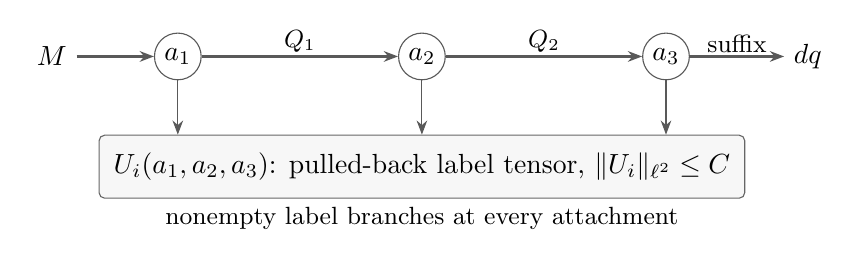
\begin{tikzpicture}[
  vertex/.style={circle,draw=black!65,fill=white,inner sep=2pt},
  edge/.style={-{Stealth[length=1.8mm]},draw=black!65},
  lab/.style={font=\small,fill=white,inner sep=1pt}]
 \node (in) at (0,0) {$M$};
 \node[vertex] (a) at (1.6,0) {$a_1$};
 \node[vertex] (b) at (4.7,0) {$a_2$};
 \node[vertex] (c) at (7.8,0) {$a_3$};
 \node (out) at (9.6,0) {$dq$};
 \draw[edge,line width=1pt] (in) -- (a);
 \draw[edge,line width=1pt] (a) -- node[lab,above] {$Q_1$} (b);
 \draw[edge,line width=1pt] (b) -- node[lab,above] {$Q_2$} (c);
 \draw[edge,line width=1pt] (c) -- node[lab,above] {suffix} (out);
 \node[draw=black!60,rounded corners=2pt,fill=black!3,
       minimum width=8.2cm,minimum height=8mm]
       (tensor) at (4.7,-1.4)
       {$U_i(a_1,a_2,a_3)$: pulled-back label tensor,
        $\|U_i\|_{\ell^2}\leq C$};
 \draw[edge] (a) -- (a |- tensor.north);
 \draw[edge] (b) -- (b |- tensor.north);
 \draw[edge] (c) -- (c |- tensor.north);
 \node[font=\small] at (4.7,-2.05)
      {nonempty label branches at every attachment};
\end{tikzpicture}
\caption{The derivative continuing into the later suffix defines
a marked path.  Side branches are absorbed into a label tensor
with bounded row square norm.  After branch-free segments have been
combined, every intervening $Q_r$ separates two nonempty sets of
label leaves.  Its off-diagonal contribution is small by
Cauchy--Schwarz and the row and column sums of the squared-entry
matrices.  Pinching all such segments ties the attachment indices
and returns the diagonal estimate for $M\circ E$.}
\label{fig:marked-continuation}
\end{figure}


\subsection{Proof of the averaging identity}
\label{subsec:hidden-averaging-proof}

\begin{proof}[Proof of \Cref{lem:hidden-averaging}]
Fix a summand of \Cref{eq:hidden-double-centered-error}, with
distinguished labels
$a=a_r-a_r^0$ and $b=a_q-a_q^1$, where $r<q$. By
\Cref{lem:hidden-small-trace}, approximate its path labels by fixed
bounded smooth multitime circuits, with every observed state inside
the label's time span. These circuits may contain mixed queries such
as $J[f(X_s)\odot X_r]$; no representation as a sum of separated
single-time products is required. The frozen-score construction of
\Cref{lem:path-likelihood-approximation} puts its smooth caps in the
class of \Cref{lem:path-mixed-tensors}; in particular, outside spins
multiplying an unbounded query are handled by its finite
sign-pattern decomposition. Before estimating derivatives, fix the circuit, its cap, and every
observation time. Keep both distinguished vertices exactly
conditionally centered for each approximant. Approximate the
nonspecial endpoint factors by fixed smooth one-state functions
before the derivative limits, and perform the field cutoff above.
Its threshold and the suffix approximants remain fixed throughout
the derivative comparisons.

For the exact right predictor, use a conditional path representation
instead of requiring a regular one-state recipe. Represent its value
by an independent ordinary stationary-kernel path from $X_t$, reading
the multitime evaluations in reverse order. Differentiate by propagating
the full mixed-slot recursion down this added causal branch.
Its tensor and path-network conclusions are those of
\Cref{lem:path-conditional-derivative,prop:path-opened-derivative}.
Keep the exact conditional subtraction before opening any of these
derivatives. The conditional estimates
\Cref{eq:hidden-conditional-op,eq:hidden-row-weighted-error} apply
there as well. The error in replacing a tracial predictor by this
exact prediction is handled before derivatives are opened, by
\Cref{lem:hidden-small-trace}.

Split the Wick string at $a$ and $b$ using
\Cref{eq:hidden-wick-split}. The subtractions involving $\tau(a)$ or
$\tau(b)$ vanish; errors from approximate trace centering are
controlled in the unsplit Wick form by
\Cref{lem:hidden-small-trace}. Absorb the outer strings into the
endpoint vectors. The left vector remains hidden by
\Cref{thm:path-calculus}; the right vector has bounded mean-square
unweighted Hessian by \Cref{eq:hidden-cutoff-hessian} and
\Cref{eq:hidden-matrix-product-rule}. It remains to prove
\begin{equation}\label{eq:hidden-covariance-target}
 \E u(X_0)^tD_a QD_b p(X_t)\longrightarrow0,
\end{equation}
where $Q$ is a positive-length Wick string with identity end labels.
The left centered label $a$ will give a martingale covariance. If its
paired derivative reaches $p$, the backward centering of $b$ will
cancel the term. If the derivative first hits a tail label, the
nonempty Wick prefix will supply the cancellation instead.

To prove the remaining bilinear limit, use conditional martingale
covariance up to the last evaluation in $a$. For scalar future
observables $F,G$, it reads
\begin{equation}\label{eq:hidden-martingale-covariance}
 \Cov_x(F,G)
 =2\E_x\int\sum_j w_j(X_s)
              d_jF_s(X_s)\,d_jG_s(X_s)\dd s,
\end{equation}
where $F_s,G_s$ are the conditional future expectations with their
already observed arguments held fixed. The integration stops once
$F$ is fully observed. To check the factor, a flip of $j$ has rate
$w_j/2$ and changes a scalar martingale by $-2x_jd_jF_s$; its product
bracket is $2w_jd_jF_s d_jG_s$. Since $a$ has exact forward conditional
mean zero, \Cref{eq:hidden-covariance-target} is the corresponding
covariance, with $u(X_0)$ fixed under the initial conditioning.

\Cref{eq:hidden-martingale-covariance} introduces a derivative
index in addition to the sites of the Wick string. Propagate the two
derivatives by the mixed-slot recursion and $dS_h=K_hd$, including
every exact product and memory-copy correction. First conditionally average the factor differentiating $a$ and
remove its truncation with \Cref{eq:hidden-row-weighted-error}.
On the other side, each terminal tensor term contains $p$ or $dp$
exactly once, because $p$ has only the terminal state slot. The bounded mixed label tensors and the Hilbert-space
amplification of \Cref{prop:path-rough} therefore propagate its
unweighted mean-square Hilbert--Schmidt budget. Tensor and
propagation errors are removed in these norms before paths are
opened. For the retained histories use
\Cref{prop:path-opened-derivative} to reduce their complete
derivative subnetworks to bounded path matrices. The two conditional
future expectations in
the covariance can then be represented by independent causal futures
from their joining state.

We now split the retained terms according to the derivative's first
destination: either it reaches $p$ before differentiating any tail
label, or it first differentiates such a label. The two cases use
different cancellations.

\emph{The derivative reaches $p$ without differentiating a tail
label.} Expand each terminal mixed tensor by the exact product rule,
and classify a term by whether any difference falls on a tail label.
For a label $c$ and a remaining factor $q$, we use
\[
 d_j(cq)=c\,d_jq+q\,d_jc-2x_j(d_jc)(d_jq).
\]
The term that bypasses $c$ retains its unshifted value; classify the
mixed correction with the first-hit terms. If no tail label is
differentiated, the only differentiated state slot is the terminal
slot of $p$. Any extra frozen-slot branch would differentiate a
label, as would a same-slot correction containing both a label
difference and $dp$; both belong to the second case. Thus the history
in the present case is unbranched and follows the common $K$
propagation through the entire observation grid. With the derivative as column index, its term is a
finite sum or integral of
\begin{equation}\label{eq:hidden-hessian-ending}
 \E\ip{dp(X_t)}{D_bQ^tD_u A}_{\HS},
\end{equation}
where $A$ is a bounded path matrix containing the derivative
propagation, the differentiated $a$-side, and the bounded rate
diagonal. Condition first on $X_t$, so the terminal Hessian is fixed when
we apply Cauchy--Schwarz. We must estimate the conditional matrix
\[
 H(X_t)=\E[D_bQ^tD_u A\mid X_t].
\]
Take two conditionally independent copies of the entire path system
given $X_t$. Directly expanding its Hilbert--Schmidt square gives
\begin{equation}\label{eq:hidden-hadamard-pair}
 \E\norm{H(X_t)}_{\HS}^2
 =\E\,u_1^t\left[
       (Q_1D_{b_1b_2}Q_2^t)\circ(A_1A_2^t)
                    \right]u_2.
\end{equation}
Reversibility and the tree comparison identify this system as a causal
tree rooted at $X_t$. Each conditional copy shares that one root;
we do not introduce a new bridge conditioned on two endpoints.

Apply the Hadamard rule in \Cref{thm:path-calculus}. Operator-small
errors and visible dyads have zero bilinear limit between these
hidden vectors. The remaining diagonal is the product of the two
diagonal predictions. The prediction of
$Q_1D_{b_1b_2}Q_2^t$ is zero. Indeed, the Wick strings admit no internal
return, so the two equal-length strings must pair fully across each
other. Their innermost contraction is $\tau(b_1b_2)$. Under the
stationary kernel, the two copies are conditionally independent and
$\E[b_{1,i}b_{2,i}\mid X_t]=0$ at every site. The zero limiting pair
trace transfers to the actual, possibly tilted, reversed tree by
\Cref{thm:path-calculus}; exact finite-dimensional stationary
centering is not asserted for that actual reversed kernel. Thus the
right-hand side of \Cref{eq:hidden-hadamard-pair} tends to zero, and
the Hessian budget proves that \Cref{eq:hidden-hessian-ending}
vanishes.

This cancellation requires common subdivisions and identical
truncated propagation kernels for the actual and predictor terms.
Keep every evaluation time in the subdivision, even when the factor
evaluated there is absent from a particular term. In the present case no derivative falls
on $b$, so its actual and predictor pieces have the identical matrix
$A$. Recombine them into the exactly centered $b$ before using
\Cref{eq:hidden-hadamard-pair}. Independent predictor simulation
branches may then be used in the two copies. Separate truncations
followed by separate Hadamard estimates would not establish the
vanishing of $\tau(b_1b_2)$.

\emph{A tail label is differentiated.} Stop at the first such vertex
from the left, including a product-rule term that differentiates the
label while also continuing to the right. If an earlier contraction
has made this vertex scalar, its coefficient is a deterministic
limiting trace from the word calculus, not a state-dependent empirical
trace, and is not differentiated. The remaining prefix retains its
Wick inclusion--exclusion.

The stopping rule must be fixed before opening derivatives of the
later suffix. The surviving actual labels have ordered spans with
disjoint interiors: an adjacent return removes the interior excursion
and merges the two neighboring labels, whose convex span contains no
surviving vertex span in its interior. Repeating returns preserves
this property.
The endpoint predictions in the double-centered string occur only
in its terminal suffix, apart from the initial predictions already
absorbed into $u$. If the first differentiated actual label $c_i$ has
span ending at $v$, every later actual label is observed after $v$,
and every later endpoint predictor is a function of $X_t$. For each
fixed spatial suffix, form its exact conditional value
\begin{equation}\label{eq:hidden-stopped-suffix}
 q_i(z)=\E[\text{later spatial suffix ending in }p\mid X_v=z].
\end{equation}
The Markov property makes the local observable exactly
$c_i(\text{path up to }v)q_i(X_v)$. Spatial matrix contractions in
that suffix are included in $q$; they need not be diagonal.

Before reopening the suffix, we need its $L^2$ value and mean-square
Hilbert--Schmidt derivative to be bounded. Prove both by working
backwards from the bounds for $p,dp$, using the bounded mixed label
tensors and exact product and copy rules at each ordered span. For the empty
derivative-index set, this means multiplication by the bounded label
$c$, with bound $C_{\varnothing}=\norm c_\infty$. The single
terminal state slot contributes the value or the first difference of
the current suffix once. Their tensor Hilbert--Schmidt norms are
bounded by the row tensor bounds of the labels times the corresponding
suffix norm. The Hilbert-space amplification of $S,K$ and their
common tails propagates these bounds to the preceding span, while a
spatial matrix costs its bounded operator norm. For a terminal
predictor, the ordinary one-state product rule uses its bounded
conditional derivative operator. This finite backward induction uses no second difference of $p$ in
its original state slot and does not require $q$ to be an exact
gradient.

Now apply the local temporal recursion to $c_iq_i$, retaining $q$
and $dq$ as unopened terminal objects. A term that differentiates $c$ either terminates in
its label tensor, leaving $q$ as a value, or has exactly one marked
leaf carrying $dq$. Every other derivative leaf belongs to this
single label $c$, including all its mixed-slot and memory-copy
leaves. Thus the latter term has precisely the marked history in
\Cref{lem:hidden-marked-spine}, illustrated in
Figure~\ref{fig:marked-continuation}. The later differentiated labels remain inside $dq$ until after this
local estimate. Conditioning in this order keeps all side leaves at
the same spatial output site, which a simultaneous expansion of the
later labels would not ensure.

For a first hit on a terminal predictor $g(X_t)$, apply the exact
one-state product rule to $D_gq$ before opening the auxiliary causal
branch representing $dg$. Its terminating term uses the whole
two-terminal matrix $dg$; its continuing correction is the
one-attachment case of \Cref{lem:hidden-marked-spine}. Actual and
predictor pieces of $b$ can be treated separately in this first-hit
case, since the cancellation below uses the Wick prefix, not a
later centering. This completes the stopping rule for every possible
first differentiated vertex.

Up to bounded row multipliers at that vertex, and with an unbranched
temporal segment before its first label attachment absorbed into
$A$, the incoming matrix is
\begin{equation}\label{eq:hidden-first-vertex-matrix}
 M=P^tD_uA,
\end{equation}
where $P$ is a positive-length Wick prefix ending in identity. Its
Hilbert--Schmidt norm is bounded by
$\norm{P}_{\op}\norm{A}_{\op}\norm{u}$, whereas its diagonal satisfies
the exact identity
\begin{equation}\label{eq:hidden-diagonal-cancellation}
 \diag(M)=(P\circ A)^tu.
\end{equation}
The diagonal prediction of $P$ is zero, since it is a nonempty Wick
string. The Hadamard rule and hiddenness hence show that
$\E\norm{\diag(M)}^2\to0$.

For a continuing term, use \Cref{lem:hidden-marked-spine} on the
whole derivative subnetwork of $c$, including more than its first
Jacobian. This gives
\begin{equation}\label{eq:hidden-schur-small}
 \E\norm{\Phi(M)}_{\HS}^2
 \leq C\E\norm{\diag(M)}^2
       +o(1)\E\norm{M}_{\HS}^2
 \longrightarrow0
\end{equation}
in the typical weighted comparison. The exact $-2x_j$ factors in
the product and copy rules are bounded labels on the equality
forks of this history. An unbranched segment after the last label
attachment is a subsequent bounded propagation. Pairing with $dq$
at the stopping boundary now gives zero by Cauchy--Schwarz and its
Hilbert--Schmidt budget. Equivalently, later suffix operations may
then be opened; their bounded Hilbert--Schmidt maps preserve this
zero estimate.

If the derivative terminates at its first differentiated vertex,
let $E$ be the matrix of the complete terminating label subnetwork.
All its mixed leaves and memory copies have been contracted.
By \Cref{prop:path-opened-derivative} this is a bounded path matrix.
Contract its incoming index against $M$. In indices, the vector left
at that vertex is
\[
 \sum_j M_{ij}E_{ij}
 =\sum_h P_{hi}u_h(AE^t)_{hi}
 =\bigl[(P\circ(AE^t))^tu\bigr]_i.
\]
It tends to zero by the same Hadamard rule, again because the
prediction of $P$ is zero. Bounded row or column labels can be included
in this identity without changing its conclusion. Pair with the
bounded $L^2$ value of $q$ from \Cref{eq:hidden-stopped-suffix}.
The terminating and continuing cases together cover every term and
correction supplied by the exact product and copy rules.

The finitely many deterministic observation times may be separated
within their prescribed spans before taking limits. Integration times
coinciding with them have zero Lebesgue measure. The ordinary rough
bounds control the limits and all discarded propagation tails. We
have proved \Cref{eq:hidden-covariance-target}; summing
\Cref{eq:hidden-double-centered-error} proves
\Cref{eq:hidden-averaging}.
\end{proof}

\subsection{Likelihood caps and endpoint norm estimates}
\label{subsec:hidden-caps}

Averaging is now available. Apply \Cref{lem:hidden-averaging} to the
path expansion of $K_t$. By \Cref{prop:path-rough}, deleting hops of
order $k>A_Lt$ and elementary likelihoods above $\exp(C_Lt)$ costs
$O(e^{-Lt})$ in the endpoint $L^2$ comparison for any prescribed $L$.
Hidden orthogonality removes the visible ranks. We are left with
partially paired Wick strings having $k=O(t)$, for which the main
issue is the supremum of an endpoint predictor at a Fock cut.

At each trunk vertex, the label is a nonnegative product of row
likelihoods on a deterministic union of waiting intervals and factors
between zero and one. Every vertex after the first also carries its
arrival factor $v$. The likelihood product is therefore a single
deterministically masked likelihood. For a span of length $d$, its raw
trace moments have the rough fixed-order bound $e^{C_pd}$, whereas
the projected row moments satisfy
\begin{equation}\label{eq:hidden-projected-label-moments}
 \max_i\norm{\E_x[a_i\mid X_d]}_{L^p(X_d)}
 \leq e^{o_p(d)}
\end{equation}
at typical starts, by \Cref{thm:row-projected-moments}. Restricted
labels are handled by domination by the unrestricted likelihood.
The forward predictor is at most one. Under stationarity the reverse
predictor has spatial moments of every fixed order bounded by
$e^{o_p(d)}$. These statements concern deterministic masks, with
uniform constants; the quenched exceptional mass is integrated over
simplex times as in \Cref{thm:row-projected-moments}. A
disorder-selected worst mask is not needed.

The actual center label left by \Cref{eq:hidden-averaging} can be
estimated directly by a projected row moment. If $U=U(X_0)$ and $V=V(X_t)$ are the vectors
after the two endpoint strings have been applied, set
$g_i(X_t)=\E_x[a_i\mid X_t]$. Row Cauchy--Schwarz gives
\begin{align}
 \abs{\E_x\sum_iU_i a_iV_i}
 &\leq\sum_i |U_i|\norm{g_i}_{L^2(X_t)}
                         \norm{V_i}_{L^2(X_t)}\notag\\
 &\leq\bigl(\max_i\norm{g_i}_{L^2(X_t)}\bigr)
               \norm{U}\bigl(\E_x\norm{V}^2\bigr)^{1/2}.
 \label{eq:hidden-center-row-cs}
\end{align}
Average in the initial state and use Cauchy--Schwarz again. The
polynomial endpoint bounds remove the exponentially atypical starts.
Thus the center costs $e^{o(t)}\norm{U}_2\norm{V}_2$, and an
adjacent-pair subtraction at the center costs only $|\tau(a)|$.

The remaining task is to bound the endpoint predictor suprema in
\Cref{eq:hidden-cut-bound} at a cost of only $e^{\epsilon t}$.
An untruncated raw likelihood has no operator bound available here.
We first fix a raw likelihood cutoff using one fixed rough moment.
Only afterwards do we choose the higher projected moment needed to
make the predictor supremum loss small. Keeping these choices separate
prevents the high-order rough constants from entering that loss. Begin by fixing the error rate $L$ and the rough
path truncations. Restrict the composite labels to the box
$\max_j\log^+ a_j\leq H_0$, with $H_0=C't$ and $C'$ to be chosen.
Outside that box use the dyadic annuli
$H<\max_j\log^+a_j\leq2H$, $H=2^mH_0$.
Interpret this maximum as a tensor box in the separate label
arguments. Multilinearity decomposes it into a separate restriction
at each label; it is not a pointwise maximum at one common site.
Telescope the difference between two boxes by the first vertex whose
label exceeds the lower threshold. This uses at most $k+1$ terms
per annulus. The elementary caps leave only $O(\log(t+2))$ annuli
because the number of intervals is $O(t)$.

In one such box term, continue to write $a_j$ for its restricted
label, so $0\leq a_j\leq e^{2H}$. Write $h_j^s=a_j^s$, $s=0,1$,
for its exact stationary endpoint predictors. For a parameter
$0<\epsilon'\leq1$, set
\[
 \widetilde h_j^s=\min\{h_j^s,e^{\epsilon'H}\},\qquad
 e_j^s=h_j^s-\widetilde h_j^s,
 \qquad c_j^s=a_j-h_j^s.
\]
At the designated exceptional vertex set both $\widetilde h_j^s=0$
instead. Denote by $\delta_{\rm raw}$ a bound for the trace two-norm
of its discarded predictors, and by $\delta_{\rm pred}$ a bound for
the other clipping errors. In the main box there is no designated
vertex and $\delta_{\rm raw}=0$.

We next realize the exact capped endpoint functions in the
finite-tree calculus. This step must avoid using a small-trace
replacement at an arbitrary exterior position. Fix $M=e^{2H}$ and an endpoint state
$y$. For $h(y)=\E[a\mid y]$, take $N$ conditionally independent
stationary-kernel branches with labels $a^{(1)},\ldots,a^{(N)}$ in
$[0,M]$, and put
\[
 Z_N=\frac1N\sum_{r=1}^N a^{(r)},\qquad
 g_N(y)=\E[f(Z_N)\mid y],
\]
where $f(z)=\min\{z,e^{\epsilon'H}\}$ or
$f(z)=(z-e^{\epsilon'H})_+$. Both maps are $1$-Lipschitz, so
conditional variance and Jensen give
\begin{equation}\label{eq:hidden-cap-branch-approximation}
 \begin{aligned}
 \sup_y\max_i|g_{N,i}(y)-f(h_i(y))|&\leq M/\sqrt N,\\
 \sup_y\frac1n\sum_i
   \E[|f(Z_{N,i})-f(h_i(y))|^2\mid y]&\leq M^2/N.
 \end{aligned}
\end{equation}
For ordinary prediction, take $f(z)=z$. Assign an independent branch
group to each occurrence of a conditional average in a word.
Multilinearity represents the resulting products and trace
contractions as expectations on a finite causal tree. The first bound
controls the diagonal error uniformly in operator norm, so it can be
removed from any bounded fixed word. The second recovers the trace
norms from the sampled labels. Both the cap labels and the error
labels retain their respective supremum bounds.
If needed, the scalar cap is uniformly smoothed on $[0,M]$ before
using the tree calculus. These limits are taken at fixed $t,H$
before the large-time estimate. They require neither a derivative
bound for the exact endpoint predictor nor a high raw likelihood
moment. True centered factors retain their exact subtractions.

Using the modified predictors in \Cref{eq:hidden-averaging} has the
exact residual
\begin{equation}\label{eq:hidden-modified-residual}
 \sum_{i<j}B_k\bigl(\widetilde h^0_{<i},\ c_i^0+e_i^0,
            \ a_{i<q<j},\ c_j^1+e_j^1,\ \widetilde h^1_{>j}\bigr).
\end{equation}
Expand the residual into three cases. With two true centered
factors, the averaging proof gives zero; that proof permits bounded
endpoint-only factors outside the distinguished vertices. With one
error and one centered factor, every Fock cut away from the error
pays its trace two-norm. At the error itself, the centered factor
lies on its appropriate pure side, and the single-star argument of
\Cref{lem:hidden-small-trace} gives zero. With two errors, at least
one is off the cut and pays its trace two-norm. If the other is at
the cut, retain its supremum bound $e^{2H}$, including its possible
action on the rare base.

All remaining trace factors are bounded using only the raw second
moment. Their product costs $e^{Ct}$: the waiting masks across the
vertices use disjoint waiting intervals. The fixed powers per
vertex, pairing choices, cuts, and telescoping terms cost at most
another $e^{Ct}$ because $k\leq A_Lt$. Consequently, after the
dimension and approximation limits, the total modified-averaging
error is bounded by
\begin{equation}\label{eq:hidden-cap-error}
 e^{C_0t+2H}
       (\delta_{\rm raw}+\delta_{\rm pred})
       \norm{u}_2\norm{p}_2.
\end{equation}
Only the rough truncations and second moments enter the fixed
constant $C_0$. It is independent of $\epsilon'$ and of the high
predictor moment order to be chosen below. The successive limits
have already removed the derivative-approximation constants from
the exact centered cancellation, so they do not enter $C_0$.

Treat the designated raw tail first. For each fixed $r>0$, the
uniform rough likelihood moment yields
\begin{equation}\label{eq:hidden-raw-tail}
 \max_i\E_x[a_i^2\1_{a_i>e^H}]
 \leq e^{-rH}\max_i\E_x a_i^{r+2}
 \leq\exp(C_{r+2}t-rH).
\end{equation}
The bound holds at every starting state. Conditional Jensen therefore
gives both
\begin{align}
 \delta_{\rm raw}
 &\leq\exp\left(\tfrac12C_{r+2}t-\tfrac r2H\right),\notag\\
 \max_i\norm{\E_x[a_i\1_{a_i>e^H}\mid X_t]}_{L^2(X_t)}
 &\leq\exp\left(\tfrac12C_{r+2}t-\tfrac r2H\right).
 \label{eq:hidden-exceptional-center}
\end{align}
Stationarity gives the first estimate, which also bounds the scalar
adjacent-pair trace by Cauchy--Schwarz. The second supplies the
uniform row bound at the exceptional actual center. Both use the
same fixed raw moment; no high projected moment is needed here.

In an annulus, setting both designated predictors to zero kills every
term in the modified averaging formula except the actual center at
that vertex. Split there by \Cref{eq:hidden-wick-split}. Each of its
two endpoint strings pays at most one supremum
$e^{\epsilon'H}$ by \Cref{eq:hidden-cut-bound}. Apply
\Cref{eq:hidden-center-row-cs,eq:hidden-exceptional-center} to the
center. Its contribution, its adjacent-pair subtraction, and the raw
part of \Cref{eq:hidden-cap-error} are all bounded by
\begin{equation}\label{eq:hidden-raw-annulus-cost}
 \exp\left[\left(C_0+\tfrac12C_{r+2}\right)t
                      -\left(\tfrac r2-2\right)H\right]
       \norm{u}_2\norm{p}_2,
\end{equation}
where we used $\epsilon'\leq1$. Fix, for example, $r=12$, and then
choose $C'\geq1$ so that
\begin{equation}\label{eq:hidden-raw-cap-choice}
 4C'\geq C_0+\tfrac12C_{14}+L+3.
\end{equation}
For all $H\geq C't$, \Cref{eq:hidden-raw-annulus-cost} is at most
$e^{-(L+3)t-4(H-C't)}\norm{u}_2\norm{p}_2$. This fixes $C'$ without
reference to the desired small supremum loss.

With the raw cutoff fixed, prescribe $\epsilon>0$ and set
$\epsilon'=\min\{1,\epsilon/(2C')\}$. The two endpoint suprema in
the main box now cost at most $e^{\epsilon t}$. Choose the high
predictor-tail order $m$ only after making this choice. For every ordinary
predictor clipping error, domination by the unrestricted predictor
and the projected moment theorem give
\begin{equation}\label{eq:hidden-predictor-tail}
 \begin{aligned}
 \delta_{\rm pred}^2
 &\leq\max_{j,s}\tau((h_j^s)^2\1_{h_j^s>e^{\epsilon'H}})\\
 &\leq e^{-m\epsilon'H}\max_{j,s}\tau((h_j^s)^{m+2})
 \leq\exp[-m\epsilon'H+o_{m+2}(t)].
 \end{aligned}
\end{equation}
Here the mask can be viewed on the full interval $[0,t]$; a
restricted label has predictor bounded by that of the unrestricted
likelihood. Choose $m$ sufficiently large that
\begin{equation}\label{eq:hidden-predictor-cap-choice}
 \frac{m\epsilon'}2-2\geq\frac{C_0+L+4}{C'}.
\end{equation}
The predictor part of \Cref{eq:hidden-cap-error} is then at most
$e^{-(L+3)t}$ for all sufficiently large fixed $t$, with a further
decaying exponential in $H-C't$. This holds in the main box and in
every annulus. Summing the annuli therefore costs $O(e^{-Lt})$.

The raw constant $C_{m+2}$ is absent from
\Cref{eq:hidden-predictor-tail,eq:hidden-predictor-cap-choice} because
the projected limiting moment theorem has already removed the rough
moments used for fixed-time uniform integrability. Increasing the
fixed order $m$ may increase the eventual threshold in $t$, while
leaving $C'$ unchanged. Only the one or two distinguished errors in
each residual term use this high order; every other trace factor
still uses order two.

In the surviving main-box terms the actual center costs $e^{o(t)}$
by \Cref{eq:hidden-center-row-cs}. The endpoint-only subtraction
terms in \Cref{eq:hidden-averaging} satisfy the direct cut bound with
one predictor supremum. Thus the combined loss is
$e^{\epsilon t+o(t)}$, and only a fixed number of trunk vertices
lose their trace two-norm estimate. The order of choices is the
fixed raw order, then $C'$, then $\epsilon'$, then the high projected
order $m$.

Apply these endpoint polynomial norm bounds after removing visible
components. If a visible component is created on the right, it
remains orthogonal to the hidden left vector after the remaining
path operations. Prove this first for a finite endpoint recipe
projection, then increase the basis using the tree Gram comparison.
Thus the bound used here is the hidden word domination of
\Cref{thm:path-calculus}; no unrestricted operator comparison is
applied to a visible component.

\subsection{Trunk renewal, exceptional vertices, and temporal boundaries}
\label{subsec:hidden-renewal}

The remaining task is to sum the surviving strings. Fix
$z<\lambda_{\rm sp}$ with room to increase the parameter slightly
without reaching the edge. Every removed side excursion has a
positive, completely paired stationary weight. Recall the rooted
paired kernel $R$ from \Cref{prop:spin-spectrum}, and put
\[
 \widehat R(z)=\int_0^\infty e^{zd}R(d)\dd d.
\]
The two inequalities in \Cref{eq:spin-conditions} are
\begin{equation}\label{eq:hidden-renewal-conditions}
 \beta\widehat R(z)<1,
 \qquad 1-z-\beta^2\widehat R(z)>0.
\end{equation}
The first inequality makes interior runs summable. The second
controls vertices whose arrival or trace weight has been lost.

An ordinary trunk vertex contributes the trace two-norm of its
initial or terminal predictor. For a fixed shape with bounded span
$d$, this norm approaches the traced weight $\tau(a)$ as the vertex
moves away from the corresponding global time boundary. To justify
that replacement, use the following equilibrium comparison. If $F_i$ is
the conditional expectation of the vertex functional given the state
at the beginning of its span, the gap yields
\[
 \frac1n\sum_i\norm{S_sF_i-\mu F_i}_{L^2(\mu)}^2
 \leq e^{-2\gamma s}\frac1n\sum_i\norm{F_i-\mu F_i}_{L^2(\mu)}^2.
\]
The two independent stationary-sample comparison of
\Cref{thm:path-calculus} gives
\[
 \frac1n\sum_i(\mu F_i)^2\longrightarrow\tau(a)^2.
\]
Taking square roots bounds the predictor trace norm by
$\tau(a)+o_s(1)$; the reversed comparison is identical. Fixed-shape
moment bounds justify the displayed averages. Box restrictions can
be dropped by positivity. For long spans, the reverse predictor has
cost $e^{o(d)}$ by \Cref{thm:row-projected-moments}, independently of
its location within the global interval, and the forward predictor
has cost at most one.

For exceptional vertices, discard the arrival factor $v$ and charge
one for the remaining label. The resulting positive rooted kernel
admits the following majorant. Let $B(d)=e^{-d}\1_{d\geq0}$, and let
$E(d)=\beta^2R(d)$. Arbitrarily many excursions, separated by bare
waits, give
\begin{equation}\label{eq:hidden-exceptional-kernel}
 V=B*\sum_{m\geq0}(E*B)^{*m},
 \qquad
 \widehat V(z)
 =\frac{1}{1-z-\beta^2\widehat R(z)}<\infty.
\end{equation}
The zeroth convolution power is the unit mass at zero. Thus $V$ is a
majorant for a vertex missing its arrival weight, and for the
exceptional vertices whose trace estimates were lost above. A
subexponential span factor is harmless: for every sufficiently small
$\delta>0$ it is bounded by $C_\delta e^{\delta d}$, and
$\widehat V(z+\delta)<\infty$. In particular the corresponding
$e^{zd}$-weighted tails tend to zero.

Return to ordinary vertices. Their arrival weight and stationary
trace give exactly $R$, with an additional factor $\beta$ for the
next unpaired edge. First restrict to bounded spans, finitely many
excursions, and bounded individual excursion lengths. For these
fixed shapes, the gap estimate is uniform beyond boundary distance
$T$, with error tending to zero as $T\to\infty$. The exceptional
majorant, using a small amount of slack, controls the discarded
shapes. Monotone truncation followed by dominated
convergence therefore provides an interior-vertex majorant $G_T$
such that
\begin{equation}\label{eq:hidden-interior-mass}
 \int_0^\infty e^{zd}G_T(d)\dd d
 \leq\beta\widehat R(z)+o_T(1)<1
\end{equation}
when $T$ is sufficiently large. Equivalently, first fix a shape and take the supremum of its predictor
trace bound over boundary distances at least $T$; then apply the
same truncation and domination. This order does not require uniform
approximation over an unbounded family of shapes.

Vertices lying within distance $T$ of time $0$ or $t$ use the crude
bound. The total sum of any number of hops contained in such a
bounded interval is finite: the order-$j$ contribution has the
simplex factor $T^j/j!$, and the fixed-time rough bounds give a sum
bounded by $e^{C_T}$. There are at most two additional vertices whose
spans cross the edges of these boundary intervals, since the trunk
spans have disjoint interiors. Those use $V$. The initial vertex
without an arrival factor, the chosen center, and the fixed number
of vertices at which a supremum was used also use $V$, with the
global multiplier $e^{O(\epsilon)t+o(t)}$ already identified.

We can now sum an entire term as an ordered concatenation of two
bounded-time boundary runs, a bounded number of exceptional kernels,
and interior runs. By \Cref{eq:hidden-interior-mass}, the weighted
mass of an interior run is a geometric sum. Choosing the center,
the cuts, and the finitely many exceptional locations contributes
only a polynomial in the number $j$ of interior steps. For a number
$q<1$ supplied by \Cref{eq:hidden-interior-mass},
\[
 \sum_{j\geq0}(j+1)^Cq^j<\infty.
\]
Consequently the entire positive majorant has finite Laplace mass at
$z$, up to $e^{O(\epsilon)t+o(t)}$.

To finish the renewal estimate, we must pass from finite Laplace
mass to a pointwise-in-time bound. For this, distinguish a boundary
or exceptional root that has a bare initial wait. In \Cref{eq:hidden-exceptional-kernel}
write $V=B*\nu$, where
$\nu=\sum_{m\geq0}(E*B)^{*m}$ has finite $z$-weighted mass. Since
$z<1$,
\begin{equation}\label{eq:hidden-density-bound}
 \sup_{d\geq0}e^{zd}V(d)
 \leq\sup_{r\geq0}e^{zr}B(r)
                    \int e^{zu}\nu(\dd u)<\infty.
\end{equation}
Subexponential factors are again paid using a slightly larger
parameter. If a boundary restriction cuts this root span short,
keep its bare first wait and sum all remaining vertices within that
bounded boundary interval by the same simplex estimate. Thus one
factor in each concatenation has bounded weighted density, while
all other factors have finite weighted mass. The convolution
inequality
\[
 \norm{f*g}_{\infty,z}
 \leq\norm{f}_{\infty,z}\norm{g}_{1,z},
 \quad
 \norm{f}_{\infty,z}=\sup_{d\geq0}e^{zd}|f(d)|,
 \quad
 \norm{g}_{1,z}=\int e^{zd}|g|(\dd d),
\]
gives the pointwise bound $C_z e^{-zt}$ for the summed majorant.

\begin{proof}[Completion of the proof of
\Cref{thm:hidden-propagation}]
Normalize the limiting endpoint second moments to one, using the
rough comparison if an endpoint norm vanishes. For each fixed $t$,
first truncate the hops and elementary likelihoods. Then apply
\Cref{lem:hidden-averaging}, remove the likelihood annuli, and sum
with the positive renewal estimate just proved. It gives, for every
$z'<\lambda_{\rm sp}$,
\[
 \limsup_{n\to\infty}|\E u^tK_t p|
 \leq C_{z',\epsilon}
       e^{-z't+O(\epsilon)t+o(t)}+O(e^{-Ht}).
\]
The derivative and field-cutoff errors were removed before the
large-time limit. Their constants therefore impose no growth
condition on \Cref{eq:hidden-energy-hypothesis}. Choose $z'>z$, then the predictor
cap parameter $\epsilon$ sufficiently small and the tail rate $H$
sufficiently large. The result is bounded by $C_ze^{-zt}$, enlarging
$C_z$ on a bounded interval of times using
\Cref{prop:path-rough}. Restoring the endpoint norms proves
\Cref{eq:hidden-propagation}.

Finally, the exceptional starting-state sets in the row estimates
have exponentially small integrated mass for the deterministic
simplex masks. Fubini and the polynomial endpoint bounds extend
the proof to the integrated comparisons in the statement. Every
replicated diagram used above is a causal tree; no step calls for a
uniform estimate on an adaptively selected bridge or mask.
\end{proof}

\section{The visible exact sector and its isolated spectrum}
\label{sec:exact}

The hidden-sector estimate leaves one possible source of slower decay:
exact gradients visible to fixed equilibrium calculations.  This section
constructs their deterministic operator, proves that nonstationary visible
projections lie in its weighted exact space, and isolates every mode below
the spin edge.  The vector space is deterministic; coefficients of its
vectors along a nonstationary trajectory may be random.  Throughout this section all horizons,
recipes, truncation levels, and approximation accuracies are fixed before
letting $n$ tend to infinity.  Successive approximation limits are then
taken in the order specified below.  The underlying disorder events are
those of \Cref{thm:path-calculus,thm:input-gap,prop:stat-posterior-gap}.
In particular, every use of an observation posterior gap refers to the
stopped, two-segment observation experiment of
\Cref{prop:stat-posterior-gap}.

\subsection{Two completions and a deterministic exact generator}

For stationary vector fields put
\begin{equation}\label{eq:exact-metrics}
 \ip{p}{q}_0=\E_\mu p^{\mathsf T}q,
 \qquad
 \ip{p}{q}_v=\E_\mu p^{\mathsf T}D_vq,
 \qquad
 \mathfrak d(p)=\E_\mu\sum_{i,j}v_j\abs{d_jp_i}^2.
\end{equation}
We use the same notation for the deterministic limits of these forms on
recipes.  The first metric defines the visible space already constructed;
completing it in the weaker second metric gives $\mathcal H_v$.  The map $\iota:\mathcal H\longrightarrow\mathcal H_v$ is
continuous and injective.  To see injectivity, multiply first by a smooth
cutoff supported on $v_i\ge\varepsilon$.  On that support the unweighted
norm is at most $\varepsilon^{-1/2}$ times the weighted norm.  For a fixed
recipe the removed unweighted mass tends to zero as $\varepsilon\downarrow0$,
by the spatial square-tail estimates; bounded multipliers and dense
approximation extend this assertion to each fixed element of $\mathcal H$.
Thus equality in the weighted completion identifies ordinary visible
vectors, but weighted approximation need not imply ordinary approximation.
We will use the forward embedding only; its inverse need not be bounded.

Write $L^{(n)}$ also for the componentwise scalar generator on vector
fields, and write $\mathcal G^{(n)}$ for the exact gradient extension in
\Cref{eq:path-generator}.  The same letters without the superscript will
be used for the limiting operators when their domain is unambiguous.

\begin{lemma}[Semigroups and smoothing]\label{lem:exact-smoothing}
The stationary limits define strongly continuous semigroups $K_t$ on
$\mathcal H$ and on $\mathcal H_v$, and
$\iota K_t=K_t\iota$.  For each fixed $T$ their operator norms on both
spaces are bounded uniformly for $0\le t\le T$.  On $\mathcal H$ the
semigroup is analytic and, for $t>0$,
\begin{equation}\label{eq:exact-graph}
 \norm{L K_t}_{\mathcal H\to\mathcal H}
 +\norm{(-L)^{1/2}K_t}_{\mathcal H\to\mathcal H}
 \le C_t.
\end{equation}
The corresponding finite-dimensional bounds are uniform in $n$ on the
retained disorder events.  Here $L$ is the generator of componentwise
stationary heat flow, rather than the generator of $K$.
\end{lemma}

\begin{proof}
We first establish local boundedness in each norm, and then smoothing in
the ordinary norm.  Conditional prediction and the path expansion in
\Cref{thm:path-calculus} preserve the visible space.  In the ordinary norm,
\Cref{prop:path-rough} gives the bound and removes likelihood tails in
stationary square mean.  For the weighted bound, integrate the square
evolution against $\mu$ and retain the weights at both edge corners.
The principal integration-by-parts term absorbs a fixed multiple of
\[
 \E_\mu\sum_{i,j}v_iv_j\abs{d_jp_i}^2.
\]
Here both corners of an edge are retained.  The elementary bounds
\[
 v_i(x^j)/v_i(x)\in[e^{-C|J_{ij}|},e^{C|J_{ij}|}],
 \qquad |d_jv_i(x)|\le C|J_{ij}|v_i(x),
 \qquad \sup_i\sum_jJ_{ij}^2\le C
\]
control the terms differentiating the weight.  Cauchy--Schwarz and Young's
inequality absorb the first-order term using
$\sum_j a_{ij}^2/v_j\le C$.  The multiplication term is bounded by
$\norm{aD_v^{-1}}\le C$, the comparable edge weights, and $v\le1$.
Consequently
\[
 \frac{\dd}{\dd t}\norm{K_tp}_v^2
 \le C\norm{K_tp}_v^2
   -c\E_\mu\sum_{i,j}v_iv_j|d_j(K_tp)_i|^2.
\]
This proves the extension to the weighted completion.  Strong continuity
holds on smooth recipes by their difference bounds and then on both
completions by density and local boundedness.

Analyticity follows by treating the first-order and multiplication terms
as a relatively bounded perturbation of componentwise heat flow.  Their
uniform relative bound is
\begin{equation}\label{eq:exact-relative}
 \norm{(\mathcal G^{(n)}-L^{(n)})p}_0
 \le C\bigl(\norm{(-L^{(n)})^{1/2}p}_0+\norm{p}_0\bigr).
\end{equation}
For example, square the first-order term row by row and use
$\sum_j a_{ij}^2/v_j\le C$; its sum is bounded by $C\mathfrak d(p)$.
The remaining term has bounded operator norm.  If $z$ is on either ray
bounding a sector strictly larger than the negative real half-line, the
spectral theorem gives
\[
 \norm{(-L^{(n)})^{1/2}(z-L^{(n)})^{-1}}
 \le C|z|^{-1/2},\qquad
 \norm{(z-L^{(n)})^{-1}}\le C|z|^{-1}.
\]
At sufficiently large $|z|$, independently of $n$, the resolvent for
$\mathcal G^{(n)}$ is therefore given by a convergent Neumann series.
Contour inversion gives uniform analytic bounds.  Moreover,
\Cref{eq:exact-relative} and the scalar inequality
$\sqrt u\le\varepsilon u+C_\varepsilon$ show that the graph norms of
$L^{(n)}$ and $\mathcal G^{(n)}$ are uniformly equivalent after adding
a fixed multiple of the identity.  This proves \Cref{eq:exact-graph}.
Passing first on the dense recipe class and then by the uniform bounds
gives the assertions in the limiting spaces.
\end{proof}

We now choose exact test gradients whose potentials will also detect
every weighted-visible exact limit.  For a smooth bounded scaled vector
recipe $B$ and $\delta>0$, define
\begin{equation}\label{eq:exact-potential}
 f_{B,\delta}
 =\delta^{-1}\left\{x^{\mathsf T}S_\delta B
       -S_\delta\bigl[(S_\delta x)^{\mathsf T}B\bigr]\right\}.
\end{equation}
The semigroup in the first term acts componentwise.  For every scalar
test $G$, reversibility gives the pairing
\[
 \ip{G}{f_{B,\delta}}_{L^2(\mu)}
 =\delta^{-1}\E_\mu\!\left[
 B^{\mathsf T}\{S_\delta(xG)-(S_\delta x)S_\delta G\}\right].
\]
The expression in braces is the conditional covariance of the spin
vector and $G$ after a time $\delta$, given the initial state.  Thus
$f_{B,\delta}$ tests short-time covariance in the direction $B$;
in particular it is centered.  For fixed $B,\delta$, the potentials have
polynomial supremum bounds and
\begin{equation}\label{eq:exact-test-bound}
 \sup_x\norm{df_{B,\delta}(x)}\le C_{B,\delta}.
\end{equation}
Indeed, the derivative matrix of $B$ has operator norm $O(n^{-1/2})$
and $\norm{x}=\sqrt n$.  The required derivatives of $S_\delta B$ and
$S_\delta x$ are direct single-future derivatives: for each fixed output
combination $c$, use $dS_\delta(c^{\mathsf T}F)
=K_\delta d(c^{\mathsf T}F)$ and the point-start bound in
\Cref{prop:path-rough}.  Taking the supremum over $c$ then bounds the
already averaged derivative matrix at each starting state.  The exact
flip product rule controls its quadratic term by the column square
bounds.  Apply the same single-future propagation to the scalar output
$(S_\delta x)^{\mathsf T}B$ to obtain \Cref{eq:exact-test-bound}.

To put these derivatives in the visible space, first truncate the
conditionally averaged derivative matrices by common linear path
truncations, and only then open their future branches.  This is the single-future case of
\Cref{lem:path-conditional-derivative}; it requires no inference from
separate slot Jacobians of a general multitime function.  Products and
diagonals of the resulting bounded path matrices are covered by
\Cref{thm:path-calculus}.  Whenever a fixed smooth multitime circuit is
used in a further conditional derivative, its mixed-slot bounds and
common tensor truncation are those of
\Cref{lem:path-mixed-tensors,lem:path-conditional-derivative}, and its
opened matrix belongs to the path closure by
\Cref{prop:path-opened-derivative}.  All such circuit choices precede
dimension.  Thus $df_{B,\delta}$ and its $K$-orbits are well-defined
deterministic vectors of $\mathcal H$.

\begin{definition}\label{def:exact-spaces}
Let $\mathcal X$ be the closure in $\mathcal H$ of the linear span of
\[
 K_tdf_{B,\delta},\qquad t\ge0,\quad\delta>0,
 \quad B\text{ a smooth bounded scaled recipe}.
\]
Let $\mathcal X_v$ be the closure of the same span in $\mathcal H_v$.
Equivalently, countable dense recipe, time, and accuracy sets may be used.
\end{definition}

\begin{theorem}[The exact visible operator]\label{thm:exact-sector}
The spaces in \Cref{def:exact-spaces} and their semigroups are deterministic.
The embedding $\iota:\mathcal X\to\mathcal X_v$ is continuous, injective,
and dense.  On $\mathcal X_v$, $K_t$ is a positive self-adjoint semigroup.
If $\mathcal A_v$ is minus its generator, then
$\spec(\mathcal A_v)\subset[\gamma,\infty)$ for the fixed gap constant
$\gamma>0$ in \Cref{thm:input-gap}.  In particular the number
\begin{equation}\label{eq:exact-lambda}
 \lambda
 =\min\left\{\lambda_{\rm sp},\inf\spec(\mathcal A_v)\right\}
 \quad\text{satisfies}\quad
 0<\lambda\le\lambda_{\rm sp}\le(1-\beta)^2.
\end{equation}
All dimension limits in this definition precede the spectral infimum.
\end{theorem}

\begin{proof}
On the generating span, the path limits make every inner product and
fixed-time matrix element deterministic.  Self-adjointness comes from
finite-dimensional exactness, through the identity
\[
 \ip{df}{K_tdg}_v
 =\ip{f}{(-L)S_tg}_{L^2(\mu)}.
\]
The right side is symmetric in $f,g$, is nonnegative when $f=g$, and
has operator norm at most $e^{-\gamma t}$ in the gradient norm.
These properties pass to the weighted closure.  The spectral theorem
then gives the generator and its lower bound.  The embedding properties
follow from \Cref{eq:exact-metrics} and the definition of the closures;
the final spin-edge bound is \Cref{prop:spin-spectrum}.
\end{proof}

\subsection{Saturation by stationary exact gradients}

\begin{lemma}[Saturation]\label{lem:exact-saturation}
If a weighted-visible vector is a weighted mean-square limit of stationary
exact gradients, then it belongs to $\mathcal X_v$.  In particular this
holds for any such vector initially given in $\mathcal H$.
\end{lemma}

\begin{proof}
It suffices to show that the component orthogonal to $\mathcal X_v$
vanishes.  Subtract the weighted orthogonal projection and call the
remainder $q$.  It remains weighted-visible and a weighted limit of exact
gradients, while its pairing with every generating orbit is zero.  Take centered potentials $G_n$
representing this exact limit.  The gap gives
$\norm{G_n}_{L^2(\mu)}^2\le\gamma^{-1}\norm{dG_n}_v^2$.
For every fixed test potential $f=f_{B,\delta}$,
\begin{equation}\label{eq:exact-potential-pairing}
 \ip{G_n}{f}_{L^2(\mu)}
 =\int_0^\infty\ip{dG_n}{K_tdf}_v\dd t.
\end{equation}
The exponential gap bound gives a uniform integrable tail; the limit is
zero by orthogonality.

The same potential pairing has a local form that detects $q$ as the
short time interval shrinks.  Reversibility and conditional martingale
covariance give the exact identity
\begin{align}\label{eq:exact-covariance-potential}
 \ip{G_n}{f_{B,\delta}}_{L^2(\mu)}
 =\frac2\delta\int_0^\delta
 \E_\mu\!\left[
 B(X_0)^{\mathsf T}(dS_{\delta-s}x)(X_s)
 D_{w(X_s)}dS_{\delta-s}G_n(X_s)\right]\dd s.
\end{align}
Here the derivative matrix has output as row.  The factor $2$ is the
quadratic-variation factor for flip rate $w_j/2$ and spin increment $2$.
The derivative matrix $dS_rx$ differs from the identity by $O(r)$ in
operator norm: integrate $dS_rx-I=\int_0^r dS_uLx\dd u$ and use
$\norm{dLx}\le C$ together with the pointwise rough gradient bound.
Also $\E_\mu\norm{B(X_s)-B(X_0)}^2=O_B(s)$.

The passage $\delta\downarrow0$ is justified in the weighted norm,
without comparing the two completions in reverse.  For every own-spin
independent vector $p$,
\begin{equation}\label{eq:exact-w-isometry}
 \E_\mu\norm{D_wp}^2
 =\E_\mu\sum_i\E_\mu[w_i^2\mid x_{-i}]p_i^2
 =\E_\mu\sum_i v_ip_i^2,
 \qquad
 \E_\mu[w_i\mid x_{-i}]=v_i.
\end{equation}
Thus $D_w$ is an isometry from the closure of exact gradients with their
weighted norm into ordinary square mean.  In \Cref{eq:exact-covariance-potential}
one may first replace $G_n$ by $S_\varepsilon G_n$, shrink $\delta$, and
then shrink $\varepsilon$, using strong continuity on exact gradients.
Equivalently one passes in the displayed covariance using
\Cref{eq:exact-w-isometry}.  It follows from the zero pairing that
$\ip{B}{D_wq}_0=0$ for every $B$.

To conclude from these zero pairings, we must place $D_wq$ in the ordinary
visible space.  Cut off the coordinates where $v_i<\varepsilon$.  On the retained set a weighted-visible approximation
is an ordinary visible approximation, and multiplication by $w$ is an
allowed bounded label.  On the removed set \Cref{eq:exact-w-isometry}
and own-spin independence identify its squared norm with the corresponding
weighted mass of $q$.  That mass tends to zero for a fixed element of
$\mathcal H_v$, by density of bounded recipes.  Hence $D_wq\in\mathcal H$.
Its orthogonality to all recipes makes it zero, and the isometry makes
$q=0$.
\end{proof}

\subsection{Random coefficients and a reverse entropy budget}

The stationary construction now has the required saturation property:
a weighted-visible limit of exact gradients lies in $\mathcal X_v$.
The remaining task is to prove that the visible projection of an
\emph{evolving} gradient is such a limit.  Its coefficients can be random,
so stationary exactness cannot simply be projected onto each recipe.
We first retain those coefficients in a scalar Hilbert space.  A reverse
entropy estimate will then let us test their vector directions for
weighted curl; the observation inequality below converts vanishing curl
into approximation by gradients.

Consider an ordinary trajectory on a fixed interval $[a,b]$ whose initial
law has relative log density $o(n)$ with respect to $\mu$, in the
finite-tree convention of \Cref{thm:path-calculus}.  Let
\[
 p_s=dS_{D-s}f,\qquad a\le s\le b\le D,
 \qquad \E\norm{p_b}^2\le C,
\]
with polynomial pointwise bounds throughout.  At every time used in the
argument, retain
the countable family of bounded-$L^2$ scalar sequences consisting of
recipe contractions with $p_s$ and the scalar tests to be used below.
Close these families under rational linear combinations and the actual
conditional expectations between the retained times.  Extract a
subsequence on which all pairwise scalar inner products converge,
quotient by sequences of limiting norm zero, and complete.  This defines
a Hilbert space $\mathcal S_s$ at time $s$.  Conditional expectation
descends to a contraction
$C_{s,t}:\mathcal S_t\to\mathcal S_s$, because its finite-dimensional
$L^2$ norm is at most one.  Additional scalar tests can be included
before extraction; they need not be regular functions of the spins.

The extraction is joint for any prescribed finite or countable family
of fixed comparison times; that family can be enlarged before extraction.
We also retain the comparison-time sequences selected below from the
sets where the integrated typicality tests and norm budgets hold.
After a further subsequence their times converge.  Their scalar spaces
are defined from the tests and conditional expectations at the actual
finite-dimensional times, with separate copies for distinct sequences
even if their limiting times coincide.  We do not select arbitrary
dimension-dependent times from exceptional sets or identify these spaces
as a previously constructed continuous-time process.  At positive limiting
time separation, strong continuity and fixed smoothing identify the
vector semigroup with $K$ at the limiting separation.  The selection is
made in \Cref{lem:exact-good-times} and in the proof of
\Cref{prop:cutoff-block}.

Here is the continuity estimate that permits rough random coefficients.
For fixed bounded scaled recipes $B,B'$, typicality gives concentration
of $\norm{B-B'}^2$ at its deterministic Gram limit.  On that event,
Cauchy--Schwarz bounds the squared contraction by
$\norm{p_s}^2\norm{B-B'}^2$.  The polynomial pointwise bounds and the
upper relative log-density $o(n)$ remove the exponentially small
exceptional set.  Consequently
\begin{equation}\label{eq:exact-contraction-continuity}
 \limsup_n\E|p_s^{\mathsf T}(B-B')|^2
 \le\norm{B-B'}_{\mathcal H}^2
                   \limsup_n\E\norm{p_s}^2.
\end{equation}
Thus contraction extends continuously from recipes to their completion;
this conclusion uses nonstationary typicality, not only stationary
mean-square approximation.

Finite projections on an orthonormal recipe basis now have coefficients
in $\mathcal S_s$ given by their pointwise contractions with $p_s$.
Typical Gram convergence and Bessel's inequality bound the sum of their
scalar second moments.  Increasing the finite basis therefore defines
\[
 q_s\in\mathcal H\mathbin{\widehat\otimes}\mathcal S_s,
 \qquad \norm{q_s}^2\le\liminf_n\E\norm{p_s}^2.
\]
The first tensor factor records the equilibrium recipe direction; the
second records its possibly rough random coefficient.  Conditional
expectation will act on the latter, while all differentiation acts on the
former.

\begin{proposition}[Transport of the visible coefficients]
\label{prop:exact-transport}
For prescribed comparison times $a\le s<t\le b$ retained in the
preceding construction,
\begin{equation}\label{eq:exact-transport}
 q_s=(K_{t-s}\mathbin{\widehat\otimes}C_{s,t})q_t.
\end{equation}
The identity also holds for the retained selected-time sequences with
positive limiting separation: $K_{t-s}$ uses that limiting separation,
while $C_{s,t}$ is induced by their actual conditional expectations.
For an interior time $s$ with a fixed positive amount of future evolution,
$q_s$ belongs to the graph domain of componentwise $L$ in the vector
factor, with graph norm bounded by $C_{t-s}\norm{q_t}$.  No derivative is
taken on the scalar factor.
\end{proposition}

\begin{proof}
We test the claimed transport first on finite recipe projections.
Truncate the path expansion of $K_{t-s}$ at fixed order and likelihood
level.  Between finitely many testing recipes, its matrix elements
concentrate at their deterministic stationary values by
\Cref{thm:path-calculus}.  To remove the endpoint complement, apply the
adjoint bounded path word to a testing recipe and project at time $t$.
Conditional prediction on replicated trees makes the remaining squared
contraction arbitrarily small.  This squared estimate is obtained
\emph{before} multiplying by any scalar test; Cauchy--Schwarz therefore
permits arbitrary bounded-$L^2$ scalar coefficients, including
past-dependent tests.  Polynomial pointwise bounds and the exponential
exceptional-set estimates justify discards.  The operator-small path
tails then remove the truncations.  Increasing the finite basis gives
\Cref{eq:exact-transport}, since conditional expectation is a contraction.
Apply \Cref{eq:exact-graph} to the first tensor factor for the last
assertion.
\end{proof}

\begin{lemma}[Good comparison times]\label{lem:exact-good-times}
Let $h_s$ be the marginal density relative to $\mu$, and set
$r_{s,j}(x)=h_s(x^j)/h_s(x)$.
In every fixed open subinterval $I\Subset(a,b)$ one can choose comparison
times $s=s_n\in I$, after extraction, for which
\begin{align}
 &\E\norm{p_s}^2+
   \E\sum_jw_j\norm{d_jp_s}^2\le C_I,
 \label{eq:exact-hessian-budget}\\
 &\E\norm{p_s}^2\sum_jw_j(1-\sqrt{r_{s,j}})^2=o(n).
 \label{eq:exact-reverse-budget}
\end{align}
All fixed typicality tests and their bounded auxiliary-time integrals
can be retained at these times.
\end{lemma}

\begin{proof}
We obtain the two budgets from different estimates on the same path.
The rough square estimate supplies the time-integrated first line and
$\norm{p_s(x)}^2\le C\E[\norm{p_b(X_b)}^2\mid X_s=x]$.
Tilt the entire path by
$g(X_b)/\E g(X_b)$, where $g=1+\norm{p_b}^2$.
Its entropy relative to the stationary path is $o(n)$: the original
relative log density is $o(n)$ and the extra log density is $O(\log n)$.
The tilt depends on the forward terminal state, so it preserves the
original reverse transitions.  Those transitions have rates
$w_jr_{s,j}/2$, whereas stationary reverse rates are $w_j/2$.
The jump-process entropy chain rule and
\[
 (\sqrt r-1)^2\le r\log r-r+1\qquad(r\ge0)
\]
give an integrated Hellinger budget $o(n)$ under the tilted path.
The preceding conditional bound on $p_s$ converts it into the time
integral of \Cref{eq:exact-reverse-budget}.  Markov's inequality selects
a positive-measure set of times where the Hessian budget is bounded and
the reverse budget is $o(n)$.  Countably many fixed typicality tests can
be imposed successively there by their integrated failure bounds and
extraction.  Auxiliary-time exceptional sets cost their square-mean
bounds, rather than a polynomial supremum times their measure.
\end{proof}

\subsection{Detecting exactness without differentiating coefficients}

The next argument tests curl through stationary adjoints.  Its error
under a nonstationary law is controlled by the reverse entropy budget.
To retain that error explicitly, for a law $h\mu$ put
$r_j(x)=h(x^j)/h(x)$.  Pairing the two corners of
each $j$-edge gives, for arbitrary $F_j$,
\begin{equation}\label{eq:exact-nonstationary-ibp}
 \E_{h\mu}\sum_j\bigl[(x_j-m_j)F_j-v_jd_jF_j\bigr]
 =\E_{h\mu}\sum_j
 (x_j-m_j)\frac{w_j}{2}(1-r_j)F_j.
\end{equation}
The formula extends by continuity if $h$ vanishes.  At positive times
all its ratios are finite.

Let $A$ be a bounded smooth antisymmetric word matrix from the matrix
calculus, with its column-flip versions retained in that calculus.  Set
\begin{align}\label{eq:exact-adjoint}
 (B_A)_i
 =\frac1{\sqrt n}\sum_j\left[
 (x_j-m_j)(v_iA_{ij})(x^j)
 -v_jd_j\bigl((v_iA_{ij})(x^j)\bigr)\right].
\end{align}
The adjoint identity at stationarity is
\begin{equation}\label{eq:exact-curl-adjoint}
 \ip{q}{B_A}_0
 =\E_\mu\sum_{i,j}\frac{v_iv_j}{\sqrt n}A_{ij}d_jq_i.
\end{equation}
Choose $A$ first as a finite one-state smooth word test.  Then $B_A$ is
visible: its first term is a matrix word applied to a bounded site vector
with the stated normalization, and the tied-index derivatives in the
second term are the one-state column-flip and Hadamard operations of
\Cref{thm:path-calculus}.  Conditional matrix limits are reached only
after these fixed tests, through the strong approximation below.  If a
conditional derivative is opened in forming a fixed test approximant,
\Cref{prop:path-opened-derivative} supplies its path-matrix closure from
the mixed-slot circuit construction; no general first-Jacobian criterion
is being invoked.

\begin{lemma}[Annihilation of the stationary adjoints]
\label{lem:exact-adjoints}
At a comparison time from \Cref{lem:exact-good-times}, every scalar
component of $q_s$ annihilates $B_A$.  It also annihilates the stationary
adjoints of
$\E_\mu\sum_i v_i b_i d_iq_i/\sqrt n$, for bounded smooth diagonal labels
$b$.  These are scalar-square-mean assertions.
\end{lemma}

\begin{proof}
The conclusion concerns the square mean of each random coefficient, so
we multiply an adjoint test by a second visible contraction.  Write
$p=p_s$, and take $e=p^{\mathsf T}B$ with a fixed smooth scaled recipe $B$.  The flip product rule and
\Cref{eq:exact-hessian-budget} give
$\E\sum_jw_j|d_je|^2\le C_B$.
In \Cref{eq:exact-nonstationary-ibp} use
\[
 F_j=e\,U_j,\qquad
 U_j=\frac1{\sqrt n}\sum_i p_i(v_iA_{ij})(x^j).
\]
The elementary column estimate needed here is
\begin{equation}\label{eq:exact-column-budget}
 \E\sum_jw_j(1+\sqrt{r_j})^2|U_j|^2
 \le\frac{C_A}{n}
 \left(\E\norm{p}^2+\E\sum_jw_j\norm{d_jp}^2\right).
\end{equation}
For the term without $r_j$, this is the bounded operator estimate for
the column-flipped test matrix.  For the term with $r_j$, change $x$ to
$x^j$ using detailed balance.  Replace
$p_i(x^j)$ by $p_i(x)-2x_jd_jp_i(x)$; the first part has the same
operator bound, and bounded individual column norms bound the second
part by the displayed derivative budget.  Local comparability of $v$
at the two corners supplies the same constants for the weighted labels.

Factor $1-r_j=(1-\sqrt{r_j})(1+\sqrt{r_j})$ in the remainder.
Since $|e|\le C_B\norm{p}$ and $|x_j-m_j|\le2$,
\Cref{eq:exact-reverse-budget,eq:exact-column-budget} make that remainder
$o(1)$ by Cauchy--Schwarz: its two squared budgets are $o(n)$ and
$O(n^{-1})$.  Derivatives falling on $e$ cost $O(n^{-1/2})$, by its
Dirichlet bound and the same column estimate.  Derivatives falling on
$p$ cancel exactly, since $d_jp_i=d_ip_j$ and $A$ is antisymmetric.
The remaining identity is
\[
 \E\bigl[(p^{\mathsf T}B)(p^{\mathsf T}B_A)\bigr]=o(1).
\]
Approximate $B_A$ in the visible norm by allowed recipes $B$ and use
Bessel's inequality and the squared contraction comparison before
removing that approximation.  The result is
$\norm{\ip{q_s}{B_A}_{\mathcal H}}_{\mathcal S_s}^2=0$.
The diagonal argument is identical, with the cancellation supplied by
$d_ip_i=0$.  It uses the stationary adjoint of the stated diagonal
functional and the same $n^{-1/2}$ normalization.
\end{proof}

Adjoint annihilation is initially a collection of weak tests.  To turn
it into a vanishing curl norm, we next approximate the derivative of the
\emph{limiting visible vector} strongly.  This excludes derivative mass
that escapes every fixed word test.

\begin{lemma}[Strong derivative closure]\label{lem:exact-form-closure}
Let $q$ be a deterministic vector component of an interior $q_s$, obtained
by contraction with any fixed scalar Hilbert direction.  Then the pair
\[
 \left((\sqrt{v_iv_j}\,d_jq_i)_{ij},
       (\sqrt{v_i}\,d_iq_i)_i\right)
\]
is a strong mean-square limit of normalized smooth word matrices and
their diagonal parts.  Consequently the adjoint annihilation in
\Cref{lem:exact-adjoints} implies that representatives $Q^{(n)}$ of $q$
can be chosen with bounded $\mathfrak d(Q^{(n)})$ and
\begin{equation}\label{eq:exact-vanishing-curl}
 \E_\mu\sum_{i,j}v_iv_j|d_jQ_i^{(n)}-d_iQ_j^{(n)}|^2
 +\E_\mu\sum_i v_i|d_iQ_i^{(n)}|^2\longrightarrow0.
\end{equation}
Each successive finite approximant may be chosen polynomially bounded.
\end{lemma}

\begin{proof}
The approximation has two stages: smoothing in form norm, followed by
finite recipe approximation.  By
\Cref{prop:exact-transport,lem:exact-smoothing}, $q$ lies in the graph
domain of componentwise $L$.  First replace it by $S_\varepsilon q$.
The spectral theorem makes this approximation strong in the norm
$\norm{q}_0^2+\mathfrak d(q)$.  For fixed $\varepsilon>0$, approximate the
input $q$ by finite smooth recipes $q_k$.  Since
\[
 \norm{(-L)^{1/2}S_\varepsilon(q-q_k)}_0
 \le C_\varepsilon\norm{q-q_k}_0,
\]
the second approximation is also strong in form norm.  This norm
controls both weighted derivative quantities displayed in the statement.
These operations apply to the deterministic vector $q$; the scalar
Hilbert direction used to obtain it has not been differentiated.

For fixed $\varepsilon,k$, the derivative of the one-state recipe
$q_k$ is $A/\sqrt n$ in the smooth word, Hadamard, and column-flip
closure.  Bounded finite-rank errors disappear in normalized
Hilbert--Schmidt norm.  Propagate this terminal derivative by the direct
single-future identity $dS_\varepsilon=K_\varepsilon d$, separately for
each component.  The common columnwise path tail bound approximates this
operation in Hilbert--Schmidt square mean, because the fixed input
derivative has bounded Hilbert--Schmidt norm.

The remaining conditional expected path matrices lie in the same strong
tracial closure.  Choose their bounded labels as fixed smooth multitime
circuits in the class of \Cref{lem:path-mixed-tensors}, with likelihood
caps and any finite spin-sign decomposition already fixed.  Then
simulate the finitely many transitions with the nested accuracies of
\Cref{thm:path-calculus}.  Conditional pair-trace tests give the squared
error.  Averaging $r$ independent simulation seeds has conditional
Monte Carlo error at most $C/r$ in normalized Hilbert--Schmidt square
mean.  Each fixed simulated calculation is a one-state word matrix.
Only strong Hilbert--Schmidt approximation is required in this step:
we neither differentiate a spatial-square-mean approximation of a label
nor promote its error to an operator error.  When an actual derivative
of a fixed multitime circuit is needed elsewhere, its operator
truncation and subsequent matrix reduction are instead the separate
conclusions of
\Cref{lem:path-conditional-derivative,prop:path-opened-derivative}.
Thus the derivative approximation here is strong, rather than only a
list of converging individual traces.  Diagonal extraction is performed
before taking closure and is a contraction for the relevant diagonal
norm; its convergence also follows directly from the form approximation.

The derivative matrices were strongly approximated by $A/\sqrt n$
with $A$ in the word closure.  Multiplication on the two sides by
$D_{\sqrt v}$ is a contraction in Hilbert--Schmidt norm.  The weighted
curl is therefore strongly approximated by
$D_{\sqrt v}(A-A^{\mathsf T})D_{\sqrt v}/\sqrt n$.
Since the word closure is linear and transpose-stable, these are
precisely weighted antisymmetric test matrices of the type used in
\Cref{eq:exact-curl-adjoint}.
\Cref{eq:exact-curl-adjoint} and adjoint annihilation force its inner
product with every element of this dense antisymmetric test class to be
zero, hence its norm is zero.  The diagonal tests do the same for the
own-spin derivative.  The strong form approximants then give
\Cref{eq:exact-vanishing-curl}.  Applying the argument to all scalar
Hilbert directions, or to a countable orthonormal basis of their
separable span, proves the corresponding tensor assertion in square
mean.
\end{proof}

\begin{lemma}[Removing own-spin dependence]\label{lem:exact-own-spin}
Let $\overline Q_i=P_iQ_i=\E_\mu[Q_i\mid x_{-i}]$, and put
\[
 O(Q)=\E_\mu\sum_i v_i|d_iQ_i|^2,\qquad
 C(Q)=\E_\mu\sum_{i,j}v_iv_j|d_jQ_i-d_iQ_j|^2.
\]
Writing $\delta_J=\max_{i,j}|J_{ij}|$ and
$R_J=\max_i\sum_jJ_{ij}^2$, one has
\begin{align}\label{eq:exact-own-spin-bound}
 \norm{Q-\overline Q}_v^2&\le O(Q),\notag\\
 C(\overline Q)&\le3e^{12\delta_J}C(Q)
                    +12e^{14\delta_J}R_JO(Q).
\end{align}
Thus the representatives in \Cref{lem:exact-form-closure} may be made
own-spin independent without changing their weighted limit or the
vanishing-curl conclusion.
\end{lemma}

\begin{proof}
The first assertion is the conditional-variance identity
\[
 \norm{Q-\overline Q}_v^2
 =\E_\mu\sum_i v_i^2|d_iQ_i|^2\le O(Q).
\]
For the curl estimate, work on one conditional two-spin law before
summing over pairs.  Condition on the spins outside $i,j$ and write the
pair law as $p_{ab}$, $a,b\in\{-1,1\}$, with coupling $K=J_{ij}$.
Delete $K$ and normalize to obtain a product law $q=q_i\otimes q_j$.
Put $m=\E_q a$, $m'=\E_q b$, $A=1-m^2$, and $B=1-(m')^2$.
Uniformly in the fields,
\[
 \frac{p_{ab}}{q_{ab}},\quad\frac{v_i(b)}A,
 \quad\frac{v_j(a)}B\ \in[e^{-2|K|},e^{2|K|}].
\]
Write $u_b=d_iQ_i(b)$ and $t_a=d_jQ_j(a)$.  Affinity in one spin gives
\[
 (P_iQ_i)(b)=\E_{q_i}Q_i(a,b)+(m_i(b)-m)u_b.
\]
Consequently the averaged curl has the exact representation
\begin{equation}\label{eq:exact-average-difference}
 d_j\overline Q_i-d_i\overline Q_j=C_0+E_i-E_j,
 \qquad C_0=\E_q[d_jQ_i-d_iQ_j],
\end{equation}
where
\[
 E_i=\tfrac12\{(m_i(+)-m)u_+-(m_i(-)-m)u_-\}
\]
and $E_j$ has the symmetric definition.  In particular all three
quantities in \Cref{eq:exact-average-difference} are independent of the
two spins.  With $W=\E_p[v_i(b)v_j(a)]$, comparison and Jensen give
\[
 WC_0^2\le e^{12|K|}\E_p[v_iv_j|d_jQ_i-d_iQ_j|^2].
\]
The log derivative of $\operatorname{sech}^2$ has absolute value at most
$2$, so $|m_i(\pm)-m|\le|K|e^{2|K|}A$.  Thus
\[
 E_i^2\le\tfrac12K^2e^{4|K|}A^2(u_+^2+u_-^2),
 \qquad B(u_+^2+u_-^2)\le4\E_{q_j}u_b^2.
\]
The last inequality retains the two opposite corners even when one has
very small probability.  Combining it with $W\le e^{6|K|}AB$,
$A^3\le A$, and the comparison of $p\,v_i$ with $qA$, gives
\[
 WE_i^2\le2K^2e^{14|K|}\E_p[v_i|d_iQ_i|^2].
\]
Use the analogous bound for $E_j$, square
\Cref{eq:exact-average-difference} with factor $3$, average over the
other spins, and sum ordered pairs.  The two error sums together cost
$12e^{14\delta_J}R_JO(Q)$, proving the claim.  No lower bound on an
individual conditional variance, and no unweighted derivative bound,
is used in this removal step.
\end{proof}

\subsection{An observation inequality excluding a harmonic defect}

We now need a uniform estimate converting small weighted curl into
small weighted distance from gradients.  The observation process provides
that estimate: at its product endpoint a Fourier calculation gives it
directly, and the posterior gap controls its transport back to the
original law.

\begin{lemma}[No harmonic defect]\label{lem:exact-no-defect}
Let $Q=Q^{(n)}$ be a polynomially bounded vector field with $Q_i$
independent of $x_i$.  On the disorder events of
\Cref{prop:stat-posterior-gap},
\begin{equation}\label{eq:exact-hodge-bound}
 \inf_g\E_\mu\sum_i v_i(Q_i-d_ig)^2
 \le C\E_\mu\sum_{i,j}v_iv_j|d_jQ_i-d_iQ_j|^2+o(1).
\end{equation}
Here $C$ depends only on the fixed observation horizon, precision bound,
and posterior gap.  The $o(1)$ is bounded by a polynomial in $n$ times
the exponential stopping probability.  It is taken separately for each
fixed approximant.
\end{lemma}

\begin{proof}
For a full-support posterior $P$ define
\[
 M(P)=\min_g\E_P\sum_i v_{P,i}(Q_i-d_ig)^2,
 \qquad r=Q-dg_P.
\]
Center the minimizer under $P$ to fix its additive constant.  On the
finite cube the Dirichlet form is positive definite modulo constants, so
the minimizer is unique and the following differentiations are legitimate.
We estimate its field derivative, then its observation drift, and finally
the curl energy at the product endpoint.

\emph{The normal equation and its derivative.}
Since $r_i$ is own-spin independent, stationarity on a single edge gives
\begin{equation}\label{eq:exact-normal}
 0=\E_P\sum_i v_{P,i}r_i d_i\phi
   =\E_P\phi\sum_i(x_i-m_{P,i})r_i
 \quad\text{for every }\phi.
\end{equation}
Full support therefore implies
$\sum_i(x_i-m_{P,i})r_i=0$ pointwise.
Freeze the minimizer and vary the external field in coordinate $j$.
The derivative of the normal functional against $\phi$ is exactly
\begin{equation}\label{eq:exact-normal-derivative}
 F_j(\phi)=-\E_P\phi v_{P,j}r_j.
\end{equation}
Indeed the derivative of the measure multiplies the pointwise zero in
\Cref{eq:exact-normal}; the remaining derivative is
$\partial_{h_j}m_{P,i}=\1_{i=j}v_{P,j}$.
Testing \Cref{eq:exact-normal} with $\phi=x_j$ also gives
$\E_Pv_{P,j}r_j=0$.  If the heat-bath gap of $P$ is at least $\gamma$,
then the dual norm relative to $\mathcal E_P$ satisfies
\begin{equation}\label{eq:exact-normal-dual}
 \sum_j\norm{F_j}_{\mathcal E_P^*}^2
 \le\gamma^{-1}\sum_j\E_P(v_{P,j}r_j)^2
 \le\gamma^{-1}M(P).
\end{equation}
This uses Cauchy--Schwarz after centering $\phi$, followed by the
posterior Poincar\'e inequality.

\emph{The drift of the minimum.}
Let $A\succeq0$ be the precision per unit time on one segment of the
observation.  In innovation coordinates the posterior masses satisfy
\[
 \dd P(x)=P(x)(x-\E_Px)^{\mathsf T}A^{1/2}\dd B.
\]
This is the finite-state filtering identity; it follows by the quotient
rule for likelihood weights, as in \cite[Equation~(2.1)]{SKGap}, with $A^{1/2}$ inserted for the stated precision.
For a fixed $i$ and rest configuration $z$, write
$a=P(z,+)$, $b=P(z,-)$, and
\[
 c_i(z)=\frac{4ab}{a+b},\qquad
 v_i(z)=\frac{4ab}{(a+b)^2}.
\]
The edge contribution to the quadratic cost for frozen $r$ is
$c_i(z)r_i(z)^2$.  The Hessian of $c(a,b)=4ab/(a+b)$ is
\[
 D^2c(a,b)=-\frac8{(a+b)^3}
 \begin{pmatrix}b^2&-ab\\-ab&a^2\end{pmatrix}.
\]
The difference of the innovation vectors of the two corners is
$2A^{1/2}e_i$.  It\^o's formula therefore gives precisely
\begin{equation}\label{eq:exact-edge-drift}
 \operatorname{drift}(c_i)=-A_{ii}c_iv_i.
\end{equation}
Summing frozen residual costs bounds this drift below by
$-\norm{A} M(P)$.

The drift of the optimized cost also includes motion of the minimizer.
This contribution is nonpositive and must be bounded from below.  In
coordinates on potentials modulo constants, write the cost near its
minimum as
$M+\mathcal E_P(u)-2F(u)$.
For an infinitesimal innovation, minimization subtracts the squared
dual norm of the first variation $F$.  Thus this contribution is
\[
 -\sum_\alpha\norm{
     \sum_j(A^{1/2})_{j\alpha}F_j
     }_{\mathcal E_P^*}^{\!2}
 \ge-\norm{A}\,\gamma^{-1}M(P),
\]
by \Cref{eq:exact-normal-dual}.  This is also obtained directly by
It\^o differentiating the inverse of the positive Dirichlet matrix.
Together with \Cref{eq:exact-edge-drift}, it proves
\begin{equation}\label{eq:exact-minimum-drift}
 \operatorname{drift}M(P_t)
 \ge-\norm{A_t}(1+\gamma^{-1})M(P_t)
\end{equation}
until the posterior-gap stopping time.

\emph{The product endpoint.}
At a product law write $\sigma_i^2=v_i$ and
$\chi_i=(x_i-m_i)/\sigma_i$.  Expand the own-independent $Q_i$ in the
orthonormal products $\chi_T$.  For each nonempty $S\subset[n]$, put
$b_{i,S}=\sigma_i\widehat Q_i(S\setminus\{i\})$, $i\in S$.
The weighted cost on this support is the squared distance of
$(b_{i,S})_{i\in S}$ from the constant vector, since a potential
coefficient $\widehat g(S)$ contributes that same value to each
$b_{i,S}$.  For $|S|=1$ this distance is zero.  For $|S|\ge2$,
\[
 \sum_{i\in S}|b_{i,S}-\overline b_S|^2
 =\frac1{2|S|}\sum_{i,j\in S}|b_{i,S}-b_{j,S}|^2
 \le\frac14\sum_{i,j\in S}|b_{i,S}-b_{j,S}|^2.
\]
The ordered-pair sum is exactly the weighted curl energy on $S$.
Consequently
\begin{equation}\label{eq:exact-product-hodge}
 M(P_{\rm prod})\le\frac14\E_{P_{\rm prod}}
       \sum_{i,j}v_iv_j|d_jQ_i-d_iQ_j|^2.
\end{equation}

\emph{Transporting the curl energy.}
Fix $i\ne j$ and the remaining spins $z$.  The curl
$c_{ij}(z)=d_jQ_i-d_iQ_j$ is independent of both $x_i,x_j$.
For the four \emph{joint} masses $p_{ab}=P(z,a,b)$ define
\[
 H(p)=\left(\sum_{a,b}p_{ab}^{-1}\right)^{-1}.
\]
This function is homogeneous and concave on the positive cone, since
\begin{equation}\label{eq:exact-harmonic-concavity}
 H(p)=\inf\left\{\sum_{a,b}p_{ab}u_{ab}^2:
                         \sum_{a,b}u_{ab}=1\right\}.
\end{equation}
Extend it continuously to the boundary.  If the pair has no coupling,
$\sum_{a,b}p_{ab}v_i(b)v_j(a)=16H(p)$.
Deleting a coupling $\theta_{ij}$ changes each conditional pair mass
and each conditional variance by factors $e^{O(|\theta_{ij}|)}$,
uniformly in the external fields and $z$.  Hence, throughout the
observation path where $|\theta_{ij}|\le|J_{ij}|$,
\begin{equation}\label{eq:exact-pair-weight}
 e^{-C|J_{ij}|}16H(p)
 \le\sum_{a,b}p_{ab}v_i(b)v_j(a)
 \le e^{C|J_{ij}|}16H(p).
\end{equation}
This concave function of the four joint masses supplies the required
transport estimate.  Each joint posterior mass is a martingale, so
concavity in
\Cref{eq:exact-harmonic-concavity} implies
$\E H(p_t)\le H(p_0)$.  Multiply by $c_{ij}(z)^2$ and sum over $z,i,j$.
Using \Cref{eq:exact-pair-weight} at the initial point and the product
endpoint shows that expected terminal curl energy is at most
$e^{C\max|J_{ij}|}$ times its initial value.

Finally stop before the posterior gap fails, using the test-independent
stopping rule in \Cref{prop:stat-posterior-gap}.  The horizon and precision
norm are fixed.  Equation~\eqref{eq:exact-minimum-drift} makes
$e^{Ct}M(P_t)$ a submartingale up to this stopping time.  Its expected
terminal value is bounded by \Cref{eq:exact-product-hodge} on good paths.
On stopped paths use
$M(P)\le\E_P\sum_i Q_i^2\le\sup_x\sum_iQ_i(x)^2$, a polynomial bound.
Their probability is exponentially small.  More explicitly, let $T$
be the fixed observation horizon, let $\tau$ be the stopping time, and
write
\[
 \mathcal C(P)=\E_P\sum_{i,j}v_{P,i}v_{P,j}
                         |d_jQ_i-d_iQ_j|^2.
\]
Using the full observation posterior $P_T$ also on the exceptional paths,
optional stopping and nonnegativity give
\[
 M(\mu)
 \le e^{CT}\left\{\tfrac14\E\mathcal C(P_T)
                        +n^{C_Q}\P(\tau<T)\right\}
 \le C'\mathcal C(\mu)+o(1).
\]
The first inequality uses the product endpoint on paths that reach $T$
without stopping; the second is the concave curl-energy comparison.
This proves \Cref{eq:exact-hodge-bound}.
All operations can first be localized where posterior masses are bounded
away from zero; bounded finite-cube costs and the displayed inequalities
then remove the localization.
\end{proof}

\begin{proposition}[Closedness of the random visible part]
\label{prop:exact-closedness}
At the comparison times of \Cref{lem:exact-good-times},
\begin{equation}\label{eq:exact-closedness}
 q_s\in\mathcal X_v\mathbin{\widehat\otimes}\mathcal S_s.
\end{equation}
The statement concerns the vector factor of the random-coefficient
projection and requires no regularity of its scalar coefficients.
\end{proposition}

\begin{proof}
Apply the preceding results to a deterministic vector obtained by
contracting $q_s$ with an arbitrary fixed scalar Hilbert direction.
First, \Cref{lem:exact-form-closure} gives strong approximants with
vanishing curl and own-spin derivative.  \Cref{lem:exact-own-spin} makes the approximants own-spin independent,
preserving their weighted limit and vanishing curl.  Apply
\Cref{lem:exact-no-defect} separately to each fixed polynomial approximant,
letting dimension tend to infinity before improving the approximation.
Their weighted distance to exact gradients tends to zero.
\Cref{lem:exact-saturation} puts the limiting deterministic vector in
$\mathcal X_v$.  Orthogonality to $\mathcal X_v^\perp$ after contraction
against every scalar direction gives \Cref{eq:exact-closedness}.
\end{proof}

\subsection{Unweighted decay and the spectrum below the spin edge}

\begin{lemma}[Upgrading decay to the unweighted norm]
\label{lem:exact-upgrade}
Let a $K$-invariant subspace of $\mathcal X_v$ have weighted decay
$\norm{K_tq}_v\le C e^{-at}\norm{q}_v$.  For every
$\rho<\min\{a,1-\beta^2\}$ and every $q\in\mathcal H$ whose weighted
image lies in this subspace,
\begin{equation}\label{eq:exact-unweighted-decay}
 \norm{K_tq}_0\le C_\rho e^{-\rho t}\norm{q}_0.
\end{equation}
The same bound holds with a Hilbert scalar tensor factor and conditional
expectation contractions.  In particular, the full exact space has
unweighted decay at every rate below $\lambda$.
\end{lemma}

\begin{proof}
The weighted estimate alone cannot be inverted through $\iota$.
Instead, separate the gradient extension into its diagonal differential
part
\[
 (\mathcal Dp)_i=(L-I)p_i-2x_i\sum_j a_{ij}d_jp_i
\]
and the multiplication operator $ap$.  Uniformly in $x,i$,
\begin{equation}\label{eq:exact-sharp-row}
 \sum_j\frac{a_{ij}^2}{v_j}
 \le\sum_jJ_{ij}^2(1+o(1))\le\beta^2+o(1).
\end{equation}
The first inequality follows by the one-variable mean-value formula for
$\tanh$, with error uniform because $\max|J_{ij}|\to0$; the second is
uniform concentration of row square sums.  Integration against stationarity
and completion of the square give
\[
 \ip{p}{\mathcal Dp}_0
 \le-\norm{p}_0^2-\mathfrak d(p)
   +2\sqrt{(\beta^2+o(1))\norm{p}_0^2\mathfrak d(p)}
 \le-(1-\beta^2-o(1))\norm{p}_0^2.
\]
Thus its limiting semigroup $T_t^{\rm diag}$ has norm at most
$e^{-(1-\beta^2)t}$.  The other part maps weighted to unweighted norm:
\[
 \norm{ap}_0\le\norm{aD_v^{-1}}\norm{D_vp}_0\le C\norm{p}_v.
\]
Duhamel's formula consequently gives
\[
 \norm{K_tq}_0
 \le e^{-(1-\beta^2)t}\norm{q}_0
 +C\int_0^t e^{-(1-\beta^2)(t-s)}e^{-as}\norm{q}_v\dd s.
\]
Since $\norm{q}_v\le\norm{q}_0$, the convolution gives
\Cref{eq:exact-unweighted-decay}, including equality of the two exponents
by taking strict slack.  Tensoring and conditional expectation do not
increase any norm used here.  Finally
$\lambda\le(1-\beta)^2<1-\beta^2$ for $0<\beta<1$.
\end{proof}

\begin{proposition}[Isolation below the spin edge]
\label{prop:exact-isolation}
The unweighted semigroup satisfies
\begin{equation}\label{eq:exact-essential-rate}
 \limsup_{t\to\infty}\frac1t
       \log\norm{K_t|_{\mathcal X}}_{\rm ess}
 \le-\lambda_{\rm sp}.
\end{equation}
Every weighted spectral point of $\mathcal A_v$ strictly below
$\lambda_{\rm sp}$ is an isolated eigenvalue of finite multiplicity, and
its eigenspace lifts into $\mathcal X$.  If
$\lambda<\lambda_{\rm sp}$, let $E_v$ be the bottom eigenspace and $E$ its
unweighted lift.  The weighted orthogonal projection $\Pi_v$ and the
unweighted spectral projection $P$ agree through the embedding:
\begin{equation}\label{eq:exact-projection-agreement}
 \Pi_v\iota=\iota P.
\end{equation}
The slow projection also defines a bounded map on every $q\in\mathcal H$
with $\iota q\in\mathcal X_v$: project $\iota q$ onto $E_v$ and lift
through the finite-dimensional inverse $E_v\to E$.  On the weighted
complement there is decay with some rate strictly larger than $\lambda$,
and hence unweighted decay at every rate below the minimum of that rate
and $1-\beta^2$, for all such $q$.
\end{proposition}

\begin{proof}
There are two steps.  First, the hidden estimate bounds the essential
norm in the ordinary exact space.  Second, the dense intertwining map
identifies the resulting finite-dimensional spectral subspaces in the
weighted completion.

\emph{Essential norm.}
For every fixed deterministic $u\in\mathcal H$ and bounded recipe $B$,
the finite-dimensional contractions $u^{\mathsf T}B$ concentrate at
$\ip{u}{B}_{\mathcal H}$.  This first holds for a fixed finite recipe;
for a dense approximation $u'$ use
\[
 \norm{(u-u')^{\mathsf T}B}_{L^2(\mu)}
 \le\sup_x\norm{B(x)}\norm{u-u'}_0.
\]
It need not hold for an arbitrary random scalar times a visible vector.

We turn this concentration into the squared orthogonality required by
the hidden theorem.  Let $u_k$ be a weakly null unit sequence in
$\mathcal X$, and approximate each $u_k$ within $1/k$ by a finite exact
test combination.
At dimension $n_k$ impose concentration for its contractions with the
first $k$ recipes, its norm, and the operator pairing currently being
tested.  Take $n_k$ sufficiently large that the finite pointwise bounds
of this approximant are bounded by a fixed power of $n_k$.  A sufficiently
slow diagonal sequence $k=k(n)\to\infty$ then has
\[
 \E_\mu|u_{k(n)}^{\mathsf T}B|^2\longrightarrow0
 \quad\text{for every fixed recipe }B.
\]
Thus the representatives are hidden in the squared-contraction sense of
\Cref{thm:hidden-propagation}; weak convergence by itself was not used
as a substitute for this property.

To see that this controls the essential norm, take finite-rank
orthogonal projections $P_m^0\uparrow I$ on $\mathcal X$.  The Hilbert-space
identity
\[
 \norm{K_T}_{\rm ess}=\lim_m\norm{(I-P_m^0)K_T}
\]
follows because $P_m^0K_T$ is finite rank and every compact operator is
uniformly small after applying $I-P_m^0$.  If the claimed essential-rate
bound failed, choose unit $u_m\in\operatorname{ran}(I-P_m^0)$ and unit
inputs $p_m$ witnessing the excess.  The outputs are weakly null, so the
previous diagonal construction applies to these arbitrary witnesses;
approximate the inputs too by finite exact test combinations while
preserving the pairing.  Split $K_T=K_{T-1}K_1$ for $T>1$.
\Cref{lem:exact-smoothing} supplies a uniform stationary Hessian budget
for the exact inputs $K_1p_m$.  Since their derivatives are independent
of the differentiating spin, their $w_j$-weighted budget equals their
$v_j$-weighted budget.  Apply \Cref{thm:hidden-propagation} to the hidden
outputs and these smoothed inputs.  Here the hidden theorem imports the
multitime conditional derivative argument: its fixed smooth circuits
use the mixed-slot hierarchy, common tensor truncations, and opened
network reduction of
\Cref{lem:path-mixed-tensors,lem:path-conditional-derivative,prop:path-opened-derivative}.
Its path entry comparisons retain the typical integrated-parameter
convention of \Cref{thm:path-calculus}; no supremum over auxiliary
Duhamel times is added here.  The bounded $K_1$ factor and loss of one
time unit disappear after dividing the logarithm by $T$.
This proves \Cref{eq:exact-essential-rate} for all possible norm
witnesses.

\emph{The dense embedding and its spectral projections.}
Fix $0<\rho<\lambda_{\rm sp}$ and choose $T$ so large that the essential
norm of $T_X:=K_T|_{\mathcal X}$ is smaller than $e^{-\rho T}$.
Choose $r>e^{-\rho T}$ away from the spectrum, with $r<1$.
The usual resolvent argument for a finite-rank perturbation of an
operator of norm smaller than $r$ gives a Riesz decomposition
\[
 \mathcal X=E_r\oplus F_r,
\]
where $E_r$ is finite dimensional, contains the spectrum outside $|z|=r$,
and the spectral radius of $T_X|_{F_r}$ is at most $r$.
For clarity, a finite-rank approximation with smaller remainder norm
makes the resolvent outside that norm the inverse of a finite-dimensional
analytic matrix; its zeros are isolated and have finite multiplicity.
On a compact annulus $|z|\ge r$ there are finitely many such zeros.
This supplies precisely the decomposition just used.

Let $T_v=K_T|_{\mathcal X_v}$.  It is positive self-adjoint and
$\iota T_X=T_v\iota$.  Injectivity implies that every generalized
eigenvector in $E_r$ embeds as a generalized eigenvector of $T_v$.
Self-adjointness removes all nontrivial Jordan chains and forces these
eigenvalues to be real and positive.  Write $W_r=\iota E_r$.
For $f\in F_r$ and $r'>r$, the spectral-radius formula yields
\[
 \norm{T_v^k\iota f}_v
 \le\norm{\iota}\,C_{r'}(r')^k\norm{f}_0.
\]
If the $T_v$-spectral measure of $\iota f$ charged $(r',\infty)$, its
$k$th moment in this inequality would grow faster than $(r')^k$.
The spectral theorem therefore forces that measure into $[0,r']$;
let $r'\downarrow r$.  Thus $\iota F_r$ is orthogonal to $W_r$.
On the dense image $\iota\mathcal X$ the Riesz decomposition is already
an orthogonal decomposition into $W_r$ and the low spectral subspace.
It follows that
\[
 \mathcal X_v=W_r\mathbin{\oplus^{\perp}}
                    \overline{\iota F_r},
 \qquad
 \Pi_{W_r}\iota=\iota P_{E_r}.
\]
Density now excludes additional weighted spectral mass outside $[0,r]$.
The displayed identity proves agreement of the projections through
$\iota$; no boundedness of an ordinary Riesz projection in the weaker
norm was assumed.

Given any rate strictly below $\lambda_{\rm sp}$, choose $\rho$ above
that rate and then $r$ between the essential disk and its corresponding
semigroup eigenvalue.  The preceding argument accounts for all weighted
spectrum below that rate by finitely many eigenvectors in $\mathcal X$.
If the bottom $\lambda$ is strictly below $\lambda_{\rm sp}$, it is
therefore attained and isolated.  Its complement has weighted generator
spectrum bounded below by $\lambda+\eta$ for some $\eta>0$.
The inverse $E_v\to E$ is bounded because these spaces are finite
dimensional, so its composition with $\Pi_v\iota$ gives the asserted
projection for vectors of $\mathcal H$ whose image is weighted-exact.
Applying \Cref{lem:exact-upgrade} to their complementary parts proves the
last assertion.
\end{proof}

\begin{remark}
The construction of $\lambda$ uses stationary fixed-time limits alone.\label{rem:exact-parameter-order}
The subsequent use of \Cref{prop:exact-closedness} on a nonstationary
trajectory chooses a fixed interior smoothing interval, a finite set of
recipes, derivative and likelihood truncations, and the required
conditional simulation accuracies before dimension.  Only after those
limits are established are the finite bases enlarged and spectral or
large-block limits taken.  This order permits arbitrary scalar
coefficients in \Cref{eq:exact-transport} and keeps the nonequivalent
Hilbert norms distinct throughout.
\end{remark}

\section{From fixed blocks to cutoff}
\label{sec:cutoff}

We now convert the fixed-time spectral estimates into cutoff.  Uniform
contraction on one sufficiently long fixed block gives the upper bound.
For the lower bound, we use a linear statistic if the rate is the spin
edge, and prepare a slow visible mode otherwise.  Throughout,
$0<\beta<1$ is fixed, $\lambda$ is the deterministic number in
\Cref{eq:exact-lambda}, and Euclidean norms remain unnormalized.  For a forward trajectory $(X_s)$ and a terminal
function $f$ at time $T$, write
\[
 p_s(x)=dS_{T-s}f(x),\qquad
 N_s^2=\E\norm{p_s(X_s)}^2,\qquad 0\le s\le T.
\]
Thus $p$ evolves backwards while the law in the expectation evolves
forwards.  Bounds stated uniformly for polynomial tests mean that, for
each fixed $M<\infty$, they hold for every real $f$ with
$\norm f_\infty\le n^M$.  Increasing $M$ by a fixed amount is always
allowed before selecting the good-disorder event.  In particular,
normalization by a norm at least an inverse power of $n$ preserves this
class.

\subsection{Uniform blocks and deterministic selection}

\paragraph{Restarting on a fixed interval.}
The limiting statements of \Cref{sec:exact} use prescribed comparison
times.  We will apply them to blocks whose positions may depend on the
dimension and the disorder.  The following finite-chain identities put
such a block on a fixed relative interval before any limit is taken.
Fix its length $\ell>0$.  Conditional on $J$, let the original chain
start from $\nu$, and choose $0\le a\le T-\ell$ and a terminal
function $f$.  These choices may depend on $n,J$, but not on the
realized trajectory.  Set
\[
 Y_r=X_{a+r},\qquad \widehat\nu=\nu S_a,\qquad
 g=S_{T-a-\ell}f,\qquad 0\le r\le\ell.
\]
For $0=r_0<r_1<\cdots<r_k\le\ell$, the joint law is
\[
 \P(Y_{r_0}=x_0,\ldots,Y_{r_k}=x_k)
 =\widehat\nu(x_0)\prod_{j=1}^k
      S_{r_j-r_{j-1}}(x_{j-1},x_j).
\]
Thus $Y$ is the same ordinary heat-bath chain with initial law
$\widehat\nu$.  Its actual forward and reverse conditional laws,
and trees copied at a single endpoint, are those of the original
path restricted to the block.  The semigroup identity gives
\begin{equation}\label{eq:cutoff-restart}
 \widehat p_r:=dS_{\ell-r}g=p_{a+r},\qquad
 \E_{\widehat\nu S_r}\norm{\widehat p_r}^2=N_{a+r}^2.
\end{equation}
It preserves exactness, the Hessian budgets, and all contractions with
fixed recipe vectors at corresponding endpoints.

The two bounds needed for the limiting arguments are also preserved.
Positivity of $S_t$ gives $\norm g_\infty\le\norm f_\infty$ and
$\sup_x\norm{\widehat p_r(x)}\le\sqrt n\,\norm f_\infty$;
stationarity also preserves the equilibrium mean, $\mu g=\mu f$.
Division by an endpoint norm bounded below by an inverse power of $n$
therefore changes only the fixed polynomial envelope.  If
$h=\dd\nu/\dd\mu$, reversibility and positivity give
\begin{equation}\label{eq:cutoff-restart-density}
 \frac{\dd(\nu S_a)}{\dd\mu}=S_a h,
 \qquad \norm{S_a h}_\infty\le\norm h_\infty.
\end{equation}
At relative time $r$, its marginal density is
$\widehat h_r=S_r\widehat h_0=h_{a+r}$.  For $0\le r<u\le\ell$,
the reverse conditional law is therefore
\[
 \P(Y_r=x\mid Y_u=y)
 =\frac{\mu(x)\widehat h_r(x)S_{u-r}(x,y)}
        {\mu(y)\widehat h_u(y)}.
\]
In particular, the edge density ratios in the reverse Hellinger
budget are unchanged at corresponding times.  An upper relative
log-density $o(n)$ survives every restart.  For a point start and $a\ge b$, the same argument applied
after time $b$ gives
$\norm{h_a}_\infty\le\norm{h_b}_\infty$; hence the fixed-$b$
bound in \Cref{prop:stat-density} controls all later block origins
on its single disorder event.  A trajectory Poincar\'e bound, when
assumed, has exactly the same constant and remainder after this
change of coordinates because the marginal laws are identical.

We will use $\ell=D$ or $2D$ for a fixed block length $D$.
The endpoints $0,D$ (and $2D$ when $\ell=2D$) can then be retained as prescribed times in
\Cref{prop:exact-transport}.  Interior comparison times are still
selected using \Cref{lem:exact-good-times} and the integrated
comparison bounds.  The restart does not replace that selection by a
supremum over exceptional auxiliary times.

\begin{proposition}[Uniform contraction on a fixed block]
\label{prop:cutoff-block}
Fix $0<\xi<\lambda$, a polynomial envelope $M$, a horizon constant
$A<\infty$, and $H<\infty$.  There are deterministic constants
$D,b_0<\infty$ and disorder events of probability tending to one on
which the following assertion holds simultaneously for all starting
configurations, all such terminal functions, and all
$b_0\le a<a+D\le T\le A\log n$:
\begin{equation}
 N_a^2\le e^{-2(\lambda-\xi)D}N_{a+D}^2+n^{-H}.
 \label{eq:cutoff-block}
\end{equation}
The same assertion, with no burn-in, holds in the deterministic
typicality convention of \Cref{thm:path-calculus} for families of
initial laws satisfying
$\log\norm{\dd\nu/\dd\mu}_\infty=o(n)$ uniformly.
The constants may be chosen after $H$ and $M$; no quantitative rate
for a fixed-time $o(1)$ is asserted or required.
\end{proposition}

\begin{proof}
The proof has three steps: a limiting contraction with strict slack,
uniformity down to an inverse-polynomial norm, and a fixed burn-in.
Begin with a block whose initial law has vanishing specific log density.
Work first with a fixed $D>2$, which will be enlarged below.
For each possible choice of its origin and terminal horizon, apply
\Cref{eq:cutoff-restart} with $\ell=D$ and terminal function
$g=S_{T-a-D}f$.  In the limiting argument we use these restarted
objects, denoting the process again by $X$, so that $a=0$, $T=D$,
and the endpoint times are prescribed.  Normalize $N_D=1$.
The rough square estimate in \Cref{prop:path-rough}, integrated over
the last unit of this interval, supplies a time
$s\in[D-1,D-1/2]$ at which
\begin{equation}
 \E\norm{p_s}^2+
 \E\sum_jw_j\norm{d_jp_s}^2\le C.
 \label{eq:cutoff-good-time}
\end{equation}
One can impose the reverse Hellinger estimate of
\Cref{lem:exact-good-times} at the same time.  Both requirements hold
on a set of times of positive measure after enlarging their fixed
constants.  By \Cref{prop:exact-closedness}, the visible projection
$q_s$ therefore lies in the exact weighted sector, including its
scalar Hilbert factor.  By
\Cref{prop:exact-transport,thm:exact-sector,lem:exact-upgrade}, its
propagation to the prescribed time $0$ has norm
at most
\[
 C_\rho e^{-\rho(D-1)},\qquad \rho<\lambda.
\]
Conditional expectation on the scalar factor is a contraction.  The
upgrade applies to an unweighted visible vector whose weighted image
lies in $\mathcal X_v$; it does not require membership in
$\mathcal X$.  The hidden remainder at time $0$ satisfies the corresponding estimate
with any rate strictly below $\lambda_{\rm sp}$, by
\Cref{thm:hidden-propagation}, testing against that remainder itself.
Finite recipe projections followed by increasing the projection rank
justify this test; the norm and Hessian bounds in
\Cref{eq:cutoff-good-time} are exactly its input hypotheses.
Consequently, for every $\rho<\lambda$,
\begin{equation}
 \limsup N_0\le C_\rho e^{-\rho(D-1)}.
 \label{eq:cutoff-limiting-block}
\end{equation}
Choose $\rho\in(\lambda-\xi,\lambda)$ and then $D$ so large that the
right side is strictly smaller than $e^{-(\lambda-\xi)D}$.
This leaves fixed multiplicative slack.

We specify how the comparison time is selected, since the path estimates
also contain auxiliary integration variables.  First impose finitely many
recipe, conditional-pair, and matrix tests at a fixed accuracy.  The exponential stationary
discard bounds transfer through the upper density bound and every
fixed polynomial weight.  Bounds for deterministic masks are
integrated over their simplex variables before this transfer.  Fubini
and extraction give convergence in measure on the bounded domains of
auxiliary times.  The uniform rough $L^2$ estimates, with the Hessian
budget when it occurs, control the resulting integrals.  In
particular, we do not bound an exceptional time integral by its
Lebesgue measure times a polynomial pointwise supremum.  Increasing
the finite test lists and decreasing their accuracies permits one
common choice of $s$ along a subsequence.  Strong continuity, or a
further fixed positive smoothing time, treats a convergent sequence
of selected times.  This is the deterministic countable-test content
of \Cref{thm:path-calculus}.

To obtain the additive accuracy in \Cref{eq:cutoff-block}, consider an
arbitrary proposed violating sequence of starts, functions, origins
$a_n$, and horizons $T_n$.  Restart each at $a_n$ on $[0,D]$, with
$g_n=S_{T_n-a_n-D}f_n$, as above, and set $B=N_D^2$ for its
restarted endpoint norm.  If
\[
 B\le e^{-CD}n^{-H},
\]
the rough estimate already gives $N_0^2\le n^{-H}$.
Otherwise divide $p$ and its potential by $\sqrt B$.  A polynomial
pointwise bound remains, since $B^{-1/2}\le e^{CD/2}n^{H/2}$.
If the claimed inequality failed along a sequence of deterministic
good disorders, its normalized version would contradict the strict
slack in \Cref{eq:cutoff-limiting-block}.  Indeed the restarted laws
satisfy \Cref{eq:cutoff-restart-density}, their normalized terminal
functions remain polynomially bounded, and every endpoint comparison
is now at $0$ or $D$.  Only the interior good time is selected after
imposing the integrated tests.  Equation~\eqref{eq:cutoff-restart}
then returns the estimate to the original block, regardless of the
sequences $a_n,T_n$.  This proves the required uniformity.  The
inverse-power remainder comes from normalization and strict slack,
rather than a rate assigned to a fixed-time $o(1)$.

We finally prove that one \emph{fixed} burn-in works with disorder
probability tending to one.  A deterministic diagonal contradiction
will place every required typicality test on the same sequence of
disorders; convergence in probability of the limiting block estimate
alone would not supply this conclusion.  Enumerate the
deterministic good-disorder inequalities just used, including the
quenched exponential bounds for stationary exceptional sets and the
uniform forward superpolynomial discards.  For the first $k$ tests,
with their fixed tolerances, let their positive exponential rates be
$c_1,\ldots,c_k$.  By \Cref{prop:stat-density}, choose fixed numbers
$b_k\uparrow\infty$ so that
\[
 \delta_k=C e^{-c b_k^{2/3}}\longrightarrow0,
 \qquad
 \delta_k<\tfrac14\min_{j\le k}c_j.
\]
Include the density bound at this particular $b_k$ in the finite
good-disorder event $G_{n,k}$.

Suppose every fixed burn-in failed.  For each $b_k$, there would be
$\varepsilon_k>0$ and arbitrarily large dimensions at which its
failure event $F_{n,b_k}$ had probability at least
$\varepsilon_k$.  Choose one such $n_k$, increasing sufficiently
fast, with
\[
 \P(G_{n_k,k}^{\mathrm c})<\varepsilon_k/2,
\]
and with all the finitely many dimension thresholds satisfied.  Select
a deterministic disorder in $F_{n_k,b_k}\cap G_{n_k,k}$, together
with a violating start, function $f_k$, origin $a_k\ge b_k$, and
horizon $T_k\ge a_k+D$.  Restart on $[0,D]$ with initial law
$S_{a_k}(x_k,\cdot)$ and terminal function
$g_k=S_{T_k-a_k-D}f_k$.  Its initial density is at most
$e^{n_k\delta_k}$ by \Cref{eq:cutoff-restart-density} applied after
$b_k$, and $\norm{g_k}_\infty\le\norm{f_k}_\infty$.
Normalize only above the inverse-polynomial cutoff specified above.  Every fixed
typicality test now holds eventually on this deterministic sequence;
its exponential discard survives multiplication by
$e^{n_k\delta_k}$ and the fixed polynomial normalization.  The
limiting argument therefore contradicts the same fixed contraction
slack.  No lower bound on the sequence $\varepsilon_k$ was used.
Thus some fixed $b_0$ works, as asserted.
\end{proof}

\begin{proposition}[Propagation over logarithmic times]
\label{prop:cutoff-gradient}
For $0<\xi<\lambda$ and fixed $A,M,H$, on disorder events of
probability tending to one,
\begin{equation}
 \E\norm{p_a(X_a)}^2
 \le C_\xi e^{-2(\lambda-\xi)(b-a)}
             \E\norm{p_b(X_b)}^2+C_\xi n^{-H},
 \qquad 0\le a\le b\le T\le A\log n.
 \label{eq:cutoff-propagation}
\end{equation}
The estimate is uniform over arbitrary initial laws and all polynomial
tests in the specified envelope.  For every deterministic $u\in\R^n$
with $\norm u=1$, it implies the pointwise envelope
\begin{equation}
 \sup_x\norm{dS_t(u^tx)(x)}^2
 \le C_\xi e^{-2(\lambda-\xi)t}+C_\xi n^{-H},
 \qquad 0\le t\le A\log n.
 \label{eq:cutoff-linear-envelope}
\end{equation}
\end{proposition}

\begin{proof}
Iterate the uniform block estimate after the fixed burn-in.  Contraction
makes the additive remainders summable: for $k$ full blocks their total
is at most
\[
 n^{-H}\sum_{j=0}^{k-1}e^{-2(\lambda-\xi)Dj}
 \le\frac{n^{-H}}{1-e^{-2(\lambda-\xi)D}}.
\]
The rough square estimate handles the burn-in and the remaining
interval of length less than $D$.  Their total length is bounded by
$b_0+D$, so they change only the constant.  One may restart this
argument at time $a$, with its arbitrary marginal law; integrating
the point-start estimate handles mixtures.  Short intervals are
covered directly by the same rough estimate.  Increase the chosen
block accuracy by one fixed power if necessary to absorb constant
factors.  This proves \Cref{eq:cutoff-propagation}.  For $f(x)=u^tx$,
the terminal gradient is the constant vector $u$, giving
\Cref{eq:cutoff-linear-envelope}.
\end{proof}

Two consequences will be used repeatedly: bounded exponential moments
for linear tests, and a common unweighted Poincar\'e bound along evolved
laws.  Write $\rho=\lambda-\xi>0$.  For a unit linear test, the function
\[
 b(r)=C_\xi e^{-2\rho r}+C_\xi n^{-H}
\]
is a deterministic pointwise bound for its squared unweighted
gradient.  Both $\sup b$ and $\int_0^{A\log n}b(r)\dd r$ are bounded
independently of $n$, provided $H>0$.  \Cref{lem:input-mgf} consequently gives
\begin{equation}
 \sup_{\norm u=1}\sup_{x,\,t\le A\log n}
 \E_x e^{\theta(u^tX_t-S_t(u^tx)(x))}\le C_\theta,
 \qquad \theta\in\R.
 \label{eq:cutoff-linear-mgf}
\end{equation}
Indeed its exponent is
$2\theta^2e^{2|\theta|\sqrt{\sup b}}\int b$.
The application uses the unweighted \emph{pointwise} envelope in
\Cref{eq:cutoff-linear-envelope}, as required by the finite-chain moment
lemma.  In particular, all these transition variances are bounded.

The second consequence concerns an unweighted Poincar\'e inequality
along a trajectory.  Suppose
\[
 \Var_\nu g\le C_0\,\nu\norm{dg}^2.
\]
Total variance, the martingale variance identity, and
\Cref{eq:cutoff-propagation} give, for polynomial $f$ and
$t\le A\log n$,
\begin{equation}
 \Var_{\nu S_t}f
 \le C_\rho(C_0+2/\rho)\,\nu S_t\norm{df}^2+O(n^{-H}).
 \label{eq:cutoff-trajectory-poincare}
\end{equation}
To check the constants, the martingale contribution is at most
$4\int_0^t\E\norm{dS_{t-s}f(X_s)}^2\dd s$ and the initial
contribution is at most $C_0\nu\norm{dS_tf}^2$.
The exponential integral is at most $1/(2\rho)$.
Apply \Cref{eq:cutoff-propagation} with an accuracy two powers better
than the displayed one to absorb the time factor.  Thus the constant
in \Cref{eq:cutoff-trajectory-poincare} is fixed independently of the
test's particular polynomial normalization.

\subsection{The upper bound and the spin-edge lower bound}

\begin{lemma}[Euclidean oscillation bound]
\label{lem:cutoff-oscillation}
For every real function $g$ on the cube,
\begin{equation}
 \max g-\min g\le2\sqrt n\sup_x\norm{dg(x)}.
 \label{eq:cutoff-oscillation}
\end{equation}
\end{lemma}

\begin{proof}
Extend $g$ multilinearly to the cube: let $\overline g(z)$,
$z\in[-1,1]^n$, be its expectation under the product law with coordinate
means $z_i$.  Then
$\partial_i\overline g(z)=\E_z d_ig$, since $d_ig$ does not depend
on its own spin.  Jensen's inequality gives
\[
 \norm{\nabla\overline g(z)}^2
 \le\E_z\sum_i(d_ig)^2
 \le\sup_x\norm{dg(x)}^2.
\]
Integrate along the Euclidean segment joining two vertices, whose
length is at most $2\sqrt n$.
\end{proof}

By spin symmetry the equilibrium mean of a linear test is zero.
\Cref{eq:cutoff-linear-envelope,eq:cutoff-oscillation} therefore imply
\begin{equation}
 |S_t(u^tx)(x)|
 \le C\sqrt n\bigl(e^{-\rho t}+n^{-H/2}\bigr),
 \qquad \norm u=1.
 \label{eq:cutoff-linear-mean}
\end{equation}
Put $t_n=\log n/(2\lambda)$.  Fix $\epsilon>0$, and choose $\xi>0$
so small that $\rho(1+\epsilon)>\lambda$.  Since the row norms of
$J$ are bounded, \Cref{eq:cutoff-linear-mgf,eq:cutoff-linear-mean}
give, for every $\delta>0$ and every fixed $R<\infty$,
\begin{equation}
 \sup_x\sup_{(1+\epsilon)t_n\le s\le A\log n}
 \P_x\!\left(\max_i|(JX_s)_i|>\delta\log n\right)
 \le n^{-R}
 \label{eq:cutoff-field-tail}
\end{equation}
for all sufficiently large $n$.  For clarity, choose a fixed
exponential parameter larger than $(R+2)/\delta$, with the bounded
row-norm factor included, use that every field mean is $o(1)$, and
then sum the $n$ bounds.  The estimate is uniform in $s$; no assertion
about a maximum over a continuum of trajectory times is needed.

\begin{lemma}[Upper cutoff]
\label{lem:cutoff-upper}
For every $\epsilon>0$,
\[
 \sup_x\norm{S_{(1+\epsilon)t_n}(x,\cdot)-\mu}_{\TV}
 \longrightarrow0
\]
in disorder probability.
\end{lemma}

\begin{proof}
We will find a late time with bounded gradient energy, propagate that
bound back to time zero, and then control oscillation.  Relabelling
$\epsilon$, it suffices to work at $T=(1+2\epsilon)t_n$.  Fix
$|f|\le1$ and a starting point.  The backward martingale
$S_{T-s}f(X_s)$ has jump bracket density
$2\sum_iw_i p_{s,i}^2$.  Hence
\begin{equation}
 \int_0^T\E\sum_iw_i p_{s,i}^2\dd s\le\tfrac12.
 \label{eq:cutoff-energy-budget}
\end{equation}
On the interval $I=[(1+\epsilon)t_n,T]$, whose length is
$\epsilon t_n$, \Cref{eq:cutoff-field-tail} applies.  On its good
field event,
\[
 w_i\ge\frac{2}{1+e^{2|(JX_s)_i|}}\ge n^{-2\delta}.
\]
On the complementary event $\norm{p_s}^2\le n$, since $|f|\le1$.
There is thus a time $s\in I$ at which
\begin{equation}
 N_s^2\le\frac{n^{2\delta}}{2\epsilon t_n}+n^{1-R}.
 \label{eq:cutoff-terminal-energy}
\end{equation}
Apply \Cref{eq:cutoff-propagation} between $0$ and this time.  Uniformly
over the starting point and $f$,
\[
 \norm{dS_Tf(x)}^2
 \le C n^{-(1+\epsilon)\rho/\lambda+2\delta}
       +C n^{1-R}+C n^{-H}.
\]
Choose
\[
 0<2\delta<(1+\epsilon)\rho/\lambda-1,
 \qquad R>3,\quad H>2.
\]
This choice makes the squared gradient $o(n^{-1})$, exactly the scale
needed to offset the cube diameter in \Cref{lem:cutoff-oscillation}.
Hence $\operatorname{osc}(S_Tf)=o(1)$ uniformly for $|f|\le1$.  Since $\mu S_Tf=\mu f$, the variational
formula for total variation proves the result.
\end{proof}

\begin{lemma}[Lower cutoff when the spin edge determines the rate]
\label{lem:cutoff-spin-lower}
If $\lambda=\lambda_{\rm sp}$, then for every $0<\epsilon<1$,
\[
 \sup_x\norm{S_{(1-\epsilon)t_n}(x,\cdot)-\mu}_{\TV}
 \longrightarrow1
\]
in disorder probability.
\end{lemma}

\begin{proof}
Let $\sigma_n$ be the probability measure characterized by
\[
 \frac1n\sum_i\ip{x_i}{S_tx_i}_\mu
       =\int e^{-rt}\sigma_n(\dd r).
\]
Its fixed-test weak convergence to the spin spectral law is supplied
by \Cref{prop:spin-spectrum}.  For each fixed $\delta>0$, the
definition of its support edge supplies $c_\delta>0$ such that,
with disorder probability tending to one,
\[
 \sigma_n([0,\lambda+\delta])\ge c_\delta.
\]
One obtains this statement by testing a nonnegative continuous
function supported below $\lambda+\delta$ with positive limiting
integral.  It follows for \emph{every} $t\ge0$ that
\begin{equation}
 \E_\mu[X_0^tX_t]\ge c_\delta n e^{-(\lambda+\delta)t}.
 \label{eq:cutoff-spin-overlap}
\end{equation}
The fixed spectral-mass bound remains valid for every time in this
inequality.  It therefore permits logarithmic times without taking a
dimension-dependent Laplace-transform limit.

Averaging over the initial equilibrium spin selects a configuration $x$
for which $\E_x[x^tX_t]$ is at least the value in
\Cref{eq:cutoff-spin-overlap}.  The unit linear test
$f_x(y)=n^{-1/2}x^ty$ detects this remaining overlap.  Its equilibrium mean is zero and its
transition mean is at least
$c_\delta\sqrt n e^{-(\lambda+\delta)t}$.
Its transition variance is bounded by
\Cref{eq:cutoff-linear-mgf}; its equilibrium variance is at most the
inverse gap, by \Cref{thm:input-gap}.  At
$t=(1-\epsilon)t_n$, choose, for example,
$0<\delta<\lambda\epsilon/4$.  The displayed mean diverges as a
positive power of $n$.  Chebyshev's inequality applied at half this
mean gives total variation tending to one.
\end{proof}

\subsection{Alignment with an isolated visible eigenspace}

Assume henceforth that $\lambda<\lambda_{\rm sp}$.
\Cref{prop:exact-isolation} supplies a finite-dimensional slow
eigenspace.  Write $E=(E_1,\ldots,E_m)$ for a basis orthonormal in
the weighted metric.  Its columns have finite unweighted norm; let
$C_E$ bound the norm of the embedding $c\mapsto Ec$ into that space.
The projection onto this eigenspace is the same under the weighted
spectral decomposition and the unweighted isolated spectral
decomposition.  All its complements needed below decay at a rate
strictly greater than $\lambda$.

We approximate the slow columns twice, for different purposes.  Coarse
smooth recipes $B$ control coefficient fluctuations; their derivative
constants are fixed before choosing the alignment block.  Fine recipes
$\widetilde E$ then report the coefficients and define the preparation.
Keeping these choices separate prevents the finer derivative constants
from changing the block length that has already been chosen.

\begin{proposition}[Mean and fluctuation alignment]
\label{prop:cutoff-coefficients}
Fix a logarithmic horizon, a polynomial envelope, and a common
constant $C_P$ in the defective trajectory Poincar\'e bound
\Cref{eq:cutoff-trajectory-poincare}, with arbitrarily prescribed
inverse-power accuracy.  Consider uniformly typically initialized
families of ordinary trajectories satisfying this bound.
For every $\eta>0$, one can choose a fixed block length $D$ and fixed
smooth recipes $\widetilde E$ such that, on disorder events of
probability tending to one, the following holds uniformly.
Put
\[
 A_r=\E\bigl[\widetilde E(X_r)^tD_{v(X_r)}p_r(X_r)\bigr].
\]
For $a=b-D$, suppose $N_b\ge n^{-Q}$, where $Q$ is any exponent
fixed in advance.  Suppose also that either $p_b$ is a fixed
nondegenerate finite linear combination of concentrating visible
exact test gradients, or there is a subsequent block with
$N_{b+D}\le R N_b$ for a fixed finite $R$.
Then
\begin{equation}
 |A_a-e^{-\lambda D}A_b|
 +\bigl(\E\norm{p_a-\widetilde E A_a}^2\bigr)^{1/2}
 \le\eta e^{-\lambda D}N_b.
 \label{eq:cutoff-alignment}
\end{equation}
The ratio $R$ is used only to establish exactness at $b$; it does not
enter the choice of $D$ or the fluctuation estimate.
\end{proposition}

\begin{proof}
We may choose $D>2$.  First put the block at prescribed relative times
using \Cref{eq:cutoff-restart}.  In the terminal alternative take $\ell=D$
and $g=S_{T-b}f$.  In the subsequent-block alternative take $\ell=2D$
and $g=S_{T-b-D}f$.  In both cases the restart origin is $a=b-D$.
The new initial law is the old marginal at $a$, with the same upper
density bound and common trajectory Poincar\'e constant.  The gradient
and recipe contractions are unchanged at matching times; in particular
$\widehat A_r=A_{a+r}$.  The terminal alternative is the same
condition on $\widehat p_D$, while the other alternative gives
$\widehat N_{2D}\le R\widehat N_D$.
For the limiting argument denote the restarted process again by $X$
and use $a=0,b=D$; retain also $2D$ in the second alternative.
Normalize $N_D=1$.

We first establish exactness at $D$, then control the mean and
fluctuation of the slow coefficient, and finally recover a uniform
finite-dimensional estimate.  In the terminal alternative,
$q_b$ lies in the visible exact sector by assumption.  In the
subsequent-block alternative, the budget $N_{2D}\le R$ allows
\Cref{prop:exact-closedness} at a good time selected in a fixed
subinterval compactly contained in $(D,2D)$.  Both adjacent time
separations thus stay positive after extraction.  Transport back to the prescribed time $D$ by
\Cref{prop:exact-transport} gives the same conclusion at $b=D$.  The value of the finite budget $R$ has served
this purpose and is not used again.

Retain $0,D$ and the good time $s\in[D-1,D-1/2]$ in the same
scalar extraction, together with $2D$ and the later good time when
that alternative is used.  If $c_r$ denotes the random slow coefficient of
$q_r$, projection and \Cref{prop:exact-transport} give
\begin{equation}
 c_a=e^{-\lambda(s-a)}\E[c_s\mid X_a],\qquad
 \E c_a=e^{-\lambda(b-a)}\E c_b.
 \label{eq:cutoff-slow-transport}
\end{equation}
This transports the mean at the desired rate.  To align the vector
itself in unweighted square mean, we must also make the centered
coefficient small.

Choose a good time $s\in[b-1,b-1/2]$ as in
\Cref{eq:cutoff-good-time}.  Approximate one slow column by a coarse
smooth scaled recipe $B$.  The scalar function
\[
 F_s(x)=B(x)^tD_{v(x)}p_s(x)
\]
approximates the corresponding coefficient $c_s$ in scalar $L^2$
to error at most $C\delta$, where $\delta$ is the unweighted
approximation accuracy.  Indeed multiplication by $D_v$ is a contraction
in the ordinary norm, and \Cref{eq:exact-contraction-continuity} extends
the contraction with $p_s$ from fixed recipes to the slow column.
The bound uses typicality under the evolving law; stationary
mean-square approximation alone would not give it.

The trajectory Poincar\'e inequality will control this fluctuation once
we bound the gradient of $F_s$.  Set $c_i=v_iB_i$; the exact product rule
gives
\[
 d_jF_s=\sum_i c_i(x^j)d_jp_{s,i}
                   +\sum_i p_{s,i}(x)d_jc_i.
\]
The columns of $B$ have entries bounded by $C_B/\sqrt n$, and the
matrix $(d_jc_i)_{ij}$ has operator norm at most $C_B/\sqrt n$.
For the first term, mixed-gradient symmetry changes
$d_jp_{s,i}$ to $d_ip_{s,j}$.  Also
$v_i(x^j)\le e^{C|J_{ij}|}v_i(x)$ and $v_i\le2w_i$, so
\[
 \sum_i\frac{c_i(x^j)^2}{w_i(x)}\le C_B.
\]
Cauchy--Schwarz, followed by summation over $j$, proves
\begin{equation}
 \E\norm{dF_s}^2
 \le C_B\left(
   \E\sum_iw_i\norm{d_ip_s}^2+n^{-1}\E\norm{p_s}^2\right)
 \le C_B.
 \label{eq:cutoff-coefficient-derivative}
\end{equation}
The same estimate applies to every one of the finitely many columns.

Before choosing these recipes or $D$, freeze once and for all a
moderate-rate instance of \Cref{eq:cutoff-propagation}, say with
$\rho_0=\lambda/2$, and its constant $C_{\rho_0}$.  The Poincar\'e
bound at time $a$, this instance of propagation applied to the scalar
function $F_s$, and \Cref{eq:cutoff-coefficient-derivative} give
\begin{equation}
 \Var\bigl(\E[F_s(X_s)\mid X_a]\bigr)
 \le C_P C_{\rho_0}C_B e^{-2\rho_0(s-a)}+o(1).
 \label{eq:cutoff-coefficient-fluctuation}
\end{equation}
The coefficient approximation costs $C\delta$ in $L^2$ before
transport.  By \Cref{eq:cutoff-slow-transport}, both this error and
the square root of \Cref{eq:cutoff-coefficient-fluctuation} carry
the factor $e^{-\lambda(s-a)}$.  Relative to
$e^{-\lambda D}$, their cost is bounded by
\[
 C\delta+C(C_PC_{\rho_0}C_B)^{1/2}e^{-\rho_0(D-1)}.
\]
In particular the approximation error does not acquire a factor
$e^{\lambda D}$.

The hidden part and the exact fast complement, propagated from
$s$, cost at most
$C e^{-(\lambda+\kappa)(D-1)}$ for some $\kappa>0$, by
\Cref{thm:hidden-propagation,prop:exact-isolation,lem:exact-upgrade}.
The latter also applies when the visible vector is only in
$\mathcal H$ with weighted image in the fast part of $\mathcal X_v$.
After division by $e^{-\lambda D}$, this fast-sector error is bounded by
$C e^{\lambda+\kappa}e^{-\kappa D}$.
First choose $\delta$ sufficiently small in terms of $\eta$ and $C_E$,
and fix the coarse recipes and $C_B$.  Now choose $D$ large so that
both normalized exponential errors,
\[
 C(C_PC_{\rho_0}C_B)^{1/2}e^{-\rho_0(D-1)}
 \quad\text{and}\quad C e^{\lambda+\kappa}e^{-\kappa D},
\]
are smaller than the required fixed fraction of $\eta$.
Restoring the common factor $e^{-\lambda D}$ proves the limiting mean
and fluctuation estimate with exact slow coefficients and reconstruction.

The block length is now fixed, so we may choose the finer recipes
$\widetilde E$ without altering the fluctuation estimate.  At this
$D$, an accuracy smaller than
$c\eta e^{-(\lambda+C)D}$ makes all changes in the reported $A_a$,
$A_b$, and the reconstruction smaller than the remaining fraction
of $\eta e^{-\lambda D}$.  Here $e^{CD}$ is a rough bound for any
endpoint norm needed in this comparison.  The finer derivative
constants have not replaced $C_B$ in
\Cref{eq:cutoff-coefficient-fluctuation}.

Finally use strict slack, the deterministic good-disorder selection
in the proof of \Cref{prop:cutoff-block}, and normalization by $N_b$.
The condition $N_b\ge n^{-Q}$ preserves a fixed polynomial envelope;
choose every Poincar\'e and propagation remainder with an exponent
larger than $2Q+H+2$ before using it.  For a violating sequence, perform the one-block or two-block restart
above before extraction.  The normalized gradients, actual conditional
laws, common Poincar\'e bound, and endpoint ratio meet the same
hypotheses at the prescribed relative endpoints; any parameter selected from the family is
fixed conditional on the disorder before the path is sampled.
The resulting fixed-interval sequence would contradict the limiting
estimate.  Returning by \Cref{eq:cutoff-restart} proves
\Cref{eq:cutoff-alignment} uniformly at the original block positions,
without a rate for any fixed-time $o(1)$.  This includes the
parameter selected from the preparation family below.
\end{proof}

\subsection{Preparation, the cone, and a macroscopic mean}

Choose $m$ fixed scalar tests $F_1,\ldots,F_m$ from the potential
class defining $\mathcal X$ whose gradient projections onto the
slow space form an invertible matrix.  Such tests exist by density.
Replace them by fixed linear combinations so that the limiting
matrix is the identity.  Their gradients have uniformly bounded
pointwise Euclidean norm, and the functions have polynomial
supremum bounds.  For a unit output coefficient $u\in\R^m$, the
terminal gradient $d(\sum_j u_jF_j)$ consequently satisfies
\begin{equation}
 |A_T|\ge c_0,\qquad N_T\le K_0|A_T|
 \label{eq:cutoff-terminal-cone}
\end{equation}
uniformly on typically initialized trajectories, after the recipe
accuracy is sufficiently small.

The preparation must have a common Poincar\'e bound even when the slow
recipes are refined.  We establish this uniformity before making the
final approximation choices.  For any fixed smooth bounded scaled recipe matrix
$\widetilde E$ and any $0<\alpha<1/2$, set
\[
 R_n=n^{1/2-\alpha},\qquad
 g^z(x)=\widetilde E(x)z,\qquad |z|<R_n.
\]
Let $T_s^z$ be the rate-one refresh dynamics whose target mean at
the old configuration is
\[
 m_i^z(x)=\tanh((Jx)_i+g_i^z(x)).
\]
The target may depend on the spin being refreshed, so this process
need not be reversible.  Its generator is nevertheless exactly
\begin{equation}
 L^z f=\sum_i(m_i^z-x_i)d_if.
 \label{eq:cutoff-preparation-generator}
\end{equation}

\begin{lemma}[Common preparation bounds]
\label{lem:cutoff-preparation}
For each fixed recipe matrix and all sufficiently large $n$,
uniformly for $|z|<R_n$ and $0<h\le1$, the law
$\nu_z=\mu T_h^z$ satisfies
\begin{align}
 \log\norm{\dd\nu_z/\dd\mu}_\infty
   &\le nh(e^{2\varepsilon_n}-1)=O(n^{1-\alpha}),
   &\varepsilon_n&=\sup_{z,x,i}|g_i^z(x)|=O(n^{-\alpha}),
   \label{eq:cutoff-preparation-density}\\
 \Var_{\nu_z}f
   &\le\left[C_\mu e^{C_*h}
         +4\frac{e^{C_*h}-1}{C_*}\right]\nu_z\norm{df}^2.
   \label{eq:cutoff-preparation-poincare}
\end{align}
Here $C_\mu$ can be the inverse equilibrium gap, and $C_*$ is a
common constant depending on the original interaction bounds, not
on the fixed recipe.  A finer recipe changes the sufficiently large
dimension threshold, but not this common constant.
\end{lemma}

\begin{proof}
Both the added field and its difference matrix are small.  Scaled recipe
calculus gives
\begin{equation}
 \sup_{z,x}\norm{g^z(x)}_\infty+
 \sup_{z,x}\norm{(d_i g_j^z(x))_{ij}}_\op
 \le C_{\widetilde E}n^{-\alpha}.
 \label{eq:cutoff-small-perturbation}
\end{equation}
At each refresh attempt, including an attempt that leaves the spin
unchanged, the ratio of the perturbed outcome probability to the
ordinary outcome probability is at most $e^{2\varepsilon_n}$.
On the common attempt construction the path likelihood is therefore
at most $e^{2\varepsilon_n N_h}$, with
$N_h\sim\operatorname{Poisson}(nh)$ under the ordinary process.
Started at $\mu$, the ordinary endpoint has law $\mu$ conditional
on $N_h=k$, because its embedded update kernel preserves $\mu$.
Thus $X_h$ and $N_h$ are independent under this stationary reference
law, and for every endpoint $y$,
\[
 \frac{\mu T_h^z(y)}{\mu(y)}
 \le\E_\mu[e^{2\varepsilon_n N_h}\mid X_h=y]
 =\exp\{nh(e^{2\varepsilon_n}-1)\}.
\]
Averaging the attempt likelihood therefore proves the endpoint density
bound \Cref{eq:cutoff-preparation-density}.

For the variance estimate, we use gradients of the perturbed semigroup.
Differentiate
\Cref{eq:cutoff-preparation-generator}.  The exact gradient
extension has coefficients $a_{ij}^z=d_im_j^z$, including the
diagonal $a_{ii}^z$.  Its formula is
\[
 (L^z-I)p_i-2x_i\sum_j a_{ij}^z d_jp_i+\sum_j a_{ij}^z p_j.
\]
The diagonal $a_{ii}^z p_i$ is an $o(1)$ zero-order term; the
own-spin derivative of an exact gradient is zero.  Taylor expansion
of $\tanh$, with \Cref{eq:cutoff-small-perturbation} and the
bounded row and column square sums, gives common bounds
\[
 \norm{a^z}_\op\le C,\qquad
 \max_i\sum_j\frac{|a_{ij}^z|^2}{w_j^z}\le C,
 \qquad w_j^z=1-x_jm_j^z.
\]
For example the leading matrix is the field-difference matrix times
the diagonal variance; $v_j^z\le2w_j^z$ controls the displayed
weighted row sum.  The quadratic Taylor remainders are bounded
Schur products of matrices with bounded row and column square sums.
Once the right side of \Cref{eq:cutoff-small-perturbation} is at most
one, the square-evolution proof of \Cref{prop:path-rough} therefore
has a common constant $C_*$.  In particular
\begin{equation}
 \norm{dT_s^zf}^2\le e^{C_*s}T_s^z\norm{df}^2.
 \label{eq:cutoff-preparation-gradient}
\end{equation}
Thus the gradient estimate remains valid for this possibly nonreversible
preparation: it was derived from the stated generator and its exact
gradients, without requiring a Gibbs invariant law.

Its jump bracket is at most $4\norm{dT_{h-s}^zf}^2$.
The conditional martingale variance formula and
\Cref{eq:cutoff-preparation-gradient} give
\[
 \Var_x(f(X_h))
 \le4\frac{e^{C_*h}-1}{C_*}\,T_h^z\norm{df}^2(x).
\]
The other term in total variance is
\[
 \Var_\mu(T_h^zf)
 \le C_\mu\mu\norm{dT_h^zf}^2
 \le C_\mu e^{C_*h}\mu T_h^z\norm{df}^2.
\]
Their sum is \Cref{eq:cutoff-preparation-poincare}.
\end{proof}

We now fix the remaining parameters in an order that preserves the
common constants.  First freeze the
moderate rate $\rho_0=\lambda/2$ and its propagation constants in
\Cref{eq:cutoff-propagation}.  Use
\Cref{lem:cutoff-preparation} with $h\le1$ in
\Cref{eq:cutoff-trajectory-poincare}; this gives a common $C_P$
for every prepared ordinary trajectory, independent of later recipe
refinements.  Next fix the output tests, choose
$K>\max\{K_0,2C_E+2\}$, and choose $\eta$ small in terms of $K$
and the desired rate slack.  Choose the coarse coefficient recipes,
then the alignment block $D$, and then the finer reporting and
preparation recipes, in exactly the order in the proof of
\Cref{prop:cutoff-coefficients}.  Finally choose a positive $h\le1$
for these fine recipes.  Shrinking $h$ cannot increase the common
Poincar\'e constant; larger fine-recipe derivative constants change
the dimension threshold in \Cref{lem:cutoff-preparation} and the
choice of $h$, not the previously fixed coefficient fluctuation
bound or $D$.

\begin{lemma}[Iteration inside the slow cone]
\label{lem:cutoff-cone}
Given $\xi_1>0$ and $\epsilon_0>0$, the preceding choices can be
made so that, for $t$ an integer multiple of $D$, the gradient
$p_0=dS_t(\sum_j u_jF_j)$ under any prepared law satisfies
\begin{equation}
 |A_0|\ge c e^{-(\lambda+\xi_1)t},\qquad
 \bigl(\E_{\nu_z}\norm{p_0-\widetilde E A_0}^2\bigr)^{1/2}
       \le\epsilon_0|A_0|,
 \label{eq:cutoff-cone-output}
\end{equation}
uniformly for $|u|=1$, $|z|<R_n$, and positive times
$D\le t\le A\log n$.
\end{lemma}

\begin{proof}
The cone compares the full gradient norm with its mean slow coefficient.
Assume $N_b\le K|A_b|$ at the end of a block.
\Cref{eq:cutoff-alignment} gives
\begin{align*}
 |A_a|&\ge(1-K\eta)e^{-\lambda D}|A_b|,\\
 N_a&\le C_E'|A_a|+\eta e^{-\lambda D}N_b
       \le\left(C_E'+\frac{K\eta}{1-K\eta}\right)|A_a|,
\end{align*}
where $C_E'$ is arbitrarily close to $C_E$ after fine approximation.
Choose $K\eta<1/4$ and then $\eta$ small enough that the last
coefficient is at most $K$, and
$K\eta/(1-K\eta)\le\epsilon_0$.  Thus the cone is preserved.
At the terminal time it holds by \Cref{eq:cutoff-terminal-cone}.
At each step, apply the fixed-interval restart in the proof of
\Cref{prop:cutoff-coefficients} to the ordinary trajectory with
initial block law $\nu_zS_a$.  Its upper density bound follows from
\Cref{eq:cutoff-preparation-density,eq:cutoff-restart-density}, and
its common Poincar\'e bound is the one fixed above.  This restarts
only the ordinary part of the evolution, leaving the preparation
$T_h^z$ unchanged.  At subsequent blocks the required forward norm
ratio follows from the preceding cone step:
\[
 \frac{N_{b+D}}{N_b}
 \le\frac{K C_Ae^{\lambda D}}{1-K\eta},
 \qquad |A_b|\le C_A N_b.
\]
This ratio is finite for the already chosen block $D$.  Its only role
in \Cref{prop:cutoff-coefficients} is to establish exactness at the block
endpoint, so its dependence on $D$ does not create a circular choice.

After $k=t/D$ steps,
\[
 |A_0|\ge c_0(1-K\eta)^k e^{-\lambda t}
 =c_0e^{-[\lambda-D^{-1}\log(1-K\eta)]t}.
\]
Take $D\ge1$ and $\eta\le\xi_1/(2K)$, so that the extra exponent
is at most $\xi_1$.  To verify the inverse-power cutoff throughout
the iteration, choose
\[
 Q>A(\lambda+\xi_1)+2.
\]
The lower bound for $|A|$, and $|A|\le C_A N$, then keep $N$ above
$n^{-Q}$ for all the $O(\log n)$ blocks.  Choose the inverse-power
accuracies used in the supporting Poincar\'e estimates larger than
$2Q+H+2$.  No new union bound over fixed-time limiting errors is
needed: \Cref{eq:cutoff-alignment} holds on one event uniformly over
the functions, parameter values, and comparison times in question.
The residual estimate in \Cref{eq:cutoff-cone-output} follows from
the final cone step.
\end{proof}

\begin{lemma}[Preparation creates a ball of final means]
\label{lem:cutoff-jacobian}
For sufficiently small fixed $h>0$ chosen after the fine recipes,
the smooth map
\[
 \mathcal M_t(z)=\bigl(\mu T_h^z S_tF_j\bigr)_{j=1}^m,
 \qquad |z|<R_n,
\]
has Jacobian with smallest singular value at least
\begin{equation}
 \sigma_{\min}(D\mathcal M_t(z))
       \ge c h e^{-(\lambda+\xi_1)t}=:a_t.
 \label{eq:cutoff-jacobian}
\end{equation}
Its image therefore contains the open Euclidean ball of radius
$a_tR_n$ centered at $(\mu F_j)_{j=1}^m$.
\end{lemma}

\begin{proof}
We estimate the Jacobian in each unit output direction.  For $|u|=1$,
put $F=\sum_j u_jF_j$ and apply \Cref{eq:cutoff-cone-output} at the exit
from preparation.  Differentiation on the finite state space and
Duhamel's formula give the row vector
\begin{equation}
 u^tD\mathcal M_t(z)
 =\int_0^h\E_{\mu T_s^z}
   \left[(dT_{h-s}^zS_tF)^tD_{v^z}\widetilde E\right]\dd s,
 \qquad v_i^z=1-(m_i^z)^2.
 \label{eq:cutoff-duhamel-jacobian}
\end{equation}
Indeed $\partial_{z_k}L^zf=
\sum_i v_i^z\widetilde E_{ik}d_if$, also when the target depends on
the old spin.

Write $p_0=\widetilde E A_0+r$ under $\nu_z$.  The rough vector
extension behind \Cref{eq:cutoff-preparation-gradient} propagates
$r$ back through preparation at cost at most $e^{C_*h/2}$ in
mean square.  Its contribution to
\Cref{eq:cutoff-duhamel-jacobian} is therefore
$O(h\epsilon_0|A_0|)$.

For the main vector, uniformly over $0\le s\le h$,
\begin{equation}
 \left(\E_{\mu T_s^z}
   \norm{K_{h-s}^z\widetilde E-\widetilde E}^2\right)^{1/2}
       \le\omega_{\widetilde E}(h)+o_n(1),
 \qquad \omega_{\widetilde E}(h)\longrightarrow0.
 \label{eq:cutoff-short-continuity}
\end{equation}
Here the norm is the sum over the fixed number of columns.  To
verify this estimate, the diagonal likelihood representation has
row moments bounded by $e^{C h}$, and its likelihood difference
from one has squared mean $O(h)$, by the likelihood martingale
bracket and the bounded row square sums.  The entries of a fixed
scaled recipe are bounded by $C/\sqrt n$, so this diagonal error
costs $O(h)$ after summation.  The part with at least one inserted
coefficient matrix costs $O(h)$ in norm by its Duhamel expansion
and the common rough bound.  Finally the ordinary recipe value
changes by $o_h(1)$ in spatial mean square along the short path:
its smooth Euclidean extension has Lipschitz constant
$C_{\widetilde E}/\sqrt n$, while the expected number of changed
spins is at most $nh$.  These estimates also apply to the perturbed
rates, using \Cref{eq:cutoff-small-perturbation}; the own-spin
zero-order correction is $o_n(1)$.  They prove
\Cref{eq:cutoff-short-continuity} without a regularity assertion for
the exact eigenvectors.

By \Cref{eq:cutoff-preparation-density}, every marginal in this
calculation has upper relative log-density $o(n)$.
The one-state typicality comparisons, the chosen fine accuracy,
and $\norm{v^z-v}_\infty=o(1)$ therefore give
\[
 \E_{\mu T_s^z}[\widetilde E^tD_{v^z}\widetilde E]
       =I+O(\delta_{\rm fine})+o_n(1)
\]
uniformly in $s,z$.  Combining this with
\Cref{eq:cutoff-duhamel-jacobian,eq:cutoff-short-continuity} yields
\[
 \left|u^tD\mathcal M_t(z)-hA_0^t\right|
 \le Ch\bigl(\epsilon_0+\delta_{\rm fine}
                   +\omega_{\widetilde E}(h)+o_n(1)\bigr)|A_0|.
\]
Choose $\epsilon_0$ and the fine accuracy first, and then choose a
positive fixed $h$ so that the factor in parentheses is small.
\Cref{eq:cutoff-cone-output} now proves
\Cref{eq:cutoff-jacobian}, uniformly for every unit output vector.

To pass from the Jacobian estimate to a ball of attainable means, we
lift straight line segments by the inverse Jacobian.  This argument
requires only the proved singular-value bound, not global injectivity.
For a target vector $v$ with $|v|<a_tR_n$, solve the inverse-Jacobian
ordinary differential equation
\[
 z'(r)=(D\mathcal M_t(z(r)))^{-1}v,\qquad z(0)=0,
 \qquad 0\le r\le1.
\]
The right side is smooth and $|z'(r)|\le |v|/a_t<R_n$.
The solution stays in a compact subball of the parameter ball and
therefore exists to time one.  Differentiation gives
$\mathcal M_t(z(r))=\mathcal M_t(0)+rv$.
At $z=0$ the preparation is ordinary stationary evolution, so
$\mathcal M_t(0)=(\mu F_j)_j$.  This proves the assertion.
\end{proof}

\begin{lemma}[Lower cutoff for an isolated visible rate]
\label{lem:cutoff-visible-lower}
If $\lambda<\lambda_{\rm sp}$, the lower conclusion of
\Cref{lem:cutoff-spin-lower} still holds.
\end{lemma}

\begin{proof}
Fix $0<\epsilon<1$, take $0<\alpha<\epsilon/8$ and
$0<\xi_1<\lambda\epsilon/4$, and round
$(1-\epsilon)t_n$ \emph{up} to an integer multiple $t$ of $D$.
The radius in \Cref{lem:cutoff-jacobian} is at least
\[
 c h e^{-(\lambda+\xi_1)D}
 n^{\,1/2-\alpha-(1-\epsilon)(\lambda+\xi_1)/(2\lambda)}.
\]
The exponent is positive, so the ball of attainable means has diverging
radius.  In particular, one may choose a preparation for which the mean
of $F_1$ differs from $\mu F_1$ by a quantity tending to infinity.
The variances of $F_1$ under $\nu_zS_t$ and $\mu$ are bounded:
use the common trajectory Poincar\'e estimate and its bounded
pointwise gradient for the first, and the equilibrium gap for the
second.  Chebyshev's inequality implies
$\norm{\nu_zS_t-\mu}_{\TV}\to1$.
Since $\nu_z$ is a probability law on starting configurations,
convexity bounds this distance by
$\sup_x\norm{S_t(x,\cdot)-\mu}_{\TV}$.
Monotonicity then gives the same lower bound at the unrounded,
earlier time $(1-\epsilon)t_n$.
\end{proof}

\begin{theorem}[Continuous-time cutoff]
\label{thm:cutoff-continuous}
For every fixed $0<\beta<1$ and $\epsilon\in(0,1)$, put
$t_n=\log n/(2\lambda)$.  Then
\begin{equation}
 \begin{aligned}
 \sup_x\norm{S_{(1-\epsilon)t_n}(x,\cdot)-\mu}_{\TV}
       &\longrightarrow1,\\
 \sup_x\norm{S_{(1+\epsilon)t_n}(x,\cdot)-\mu}_{\TV}
       &\longrightarrow0,
 \end{aligned}
 \label{eq:cutoff-continuous}
\end{equation}
in probability over the disorder.  The number $\lambda>0$ is given
entirely by the dimension-first equilibrium construction in
\Cref{eq:exact-lambda}.
\end{theorem}

\begin{proof}
The upper bound follows from \Cref{lem:cutoff-upper}.  For the lower
bound, \Cref{lem:cutoff-spin-lower} applies when
$\lambda=\lambda_{\rm sp}$, and \Cref{lem:cutoff-visible-lower} applies
when $\lambda<\lambda_{\rm sp}$.  These cases exhaust the definition
of $\lambda$.
\end{proof}

\Cref{prop:model-independent} supplies the continuous-time conclusion
at $\beta=0$, with $\lambda(0)=1$.  It remains to transfer both cases to
the discrete update clock.

\subsection{The discrete update clock}

\begin{proposition}[Cutoff for single-site update attempts]
\label{prop:cutoff-clock}
Let $P=I+L/n$, so one step selects a uniform site and refreshes its
spin, including attempts that leave the state unchanged.  For every
fixed $0\le\beta<1$, its worst-case total-variation cutoff is at
\[
 \frac{n\log n}{2\lambda(\beta)},
\]
in probability over the disorder.
\end{proposition}

\begin{proof}
We prove both directions of clock transfer.  Write $d_c(t)$ and
$d_d(k)$ for the continuous and discrete distances; their kernels satisfy
the exact Poissonization identity $S_t=e^{nt(P-I)}$.  For
$k=\lfloor(1-\epsilon)nt_n\rfloor$ and
$T=(1-\epsilon/2)t_n$, convexity and discrete-time contraction give
\[
 d_c(T)\le\P\{\operatorname{Poisson}(nT)<k\}+d_d(k).
\]
The probability is $O((nt_n)^{-1})$, while
$d_c(T)\to1$, proving the discrete lower bound.

{\emergencystretch=3em
For the upper bound, a uniform holding probability permits the local
Poisson-to-binomial lemma.  Restrict to the high-probability event
$\norm J_\op\le K$.  At every configuration,
$n^{-1}\sum_i(Jx)_i^2\le K^2$, so at least half of the fields have
absolute value at most $\sqrt2K$.  The probability of keeping a
selected spin is at least $(1+e^{2|(Jx)_i|})^{-1}$.  Consequently\par}
\begin{equation}
 P(x,x)\ge h_0:=\frac1{2(1+e^{2\sqrt2K})}>0.
 \label{eq:cutoff-holding}
\end{equation}
Choose $\vartheta=1-h_0/2\in(0,1)$ and write
\[
 P=(1-\vartheta)I+\vartheta R,
 \qquad S_t=e^{\vartheta nt(R-I)}.
\]
Here $R$ is a Markov kernel preserving $\mu$.
Set $M=\lceil(1+\epsilon)nt_n\rceil$.  For every $x$ and $|f|\le1$,
put $u_j=R^jf(x)-\mu f$, so $|u_j|\le2$.  For each fixed real $y$,
\[
 \E u_{\operatorname{Poisson}(\vartheta M+y\sqrt M)}
 =S_{M/n+y\sqrt M/(\vartheta n)}f(x)-\mu f.
\]
The time correction is $O_y(\sqrt{\log n/n})$, and hence this
time exceeds $(1+\epsilon/2)t_n$ for large $n$.  The absolute value
of the display is bounded by
$2d_c((1+\epsilon/2)t_n)\to0$, uniformly over $x,f$.

We have verified every shifted Poisson average required by
\Cref{lem:input-clock}, uniformly over starts and tests.  Apply that
uniform transfer: its assumptions are a fixed
$\vartheta\in(0,1)$, $M\to\infty$, bounded arrays, and vanishing
Poisson averages for every fixed shift $y$, all just verified.
It gives
\[
 \E u_{\operatorname{Binomial}(M,\vartheta)}
       =P^Mf(x)-\mu f\longrightarrow0
\]
uniformly over the test family.  Taking half its supremum proves
$d_d(M)\to0$.  For convergence in disorder probability, the proof of
that lemma uses a fixed finite signed approximation by shifted
Gaussian densities; its finitely many Poisson averages are all
bounded by the same random quantity $2d_c((1+\epsilon/2)t_n)$.
Thus it applies on the present high-probability events without any
additional convergence rate.
\end{proof}

\appendix
\section{An independent gradient argument below one half}
\label{sec:rcut-introduction}
These appendices prove cutoff for $0\le\beta<1/2$ by following the
unweighted gradient along the heat-bath dynamics. The proof places the
median mixing time on the logarithmic scale and shows that the
total-variation transition has vanishing relative width. The central
estimate is pointwise: the gradient dissipates at a fixed positive rate outside a set
of exponentially small Gibbs mass. Entropy decay first makes that
exceptional set unlikely, and smoothing over a positive logarithmic lag
then converts gradient control into the cutoff ratio.

This argument also yields estimates with uses beyond its cutoff
conclusion. They include a spectral-gap and covariance bound uniform over
external fields and interaction scalings, and the scalar variational
bound $0.9969$ with its complete analytic and arithmetic certificate.
The proof is independent of the limiting exact-gradient operator used in
the full high-temperature argument.

Keep the model, half-differences, and two clock conventions of
Section~\ref{sec:model}. Write $\P_J$ for the interaction-matrix law and
abbreviate the worst-start total-variation distances by
$d_c(t)=d_n(t)$ and $d_d(k)=d_n^{\rm disc}(k)$. We will use the two
gradient densities and the median mixing time
\[
 U(f)=\sum_i(d_i f)^2,\qquad
 \Gamma(f)=\sum_iw_i(d_i f)^2,\qquad
 t_n^{\rm med}=\inf\{t\ge0:d_c(t)\le1/2\}.
\]
The weights are $w_i=1-x_i\tanh((Jx)_i)$. Expanding the square at each
spin flip gives the identity
\begin{equation}
 L(f^2)-2fLf=2\Gamma(f)
 \label{rcut:eq:variance-density}
\end{equation}
For a probability measure $\nu$ and an integrable function $f$, write
$\nu f=\int f\,d\nu$.
All vector and matrix norms in these appendices are Euclidean and
Euclidean operator norms, respectively, unless explicitly specified.
We continue to write $\P_x$ and $\E_x$ for chain probabilities and
expectations after fixing the disorder.

\begin{theorem}\label{rcut:thm:main}
For every fixed $\beta\in[0,1/2)$, $\varepsilon\in(0,1/2)$, and
$\eta>0$, let
\[
 t_{n,\beta,J}(\varepsilon)=\min\{k\ge0:d_d(k)\le\varepsilon\}.
\]
Then
\[
 \P_J\left\{
 \frac{t_{n,\beta,J}(\varepsilon)}
 {t_{n,\beta,J}(1-\varepsilon)}>1+\eta\right\}\longrightarrow0.
\]
The denominator is positive for sufficiently large $n$.
\end{theorem}

The denominator is eventually positive because
$d_d(0)=1-\min_x\mu(x)\ge1-2^{-n}$. We prove the stated ratio directly;
the full-phase theorem is not an input to this appendix argument.

The proof has three stages. Section~\ref{rcut:sec:entropy} starts with a
uniform two-spin inequality, obtains the gap under all external fields
and interaction scalings, and passes from that gap to entropy decay by
Gaussian observations. Section~\ref{rcut:sec:gradient} expresses the
pointwise gradient dissipation as a matrix inequality. The matrix
comparison in Section~\ref{rcut:sec:comparison} and the scalar estimate in
Section~\ref{rcut:sec:scalar} establish that inequality outside an
exponentially small Gibbs set. Finally,
Sections~\ref{rcut:sec:dynamics} and~\ref{rcut:sec:cutoff} use concentration
and positive-lag smoothing to prove the cutoff ratio, invoking the
general jump-moment and clock lemmas stated in Section~\ref{sec:model}.
Section~\ref{rcut:sec:scalar-certificate} supplies every quadrature and
arithmetic enclosure used in the scalar estimate.

The temperature parameter $\beta$ remains fixed throughout, and constants
may depend on it. Whenever an estimate is used on a logarithmic time
horizon, its times are at most $D_*\log n$, with $D_*<\infty$ chosen
before taking $n\to\infty$.

\section{Uniform spectral and entropy estimates}
\label{rcut:sec:entropy}

The entropy estimate needed for the independent cutoff argument rests on a
spectral gap that survives both changes of external field and reductions of
the interaction strength.  We prove this gap by summing a signed two-spin
inequality, then pass to entropy through Gaussian observations.  The observation
posterior changes both the field and the interaction, which is why both
uniformities are needed.  Throughout this section, the inverse temperature
$\beta<1/2$ is fixed.

\subsection{Gaussian estimates and a good disorder event}

We first collect the Gaussian tools used to control the operator norm, the
row-square sums, and the largest entry of the interaction matrix.  These three
controls will make the two-spin error summable on a single disorder event.

\begin{lemma}[Gaussian concentration and comparison]
\label{rcut:lem:gaussian-facts}
Let $Z$ be a vector of independent standard real Gaussian variables.
If $F$ is $D$-Lipschitz in Euclidean distance, then
\begin{equation}
 \E\exp\bigl(s(F(Z)-\E F(Z))\bigr)
 \le \exp\left(\frac{\pi^2D^2s^2}{8}\right),
 \qquad s\in\R.
 \label{rcut:eq:gaussian-mgf}
\end{equation}
In particular, for $D>0$ and $r>0$,
\[
 \P\bigl(|F(Z)-\E F(Z)|\ge r\bigr)
 \le 2\exp\left(-\frac{2r^2}{\pi^2D^2}\right).
\]
If $(X_a)_{a\in I}$ and $(Y_a)_{a\in I}$ are centered Gaussian processes on
the same finite index set and
\[
 \E(X_a-X_b)^2\le \E(Y_a-Y_b)^2
 \quad\text{for all }a,b\in I,
\]
then $\E\max_a X_a\le\E\max_a Y_a$.
The comparison also holds for continuous processes on a compact metric index
set when their suprema are integrable.
\end{lemma}

\begin{proof}
For the concentration estimate, we use the Maurey--Pisier Gaussian
rotation and double-Jensen argument; see Giraud~\cite[Exercise~1.6.7,
equation~(1.10), parts~A--B]{Giraud2021}. Rotation between two independent
Gaussian vectors expresses the increment as an integral of directional
derivatives.
First take $F$ smooth with $\|\nabla F\|\le D$.
Let $Z'$ be an independent copy of $Z$ and define the rotation by
\[
 Z_\theta=Z\cos\theta+Z'\sin\theta,
 \qquad V_\theta=-Z\sin\theta+Z'\cos\theta,
 \qquad 0\le\theta\le\pi/2.
\]
For a fixed angle, $Z_\theta$ and $V_\theta$ are independent standard
Gaussian vectors.  This independence lets us evaluate the exponential
moment after applying Jensen's inequality, first in $Z'$ and then with
respect to the uniform measure on $[0,\pi/2]$:
\begin{align*}
 \E e^{s(F(Z)-\E F(Z))}
 &\le \E e^{s(F(Z)-F(Z'))}\\
 &\le \frac2\pi\int_0^{\pi/2}
     \E\exp\left(-\frac{\pi s}{2}
             \nabla F(Z_\theta)\cdot V_\theta\right)\,d\theta
 \le e^{\pi^2D^2s^2/8}.
\end{align*}
To pass to a general Lipschitz $F$, smooth by convolution and use dominated
convergence.  Linear growth gives the Gaussian exponential integrability
required for this passage.  Optimization of the exponential Markov bound
then gives the tail estimate.  The case $D=0$ follows directly because
the function is constant.

For the comparison statement, we interpolate independent realizations of
the two processes and show that the expected maximum increases along the
interpolation.  For $\lambda>0$, replace the maximum by the smooth function
\[
 \Phi_\lambda(z)=\lambda^{-1}\log\sum_{a\in I}e^{\lambda z_a}.
\]
Gaussian integration by parts gives
\[
 \frac{d}{dt}\E\Phi_\lambda
       \bigl(\sqrt{1-t}\,X+\sqrt t\,Y\bigr)
 =\frac12\sum_{a,b}B_{ab}\,\E(\partial_{ab}\Phi_\lambda),
 \qquad B=\Cov(Y)-\Cov(X).
\]
The Hessian has zero row sums and nonpositive off-diagonal entries.
Consequently the derivative can be expressed using only increment
variances.  With $\Delta_{ab}=B_{aa}+B_{bb}-2B_{ab}$ denoting their
difference, the right side becomes
\[
 -\frac14\sum_{a,b}\Delta_{ab}\,\E(\partial_{ab}\Phi_\lambda)\ge0.
\]
The limit $\lambda\to\infty$ gives the finite-set comparison.  Exhausting
a dense set by finite subsets and using continuity and dominated convergence
gives the compact-set version.  In the applications below, every such
process is a linear function of a finite Gaussian vector, which ensures
integrability of its supremum.
\end{proof}

\begin{proposition}[Good disorder]
\label{rcut:prop:good-disorder}
There are deterministic numbers $\delta_n\downarrow0$ and events
$\mathcal E_n=\mathcal E_n(\beta)$ with $\P(\mathcal E_n)\to1$ such that
on $\mathcal E_n$,
\begin{equation}
 \|J\|\le2\beta+\delta_n,
 \qquad \max_i\sum_jJ_{ij}^2\le\beta^2+\delta_n,
 \qquad \max_{i,j}|J_{ij}|\le\delta_n.
 \label{rcut:eq:good-disorder}
\end{equation}
Consequently, on the same events,
\[
 \max_i\sum_j|J_{ij}|^3\longrightarrow0.
\]
One may take $\delta_n=n^{-1/4}$.
\end{proposition}

\begin{proof}
We prove the operator-norm estimate first and then control the row sums
and individual entries.  The case $\beta=0$ is deterministic.  For
$\beta>0$, add independent diagonal entries of variance $2\beta^2/n$ to
$J$.  The resulting centered Gaussian orthogonal ensemble (GOE) matrix
$W$ has a covariance that permits a direct Gaussian comparison: for unit
vectors $p,q$,
\[
 \E[(p^{\mathsf T}Wp)(q^{\mathsf T}Wq)]
 =\frac{2\beta^2}{n}(p^{\mathsf T}q)^2.
\]
With $\rho=p^{\mathsf T}q$, the increment variance of $p^{\mathsf T}Wp$ is
$4\beta^2(1-\rho^2)/n$.  Bound it by $8\beta^2(1-\rho)/n$ and compare
with the linear process $(2\beta/\sqrt n)p^{\mathsf T}z$, where $z$ is
a standard Gaussian vector.  Lemma~\ref{rcut:lem:gaussian-facts} yields
\[
 \E\lambda_{\max}(W)
 \le\frac{2\beta}{\sqrt n}\E\|z\|\le2\beta.
\]
In the independent standard Gaussian coordinates defining $W$, the
quadratic form $p^{\mathsf T}Wp$ is Lipschitz with constant
$\sqrt2\beta/\sqrt n$, uniformly over unit vectors.  The supremum inherits
this constant.  Concentration for $\lambda_{\max}(W)$ and
$\lambda_{\max}(-W)$ therefore bounds $\|W\|$ by $2\beta+\delta_n/2$
with probability tending to one.  The largest absolute diagonal entry is
at most $\delta_n/2$ with probability tending to one as well.  Removing
that diagonal proves the first estimate in
Equation~\eqref{rcut:eq:good-disorder}.

For a standard Gaussian $g$,
\[
 \E e^{\theta(g^2-1)}=e^{-\theta}(1-2\theta)^{-1/2}
 \le e^{C\theta^2},\qquad |\theta|\le1/4.
\]
Apply the exponential Markov bound to the $n-1$ independent squares in
one row.  The probability that their weighted sum exceeds
$\beta^2+\delta_n$ is at most $\exp(-c_\beta n\delta_n^2)$ for large $n$.
A union bound over the rows gives the second estimate; Gaussian tails
and a union bound over entries give the third.  The choice
$n\delta_n^2=\sqrt n$ makes all the failure probabilities vanish.
The cubic row sums needed for the two-spin remainder are now controlled
by the last two estimates together:
\[
 \max_i\sum_j|J_{ij}|^3
 \le \left(\max_{i,j}|J_{ij}|\right)
       \left(\max_i\sum_jJ_{ij}^2\right)
 \le\delta_n(\beta^2+\delta_n).
\]
\end{proof}

\subsection{A two-spin estimate and a uniform gap}

We next prove an inequality for a pair of sites and sum it over the
set of site pairs to obtain the gap.  The pair estimate must remain
uniform when a one-site conditional variance is small.  For an Ising
law $\nu$ with symmetric, zero-diagonal interaction matrix $A$ and
external field $\theta\in\R^n$, write
\[
 \nu(x)\propto\exp\left(\frac12x^{\mathsf T}Ax+\theta\cdot x\right),
 \qquad m_i=\E_\nu[X_i\mid X_{-i}],\qquad v_i=1-m_i^2.
\]
All notation in this subsection refers to this law.  To express the
one-site energies as squared projection norms, let $E_i$ be conditional
expectation given the spins outside $i$, and put
\[
 \mathsf D_i=I-E_i,\qquad \mathsf D_i f=(x_i-m_i)d_i f.
\]
These are orthogonal projections in $L^2(\nu)$, and
\[
 \nu[(\mathsf D_i f)^2]=\nu[v_i(d_i f)^2],
 \qquad -L_\nu=\sum_i\mathsf D_i,
\]
where $L_\nu$ is the heat-bath generator with rate one at every site.

The signed two-spin estimate below follows the gap method of
Wang~\cite[Theorem~1.2 and Lemma~3.4]{Wang2026}.  Keeping the sign of the
leading interaction term allows the later summation to use an operator
norm.  We give the algebra and the remainder estimate that make this
summation uniform in the external fields and the interaction scale.

\begin{lemma}[Uniform two-spin inequality]
\label{rcut:lem:two-spin}
There are absolute constants $t_0>0$ and $C_0<\infty$ with the following
property.  For any finite-field Ising law $\nu$, any distinct $i,j$ with
$t=\tanh A_{ij}$ satisfying $|t|\le t_0$, and any real function $f$,
\begin{align}
 \nu[\mathsf D_i f\mathsf D_j f]
 &\ge-\nu\bigl[(t+2t^2m_i m_j)v_i v_jd_i f d_j f\bigr]\notag\\
 &\hspace{1cm}-C_0|t|^3\nu\bigl[(\mathsf D_i f)^2+(\mathsf D_j f)^2\bigr].
 \label{rcut:eq:two-spin}
\end{align}
The constants are independent of all external fields and of the dimension.
For example, $t_0=1/100$ and $C_0=22000$ are valid.
\end{lemma}

\begin{proof}
The proof has three steps: factor out the two conditional variances,
identify the nonnegative part of the expansion, and absorb the cubic
remainder into the one-site energies.  Condition on all spins outside
$i,j$, and denote the remaining spins by $x,y$.  Their probabilities are
\[
 \frac{(1+ax)(1+by)(1+txy)}{4(1+abt)},
 \qquad |a|,|b|<1,
\]
where $a,b$ are the hyperbolic tangents of the external fields left after
conditioning.  Set $Z_0=1+abt$.  The corresponding conditional means
and variances take the form
\[
 m_i(y)=\frac{a+ty}{1+aty},\qquad
 v_i(y)=\frac{(1-a^2)(1-t^2)}{(1+aty)^2},
\]
and the analogous expressions with $a,x$ and $b,y$ interchanged.
There are real numbers $p,q,r$ such that
\[
 d_i f=p+r(y-b),\qquad d_j f=q+r(x-a).
\]
Indeed, expand the restriction of $f$ in the basis $1,x,y,xy$ and
denote the coefficient of $xy$ by $r$.  This isolates the common
second-difference coefficient from the two first differences.

Let $\E_0$ denote uniform expectation over the four pairs $(x,y)$.
We now combine the mixed projection energy with the correction term in
the claimed inequality.  The identities
\[
 x-m_i(y)=\frac{(x-a)(1-txy)}{1+aty},
 \qquad (1+ax)(x-a)=x(1-a^2)
\]
and their counterparts for $y$ give the exact factorization
\begin{align*}
 &\nu[\mathsf D_i f\mathsf D_j f\mid X_{-\{i,j\}}]
 +\nu[(t+2t^2m_i m_j)v_i v_jd_i f d_j f\mid X_{-\{i,j\}}]
   =P_0Q,\\
 &P_0=\frac{(1-a^2)(1-b^2)(1-t^2)}{Z_0},\qquad
 Q=\E_0\bigl([p+r(y-b)][q+r(x-a)]C(t;x,y)\bigr),
\end{align*}
where
\begin{align*}
 C(t;x,y)
 ={}&\frac{xy-t}{(1+aty)(1+btx)}\\
 &+(t+2t^2m_i(y)m_j(x))
  \frac{(1-t^2)(1+ax)(1+by)(1+txy)}
       {(1+aty)^2(1+btx)^2}.
\end{align*}
Only the expansion through second order will contribute to the leading
term.  Expanding at $t=0$ and reducing by $x^2=y^2=1$ gives
\begin{equation}
 C(t;x,y)
 =xy\left[1+ab t+(1-a^2-b^2+2a^2b^2)t^2\right]
   +R(t;x,y).
 \label{rcut:eq:two-spin-expansion}
\end{equation}
The cancellation can be checked directly: before collecting terms, the
coefficient of $t^2$ is
\[
 d+xy(d^2-abxy)+(1+ax)(1+by)(xy-2d+2ab),
 \qquad d=ay+bx.
\]
Collecting terms gives the coefficient in
Equation~\eqref{rcut:eq:two-spin-expansion}, with the coefficients of
$1,x,y$ cancelling.  Thus the displayed expansion contributes through
the following single identity:
\[
 \E_0\bigl(xy[p+r(y-b)][q+r(x-a)]\bigr)=r^2.
\]

It remains to control the remainder without excluding nearly
deterministic spins; we therefore allow the limiting values $|a|=|b|=1$
in this estimate.  On the complex disk $|t|\le1/2$, the denominators
$1+aty$ and $1+btx$ have modulus at least $1/2$, while
$|m_i(y)|,|m_j(x)|\le3$.  The first term of $C$ is bounded in modulus
by $6$.  In the second term, $t+2t^2m_i m_j$ is bounded by $5$;
including its remaining factors gives a bound of $600$.
Hence $|C(t;x,y)|\le606$ throughout the disk, and Cauchy's coefficient
estimate yields
\[
 |R(t;x,y)|\le606\sum_{k\ge3}(2|t|)^k
 \le9696|t|^3,\qquad |t|\le1/4.
\]
Since
\[
 |[p+r(y-b)][q+r(x-a)]|\le p^2+q^2+8r^2
\]
and $1-a^2-b^2+2a^2b^2=a^2b^2+(1-a^2)(1-b^2)\ge0$, we obtain
\[
 Q\ge\bigl(1-|t|-8\cdot9696|t|^3\bigr)r^2
          -9696|t|^3(p^2+q^2).
\]
For $|t|\le1/100$, the coefficient of $r^2$ exceeds $1/2$.

The leading term is now nonnegative.  To finish, the negative cubic term
must be charged to the conditional energies while retaining the variance
factors.  Write $A_0=1-a^2$ and $B_0=1-b^2$.  Summing over $x$ first
gives the exact energy formula
\[
 \nu[v_i(d_i f)^2\mid X_{-\{i,j\}}]
 =\frac{A_0(1-t^2)}{2Z_0}
   \sum_{y=\pm1}\frac{1+by}{1+aty}[p+r(y-b)]^2.
\]
For $|t|\le1/4$, the denominators lie between $3/4$ and $5/4$, so
\begin{align*}
 \nu[v_i(d_i f)^2\mid X_{-\{i,j\}}]
 &\ge\frac35 A_0(p^2+B_0r^2),\\
 \nu[v_j(d_j f)^2\mid X_{-\{i,j\}}]
 &\ge\frac35 B_0(q^2+A_0r^2),\qquad
 P_0\le\frac43A_0B_0.
\end{align*}
These bounds make $P_0p^2$ and $P_0q^2$ at most $20/9$ times their
respective conditional energies.  Multiply the estimate for $Q$ by
$P_0$ and use $9696\cdot20/9<22000$ to obtain the conditional
inequality.  Averaging over the spins on which we conditioned gives
Equation~\eqref{rcut:eq:two-spin}.  The estimates are homogeneous in
$p,q,r$, and throughout the argument neither these coefficients nor
the external fields were bounded.
\end{proof}

\begin{proposition}[Gap and covariance under scaled interactions and fields]
\label{rcut:prop:uniform-gap}
For all sufficiently large $n$, uniformly over $J\in\mathcal E_n$,
$s\in[0,1]$, and $\theta\in\R^n$, let
\[
 \nu_{s,\theta}(x)\propto
 \exp\left(\frac s2x^{\mathsf T}Jx+\theta\cdot x\right).
\]
Its rate-one-per-site heat-bath generator has spectral gap at least
\[
 \kappa_\beta=\frac{1-2\beta}{2}>0.
\]
Moreover,
\begin{equation}
 \Var_{\nu_{s,\theta}}(f)
 \le\kappa_\beta^{-1}\sum_i
       \nu_{s,\theta}[v_i(d_i f)^2],
 \qquad
 \|\Cov_{\nu_{s,\theta}}(X)\|\le\kappa_\beta^{-1}.
 \label{rcut:eq:uniform-gap-covariance}
\end{equation}
\end{proposition}

\begin{proof}
We use the pair estimate to compare the squared generator with its
Dirichlet form.  Fix $\nu=\nu_{s,\theta}$ and define the zero-diagonal
matrix by $T_{ij}=\tanh(sJ_{ij})$.  On $\mathcal E_n$, all entries are
small enough for Lemma~\ref{rcut:lem:two-spin} to apply simultaneously.
At each configuration put $z_i=v_i d_i f$ and $z'_i=m_i z_i$.
Summation over ordered pairs gives
\begin{align*}
 \left\|\sum_i\mathsf D_i f\right\|_{L^2(\nu)}^2
 \ge{}&\sum_i\|\mathsf D_i f\|_{L^2(\nu)}^2
       -\nu[z^{\mathsf T}Tz+2(z')^{\mathsf T}(T\circ T)z']\\
 &-2C_0\left(\max_i\sum_j|T_{ij}|^3\right)
               \sum_i\|\mathsf D_i f\|_{L^2(\nu)}^2,
\end{align*}
where $\circ$ denotes entrywise multiplication.  The field-dependent
factors remain inside the vectors, so the interaction matrices can be
bounded by their operator norms.  With
$M=\max(\|T\|,2\|T\circ T\|)$, the sum of the two quadratic forms is
at most
\[
 M\sum_i v_i^2(1+m_i^2)(d_i f)^2
 \le M\sum_i v_i(d_i f)^2,
\]
because $v_i^2(1+m_i^2)=v_i(1-m_i^4)\le v_i$.

We next control these operator norms using only the disorder event.
The Taylor estimate $|\tanh u-u|\le C|u|^3$, together with the
maximum absolute row-sum bound for symmetric matrices, gives
\[
 \|T-sJ\|\le C\max_i\sum_j|J_{ij}|^3=o(1).
\]
Also $\|T\circ T\|\le\max_i\sum_jT_{ij}^2\le\beta^2+o(1)$.
The error bounds depend only on the deterministic tolerances defining
the event; they are uniform over $s,\theta$ and $J\in\mathcal E_n$.
The fixed assumption $\beta<1/2$ therefore gives
\[
 M\le\max(2\beta,2\beta^2)+o(1)=2\beta+o(1).
\]
Thus, for $A=-L_\nu=\sum_i\mathsf D_i$ and all sufficiently large $n$,
\[
 \|Af\|_2^2\ge\kappa_\beta\langle f,Af\rangle_\nu.
\]
To read this as a spectral gap, use that $A$ is self-adjoint and
nonnegative.  Every one-site conditional law has full support, so
$\mathsf D_i f=0$ for all $i$ forces $f$ to be constant along every
edge of the cube.  Thus the kernel consists exactly of constants.
Applied to a nonconstant eigenfunction, the last inequality bounds its
eigenvalue below by $\kappa_\beta$.  This proves the gap and variance
assertions.  The covariance conclusion is the linear-function case
$f(x)=c^{\mathsf T}x$:
\[
 c^{\mathsf T}\Cov_\nu(X)c
 \le\kappa_\beta^{-1}\sum_i\nu[v_i]c_i^2
 \le\kappa_\beta^{-1}\|c\|^2.
\]
\end{proof}

\subsection{Entropy through Gaussian observations}

We now turn the uniform covariance estimate into entropy dissipation.
For a probability measure $\nu$ and a positive function $f$, the
homogeneous entropy functional is
\[
 \Ent_\nu(f)=\nu[f\log f]-\nu[f]\log\nu[f].
\]
The convention $0\log0=0$ extends it to nonnegative functions.
Proposition~\ref{rcut:prop:entropy} imposes no normalization on $f$.
The proof uses the Gaussian observation entropy factorization principle of
Chen and Eldan~\cite[Theorem~49 in arXiv:2203.04163v2]{CE2025}.  We include the argument to keep
the interaction scaling and the rate-one-per-site clock explicit.

\begin{proposition}[Entropy inequality and reduction from point starts]
\label{rcut:prop:entropy}
There are constants $C_1,C_2<\infty$, depending only on the fixed
$\beta<1/2$, such that for all sufficiently large $n$ and
$J\in\mathcal E_n$, the zero-field Gibbs measure satisfies
\begin{equation}
 \Ent_\mu(f)\le C_1\mu\bigl[f(-L)\log f\bigr],
 \qquad f>0.
 \label{rcut:eq:entropy-inequality}
\end{equation}
For every initial point $x$ and every $t\ge0$, if
$\rho_{t,x}=S_t(x,\cdot)$, then
\begin{equation}
 \Ent_\mu\left(\frac{d\rho_{t,x}}{d\mu}\right)
 \le C_2n e^{-t/C_1}.
 \label{rcut:eq:entropy-decay}
\end{equation}
In particular, the continuous-time worst-start mixing time at every fixed
positive accuracy is $O_\beta(\log n)$, uniformly on these events.
\end{proposition}

\begin{proof}
We interpolate from the Gibbs measure to product posteriors, compare
their expected entropy with the initial entropy, and then remove the
observation from the one-site terms.  For large $n$,
Equation~\eqref{rcut:eq:good-disorder} ensures $\|J\|<1$.
Choose $K=J+2I$; then $K$ is positive definite and satisfies $\|K\|<3$.
Keep it fixed throughout the argument for the realized disorder.
Given $X\sim\mu$ and an independent standard Gaussian vector $z$, use
the observation, for $0<u\le1$,
\[
 Y_u=uK^{1/2}X+\sqrt u\,z.
\]
The posterior law $\nu_{u,y}=\operatorname{Law}(X\mid Y_u=y)$ is
\begin{equation}
 \nu_{u,y}(x)\propto\mu(x)
    \exp\left(y^{\mathsf T}K^{1/2}x-\frac u2x^{\mathsf T}Kx\right).
 \label{rcut:eq:gaussian-posterior}
\end{equation}
Discarding the diagonal term, which is constant on the cube, leaves
interaction matrix $(1-u)J$.  The observation creates an external field,
and a further linear tilt changes only that field.  Thus both uniformities
in Proposition~\ref{rcut:prop:uniform-gap} apply: every posterior and
every such tilt has covariance norm at most $C=\kappa_\beta^{-1}$.
At $u=1$, the interaction vanishes and the posterior is a product measure.

\medskip
\noindent\emph{Derivative of the expected posterior entropy.}
To quantify the entropy lost to the observation, set
$H(u)=\E[\Ent_{\nu_{u,Y_u}}(f)]$.  The derivative identity we need is
\begin{equation}
 H'(u)=-\frac12\E\left[
       \frac{\|K^{1/2}\Cov_{\nu_{u,Y_u}}(X,f)\|^2}
            {\nu_{u,Y_u}[f]}\right].
 \label{rcut:eq:posterior-entropy-derivative}
\end{equation}
The covariance with $f$ here is a vector.  We verify the identity using
the finite Gaussian mixture defining the observation.  Let $\phi_u$ be
the centered Gaussian density with covariance $uI$, and define
\begin{align*}
 q(u,y)&=\sum_x\mu(x)
       e^{y^{\mathsf T}K^{1/2}x-u x^{\mathsf T}Kx/2},\\
 p(u,y)&=\sum_x\mu(x)f(x)
       e^{y^{\mathsf T}K^{1/2}x-u x^{\mathsf T}Kx/2}.
\end{align*}
These functions give the density of $Y_u$ as $q\phi_u$ and the
posterior expectation as $p/q=\nu_{u,y}[f]$.  Their finite exponential
sums show directly that both $p$ and $q$ solve the backward heat equation:
\[
 (\partial_u+\tfrac12\Delta_y)p=0,\qquad
 (\partial_u+\tfrac12\Delta_y)q=0.
\]
Writing $r=p/q$, the chain rule gives the exact identity
\[
 (\partial_u+\tfrac12\Delta_y)\bigl(p\log(p/q)\bigr)
     =\frac12\frac{q\|\nabla_y r\|^2}{r}.
\]
Since $\partial_u\phi_u=\tfrac12\Delta_y\phi_u$, differentiation and
integration by parts yield
\[
 \frac{d}{du}\int p\log(p/q)\,\phi_u\,dy
   =\frac12\int\frac{q\|\nabla_y r\|^2}{r}\phi_u\,dy.
\]
Differentiation and integration by parts are legitimate: the spin sums
are finite, $f$ is bounded above and below by positive constants, and
the remaining dependence on $y$ grows at most exponentially in $\|y\|$.
Gaussian tails therefore control all terms.  To identify the derivative
as the claimed covariance expression, use
\[
 H(u)=\mu[f\log f]-\int p\log(p/q)\phi_u\,dy,
 \qquad \nabla_y r=K^{1/2}\Cov_{\nu_{u,y}}(X,f),
\]
which proves Equation~\eqref{rcut:eq:posterior-entropy-derivative}.
At the initial endpoint $u\downarrow0$, the observations tend to zero
in probability and the posterior tends to $\mu$.  Since the entropy
functional is bounded on this finite space,
$H(u)\to\Ent_\mu(f)$, giving the initial value for the comparison.

\medskip
\noindent\emph{Covariance controlled by entropy.}
We next bound the derivative by the expected entropy itself.
Let $\nu$ be any posterior, take a unit vector $a$, and set
$Z=a^{\mathsf T}(X-\nu[X])$.  The second derivative of the log
moment-generating function of $Z$ is the variance of $a^{\mathsf T}X$
under a linear tilt of $\nu$.  Applying the uniform covariance estimate
to these tilts and integrating twice gives
\[
 \log\nu[e^{\lambda Z}]\le\frac C2\lambda^2,
 \qquad \lambda\in\R.
\]
The change of measure $\widehat\nu=f\nu/\nu[f]$ connects this
exponential-moment bound to entropy.  Apply Jensen's inequality to the
logarithm under $\widehat\nu$ to obtain
\[
 \lambda\widehat\nu[Z]
 \le\frac{\Ent_\nu(f)}{\nu[f]}+
       \log\nu[e^{\lambda Z}]
 \le\frac{\Ent_\nu(f)}{\nu[f]}+\frac C2\lambda^2.
\]
Optimize in $\lambda$ and take $a$ parallel to $\Cov_\nu(X,f)$ when
this vector is nonzero.  This yields
\begin{equation}
 \|\Cov_\nu(X,f)\|^2\le2C\nu[f]\Ent_\nu(f).
 \label{rcut:eq:covariance-entropy}
\end{equation}
Equations~\eqref{rcut:eq:posterior-entropy-derivative} and
\eqref{rcut:eq:covariance-entropy} imply $H'(u)\ge-C\|K\|H(u)$.
Integrating from zero to one gives
\begin{equation}
 \Ent_\mu(f)\le e^{C\|K\|}H(1)\le e^{3C}H(1).
 \label{rcut:eq:posterior-entropy-comparison}
\end{equation}
We have now compared the initial entropy with the entropy at the product
endpoint.  The comparison used covariance control at every interaction
scale: controlling linear tilts only at the original interaction $J$
would leave the quadratic change in
Equation~\eqref{rcut:eq:gaussian-posterior} untreated.  It remains to
express the endpoint entropy in terms of the original one-site energies.

\medskip
\noindent\emph{Removing the observation at the product endpoint.}
For a product probability measure $\pi=\bigotimes_i\pi_i$, entropy
tensorizes:
\[
 \Ent_\pi(f)\le\sum_i\pi[\Ent_{\pi_i}(f)],
\]
where in the $i$th summand the other coordinates are fixed inside the
one-coordinate entropy.  To prove tensorization, separate one coordinate
using the entropy chain rule and apply induction to the remaining
product.  For a fixed base measure, $f\mapsto\Ent(f)$ is convex; hence
averaging the separated coordinate can only decrease the remaining
one-coordinate entropies.  The required convexity follows from joint
convexity of $(a,b)\mapsto a\log(a/b)$ with $a=f(x)$ and $b=\pi[f]$.

Apply tensorization to the product posterior at $u=1$.  We must then
average under the joint law of $(X,Y_1)$, retaining the dependence between
the observation and the spins.  For this step put $F=f(X)$,
$\varphi(z)=z\log z$,
\[
 \mathcal G_i=\sigma(X_{-i}),\qquad
 \mathcal H_i=\sigma(X_{-i},Y_1),\qquad
 e_{\mathcal A}(F)=\E[\varphi(F)\mid\mathcal A]
                   -\varphi(\E[F\mid\mathcal A]).
\]
Conditional Jensen and the tower property give
\begin{align*}
 \E[e_{\mathcal H_i}(F)\mid\mathcal G_i]
 &=\E[\varphi(F)\mid\mathcal G_i]
   -\E[\varphi(\E[F\mid\mathcal H_i])\mid\mathcal G_i]\\
 &\le\E[\varphi(F)\mid\mathcal G_i]
       -\varphi(\E[F\mid\mathcal G_i])
 =e_{\mathcal G_i}(F).
\end{align*}
Thus the additional conditioning on the observation decreases the
averaged conditional entropy, even though the observation and the
complementary spins are dependent.  Combining this fact with the
posterior tensorization gives
\[
 H(1)\le\sum_i\E e_{\mathcal H_i}(F)
      \le\sum_i\E e_{\mathcal G_i}(F)
      =\sum_i\mu\bigl[\Ent_{\mu(\cdot\mid X_{-i})}(f)\bigr].
\]
We can now compare each original one-coordinate entropy with the
corresponding heat-bath energy.  Concavity of the logarithm gives
\[
 \Ent(f)\le\Cov(f,\log f),
\]
because the difference of the right and left sides is
$\E f\,[\log\E f-\E\log f]\ge0$.
Moreover, summing these conditional covariances gives
\[
 \sum_i\mu[\Cov(f,\log f\mid X_{-i})]
 =\sum_i\mu[f\mathsf D_i\log f]
 =\mu[f(-L)\log f].
\]
The product-endpoint estimate is therefore bounded by the entropy
dissipation of the original generator.  Substituting into
Equation~\eqref{rcut:eq:posterior-entropy-comparison} proves
Equation~\eqref{rcut:eq:entropy-inequality}, with the permissible choice
$C_1=e^{3/\kappa_\beta}$.

\medskip
\noindent\emph{Entropy decay and mixing.}
For a point start, it remains to bound the initial relative entropy
$\log(1/\mu(x))$ uniformly in the starting point.  The identity
$\|x\|^2=n$ gives
\[
 \left|\frac12x^{\mathsf T}Jx\right|\le\frac n2\|J\|,
 \qquad
 \log\frac1{\mu(x)}\le n(\log2+\|J\|)\le n(\log2+1).
\]
Reversibility lets us evolve the density $f_t=d\rho_{t,x}/d\mu$ using
the same semigroup $S_t$.  For $t>0$ the density is strictly positive,
so the entropy inequality applies to its derivative:
\[
 \frac{d}{dt}\Ent_\mu(f_t)
   =-\mu[f_t(-L)\log f_t]
   \le-C_1^{-1}\Ent_\mu(f_t).
\]
Integrating this differential inequality and using continuity at zero
establishes Equation~\eqref{rcut:eq:entropy-decay}, with
$C_2=\log2+1$.

To finish, coarsen the measure to an event and its complement; relative
entropy then dominates the resulting binary relative entropy.  For
fixed $q\in(0,1)$, this binary entropy, viewed as a function of $p$,
has value and derivative zero at $p=q$ and second derivative
$1/[p(1-p)]\ge4$.  It is consequently at least $2(p-q)^2$.
Choosing an event that attains total variation and using the entropy
decay just proved yields
\[
 d_c(t)\le\sqrt{\frac{C_2n}{2}}\,e^{-t/(2C_1)},
\]
which proves the stated mixing upper bound.
\end{proof}

\section{Dissipation of the unweighted gradient}
\label{rcut:sec:gradient}

The next step is a pointwise dissipation bound for the unweighted
gradient $U$, with a fixed contraction rate outside a set of exponentially
small Gibbs mass.  We first perform the deterministic calculation: completing
squares removes the second differences and leaves a quadratic form in the
first differences.  The error estimate retains the variance factors needed
when local fields are large.  We then apply the probability bounds proved in
Sections~\ref{rcut:sec:comparison} and~\ref{rcut:sec:scalar} to identify
the exceptional set.

Two row sums will control, respectively, the quadratic terms and the
cubic error.  For a symmetric matrix $J$ with zero diagonal, define
\[
 R_2(J)=\max_i\sum_j J_{ij}^2,
 \qquad
 R_3(J)=\max_i\sum_j |J_{ij}|^3.
\]
We begin at the all-positive configuration $\mathbf 1$.  In the quadratic
form below all local quantities are evaluated there:
$h_i=(J\mathbf 1)_i$, $m_i=\tanh h_i$,
$v_i=1-m_i^2$, and $w_i=1-m_i$.  Define
\begin{equation}
\begin{split}
 M_J(p)={}&\sum_{i\ne j}J_{ij}p_i v_jp_j
       +2\sum_{i\ne j}J_{ij}^2p_i m_jv_jp_j\\
       &+\sum_{i<j}
          \frac{J_{ij}^2(v_jp_i+v_ip_j)^2}{w_i+w_j},
       \qquad p\in\R^n.
\end{split}
\label{rcut:eq:gradient-form}
\end{equation}
For a finite matrix $J$, every denominator is positive.  The estimates
below remain uniform as any local field tends to infinity, including
when these denominators approach zero.

To transfer the calculation to an arbitrary configuration $x$, use
the sign change
\[
 J^x=\diag(x)J\diag(x),\qquad
 f^x(y)=f(x_1y_1,\ldots,x_ny_n),\qquad
 p_i^x=x_i d_i f(x).
\]
This sign change conjugates the generator for $J$ to the generator for
$J^x$.  It also gives $d_i f^x(\mathbf 1)=p_i^x$ and
$U(f^x)(\mathbf 1)=U(f)(x)$, while preserving the matrix controls:
$\|J^x\|=\|J\|$, $R_k(J^x)=R_k(J)$ for $k=2,3$.
The calculation at $\mathbf 1$ therefore suffices for every configuration.

\begin{lemma}[Pointwise gradient calculation]
\label{rcut:lem:gradient-algebra}
Let $f_t=S_tf_0$ for the heat-bath generator with a symmetric
zero-diagonal interaction matrix $J$.  At $\mathbf 1$, write
$p_i=d_if_t$, $r_{ij}=d_id_jf_t$, and $a_{ij}=d_im_j$.
Then
\begin{equation}
 \frac12(\partial_t-L)U(f_t)
 =-\|p\|^2
   +\sum_{i\ne j}p_i a_{ij}(p_j-2r_{ij})
   -\sum_{i\ne j}w_jr_{ij}^2.
\label{rcut:eq:gradient-identity}
\end{equation}
If $\max_{i,j}|J_{ij}|\le1/10$, then, at every configuration $x$,
\begin{equation}
 \frac12(\partial_t-L)U(f_t)(x)
 \le -U(f_t)(x)+M_{J^x}(p^x)
             +16R_3(J)U(f_t)(x).
\label{rcut:eq:gradient-local-bound}
\end{equation}
The constants do not depend on the local fields, on $f_0$, or on $t$.
\end{lemma}

\begin{proof}
We first derive the exact evolution identity, then estimate the field
differences before completing the squares.  The half-difference $d_if$
does not depend on spin $i$.  At the all-positive point, the product
rule reads
\[
 d_i(ab)=a\,d_ib+b(x^{i,-})\,d_ia.
\]
For $j\ne i$, the first difference after a flip is
$d_jf(x^{i,-})=p_j-2r_{ij}$.  The contribution with $j=i$ to
$d_iL f$ is $-p_i$: both $m_i$ and $p_i$ are independent of spin $i$.
Separating this term gives
\[
 d_iL f=L(d_if)-p_i
                   +\sum_{j\ne i}a_{ij}(p_j-2r_{ij}).
\]
Apply the square identity $L(g^2)-2gL g=2\Gamma(g)$ with $g=d_if$.
The equality $\Gamma(d_if)=\sum_{j\ne i}w_jr_{ij}^2$ then identifies
the second-difference energy, proving
Equation~\eqref{rcut:eq:gradient-identity}.

To use the identity uniformly in the local fields, we must keep the
conditional variance in the estimate for $a_{ij}$.  Set $z=J_{ij}$
and $m=m_j(\mathbf 1)$.  Flipping spin $i$ changes the $j$-field by
$-2z$.  The hyperbolic-tangent subtraction formula therefore gives
\begin{equation}
 a_{ij}=v_j q(z,m),\qquad
 q(z,m)=\frac{\tanh(2z)}{2(1-m\tanh(2z))}.
\label{rcut:eq:gradient-field-difference}
\end{equation}
For real arguments with $|z|\le1/10$ and $|m|\le1$, the factor
$1-m\tanh(2z)$ is bounded below by $4/5$.
The bound is uniform as $m$ approaches either endpoint of $[-1,1]$,
so the variance factor can be retained without a field cutoff.

To track the constants in the cubic remainder, write $T=\tanh(2z)$
and expand the denominator exactly:
\[
 q(z,m)=\frac T2+\frac{mT^2}{2}
                   +\frac{m^2T^3}{2(1-mT)}.
\]
The inequalities $|T|\le2|z|$ and
$|\tanh u-u|\le |u|^3/3$ imply
\begin{equation}
 \begin{split}
 |q(z,m)-z-2mz^2|&\le7|z|^3,\\
 |q(z,m)-z|&\le\frac{27}{10}z^2,
 \qquad |q(z,m)|\le\frac54|z|.
 \end{split}
\label{rcut:eq:gradient-q-bounds}
\end{equation}
For the first estimate, the three terms of this decomposition contribute
errors bounded by $(4/3)|z|^3$, $(16/3)|z|^4$, and $5|z|^3$,
respectively.  Their sum is less than $7|z|^3$.
The second estimate is a consequence of the first, while the last is
immediate from Equation~\eqref{rcut:eq:gradient-field-difference}.
The hyperbolic-tangent inequality follows by integrating
$1-(\tanh u)'=\tanh^2u\le u^2$.
Returning to the field difference gives
\[
 a_{ij}=J_{ij}v_j+2J_{ij}^2m_jv_j+e_{ij},
 \qquad |e_{ij}|\le7|J_{ij}|^3v_j,
\]
with the variance factor retained in the remainder.

We can now eliminate the second differences.  Since $r_{ij}=r_{ji}$,
the terms for one unordered pair in
Equation~\eqref{rcut:eq:gradient-identity} combine as
\[
 -2(a_{ij}p_i+a_{ji}p_j)r_{ij}-(w_i+w_j)r_{ij}^2.
\]
Completing the square bounds this expression by
$(a_{ij}p_i+a_{ji}p_j)^2/(w_i+w_j)$.
We compare its numerator with the leading interaction term.  For the
same pair, write
\[
 A=a_{ij}p_i+a_{ji}p_j,\quad
 B=J_{ij}(v_jp_i+v_ip_j),\quad
 S=v_j|p_i|+v_i|p_j|.
\]
Equation~\eqref{rcut:eq:gradient-q-bounds} gives
\[
 |A-B|\le\frac{27}{10}|J_{ij}|^2S,
 \qquad |A|+|B|\le\frac94|J_{ij}|S.
\]
Hence $|A^2-B^2|\le7|J_{ij}|^3S^2$.
The remaining issue is the denominator: it can be small at a nearly
saturated field.  Weighted Cauchy--Schwarz keeps the variance factors
attached to the corresponding weights and gives
\begin{equation}
 \frac{S^2}{w_i+w_j}
 \le\frac{v_j^2}{w_j}p_i^2+\frac{v_i^2}{w_i}p_j^2,
 \qquad
 \frac{v_i^2}{w_i}=(1-m_i)(1+m_i)^2\le\frac{32}{27}.
\label{rcut:eq:gradient-denominator-control}
\end{equation}
This estimate also describes the limiting fields.  As $m_j\uparrow1$,
the contribution is at most $4(1-m_j)p_i^2$; as $m_j\downarrow-1$,
it is at most $2(1+m_j)^2p_i^2$.  Both bounds hold without comparing
the coupling size with the distance from saturation.

Only the accumulated replacement errors remain.  Replacing
$\sum_{i\ne j}p_i a_{ij}p_j$ by the first two terms of $M_J(p)$
costs at most
\[
 7\sum_{i\ne j}|J_{ij}|^3|p_i||p_j|
 \le7R_3(J)\|p\|^2.
\]
The last inequality uses symmetry and $2|p_i||p_j|\le p_i^2+p_j^2$.
For the completed squares,
Equation~\eqref{rcut:eq:gradient-denominator-control} bounds the total
replacement error by
\[
 \frac{224}{27}\sum_{i<j}|J_{ij}|^3(p_i^2+p_j^2)
 \le\frac{224}{27}R_3(J)\|p\|^2.
\]
Adding the two errors and using $7+224/27<16$ proves
Equation~\eqref{rcut:eq:gradient-local-bound} at $\mathbf 1$.
Sign conjugation then gives the asserted inequality at every $x$.
\end{proof}

The local calculation reduces dissipation to an upper bound on the
quadratic form.  We first give a bound valid at every configuration; it
will also control possible growth inside the exceptional set.
For every symmetric zero-diagonal $J$ and every $p$,
\begin{equation}
 M_J(p)\le
 \left[\|J\|+
       \left(\frac{4}{3\sqrt3}+\frac{32}{27}\right)R_2(J)
 \right]\|p\|^2.
\label{rcut:eq:rough-gradient}
\end{equation}
To see this, treat the three terms in
Equation~\eqref{rcut:eq:gradient-form} separately.  The first is bounded
by $\|J\|\|p\|^2$ because $0\le v_i\le1$.
For the second, the symmetric matrix $J\circ J$, with entries
$J_{ij}^2$, has norm at most $R_2(J)$; combine this with
$\max_{|m|\le1}|m(1-m^2)|=2/(3\sqrt3)$.
For the final term, the weighted Cauchy--Schwarz estimate in
Equation~\eqref{rcut:eq:gradient-denominator-control} gives
$(32/27)R_2(J)\|p\|^2$.  This proves
Equation~\eqref{rcut:eq:rough-gradient} uniformly in the local fields.

\begin{proposition}[Typical-state gradient dissipation]
\label{rcut:prop:typical-gradient}
Fix $0\le\beta<1/2$.  There are constants $c>0$ and $C<\infty$,
and events of disorder probability tending to one, on which a set
$\mathcal B_J\subseteq\{-1,1\}^n$ satisfies
\[
 \mu_J(\mathcal B_J)\le e^{-cn}
\]
and, for every $f_0$, every $t\ge0$, and every configuration $x$,
\begin{equation}
 (\partial_t-L)U(S_tf_0)(x)
 \le[-c+C\1_{\mathcal B_J}(x)]\,U(S_tf_0)(x).
\label{rcut:eq:gradient-potential}
\end{equation}
The constants depend only on the fixed $\beta$.  If
$0\le\beta\le7/20$, the exceptional set can be empty.
\end{proposition}

\begin{proof}
We now combine the deterministic calculation with the disorder estimates.
For the smaller temperatures, the rough bound already contracts at every
configuration.  For the remaining temperatures, the planted comparison
will provide contraction outside a small Gibbs set.  Begin on the
events of Proposition~\ref{rcut:prop:good-disorder}, where the deterministic
tolerances give
\[
 \begin{gathered}
 \|J\|\le2\beta+o(1),\qquad R_2(J)\le\beta^2+o(1),\\
 R_3(J)\le\max_{i,j}|J_{ij}|\,R_2(J)=o(1).
 \end{gathered}
\]
Sign conjugation preserves each bound, so they hold for every $J^x$.
The remainder in Lemma~\ref{rcut:lem:gradient-algebra} consequently tends
to zero uniformly over configurations, test functions, and times.

If $\beta\le7/20$, it suffices to substitute the disorder estimates
into Equation~\eqref{rcut:eq:rough-gradient}.  Its coefficient is at most
\[
 2\beta+
 \left(\frac{4}{3\sqrt3}+\frac{32}{27}\right)\beta^2+o(1)
 <\frac{189}{200}+o(1)<1.
\]
The rational bound follows from $4/(3\sqrt3)+32/27<2$ at
$\beta=7/20$, since both terms increase with nonnegative $\beta$.
There is therefore a fixed margin below one.  Absorbing the vanishing
remainder in Lemma~\ref{rcut:lem:gradient-algebra} proves
Equation~\eqref{rcut:eq:gradient-potential} with a fixed positive $c$
and $\mathcal B_J=\varnothing$ for all sufficiently large $n$.
The endpoint $\beta=0$ can also be read directly from
Equation~\eqref{rcut:eq:gradient-identity}: $a_{ij}=0$, $w_i=1$, and
$(\partial_t-L)U\le-2U$.  This part of the proof therefore uses no
nondegenerate Gaussian field law.

For $7/20<\beta<1/2$, we need a sharper estimate on most
configurations.  The inputs are proved in
Sections~\ref{rcut:sec:comparison} and~\ref{rcut:sec:scalar}, independently
of Proposition~\ref{rcut:prop:typical-gradient}.
First, Proposition~\ref{rcut:prop:scalar-gap} bounds the normalized
variational expression in Equation~\eqref{rcut:eq:variational} by $0.9969$.
Choose $\delta=0.0031$ and $\rho=\delta/2$ to retain half this strict
margin.  Proposition~\ref{rcut:prop:planted-comparison} then gives
$\kappa>0$ for which the event
\[
 \mathcal A_n=
 \left\{J:\sup_{\|p\|=1}M_J(p)>1-\rho\right\}
\]
has planted probability at most $e^{-\kappa n}$ for all sufficiently
large $n$.  Under the planted law, the entries above the diagonal are
independent with mean $\beta^2/n$ and variance $\beta^2/n$;
Section~\ref{rcut:sec:comparison} defines and analyzes this law.
To translate the matrix event into a set of spin configurations, define
\begin{equation}
 \mathcal B_J=\{x:J^x\in\mathcal A_n\}.
\label{rcut:eq:gradient-bad-set}
\end{equation}
Lemma~\ref{rcut:lem:annealed-transfer} now yields
$\mu_J(\mathcal B_J)\le e^{-\kappa n/2}$ on events whose original
disorder probability tends to one.  Intersect these with the good
disorder events used above.  The supremum over all unit vectors in the
definition ensures that the set in
Equation~\eqref{rcut:eq:gradient-bad-set} depends only on $J$, rather
than on the evolving function.

The Gibbs mass estimate is established.  To obtain the pointwise
dissipation bound, take $n$ large enough that $16R_3(J)\le\rho/2$.
For $x\notin\mathcal B_J$, homogeneity of $M_{J^x}$ and
Lemma~\ref{rcut:lem:gradient-algebra} leave the fixed margin
\[
 \frac12(\partial_t-L)U(S_tf_0)(x)
 \le-\frac\rho2 U(S_tf_0)(x).
\]
At every configuration, including those in the exceptional set,
Equation~\eqref{rcut:eq:rough-gradient} and
Lemma~\ref{rcut:lem:gradient-algebra} give $(\partial_t-L)U\le K U$
for some nonnegative finite $K$ depending only on $\beta$.
For instance, the eventual estimates $\|J\|\le2$, $R_2(J)\le1$,
and $16R_3(J)\le1$ permit $K=8$.
Choose $c=\min\{\rho,\kappa/2\}$ and $C=K+c$ to combine the Gibbs
mass and dissipation bounds on the same event.  Since the local
calculation applies to every function, this event and these constants
work simultaneously for all $f_0$, $t$, and $x$.
\end{proof}

\section{A planted Gaussian comparison}
\label{rcut:sec:comparison}

We seek a bound on the quadratic form in
Equation~\eqref{rcut:eq:gradient-form} outside a set of configurations
of exponentially small Gibbs mass.  A bound of the form
$M_{J^x}(p)<\|p\|_2^2$ need not hold for every $x$ and every nonzero
$p$.  We therefore first fix a configuration and weight the disorder
by its unnormalized Gibbs weight.  Under this planted law, a scalar
variational estimate controls the form simultaneously on all unit
vectors.  The final step transfers the resulting exponential probability
bound to Gibbs mass under the original disorder law.

\subsection{The planted law and the variational bound}

Write $\widehat\P_n$ for the law under which the entries $J_{ij}$,
$i<j$, are independent Gaussians with mean $\beta^2/n$ and variance
$\beta^2/n$, with $J_{ji}=J_{ij}$ and $J_{ii}=0$.
Relative to the original disorder law $\P_n$, its density is
\begin{equation}
 \frac{d\widehat\P_n}{d\P_n}(J)
 =\exp\left\{\sum_{i<j}J_{ij}-\frac{\beta^2(n-1)}4\right\}.
 \label{rcut:eq:comp-planted-density}
\end{equation}
The density is the unnormalized Gibbs weight of the all-positive
configuration divided by its expectation.  Its normalization is therefore
deterministic; Equation~\eqref{rcut:eq:comp-planted-density} contains no
random partition function.

For $\beta>0$, let $\mathsf G_\beta=N(\beta^2,\beta^2)$ and write
$\langle f\rangle=\int f(h)\,d\mathsf G_\beta(h)$.
An asterisk denotes a second argument integrated against the same law.
In this Section the scalar functions are
\begin{equation}
 m(h)=\tanh h,\qquad v(h)=1-m(h)^2,\qquad w(h)=1-m(h),
 \label{rcut:eq:comp-field-functions}
\end{equation}
and we put
\begin{equation}
 D(h)=\beta^2\left\langle
             \frac{v(h_*)^2}{w(h)+w(h_*)}\right\rangle_*,
 \qquad
 K_0(h,h_*)=\frac{v(h)v(h_*)}{w(h)+w(h_*)}.
 \label{rcut:eq:comp-kernels}
\end{equation}
To control large fields uniformly, express the kernels in terms of
$w\in[0,2]$, using $v=w(2-w)$ also at the endpoints.  The resulting
kernels
\begin{equation}
 F(a,b)=\frac{b^2(2-b)^2}{a+b},\qquad
 K(a,b)=\frac{a(2-a)b(2-b)}{a+b}
 \label{rcut:eq:comp-compact-kernels}
\end{equation}
extend continuously to $[0,2]^2$ by taking value zero at $(0,0)$.
Indeed $F(a,b)\le b(2-b)^2\le32/27$, and
$K(a,b)\le4ab/(a+b)\le4\min(a,b)$.
Thus the denominators remain harmless after compactifying the field
through $w$, including the limit of large positive fields.

The variational parameters describe the part of a unit vector that is
constant at a given field and its remaining variation.  More precisely,
a finite partition into field bins gives a mean $b_a$ of the rescaled
coordinates $\sqrt n\,p_i$ and a root-mean-square deviation $r_a\ge0$
in each bin.  Equation~\eqref{rcut:eq:comp-bin-decomposition} makes this
decomposition precise.  With empirical bin proportions as weights, the
sum of $b_a^2+r_a^2$ is one.  The functional below uses the limiting
Gaussian law $\mathsf G_\beta$ instead; the rescaling in
Equation~\eqref{rcut:eq:comp-mass-rescaling} will preserve the unit norm
when we pass between the two measures.  Its final term will bound the
conditional Gaussian contribution from the within-bin variation.

For measurable real $b$ and nonnegative $r$ with
$\langle b^2+r^2\rangle=1$, define
\begin{align}
 \mathcal V_\beta(b,r)
 ={}&\langle D(b^2+r^2)\rangle
       +\langle bh\rangle\langle bv\rangle
       +\langle b\rangle\langle bhv\rangle
       -\beta^2\langle b\rangle\langle bv\rangle \notag\\
    &+2\beta^2\langle b\rangle\langle bmv\rangle
       +\beta^2\langle b(h)K_0(h,h_*)b(h_*)\rangle_{h,h_*}
       \notag\\
    &+\beta\left\langle r(h)
       \sqrt{\left\langle(v(h)+v(h_*))^2r(h_*)^2\right\rangle_*
        +\Var_{h_*}\bigl((v(h)+v(h_*))b(h_*)\bigr)}
       \right\rangle.
 \label{rcut:eq:variational}
\end{align}
This definition applies to the entire stated $L^2$ class.  Boundedness
of the kernels and of $m,v$, together with
$h,hv\in L^2(\mathsf G_\beta)$, makes the first two lines finite.
The last radical is bounded by
$\sqrt{4\langle b^2+r^2\rangle}=2$, so its pairing with $r$ is finite
as well.  In particular, $b$ and $r$ need not be bounded.

\begin{proposition}[Planted comparison]
 \label{rcut:prop:planted-comparison}
 Fix $0<\beta\le1/2$.  Suppose that, for some $\delta>0$,
 \[
  \sup_{\langle b^2+r^2\rangle=1,\ r\ge0}
       \mathcal V_\beta(b,r)\le1-\delta.
 \]
 There are $\kappa>0$ and $n_0<\infty$ such that for $n\ge n_0$,
 \begin{equation}
  \widehat\P_n\left(
    \sup_{\|p\|_2=1}M_J(p)>1-\frac\delta2\right)
       \le e^{-\kappa n}.
  \label{rcut:eq:comp-exponential-conclusion}
 \end{equation}
 The constants may depend on the fixed $\beta$ and $\delta$.
\end{proposition}

{\emergencystretch=3em
The proof separates the squared interactions from the centered Gaussian
matrix.  Lemma~\ref{rcut:lem:comp-square-replacement} replaces the squares
by their means without discarding the dependence between fields and
couplings.  After this replacement, a finite partition of the fields
reduces the matrix term to the conditional comparison in
Lemma~\ref{rcut:lem:comp-bin-gaussian}.  A net of the normalized bin
parameters then gives simultaneous control of all unit vectors.  We
choose every approximation accuracy before sending $n$ to infinity,
which retains the exponential failure rate required by the proposition.\par}

\subsection{Gaussian squares and the added diagonal}

The first task is to control weighted sums of interaction squares.
We begin with deterministic weights; the later conditioning argument
will explain when these estimates also apply to weights depending on
the fields.  Under $\widehat\P_n$,
$nJ_{ij}^2$ has the same law as
\[
 X_n=(\beta Z+\beta^2/\sqrt n)^2,\qquad Z\sim N(0,1).
\]
For $\mu=\beta^2/\sqrt n$ and $|t|<1/(2\beta^2)$, direct Gaussian
integration gives
\begin{align}
 \log\E e^{t(X_n-\E X_n)}
  ={}&-\tfrac12\log(1-2\beta^2t)-\beta^2t
      +\frac{2\beta^2\mu^2t^2}{1-2\beta^2t}
      \le C_\beta t^2,
 \label{rcut:eq:comp-square-mgf}
\end{align}
where the inequality holds for $|t|\le t_\beta$ with a fixed
$t_\beta>0$, uniformly in $n$.
Consequently, if $X_{n,j}$ are independent copies and $|a_j|\le A$,
then exponential Markov inequalities for both signs imply
\begin{equation}
 \P\left(\left|\frac1n\sum_{j=1}^{n-1}
       a_j(X_{n,j}-\E X_{n,j})\right|>u\right)
 \le 2\exp\{-c_{\beta,A}n\min(u^2,u)\}.
 \label{rcut:eq:comp-weighted-square-tail}
\end{equation}
To see the rate, independence bounds the logarithm of the moment
generating function of the unnormalized sum by $C_{\beta,A}nt^2$ on
a fixed interval of $t$.  In the exponential Markov bound choose $t$
to be a sufficiently small constant multiple of $\min(u,1)$, and repeat
with the opposite sign.  This argument remains valid after conditioning
on a sigma-field that determines the coefficients and is independent
of the copies.

Add independent diagonal entries $\zeta_i\sim N(\beta^2/n,2\beta^2/n)$
to the planted probability space, and set
\begin{equation}
 \widetilde J=J+\diag(\zeta_i)=W+\beta^2ee^{\mathsf T},\qquad
 e=\frac{\boldsymbol 1}{\sqrt n},\quad Q=I-ee^{\mathsf T},\quad
 H=\widetilde J\boldsymbol 1.
 \label{rcut:eq:comp-goe-coupling}
\end{equation}
Here $W$ is a centered GOE with off-diagonal variance $\beta^2/n$
and diagonal variance $2\beta^2/n$.  For every fixed $u>0$, Gaussian
tails, Equation~\eqref{rcut:eq:comp-square-mgf}, and
Lemma~\ref{rcut:lem:gaussian-facts} give constants $c,C>0$ such that,
outside an event of probability at most $Cn^2e^{-cn}$,
\begin{equation}
 \max_i|\zeta_i|\le u,\quad
 \max_{i<j}|J_{ij}|\le u,\quad
 \max_i\sum_jJ_{ij}^2\le\beta^2+u,\quad
 \|W\|\le2\beta+u.
 \label{rcut:eq:comp-basic-events}
\end{equation}
Each estimate has an exponential rate at fixed $u$.  A row sum has
mean $(n-1)(\beta^2/n+\beta^4/n^2)$, so
Equation~\eqref{rcut:eq:comp-weighted-square-tail} followed by a union
over rows gives the third bound.  Gaussian tails and finite unions give
the first two.  For the last, the GOE comparison in the proof of
Proposition~\ref{rcut:prop:good-disorder} gives
$\E\lambda_{\max}(W)\le2\beta$, with Gaussian Lipschitz constant
$\sqrt2\beta/\sqrt n$.  Apply Lemma~\ref{rcut:lem:gaussian-facts} to
both $W$ and $-W$.  These events also bound the planted norm $\|J\|$
by $2\beta+\beta^2+2u$.  Only a fixed bound on that norm is needed
in what follows.

The following decomposition is exact:
\begin{equation}
 \widetilde J
  =QWQ+\frac{He^{\mathsf T}+eH^{\mathsf T}}{\sqrt n}
       -ee^{\mathsf T}\frac{e^{\mathsf T}H}{\sqrt n}.
 \label{rcut:eq:comp-field-decomposition}
\end{equation}
This decomposition separates the field-dependent terms from a matrix
that is independent of $H$.  Indeed, the GOE covariance identity
\begin{equation}
 \E[(a^{\mathsf T}Wb)(c^{\mathsf T}Wd)]
  =\frac{\beta^2}{n}
     \bigl((a^{\mathsf T}c)(b^{\mathsf T}d)
                  +(a^{\mathsf T}d)(b^{\mathsf T}c)\bigr)
 \label{rcut:eq:comp-goe-covariance}
\end{equation}
makes the covariance of every entry of $QWQ$ with every entry of
$We$ equal to zero.  Joint Gaussianity then gives independence of
$QWQ$ and $H$.  The displayed decomposition itself follows by
expanding $W$ with $I=Q+ee^{\mathsf T}$.  The covariance identity
also gives the following representation of the field vector:
\begin{equation}
 H_i=\beta^2+\beta Z_i+\frac\beta{\sqrt n}Z_0,
 \label{rcut:eq:comp-field-law}
\end{equation}
where $Z_0,Z_1,\ldots,Z_n$ are independent standard Gaussians.
Indeed its covariance has diagonal $\beta^2(1+1/n)$ and off-diagonal
$\beta^2/n$.

\subsection{Replacing squared entries with their means}

\begin{lemma}[Weighted square replacement]
 \label{rcut:lem:comp-square-replacement}
 On the enlarged planted space, put $w_i=w(H_i)$ and
 $E_{ij}=J_{ij}^2-\beta^2/n$, including $E_{ii}=-\beta^2/n$.
 Here $\circ$ denotes entrywise product, and $F$ is defined in
 Equation~\eqref{rcut:eq:comp-compact-kernels}.
 For any fixed continuous function $G$ on $[0,2]^2$ and any $u>0$,
 there are $c>0$ and $n_0$ such that, for $n\ge n_0$, each of the
 following failures has probability at most $e^{-cn}$:
 \begin{align}
  &\left\|J\circ J-\beta^2ee^{\mathsf T}\right\|>u,
    \label{rcut:eq:comp-square-operator}\\
  &\sup_{\|p\|_2=1}
     \left|\sum_{i,j}E_{ij}G(w_i,w_j)p_ip_j\right|>u,
    \label{rcut:eq:comp-weighted-operator}\\
  &\max_i\left|\sum_{j\ne i}
       E_{ij}F(w_i,w_j)\right|>u.
    \label{rcut:eq:comp-weighted-diagonal}
 \end{align}
\end{lemma}

\begin{proof}
 We first establish the unweighted operator estimate, then insert the
 continuous kernel $G$ by approximation.  The diagonal estimate will
 require a separate argument that removes one row from the fields.
 For the operator estimate, truncate $X_n=nJ_{ij}^2$ at a fixed level $T$.
 For a sufficiently small fixed $t>0$,
 \[
  \sup_n\E e^{t(X_n-T)_+}\longrightarrow1
       \quad\text{as }T\longrightarrow\infty.
 \]
 For uniform dominated convergence, use
 $|\beta Z+\beta^2/\sqrt n|\le\beta|Z|+\beta^2$; the square of
 the right side has an exponential moment for a sufficiently small
 parameter.  We may therefore choose $T$ so that both the mean tail
 and the logarithm of the displayed moment are as small as required.
 Exponential Markov bounds the probability that a row average of
 $(nJ_{ij}^2-T)_+$ exceeds the prescribed accuracy by $e^{-cn}$.
 Taking the union over the $n$ rows retains a positive exponential
 rate.  Symmetry and entrywise nonnegativity bound the tail matrix's
 operator norm by its largest row sum, and the same estimate controls
 its expectation.

 For a fixed unit vector, the quadratic form of the centered truncated
 matrix is a sum of independent bounded variables with coefficients
 $2p_ip_j/n$, $i<j$.  To bound its moment generating function, recall
 that a centered variable whose range has length $a$ has logarithmic
 moment generating function at most $a^2s^2/8$.  The second derivative
 is a variance under a tilted law and is at most $a^2/4$; integrating
 twice gives this bound.  Since
 $\sum_{i<j}(2p_ip_j)^2\le2$, the present quadratic form has logarithmic
 moment generating function at most $CT^2s^2/n^2$, and hence a tail
 at fixed accuracy bounded by $2e^{-c n^2/T^2}$.
 To obtain an operator estimate, use a $1/4$-net of the unit sphere
 with at most $9^n$ points.  This cardinality follows by comparing
 volumes of disjoint balls of radius $1/8$.  For a symmetric matrix
 $A$, twice the maximum of $|p^{\mathsf T}Ap|$ on this net bounds
 $\|A\|$.  The union bound is therefore absorbed by the quadratic
 exponential rate.  It remains to restore the mean and diagonal:
 \[
  \E J_{ij}^2=\frac{\beta^2}{n}+\frac{\beta^4}{n^2}
       \quad(i\ne j),
 \]
 so the resulting mean correction and missing diagonal have norm
 $O_\beta(1/n)$.  Together with the truncation and net bounds, this
 proves Equation~\eqref{rcut:eq:comp-square-operator}.

 We now insert $G$.  Uniform continuity gives an approximation on a
 finite rectangular partition of $[0,2]^2$, of the form
 $\sum_{a,d}g_{ad}\1_{I_a}(w_i)\1_{I_d}(w_j)$.
 Multiplication of $p$ by the corresponding coordinate masks reduces
 each summand to Equation~\eqref{rcut:eq:comp-square-operator}.  The
 number of summands and their coefficients are fixed.  For the
 remaining kernel error $R_{ij}$, use
 \[
  \left|\sum_{i,j}E_{ij}R_{ij}p_ip_j\right|
   \le\max_{i,j}|R_{ij}|\,
          |p|^{\mathsf T}|E|\,|p|
   \le\max_{i,j}|R_{ij}|\max_i\sum_j|E_{ij}|.
 \]
 The row-sum bound in Equation~\eqref{rcut:eq:comp-basic-events}
 controls this error, since
 $\sum_j|E_{ij}|\le\sum_jJ_{ij}^2+\beta^2$.
 This proves Equation~\eqref{rcut:eq:comp-weighted-operator}.  On the
 operator and row-sum events, the argument is deterministic for every
 choice of masks and residual coefficients.  Thus these weights may
 depend on the whole interaction matrix.

 For the diagonal estimate we must recover independence before applying
 the weighted tail bound.  Fix a row $i$ and condition on
 \[
  \mathcal F_i=\sigma\bigl(J_{kl}:k,l\ne i;\ \zeta_1,\ldots,\zeta_n\bigr).
 \]
 This sigma-field leaves the entries of the off-diagonal row
 $(J_{ij})_{j\ne i}$ independent.  Remove that row from the other
 fields by defining
 \[
  H_j^{(-i)}=\zeta_j+\sum_{k\ne i,j}J_{jk},\qquad j\ne i.
 \]
 The fields so obtained are $\mathcal F_i$-measurable, with
 $H_j-H_j^{(-i)}=J_{ij}$.  Keep $a\in[0,2]$ deterministic for now
 and set $c_j(a)=F(a,w(H_j^{(-i)}))$.  Under the conditioning these
 weights are fixed and lie in $[0,32/27]$, so
 Equation~\eqref{rcut:eq:comp-weighted-square-tail} gives a bound
 $e^{-cn}$ for the event
 \[
  \left|\sum_{j\ne i}c_j(a)
      \left(J_{ij}^2-\frac{\beta^2}{n}\right)\right|>u,
 \]
 for all large $n$, uniformly in $\mathcal F_i$ and $a$; the mean
 correction is at most $(32/27)\beta^4/n$.
 Take a union first over a fixed finite mesh of $a$ values and then
 over the $n$ rows.  Uniform continuity of $F$ and the bound on
 $\sum_j|E_{ij}|$ extend the estimate to all $a\in[0,2]$.
 Next restore the original fields.  On the maximum-entry event,
 $|H_j-H_j^{(-i)}|$ is uniformly small.  The Lipschitz property of
 $w$ and uniform continuity of $F$ bound the resulting error by a
 small multiple of the same row sum.  Only after these simultaneous
 estimates do we set $a=w_i$.  Conditioning on $w_i$ at the outset
 would condition on a row sum and destroy the independence used above.
 The mesh, continuity tolerances and entry bound are chosen before $n$;
 their failures therefore retain positive exponential rates.  This
 completes Equation~\eqref{rcut:eq:comp-weighted-diagonal}.
\end{proof}

We can now simplify the quadratic form.  Before applying the replacement
lemma, change the fields in Equation~\eqref{rcut:eq:gradient-form} from
$J\boldsymbol1$ to $H$.  Each coordinate changes by $\zeta_i$.
For the squared-entry terms, uniform continuity of the compact kernels
in Equation~\eqref{rcut:eq:comp-compact-kernels} and the bounded row sums
make the error uniformly small on the unit sphere.  The unsquared term
has error at most
$\|J\|\max_i|v((J\boldsymbol1)_i)-v(H_i)|$; adding its diagonal
costs at most $\max_i|\zeta_i|$.  We then apply
Lemma~\ref{rcut:lem:comp-square-replacement} to the squared entries.

Put $A=\diag(v(H_i))$, $\overline H=n^{-1}\sum_iH_i$, and
\[
 D_n(t)=\frac{\beta^2}{n}\sum_j
       \frac{v(H_j)^2}{w(t)+w(H_j)}.
\]
For every fixed accuracy $u>0$, the preceding estimates show that,
outside probability $e^{-cn}$,
\begin{equation}
 \sup_{\|p\|_2=1}|M_J(p)-\widehat M(p)|\le u,
 \label{rcut:eq:comp-reduced-error}
\end{equation}
where
\begin{align}
 \widehat M(p)={}&p^{\mathsf T}QWQAp
 +\frac{p^{\mathsf T}H}{\sqrt n}(e^{\mathsf T}Ap)
 +(p^{\mathsf T}e)\frac{H^{\mathsf T}Ap}{\sqrt n}
 -\overline H(p^{\mathsf T}e)(e^{\mathsf T}Ap)\notag\\
 &+2\beta^2(p^{\mathsf T}e)
       \bigl(e^{\mathsf T}\diag(m(H_i)v(H_i))p\bigr)
 +\sum_iD_n(H_i)p_i^2
 +\frac{\beta^2}{n}\sum_{i,j}K_0(H_i,H_j)p_ip_j.
 \label{rcut:eq:comp-reduced-form}
\end{align}
Here the two weighted replacement estimates have different roles.
Equation~\eqref{rcut:eq:comp-weighted-diagonal} treats the diagonal part
of the last square in Equation~\eqref{rcut:eq:gradient-form};
Equation~\eqref{rcut:eq:comp-weighted-operator} treats its cross part
and the other squared-entry term.  The added terms with $i=j$ in
Equation~\eqref{rcut:eq:comp-reduced-form} contribute only
$O_\beta(1/n)$ on the unit sphere.  To check the coefficient of the
kernel term, expand the square over $i<j$: the cross part is exactly
the ordered off-diagonal sum with coefficient $\beta^2/n$.

\subsection{Finite field bins and normalized parameters}

The reduced form still depends on all $n$ field values.  We next
replace them by a fixed finite collection while retaining uniformity
over every unit vector.  Choose a finite partition
$\mathcal I=(I_1,\ldots,I_k)$ of the real line into intervals, with
the two extreme intervals unbounded, and choose a representative
$h_a\in I_a$ for each interval.  Write
\[
 h^{\mathcal I}(h)=h_a\quad(h\in I_a),\qquad
 m_a=m(h_a),\quad v_a=v(h_a),\quad w_a=w(h_a).
\]
For every prescribed accuracy, the partition and representatives can
be chosen so that $\|h-h^{\mathcal I}\|_{L^2(\mathsf G_\beta)}$ is
small, and so that $m,v$ and the kernels in
Equation~\eqref{rcut:eq:comp-compact-kernels} change uniformly by a
small amount on replacing each field by its representative.
Construct the partition by first choosing $R$ so that the Gaussian
square tails outside $[-R,R]$ are small.  In each tail take a
representative far enough out that $\tanh$ is uniformly close to its
endpoint; uniform continuity on the compactified $w$-square then
controls both kernels.  A fine mesh of $[-R,R]$ gives the remaining
approximations.  Choose every interval to have positive
$\mathsf G_\beta$-probability.

Let
\[
 \pi_a=\mathsf G_\beta(I_a),\qquad
 \widehat\pi_a=\frac1n|\{i:H_i\in I_a\}|.
\]
The following properties hold with exponentially small failure at
any fixed accuracy:
\begin{equation}
 \max_a|\widehat\pi_a-\pi_a|\ \text{is small},\qquad
 \frac1n\sum_i|H_i-h^{\mathcal I}(H_i)|^2\ \text{is small},
 \qquad |\overline H-\beta^2|\ \text{is small}.
 \label{rcut:eq:comp-empirical-events}
\end{equation}
We verify the exponential rates because the final comparison needs
more than convergence in probability.  In the representation
\eqref{rcut:eq:comp-field-law}, the common shift lies in any prescribed
small fixed interval except with probability $e^{-cn}$.  For the
independent fields $Y_i=\beta^2+\beta Z_i$, the bounded-variable
moment generating function estimate from the square-replacement proof
gives exponential concentration of each bin count.
A common shift of magnitude at most $a$ can move a field to a different
bin only when $Y_i$ is within $a$ of a boundary.  There are finitely
many boundaries.  Choose $a$ so that their neighborhoods have small
total probability, and concentrate their empirical count by the same
estimate.
For the empirical square error, the mesh, common shift and boundary
counts control the bounded middle interval.  The tail contribution
is at most a constant times the empirical average of
$(1+Y_i^2)\1_{\{|Y_i|>R-a\}}$.
These variables possess an exponential moment at a small fixed
parameter.  Increasing $R$ makes its logarithm arbitrarily small,
by the same domination argument used for Gaussian square tails.
Exponential Markov therefore makes the tail average small with
probability $1-e^{-cn}$.  The remaining assertion follows from
$\overline H-\beta^2\sim N(0,2\beta^2/n)$.
Thus every tolerance in Equation~\eqref{rcut:eq:comp-empirical-events}
has a fixed positive exponential rate.  These events also bound the
empirical second moment of $H$ and ensure, for large $n$, at least
two sites in every bin.

For a unit vector $p$, let $p_c$ be its orthogonal projection onto
vectors constant on every bin and write $p=p_c+u$.  On bin $a$ put
\begin{equation}
 (p_c)_i=\frac{b_a}{\sqrt n},\qquad
 \sum_{i:H_i\in I_a}u_i=0,\qquad
 \|u_a\|_2^2=\widehat\pi_a r_a^2,
 \quad r_a\ge0.
 \label{rcut:eq:comp-bin-decomposition}
\end{equation}
Then
$\sum_a\widehat\pi_a(b_a^2+r_a^2)=1$.
It is useful to use the normalized coordinates
\begin{equation}
 B_a=\sqrt{\widehat\pi_a}\,b_a,
 \qquad R_a=\sqrt{\widehat\pi_a}\,r_a,
 \qquad \sum_a(B_a^2+R_a^2)=1.
 \label{rcut:eq:comp-normalized-parameters}
\end{equation}
These coordinates place all bin parameters in a compact subset of a
unit sphere of fixed dimension.  They also accommodate vectors
concentrated on very few sites.  For example, if $p$ is one coordinate
vector in a bin of $m=n\widehat\pi_a$ sites, then
\[
 B_a=\frac1{\sqrt m},\qquad R_a=\sqrt{1-\frac1m},
\]
and all other coordinates vanish.  If instead $p$ is constant and
normalized on that bin, then $b_a=\widehat\pi_a^{-1/2}$, but
$B_a=1$ and $R_a=0$.

For any probability measure $\nu$ with finite second moment, denote
by $\mathcal V_{\beta,\nu}$ the expression in
Equation~\eqref{rcut:eq:variational} with every bracket and variance
taken under $\nu$, and with $D$ defined using that same measure.
Write $\mathcal A_{\beta,\nu}$ for its first two lines, so that its
last line is the remaining Gaussian comparison term.
For the empirical bin measure
$\widehat\nu_{\mathcal I}=\sum_a\widehat\pi_a\delta_{h_a}$,
let $\overline A=\diag(v_{a(i)})$, where $a(i)$ is the bin of $H_i$.
Equations~\eqref{rcut:eq:comp-reduced-form} and
\eqref{rcut:eq:comp-empirical-events} imply, with any fixed prescribed
accuracy and exponentially small failure,
\begin{equation}
 \sup_{\|p\|_2=1}
 \left|\widehat M(p)-
   \left[p^{\mathsf T}QWQ\overline A p
       +\mathcal A_{\beta,\widehat\nu_{\mathcal I}}(b,r)\right]
 \right|\ \text{is small}.
 \label{rcut:eq:comp-bin-form-error}
\end{equation}
{\emergencystretch=3em
The bin decomposition explains each part of this expression.
The diagonal term is
$\sum_a\widehat\pi_aD_{\widehat\nu_{\mathcal I}}(h_a)(b_a^2+r_a^2)$,
whereas terms bilinear in bin-constant vectors depend only on $b$.
The three rank terms in
Equation~\eqref{rcut:eq:comp-field-decomposition} give the three
$h$-terms of Equation~\eqref{rcut:eq:variational}, after replacing
$\overline H$ by $\beta^2$.\par}

Uniformity follows from the unit norm of $p$, without a pointwise
bound on $b$.  For instance, write
$\|f\|_{n,2}^2=n^{-1}\sum_i f_i^2$ and apply Cauchy--Schwarz:
\[
 \frac{|p^{\mathsf T}(H-H^{\mathcal I})|}{\sqrt n}
       \le\|H-H^{\mathcal I}\|_{n,2},
\]
and the corresponding error for $Hv$ is at most this error plus
$\max_i|v(H_i)-v_{a(i)}|\,\|H^{\mathcal I}\|_{n,2}$.
The other factors in the rank products are controlled by $\|p\|_2=1$
and the empirical second moment of the fields.  A uniform kernel
error contributes at most a constant times $\|p\|^2$ in the diagonal
term, and a constant times
$(n^{-1/2}\sum_i|p_i|)^2\le1$ in the cross term.  Finally, the
matrix term changes by at most
$\|W\|\max_i|v(H_i)-v_{a(i)}|$.  This proves the uniform error
estimate in Equation~\eqref{rcut:eq:comp-bin-form-error}.

We have now reduced the form to finitely many field values.  To apply
the hypothesis of Proposition~\ref{rcut:prop:planted-comparison}, we must
also replace empirical bin masses by their Gaussian probabilities.
For parameters $b_a,r_a$ normalized under $\widehat\pi$, define
functions on the original intervals by
\begin{equation}
 b^{\mathcal I}(h)=\frac{B_a}{\sqrt{\pi_a}},\qquad
 r^{\mathcal I}(h)=\frac{R_a}{\sqrt{\pi_a}}
       \quad(h\in I_a).
 \label{rcut:eq:comp-mass-rescaling}
\end{equation}
They satisfy $\langle(b^{\mathcal I})^2+(r^{\mathcal I})^2\rangle=1$.
By choosing the partition accurately enough and the proportion
tolerance small enough, we have
\begin{equation}
 \sup_{\sum_a(B_a^2+R_a^2)=1,\ R_a\ge0}
 \left|\mathcal V_{\beta,\widehat\nu_{\mathcal I}}(b,r)
       -\mathcal V_\beta(b^{\mathcal I},r^{\mathcal I})\right|
       \ \text{arbitrarily small}.
 \label{rcut:eq:comp-functional-approximation}
\end{equation}
The only nonpolynomial term requires care when its radical vanishes.
For bin probabilities $\pi$, set $t=(\sqrt{\pi_a})_a$ and
$c_{ad}=v_a+v_d$.  In normalized coordinates, write the $a$th
radical as a Euclidean norm:
\begin{equation}
 \mathsf N_a(t,B,R)=
 \left\|\left(\diag(c_{a1},\ldots,c_{ak})R,
       (I-tt^{\mathsf T})\diag(c_{a1},\ldots,c_{ak})B\right)\right\|_2
       \le2.
 \label{rcut:eq:comp-normalized-radical}
\end{equation}
If $t$ changes to another unit probability square-root vector $s$,
then $|\mathsf N_a(t,B,R)-\mathsf N_a(s,B,R)|\le4\|t-s\|_2$, since
$\|tt^{\mathsf T}-ss^{\mathsf T}\|\le2\|t-s\|_2$.
Consequently the last line of the functional, which is
$\beta\sum_at_aR_a\mathsf N_a(t,B,R)$, changes by at most
$6\beta\|t-s\|_2$.
The remaining terms are polynomials in $B,R$, the probability square
roots and the fixed bin coefficients.  Their coefficients are bounded,
so their continuity is uniform on the normalized sphere.  Since the
finitely many $\pi_a$ are positive, we can choose a sufficiently small
tolerance for the empirical proportions even when some fixed bins
have very small probability.

It remains to replace each representative by the actual field inside
its interval.  Again use a norm representation for the last line:
at outer field $h$, its radical is
\[
 \left\|\left((v(h)+v(\cdot))r(\cdot),
        (I-\E)((v(h)+v(\cdot))b(\cdot))\right)\right\|_{L^2\oplus L^2}.
\]
Changing $v$ uniformly by at most $a$ changes this vector by norm
at most $2a\sqrt{\langle b^2+r^2\rangle}=2a$.
This estimate is valid also when either radical is zero.
The diagonal and kernel terms use uniform errors, and the coherent
terms use, for example,
\[
 |\langle b(h-h^{\mathcal I})\rangle|
       \le\|b\|_2\|h-h^{\mathcal I}\|_2,
 \quad
 \|hv-h^{\mathcal I}v^{\mathcal I}\|_2
       \le\|h-h^{\mathcal I}\|_2
             +\|h^{\mathcal I}\|_2\|v-v^{\mathcal I}\|_\infty.
\]
The norm estimate and these $L^2$ estimates complete
Equation~\eqref{rcut:eq:comp-functional-approximation}.  In particular,
the comparison holds on the whole normalized class, including functions
whose mass is concentrated on rare bins.

\subsection{The conditional Gaussian comparison}

We now bound the remaining Gaussian matrix term.  We use the
centered expected-supremum comparison recalled by
Vitale~\cite[Equation~(3)]{Vitale2000}; the proof below verifies the
increment inequality for the present constraints.

Condition on $H$ and on the chosen bin partition.  Independence in
Equation~\eqref{rcut:eq:comp-field-decomposition} leaves the law of
$QWQ$ unchanged.  For this conditional calculation, represent it with
a fresh GOE independent of $H$ and continue to call that matrix $W$.
Fix also the empirical proportions and $b_a,r_a$.  We optimize only
over the residual vectors $u_a$, subject to the zero-sum and norm
conditions in Equation~\eqref{rcut:eq:comp-bin-decomposition}.

\begin{lemma}[Comparison within fixed bins]
 \label{rcut:lem:comp-bin-gaussian}
 With this conditioning and these fixed parameters,
 \begin{align}
 &\E\left[\sup_u
       p^{\mathsf T}QWQ\overline A p\,\middle|\,H\right]
 \notag\\[-2pt]
 &\qquad\le\beta\sum_a\widehat\pi_a r_a
    \sqrt{\sum_d\widehat\pi_d(v_a+v_d)^2r_d^2
           +\Var_{d\sim\widehat\pi}((v_a+v_d)b_d)}.
 \label{rcut:eq:comp-bin-gaussian-bound}
 \end{align}
 The full supremum on the left has Gaussian Lipschitz constant at
 most $\sqrt2\beta/\sqrt n$, uniformly in the normalized parameters.
\end{lemma}

\begin{proof}
 Separate the bin-constant space $\mathcal C$ from the zero-sum space
 $\mathcal U_a$ in each bin.  Then $\mathcal C$ is orthogonal to
 $\bigoplus_a\mathcal U_a$, and $\overline A$ preserves each space.
 Since $Qu=u$ and $Q\overline A u=\overline A u$, the process expands as
 \begin{align*}
 p^{\mathsf T}QWQ\overline A p
  ={}&C_{b}+
       \sum_a u_a^{\mathsf T}WQ(v_aI+\overline A)p_c
       +u^{\mathsf T}W\overline A u,\\
 C_b={}&p_c^{\mathsf T}QWQ\overline A p_c.
 \end{align*}
 For these fixed bin parameters, $C_b$ is constant in the residual
 index and has conditional mean zero.  The linear residual term uses
 the $\mathcal U$--$\mathcal C$ block of the GOE, while the quadratic
 term uses the $\mathcal U$--$\mathcal U$ block.  Their independence
 follows from Equation~\eqref{rcut:eq:comp-goe-covariance}.

 For two indices $u,u'$, set
 \[
  s_a=\widehat\pi_a r_a^2,
  \qquad q_a=u_a^{\mathsf T}u'_a,
  \qquad V_a=\Var_{d\sim\widehat\pi}((v_a+v_d)b_d).
 \]
 The linear residual covariance is
 \begin{equation}
  \frac{\beta^2}{n}\sum_a q_a V_a.
  \label{rcut:eq:comp-linear-covariance}
 \end{equation}
 Here $Q(v_aI+\overline A)p_c$ lies in $\mathcal C$ and has squared
 norm $V_a$.  Orthogonality to the residual spaces makes the other
 covariance contraction vanish.  Applying the same covariance identity
 to the quadratic residual term gives
 \begin{equation}
  \frac{\beta^2}{2n}\sum_{a,d}(v_a+v_d)^2q_aq_d.
  \label{rcut:eq:comp-quadratic-covariance}
 \end{equation}
 This follows from
 \[
  \frac{\beta^2}{n}
   \bigl((u^{\mathsf T}u')
          ((\overline A u)^{\mathsf T}\overline A u')
       +(u^{\mathsf T}\overline A u')
          ((\overline A u)^{\mathsf T}u')\bigr)
 \]
 and symmetrization in the bin indices.

 Cauchy--Schwarz gives $-s_a\le q_a\le s_a$, and hence
 \begin{equation}
  s_as_d-q_aq_d
       \le s_a(s_d-q_d)+s_d(s_a-q_a),
  \label{rcut:eq:comp-overlap-inequality}
 \end{equation}
 because the right side minus the left side is
 $(s_a-q_a)(s_d-q_d)\ge0$.  The inequality therefore holds also for
 negative overlaps.  Combining it with
 Equations~\eqref{rcut:eq:comp-linear-covariance}
 and~\eqref{rcut:eq:comp-quadratic-covariance} bounds the increment
 variance of the residual process by
 \[
  \frac{2\beta^2}{n}\sum_a(s_a-q_a)
       \left(V_a+\sum_d(v_a+v_d)^2s_d\right).
 \]
 This is exactly the increment variance of the linear process
 \[
  \frac\beta{\sqrt n}\sum_a
       \sqrt{V_a+\sum_d(v_a+v_d)^2s_d}\ z_a^{\mathsf T}u_a,
 \]
 with independent standard Gaussian vectors $z_a$ in $\mathcal U_a$.
 Lemma~\ref{rcut:lem:gaussian-facts} therefore bounds the expected
 supremum of the residual process by that of the linear process.
 We can maximize the latter separately in each residual space: each
 maximum is the corresponding Gaussian norm multiplied by
 $\sqrt{s_a}$.  Using
 $\E\|z_a\|\le\sqrt{\dim\mathcal U_a}
                     \le\sqrt{n\widehat\pi_a}$,
 we obtain Equation~\eqref{rcut:eq:comp-bin-gaussian-bound}.
 Adding $C_b$ leaves this expectation unchanged because its conditional
 mean is zero and the bin parameters remain fixed.

 Concentration must, however, include $C_b$.  For a unit vector $p$,
 the full GOE functional has symmetric coefficient matrix
 \[
  \tfrac12\bigl((Qp)(Q\overline A p)^{\mathsf T}
                +(Q\overline A p)(Qp)^{\mathsf T}\bigr),
 \]
 whose Frobenius norm is at most one.  Consequently its coefficient
 norm in independent standard Gaussian coordinates is at most
 $\sqrt2\beta/\sqrt n$.  The supremum inherits this Lipschitz
 constant, proving the assertion for the full process, including $C_b$.
\end{proof}

The comparison so far fixes $b$ and $r$.  We must now make it
simultaneous over these parameters.  Although $C_b$ has mean zero for
each fixed $b$, optimizing $b$ need not preserve that property.
We therefore use concentration for the full supremum just proved,
and pass through a finite net of the normalized parameters.

Fix a mesh size $\eta>0$.  The feasible set in
Equation~\eqref{rcut:eq:comp-normalized-parameters} has an $\eta$-net
inside that set of size at most $(1+2/\eta)^{2k}$, with an inessential
enlargement of this bound if necessary.  Conditional on $H$, this
net is fixed independently of $W$.  At each net point, adding the
deterministic $\mathcal A$ to the full supremum and applying
Lemma~\ref{rcut:lem:gaussian-facts} gives an upper bound
\begin{equation}
 \mathcal V_{\beta,\widehat\nu_{\mathcal I}}(b,r)+a
 \label{rcut:eq:comp-net-bound}
\end{equation}
outside probability $2\exp(-c_\beta n a^2)$, for every fixed $a>0$.
A union over the fixed net makes this estimate simultaneous at all
its points.

To pass from the net to every parameter, use the quadratic form in
Equation~\eqref{rcut:eq:comp-bin-form-error}.  Whenever $\|W\|$ and the
empirical field second moment are bounded, its operator norm is at most
a fixed $K_{\rm form}$.  Indeed, $\|W\|$ controls the random term,
the coherent terms are bounded rank forms, and the remaining kernels
are bounded.  The estimates above give exponentially small probability
for the complement of this event.  For any residual directions, changing
$(B,R)$ to $(B',R')$ while keeping the same unit direction in each
residual space changes the vector $p$ by exactly
$\|(B,R)-(B',R')\|_2$.  Hence the form changes by at most
$2K_{\rm form}\|(B,R)-(B',R')\|_2$.
If a residual norm is zero, choose any direction in its residual
space for this comparison.  The event giving at least two sites per
bin ensures that every such space is nonzero for large $n$.  Thus
the maximum of the net bounds, enlarged by $2K_{\rm form}\eta$,
controls the supremum over all normalized parameters.

\begin{proof}[Proof of Proposition~\ref{rcut:prop:planted-comparison}]
 We assemble the estimates with five fixed error allowances.  Given
 $\delta$ from the hypothesis, put $a=\delta/10$.  First require an
 error at most $a$ in Equation~\eqref{rcut:eq:comp-reduced-error}.
 Next choose the field partition and tolerances to make each error
 in Equations~\eqref{rcut:eq:comp-bin-form-error} and
 \eqref{rcut:eq:comp-functional-approximation} at most $a$.
 Take concentration error $a$ in Equation~\eqref{rcut:eq:comp-net-bound}
 and choose $\eta$ so that $2K_{\rm form}\eta\le a$.
 Every choice precedes the limit in $n$.
 The rescaling in Equation~\eqref{rcut:eq:comp-mass-rescaling} makes
 the limiting functions admissible for the hypothesis.  Functional
 approximation and concentration therefore bound each net value by
 $1-\delta+2a$.  The two form errors and extension from the net add
 the remaining $3a$, giving, for every unit vector,
 \[
  M_J(p)\le1-\delta+5a=1-\frac\delta2.
 \]

 To verify that this simultaneous assertion retains an exponential
 rate, collect the failure probabilities after fixing all parameters.
 Their sum has the form
 \begin{align*}
  &C n^2e^{-c_1n}+2nN_we^{-c_2n}
      +Ck e^{-c_3n}+2N_{\rm par}e^{-c_4n}
      +2\,9^ne^{-c_5n^2},\\
  &\hspace{25mm}N_w<\infty,\qquad
      N_{\rm par}\le(1+2/\eta)^{2k}.
 \end{align*}
 Each $c_i$ is positive and depends only on $\beta$ and the fixed
 choices.  The initial terms account for the entry, diagonal, norm,
 empirical-tail and common-shift events; $N_w$ counts the deterministic
 row-parameter mesh.  Only the last term uses an exponentially large
 sphere net, and its rate quadratic in $n$ absorbs $9^n$.  The other
 prefactors are fixed or polynomial in $n$.  Hence the sum is at most
 $e^{-\kappa n}$ for some $\kappa>0$ and all sufficiently large $n$.
 Finally the event in Equation~\eqref{rcut:eq:comp-exponential-conclusion}
 does not involve the auxiliary diagonals, so its probability on the
 enlarged space equals that on the planted marginal.
\end{proof}

\subsection{From planted probability to Gibbs mass}

The planted estimate controls a disorder event for one configuration.
Sign conjugation turns it into a bound on the expected unnormalized
weight of all exceptional configurations.  To obtain Gibbs mass, we
also need the partition function to remain near its annealed value
on the exponential scale.

\begin{lemma}[Annealed transfer]
 \label{rcut:lem:annealed-transfer}
 Fix $0<\beta<1$.  Let $\mathcal A_n$ be a measurable event for
 symmetric zero-diagonal interaction matrices, and suppose that
 $\widehat\P_n(\mathcal A_n)\le e^{-\kappa n}$ for all large $n$,
 with a fixed $\kappa>0$.
 For $x\in\{-1,1\}^n$, write
 $J^x=\diag(x)J\diag(x)$ and define
 \[
  \mathcal B_J=\{x:J^x\in\mathcal A_n\}.
 \]
 There are events whose original disorder probabilities tend to one
 on which
 \begin{equation}
  \mu_J(\mathcal B_J)\le e^{-\kappa n/2}.
  \label{rcut:eq:comp-gibbs-small}
 \end{equation}
 In fact the complementary probabilities can be bounded by
 $e^{-c n}$ for a fixed $c>0$.
\end{lemma}

\begin{proof}
 Let $Z_J$ be the original partition function and
 \[
  Z_{\mathcal B,J}=\sum_x e^{x^{\mathsf T}Jx/2}\1_{\{J^x\in\mathcal A_n\}}.
 \]
 The original disorder law is invariant under sign conjugation.  Each
 summand therefore reduces to the all-positive configuration, and the
 planted density in Equation~\eqref{rcut:eq:comp-planted-density} gives
 \begin{equation}
  \E Z_{\mathcal B,J}
    =2^n\E\left[e^{\sum_{i<j}J_{ij}}\1_{\mathcal A_n}\right]
    =\E Z_J\,\widehat\P_n(\mathcal A_n)
    \le e^{-\kappa n}\E Z_J.
  \label{rcut:eq:comp-annealed-numerator}
 \end{equation}
 Here $\E Z_J=2^n\exp(\beta^2(n-1)/4)$.

 We next bound the denominator $Z_J$ from below on the exponential
 scale.  Gaussian integration, with an independent uniform sign vector
 $(\varepsilon_i)_{i=1}^n$, gives the exact second-moment identity
 \begin{equation}
  \frac{\E Z_J^2}{(\E Z_J)^2}
    =e^{-\beta^2/2}\E_{\varepsilon}
       \exp\left\{\frac{\beta^2}{2n}
                    \left(\sum_i\varepsilon_i\right)^2\right\}
    \le\frac{e^{-\beta^2/2}}{\sqrt{1-\beta^2}}=:C_\beta.
  \label{rcut:eq:comp-partition-second-moment}
 \end{equation}
 For the inequality, introduce a standard Gaussian $Z$ to linearize
 the square.  The sign average becomes
 $\cosh(\beta Z/\sqrt n)^n\le e^{\beta^2Z^2/2}$, with expectation
 $(1-\beta^2)^{-1/2}$.  Separate the event
 $\{Z_J\ge\E Z_J/2\}$ and apply Cauchy--Schwarz to obtain
 \[
  \P_n(Z_J\ge\E Z_J/2)\ge\frac1{4C_\beta}.
 \]

 We upgrade this fixed positive probability using concentration.
 Each derivative of $\log Z_J$ in an independent standard disorder
 Gaussian has magnitude at most $\beta/\sqrt n$, giving Lipschitz
 constant at most $\beta\sqrt{(n-1)/2}$.  The preceding lower event
 and Lemma~\ref{rcut:lem:gaussian-facts} force
 \[
  \E\log Z_J\ge\log\E Z_J-C\sqrt n.
 \]
 Otherwise $\log\E Z_J-\log2$ would exceed the mean by a sufficiently
 large multiple of $\sqrt n$, and upper-tail concentration would make
 the preceding event less likely than its fixed lower bound.
 Lower-tail concentration now gives, for all large $n$,
 \begin{equation}
  \P_n\left(\log Z_J<\log\E Z_J-\frac{\kappa n}4\right)
      \le e^{-c n}.
  \label{rcut:eq:comp-partition-lower}
 \end{equation}
 Constants here may depend on the fixed $\beta$ and $\kappa$.

 By Equation~\eqref{rcut:eq:comp-annealed-numerator} and Markov's
 inequality,
 \[
  \P_n\left(Z_{\mathcal B,J}>
          e^{-3\kappa n/4}\E Z_J\right)\le e^{-\kappa n/4}.
 \]
 On the complement of this event and the event in
 Equation~\eqref{rcut:eq:comp-partition-lower}, divide the numerator
 bound by the partition-function lower bound to obtain
 Equation~\eqref{rcut:eq:comp-gibbs-small}.  A smaller positive exponent
 absorbs the sum of the two failure probabilities.
\end{proof}

\section{A uniform bound on the variational expression}
\label{rcut:sec:scalar}

This appendix supplies the variational gap required by the planted
comparison. We use the notation of Section~\ref{rcut:sec:comparison}:
\(h\sim N(\beta^2,\beta^2)\), brackets denote expectation under this law,
and \(m=\tanh h\), \(v=1-m^2\), \(w=1-m\). The bound below has one
numerical margin for the entire stated temperature interval and for all
admissible functions.

\begin{proposition}[Uniform scalar gap]
\label{rcut:prop:scalar-gap}
For every \(\beta\in[0.35,0.5]\), every real measurable
\(b\in L^2\), and every measurable \(r\geq0\) in \(L^2\) satisfying
\(\langle b^2+r^2\rangle=1\), the expression in
Equation~\eqref{rcut:eq:variational} satisfies
\[
 \mathcal V_\beta(b,r)\leq 0.9969.
\]
\end{proposition}

Every terminating decimal in the proof denotes an exact rational number.
We will apply Young's inequality with a positive field-dependent
multiplier to separate the square-root term into quadratic terms in
\(b\) and \(r\). The multiplier has two jobs: the total diagonal
coefficient must stay below \(.9789\), and its cost on \(b^2\) must
absorb the remaining quadratic form, with an excess of at most
\(.018\langle b^2\rangle\). Normalization will then give
\(.9789+.018=.9969\).
The functional reductions are proved here. The scalar enclosures on
which they rely, including quadrature and arithmetic errors, are proved
in Appendix~\ref{rcut:sec:scalar-certificate}.

\subsection{Identities and the positive kernel remainder}
\label{rcut:sec:scalar-identities}

We begin with two identities that simplify the scalar coefficients.
Conditioned on \(|h|=t\), the sign of the field has weights proportional
to \(e^t\) and \(e^{-t}\), and hence mean \(\tanh t\). Multiplying by
an even function of the field gives, for every \(q\) for which the
expectations exist,
\begin{equation}
 \langle m q(m^2)\rangle=\langle m^2 q(m^2)\rangle.
 \label{rcut:eq:scalar-sign-identity}
\end{equation}
In particular, \(\langle m\rangle=\langle m^2\rangle\) and
\(\langle mv\rangle=\langle m^2v\rangle\).
The second identity follows by Gaussian integration by parts with
\(v'=-2mv\):
\begin{equation}
 \Cov(h,v)=-2\beta^2\langle mv\rangle,
 \qquad
 \langle(h-\beta^2+2\beta^2m)v\rangle=0.
 \label{rcut:eq:scalar-integration-parts}
\end{equation}

Choose the following positive multiplier for Young's inequality.
Its associated cost \(k\) will combine with \(D\) in the diagonal estimate:
\begin{equation}
 \begin{split}
 \Lambda{}(h)&=0.45+0.25m(h)^2-0.06m(h),\\
 k(y)&=\frac{\beta^2}{4}
       \left\langle\frac{(1-y^2+v)^2}{\Lambda{}}\right\rangle,
       \qquad -1\leq y\leq1,\\
 a&=\langle v\rangle,
 \qquad l=\langle \Lambda{}\rangle=0.64-0.19a.
 \end{split}
 \label{rcut:eq:scalar-multiplier}
\end{equation}
Equation~\eqref{rcut:eq:scalar-sign-identity} gives the expression for
\(l\) in Equation~\eqref{rcut:eq:scalar-multiplier}; since \(a\leq1\),
we have \(l\geq0.45\). Completing the square also gives
\(\Lambda{}=0.4464+0.25(m-0.12)^2\geq0.4464\).
These positive bounds justify the divisions below. To bound the
kernel term, define
\[
 g=\frac{v}{w+3/4},\qquad G=\langle g\rangle,
 \qquad
 R=\left\langle\frac{(1+m)v}{2}-\frac32 g^2\right\rangle.
\]

\begin{lemma}[Kernel remainder]
\label{rcut:lem:scalar-kernel}
The quantity \(R\) is nonnegative. For every real \(b\in L^2\),
\begin{equation}
 \langle b(h)K_0(h,h_*)b(h_*)\rangle_{h,h_*}
 \leq \frac32\langle bg\rangle^2+R\langle b^2\rangle.
 \label{rcut:eq:scalar-kernel-bound}
\end{equation}
\end{lemma}

\begin{proof}
We separate one rank-one term from the kernel and bound the remainder
by its diagonal. Put \(q=(w-3/4)/(w+3/4)\). A finite field has
\(w>0\) and \(|q|<1\), so expansion as a geometric series gives
\[
 K_0(h,h_*)=\frac32 g(h)g(h_*)\sum_{j=0}^{\infty}q(h)^j q(h_*)^j.
\]
The \(j=0\) term will give \(\frac32\langle bg\rangle^2\).
For the remaining terms set \(\phi_j=\sqrt{3/2}\,gq^j\), \(j\geq1\).
Their diagonal sum is
\begin{equation}
 \rho:=\sum_{j\geq1}\phi_j^2
 =\frac{(1+m)v}{2}\,q^2
 =\frac{(1+m)v}{2}-\frac32g^2\geq0.
 \label{rcut:eq:scalar-residual-diagonal}
\end{equation}
The bound \((1+m)v=(1-m)(1+m)^2\leq32/27\) implies
\(\rho\leq16/27\). Moreover \(\langle\rho\rangle=R\), proving that
\(R\geq0\). To justify the series for an arbitrary signed
\(b\in L^2\), apply Cauchy--Schwarz:
\[
 \sum_{j\geq1}\langle|b\phi_j|\rangle^2
 \leq\langle b^2\rangle\sum_{j\geq1}\langle\phi_j^2\rangle
 =R\langle b^2\rangle.
\]
This proves absolute summability of the signed double-integral series,
so its sum equals \(\sum_{j\geq1}\langle b\phi_j\rangle^2\).
The same estimate bounds that sum by \(R\langle b^2\rangle\).
Restoring the \(j=0\) term proves the kernel bound.
\end{proof}

\subsection{The scalar data}
\label{rcut:sec:scalar-data}

Write \(s_f=\langle(f-\langle f\rangle)^2\rangle^{1/2}\) for the
standard deviation of a real function \(f\).
Lemma~\ref{rcut:lem:scalar-data} provides the numerical inputs for both
parts of the argument. Its five endpoint enclosures control the diagonal
coefficient. To treat the remaining quadratic form, we will write
\(b=\langle b\rangle+b_0\), with \(\langle b_0\rangle=0\), and
bound the constant, centered, and mixed terms using the moment table.
Appendix~\ref{rcut:sec:scalar-certificate} proves all these enclosures.

\begin{lemma}[Certified scalar enclosures]
\label{rcut:lem:scalar-data}
At \(\beta=1/2\), define
\[
 d(y)=\frac14\left\langle\frac{v^2}{2-y-m}\right\rangle,
 \qquad -1\leq y\leq1,
\]
where at \(y=1\) the integrand is interpreted as \(v(1+m)\).
Then
\begin{equation}
 \begin{array}{c|ccccc}
 \text{quantity}& k(0)&k(1)&d(0)&d'(0)&d(1)\\ \hline
 \text{lower bound}&.4276&.0898&.0925&.0522&.2288\\
 \text{upper bound}&.4278&.0900&.0927&.0524&.2290
 \end{array}
 \label{rcut:eq:scalar-five-enclosures}
\end{equation}
All bounds in this display are strict.
For every \(\beta\in[7/20,1/2]\), define
\begin{equation}
 F=(v+a)h+2\beta^2mv+
       \left(0.50-\frac{\beta^2a}{l}\right)v
       +0.12m+3\beta^2Gg.
 \label{rcut:eq:scalar-F}
\end{equation}
At the five exact values of \(\beta\) displayed in
Table~\ref{rcut:tab:scalar-moments}, each of the eight entries after the first
column differs from its corresponding expectation or standard deviation
under \(N(\beta^2,\beta^2)\) by less than \(0.001\).
\begin{table}[htbp]
 \centering
 \caption{Certified centers for the moment quantities, with radius
 \(0.001\); the values of \(\beta\) are exact.}
 \label{rcut:tab:scalar-moments}
 \begin{tabular}{c@{\quad}rrrrrrrr}
 \toprule
 \(\beta\)&\(a\)&\(G\)&\(s_v\)&\(s_g\)&
 \(\langle mv\rangle\)&\(R\)&\(s_F\)&\(s_{mv}\)\\
 \midrule
 .350&.890&.554&.128&.084&.081&.015&.659&.238\\
 .400&.861&.546&.156&.093&.096&.018&.730&.248\\
 .445&.832&.537&.179&.101&.107&.022&.786&.253\\
 .475&.813&.530&.195&.107&.114&.025&.821&.255\\
 .500&.796&.524&.207&.113&.120&.027&.847&.255\\
 \bottomrule
 \end{tabular}
\end{table}
\end{lemma}

The function \(F\) is the coefficient of the mixed term after centering
\(b\), as verified in Equation~\eqref{rcut:eq:scalar-full-expansion}.
Since \(\langle b_0\rangle=0\), its contribution is bounded by
\(s_F\lvert\langle b\rangle\rvert\|b_0\|_2\).

\begin{lemma}[Diagonal envelope]
\label{rcut:lem:scalar-envelope}
For \(0.35\leq\beta\leq0.5\) and every real field \(h\),
\begin{equation}
 \Lambda{}(h)+D(h)+k(m(h))\leq0.9789.
 \label{rcut:eq:scalar-envelope}
\end{equation}
\end{lemma}

\begin{proof}
We first reduce the temperature interval to its upper endpoint and then
bound the dependence on the field. The Gaussian field has density
\[
 p_\beta(h)=\frac1{\sqrt{2\pi}\beta}
   \exp\left(-\frac{\beta^2}{2}+h-\frac{h^2}{2\beta^2}\right).
\]
The logarithmic derivative of \(\beta^2p_\beta(h)\) is
\(\beta^{-1}-\beta+h^2\beta^{-3}>0\) for \(\beta<1\).
Thus, for fixed \(y\), positivity of the integrands bounds the
corresponding integrals in \(D\) and \(k\) by those at \(\beta=1/2\).
At that endpoint, \(D(h)=d(m(h))\).

It remains to bound the endpoint expression uniformly in
\(-1\leq y\leq1\). Convexity of \(k\) as a function of \(y^2\)
gives \(k(y)\leq k(0)+(k(1)-k(0))y^2\). To treat \(d\), take
\(A=2-m>1\) and use the identity
\[
 \frac1{A-y}=\frac1A+\frac{y}{A^2}
             +\frac{y^2}{A^2(A-y)}
\]
which, together with \(A-y\geq A-1\), gives, for every \(-1\leq y\leq1\),
\[
 d(y)\leq d(0)+d'(0)y+
               y^2\bigl(d(1)-d(0)-d'(0)\bigr).
\]
After adding \(\Lambda{}\), the quadratic bounds give the following
upper bound for \(\Lambda{}+d+k\):
\begin{equation}
 \max\{.45+d(0)+k(0),\ .70+k(1)+d(1)-d'(0)\}
       +|d'(0)-.06|.
 \label{rcut:eq:scalar-envelope-arithmetic}
\end{equation}
We evaluate this bound using slightly enlarged intervals: replace the
enclosures in Equation~\eqref{rcut:eq:scalar-five-enclosures} by radius
\(.0003\) about the respective centers
\[
 .4277,\quad .0899,\quad .0926,\quad .0523,\quad .2289.
\]
The two entries of the maximum are then at most \(.9709\) and
\(.9674\), and the absolute-value term is at most \(.0080\).
Their sum proves Equation~\eqref{rcut:eq:scalar-envelope}.
\end{proof}

\subsection{Young's inequality and the centered coherent form}
\label{rcut:sec:scalar-reduction}

The diagonal envelope is now available. We next convert the radical
in the variational expression into quadratic terms, retaining its
negative square produced by expanding the variance. Set \(A=\langle b\rangle\) and
\(B=\langle bv\rangle\). Apply
\(\beta r\sqrt{T}\leq \Lambda{}r^2+\beta^2T/(4\Lambda{})\) to the last
term of Equation~\eqref{rcut:eq:variational}. Interchanging the two
expectations in the resulting quadratic terms gives
\[
 \langle(\Lambda{}+k(m))r^2\rangle
 \quad\hbox{and}\quad
 \langle k(m)b^2\rangle
   -\frac{\beta^2}{4}\left\langle\frac{(B+vA)^2}{\Lambda{}}\right\rangle.
\]
Weighted Cauchy--Schwarz bounds the negative term from above by
\(-\beta^2(B+aA)^2/(4l)\). Collect it with the products of expectations
and the kernel term, defining the coherent form
\begin{equation}
 \begin{split}
 \mathcal C_\beta(b)={}&\langle bh\rangle B
 +A\langle b(h-\beta^2+2\beta^2m)v\rangle\\
 &+\beta^2\langle bK_0b_*\rangle
 -\frac{\beta^2}{4l}(B+aA)^2,
 \end{split}
 \label{rcut:eq:scalar-coherent}
\end{equation}
and
\begin{equation}
 \mathcal V_\beta(b,r)
 \leq\langle(D+k(m))(b^2+r^2)\rangle
       +\langle \Lambda{}r^2\rangle+\mathcal C_\beta(b).
 \label{rcut:eq:scalar-young}
\end{equation}

\begin{lemma}[Coherent form bound]
\label{rcut:lem:scalar-coherent}
For every \(0.35\leq\beta\leq0.5\) and every real \(b\in L^2\),
\begin{equation}
 \mathcal C_\beta(b)\leq\langle(\Lambda{}+.018)b^2\rangle.
 \label{rcut:eq:scalar-coherent-bound}
\end{equation}
\end{lemma}

\begin{proof}
We reduce the inequality to a quadratic form in the constant and
centered parts of \(b\). Write \(b=A+b_0\), with
\(\langle b_0\rangle=0\), and set \(H_0=\langle b_0h\rangle\),
\(B_0=\langle b_0v\rangle\), \(G_0=\langle b_0g\rangle\).
Replace the kernel term by Lemma~\ref{rcut:lem:scalar-kernel}, and call
the resulting upper form \(\mathcal C_\beta^+\).
Equation~\eqref{rcut:eq:scalar-integration-parts} makes its purely constant
part \(\beta^2(a+\tfrac32G^2+R-a^2/l)A^2\). Define the two slacks
\begin{equation}
 \begin{split}
 U_0&=l+.018+\beta^2\left(\frac{a^2}{l}-a-\frac32G^2\right)
                -\beta^2R,\\
 U_1&=.4644-\frac{\beta s_v}{2}+\beta^2\langle mv\rangle
                -\beta^2\left(\frac32s_g^2+R\right).
 \end{split}
 \label{rcut:eq:scalar-slacks}
\end{equation}
Expanding the upper form around \(A+b_0\) and subtracting the desired
upper bound gives
\begin{equation}
 \begin{split}
 \mathcal C_\beta^+(b)-\langle(\Lambda{}+.018)b^2\rangle
 ={}&-U_0A^2+A\langle b_0F\rangle+H_0B_0
       +\frac32\beta^2G_0^2\\
 &+\beta^2R\langle b_0^2\rangle
       -\frac{\beta^2B_0^2}{4l}
       -\langle(\Lambda{}+.018)b_0^2\rangle.
 \end{split}
 \label{rcut:eq:scalar-full-expansion}
\end{equation}
The coefficient of the mixed term can be checked directly.
The first two terms in Equation~\eqref{rcut:eq:scalar-coherent} give
\((v+a)h+2\beta^2mv\); the negative square gives
\(-\beta^2av/l\); and the kernel bound gives \(3\beta^2Gg\).
Subtracting \(2\langle \Lambda{}b_0\rangle\) contributes
\(.50v+.12m\), up to a constant whose pairing with \(b_0\) vanishes.
These contributions sum to \(F\) from Equation~\eqref{rcut:eq:scalar-F}.

We next bound the terms quadratic in \(b_0\). On the centered space,
\[
 H_0B_0\leq\frac{\beta s_v+\Cov(h,v)}2\langle b_0^2\rangle
 =\left(\frac{\beta s_v}{2}-\beta^2\langle mv\rangle\right)
       \langle b_0^2\rangle.
\]
For this inequality, the symmetric rank-two operator associated with
\(u=h-\langle h\rangle\) and \(z=v-a\) has largest eigenvalue
\((\|u\|_2\|z\|_2+\langle uz\rangle)/2\).
Together with \(G_0^2\leq s_g^2\langle b_0^2\rangle\) and
\(\Lambda{}+.018\geq.4644\), this controls all centered quadratic
terms. Discarding the negative \(B_0^2\) term from
Equation~\eqref{rcut:eq:scalar-full-expansion} yields
\begin{equation}
 \mathcal C_\beta(b)-\langle(\Lambda{}+.018)b^2\rangle
 \leq-U_0A^2-U_1\langle b_0^2\rangle+A\langle b_0F\rangle.
 \label{rcut:eq:scalar-two-dimensional}
\end{equation}
By Cauchy--Schwarz, the mixed term is at most
\(s_F|A|\|b_0\|_2\). Thus positivity of \(U_0,U_1\) and the bound
\(s_F<2\sqrt{U_0U_1}\) will finish the proof. We verify these
inequalities on the entire temperature interval, using the full
radius \(.001\) of Table~\ref{rcut:tab:scalar-moments}.

First we establish the monotonicities needed between table entries.
The density of \(|h|\) is proportional to
\(\beta^{-1}e^{-\beta^2/2-h^2/(2\beta^2)}\cosh h\) on \(h\geq0\);
its ratio at a larger and a smaller \(\beta\) is increasing in \(h\).
To see the implication for expectations, let \(\ell\) be this ratio
and \(f\) a decreasing function. For independent \(X,X'\) under the
smaller-\(\beta\) law,
\[
 \Cov(f(X),\ell(X))
 =\frac12\E[(f(X)-f(X'))(\ell(X)-\ell(X'))]\leq0.
\]
Since \(\E\ell(X)=1\), the expectation of \(f\) decreases as
\(\beta\) increases. In particular \(a\) decreases. For \(G\),
average \(g\) over the conditional signs and write
\(u=\tanh^2|h|\); the resulting function is
\[
 \frac{(1-u)(1.75+u)}{1.75^2-u}.
\]
Its derivative,
\(4(64u^2-392u-35)/(16u-49)^2<0\) for \(0\leq u\leq1\), proves
that \(G\) decreases as well. The pointwise increase of
\(\beta^2p_\beta\) from Lemma~\ref{rcut:lem:scalar-envelope} gives the
other needed monotonicities: both
\(\beta^2\langle mv\rangle=\beta^2\langle m^2v\rangle\) and
\(\beta^2R\) increase. For \(\beta^2s_v^2\) and \(\beta^2s_g^2\),
write each weighted variance as the infimum over constant centers of
the integral of a nonnegative squared function against
\(\beta^2p_\beta\). Each such integral increases, so the infimum does too.

Now take successive temperatures \(j<z\) from
Table~\ref{rcut:tab:scalar-moments}. Enclose \(a\) on this interval
by taking \(a_-\) to be the center at \(z\) minus \(.001\), and
\(a_+\) the center at \(j\) plus \(.001\). Define \(G_-,G_+\)
in the same way, and set \(l_-=.64-.19a_+\),
\(l_+=.64-.19a_-\). For any endpoint quantity \(X_t\), write
\(X_t^+\) and \(X_t^-\) for its table center plus and minus
\(.001\). The monotonicities above give the following lower bounds
for the slacks throughout \([j,z]\):
\begin{equation}
 \begin{split}
 \underline U_0={}&l_-+.018
   +j^2\left(\frac{a_-^2}{l_+}-a_--\frac32G_+^2\right)-z^2R_z^+,\\
 \underline U_1={}&.4644-\frac{z(s_v)_z^+}{2}
   +j^2\langle mv\rangle_j^-
   -z^2\left(\frac32((s_g)_z^+)^2+R_z^+\right).
 \end{split}
 \label{rcut:eq:scalar-interval-slacks}
\end{equation}
For the first bound, use that \(a^2/l-a\) increases in \(a\) and
decreases in \(l\) on \(.795\leq a\leq.891\),
\(.45\leq l\leq.489\). The parenthesized coefficient in that line
is positive on each interval; its explicit lower bounds are given below.

To control the mixed coefficient, compare its standard deviation to
the value at the right endpoint. For \(j\leq\beta\leq z\), the
density ratio satisfies
\[
 \sup_h\frac{p_\beta(h)}{p_z(h)}
 =\frac z\beta\exp\left(\frac{z^2-\beta^2}{2}\right)
 \leq\frac zj\exp\left(\frac{z^2-j^2}{2}\right).
\]
Choose a constant center before changing measure. This bounds the
standard deviation of any function by its standard deviation under
\(p_z\) times the square root of the displayed factor. Next compare
the coefficients of \(F\) at \(\beta\) and \(z\), and apply the
triangle inequality for the centered \(L^2(p_z)\) seminorm. With
\(s_h=z\) under \(p_z\), this gives
\begin{equation}
 \begin{split}
 \overline s_F={}&
 \sqrt{\frac zj\exp\left(\frac{z^2-j^2}{2}\right)}
 \biggl[(s_F)_z^++(a_+-a_-)z
       +2(z^2-j^2)(s_{mv})_z^+\\
 &\hspace{15mm}
       +\left(\frac{z^2a_+}{l_-}-\frac{j^2a_-}{l_+}\right)(s_v)_z^+
       +3(z^2G_+-j^2G_-)(s_g)_z^+\biggr].
 \end{split}
 \label{rcut:eq:scalar-interval-cross}
\end{equation}
Substituting the full enclosures from
Table~\ref{rcut:tab:scalar-moments} gives the interval bounds in
Table~\ref{rcut:tab:scalar-intervals}. Appendix~\ref{rcut:sec:scalar-certificate}
specifies their directed-arithmetic verification. In the same interval
order, the parenthesized coefficients in the first line of
Equation~\eqref{rcut:eq:scalar-interval-slacks} exceed
\(.229787,.152558,.111290,.074675\), confirming the positivity used
above.

\begin{table}[htbp]
 \centering
 \caption{Strict lower bounds in the middle three columns and strict
 upper bounds in the last column, using the full radius \(.001\)
 in Table~\ref{rcut:tab:scalar-moments}.}
 \label{rcut:tab:scalar-intervals}
 \begin{tabular}{ccccc}
 \toprule
 \([j,z]\)&\(\underline U_0>\)&\(\underline U_1>\)&
 \(2\sqrt{\underline U_0\underline U_1}>\)&\(\overline s_F<\)\\
 \midrule
 \([.350,.400]\)&.513818&.437638&.948403&.842935\\
 \([.400,.445]\)&.514074&.431904&.942404&.896470\\
 \([.445,.475]\)&.515902&.429026&.940926&.897871\\
 \([.475,.500]\)&.513188&.426022&.935157&.914504\\
 \bottomrule
 \end{tabular}
\end{table}

The table therefore provides uniform margins
\(U_0>.513\), \(U_1>.426\), \(s_F<.920\), and
\(2\sqrt{U_0U_1}>.930\). These margins absorb the mixed term:
\[
 s_F|A|\|b_0\|_2
 \leq\frac{92}{93}\bigl(U_0A^2+U_1\|b_0\|_2^2\bigr).
\]
Substitution in Equation~\eqref{rcut:eq:scalar-two-dimensional} makes
its right side at most \(-(.426/93)\|b\|_2^2\), and in particular
nonpositive. This proves Equation~\eqref{rcut:eq:scalar-coherent-bound}
for every \(b\in L^2\).
\end{proof}

\begin{proof}[Proof of Proposition~\ref{rcut:prop:scalar-gap}]
We can now assemble the two bounds. Insert the coherent-form estimate
of Lemma~\ref{rcut:lem:scalar-coherent} into
Equation~\eqref{rcut:eq:scalar-young}, and then apply the diagonal
envelope of Lemma~\ref{rcut:lem:scalar-envelope}:
\[
 \mathcal V_\beta(b,r)
 \leq\langle(D+k(m)+\Lambda{})(b^2+r^2)\rangle+.018\langle b^2\rangle
 \leq.9789+.018=.9969.
\]
The argument applies to the full function class in the proposition.
The coefficients \(h,hv\) belong to \(L^2\), all other coefficient
functions are bounded, and Lemma~\ref{rcut:lem:scalar-kernel} already
justifies the kernel integral for signed, unbounded \(b\).
The quantity under the last radical in
Equation~\eqref{rcut:eq:variational} is at most
\(4\langle b^2+r^2\rangle=4\), making its pairing with \(r\) finite.
Thus Fubini for the nonnegative quadratic integrals and every use of
Cauchy--Schwarz are valid without an infinity-norm bound on either
function. The estimate consequently also covers concentration on
arbitrarily rare field sets.
\end{proof}


\section{Avoiding exceptional states and the mixing scale}
\label{rcut:sec:dynamics}

The gradient estimate contracts outside an exceptional set of small
Gibbs mass.  To use it from an arbitrary initial configuration, we must
also control the time the chain spends in that set.  We first obtain
this control after a constant burn-in, then propagate gradients over
logarithmic times.  The resulting concentration bounds will locate the
median mixing time on that same scale.

Fix $\beta\in[0,1/2)$.  Intersect the
good-disorder events in Propositions~\ref{rcut:prop:good-disorder},
\ref{rcut:prop:uniform-gap}, \ref{rcut:prop:entropy}, and
\ref{rcut:prop:typical-gradient}, and denote the resulting event by
$\mathcal G_n$.  Then $\P_J(\mathcal G_n)\to1$.
We collect the inputs on this event before starting the argument.
There are constants $K,C_E,C_L,\gamma,\kappa>0$ and $A\ge0$, depending
only on the fixed $\beta$, such that the following bounds hold for all
sufficiently large $n$ and every realization in $\mathcal G_n$.
The interaction satisfies $\|J\|\le K$, the continuous-time gap is at
least $\gamma$, and the transition density has the entropy bound
\begin{equation}
 \Ent_\mu\!\left(\frac{S_t(x,\cdot)}{\mu}\right)
 \le C_E n e^{-t/C_L}
 \qquad(x\in\Omega_n,\ t\ge0).
 \label{rcut:eq:dyn-entropy-input}
\end{equation}
Here the quotient denotes the density with respect to $\mu$.
There is also a set $\mathcal B=\mathcal B(J)\subseteq\Omega_n$ such that
\begin{equation}
 \mu(\mathcal B)\le e^{-\kappa n},\qquad
 (\partial_r-L)U(S_r f)
 \le \bigl(-\kappa+A\1_{\mathcal B}\bigr)U(S_r f)
 \quad(r\ge0)
 \label{rcut:eq:dyn-gradient-input}
\end{equation}
for every real function $f$ on $\Omega_n$.  The same $\kappa$ can be
used for the exceptional mass and the contraction rate by shrinking it
and enlarging $A$.  From now on we work deterministically on
$\mathcal G_n$: both the constants and the sufficiently large dimension
thresholds are uniform over this event.  Suppressing the fixed disorder,
we write $\P_x,\E_x$ for the law and expectation of the continuous-time
chain started at $x$.

\subsection{Gradient propagation and jump concentration}

We begin by expressing the gradient bound along a chain trajectory.
The exponential weight below records contraction outside the exceptional
set and the possible loss during visits to it.  A rough bound on this
weight will suffice for the initial burn-in.

\begin{lemma}[Feynman--Kac comparison]
\label{rcut:lem:feynman-kac}
Put $V=-\kappa+A\1_{\mathcal B}$.  For every real $f$, every
$0\le s\le d$, and every initial configuration $x$,
\begin{equation}
 U(S_d f)(x)
 \le \E_x\!\left[
    \exp\!\left(\int_0^s V(X_u)\,du\right)
    U(S_{d-s}f)(X_s)
 \right].
 \label{rcut:eq:dyn-feynman-kac}
\end{equation}
Consequently,
\begin{equation}
 \|U(S_r f)\|_\infty
 \le e^{Ar}\|U(f)\|_\infty
 \qquad(r\ge0).
 \label{rcut:eq:dyn-rough-envelope}
\end{equation}
\end{lemma}

\begin{proof}
Let $G(r,x)=U(S_r f)(x)$.  Equation~\eqref{rcut:eq:dyn-gradient-input}
gives $-\partial_rG+L G+VG\ge0$.  Following the chain forward while
running the semigroup parameter backward therefore gives nonnegative
drift for
\[
 \exp\!\left(\int_0^u V(X_v)\,dv\right)G(d-u,X_u),
 \qquad 0\le u\le s,
\]
so the finite state space and bounded time interval justify taking
expectations.  This proves Equation~\eqref{rcut:eq:dyn-feynman-kac}.
For the rough envelope, take $s=d=r$ and bound the exponential weight
using $V\le A$.  This gives Equation~\eqref{rcut:eq:dyn-rough-envelope}.
\end{proof}

To convert gradient envelopes into fluctuation bounds we use
Lemma~\ref{lem:input-mgf}, with $U(f)=\|df\|^2$.  Its complete
finite-chain proof uses only the heat-bath jump rates, so it applies
throughout the present argument without a temperature assumption.

\subsection{Uniform avoidance after a constant burn-in}

Small Gibbs mass alone does not control a chain started inside the
exceptional set.  We first show that entropy dissipation moves a fixed
amount of probability a macroscopic Hamming distance away from that
set.  Concentration of the distance then makes the probability of a
visit at any later deterministic time very small.

\begin{proposition}
\label{rcut:prop:bad-avoidance}
There are constants $d_0,c_{\mathrm a}>0$, independent of $n$ and
the realization in $\mathcal G_n$, such that, for all sufficiently
large $n$,
\begin{equation}
 \sup_{x\in\Omega_n}\P_x(X_u\in\mathcal B)
 \le q_n:=e^{-c_{\mathrm a}\sqrt n}
 \qquad(u\ge d_0).
 \label{rcut:eq:dyn-bad-avoidance}
\end{equation}
\end{proposition}

\begin{proof}
If $\mathcal B$ is empty there is nothing to prove.  Otherwise we
first enlarge it by a small fixed fraction of the coordinates and show
that the enlargement still has exponentially small Gibbs mass.  Let
$d_H$ denote Hamming distance and, for $0<\delta<1/2$, set
\[
 \mathcal B^{(\delta)}
 =\{x:d_H(x,\mathcal B)\le\lfloor\delta n\rfloor\}.
\]
If $d_H(x,y)\le\delta n$, then
\[
 \left|\frac{x^{\mathsf T}Jx-y^{\mathsf T}Jy}{2}\right|
 =\frac12\left|(x-y)^{\mathsf T}J(x+y)\right|
 \le2K\sqrt\delta\,n.
\]
Thus the energy change within the neighborhood is controlled by the
operator norm of the interaction.  Counting the neighbors of each
$y\in\mathcal B$, with multiplicity, gives
\begin{equation}
 \mu(\mathcal B^{(\delta)})
 \le \mu(\mathcal B)e^{2K\sqrt\delta\,n}
       \sum_{j\le\delta n}\binom nj
 \le \exp\!\left[-n\bigl(\kappa-2K\sqrt\delta-h(\delta)\bigr)\right],
 \label{rcut:eq:dyn-neighborhood}
\end{equation}
where $h(\delta)=-\delta\log\delta-(1-\delta)\log(1-\delta)$.
The binomial bound follows by inserting
$z=\delta/(1-\delta)<1$ into $(1+z)^n$ and using
$z^j\ge z^{\delta n}$ for $j\le\delta n$.
Choose a fixed $\delta$ so small that
$2K\sqrt\delta+h(\delta)\le\kappa/2$.  Equation~\eqref{rcut:eq:dyn-neighborhood}
then bounds the neighborhood mass by $e^{-\kappa n/2}$.

We next use this small equilibrium mass to bound the probability of
the neighborhood after burn-in.  For probability measures $\nu,\mu$
and an event of probabilities $p,q$, respectively, conditioning on the
event and its complement gives
\[
 \Ent_\mu\!\left(\frac{\nu}{\mu}\right)
 \ge p\log\frac pq+(1-p)\log\frac{1-p}{1-q}
 \ge p\log\frac1q-\log2.
\]
Apply this inequality to $\nu=S_{d_0}(x,\cdot)$ and the neighborhood,
choosing the burn-in time to be
\[
 d_0=1+C_L\log\max\{1,8C_E/\kappa\}.
\]
By Equation~\eqref{rcut:eq:dyn-entropy-input}, for sufficiently large $n$,
\[
 \P_x(X_{d_0}\in\mathcal B^{(\delta)})
 \le\frac{2C_E}{\kappa}e^{-d_0/C_L}
       +\frac{2\log2}{\kappa n}
 \le\frac12.
\]

At least half the law is now outside the neighborhood.  To strengthen
this fact to avoidance of the original set, consider
$g(x)=d_H(x,\mathcal B)/\sqrt n$.  Its half-differences have magnitude
at most $1/(2\sqrt n)$, so $U(g)\le1/4$.
Outside $\mathcal B^{(\delta)}$ the distance is greater than $\delta n$.
The integer rounding in the neighborhood definition therefore gives
\[
 S_{d_0}g(x)\ge\frac{\delta\sqrt n}{2}.
\]
Equation~\eqref{rcut:eq:dyn-rough-envelope} permits the envelope
$b(r)=e^{Ar}/4$ for $0\le r\le d_0$.
Put $Q=e^{Ad_0/2}$.  Then $B\le Q^2/4$ and
$I\le d_0Q^2/4$ in Lemma~\ref{lem:input-mgf}.
Taking $\theta=-1/Q$ in Lemma~\ref{lem:input-mgf} yields
\[
 \P_x(X_{d_0}\in\mathcal B)
 \le\exp\!\left(\frac{e d_0}{2}
                 -\frac{\delta\sqrt n}{2Q}\right)
 \le e^{-c_{\mathrm a}\sqrt n},
 \qquad c_{\mathrm a}=\frac{\delta}{4Q},
\]
after increasing the fixed minimum dimension.  The event on the left
is exactly $\{g(X_{d_0})=0\}$, so the negative exponential moment
controls precisely the required lower tail.  This proves avoidance at
the burn-in time.  To obtain the same bound at every deterministic
$u\ge d_0$, apply the Markov property to the last burn-in interval:
\[
 \P_x(X_u\in\mathcal B)
 =\E_x\!\left[\P_{X_{u-d_0}}(X_{d_0}\in\mathcal B)\right]
 \le q_n.
\]
Every choice depended only on the constants collected at the start of
this section.  The estimate is therefore uniform in the starting point
and in the disorder on the good event.
\end{proof}

The pointwise-in-time avoidance bound also controls occupation time by
integration.  We now return to the Feynman--Kac weight: on a logarithmic
time horizon, an exceptional occupation larger than one has such small
probability that even the rough exponential envelope is harmless.

\begin{lemma}[Propagation on a logarithmic time horizon]
\label{rcut:lem:dyn-occupation-propagation}
Fix $D_*>0$ and set
\begin{equation}
 T_n=D_*\log n,\qquad
 C_{\mathrm{dyn}}=e^{A(d_0+1)},\qquad
 r_n=T_ne^{AT_n}q_n
     =D_*\log n\,n^{AD_*}e^{-c_{\mathrm a}\sqrt n}.
 \label{rcut:eq:dyn-occupation-error}
\end{equation}
For every $0\le s\le d\le T_n$, every real $f$, and every $x$,
\begin{equation}
 \begin{split}
 U(S_d f)(x)
 &\le C_{\mathrm{dyn}}e^{-\kappa s}
      S_s\!\left[U(S_{d-s}f)\right](x)\\
 &\quad+r_n\|U(S_{d-s}f)\|_\infty.
 \end{split}
 \label{rcut:eq:gradient-propagation}
\end{equation}
For every fixed $p>0$, $r_n=o(n^{-p})$.
\end{lemma}

\begin{proof}
Measure only the exceptional occupation after burn-in: let
$Z_n=\int_{d_0}^{T_n}\1_{\mathcal B}(X_u)\,du$ when
$T_n\ge d_0$, and put $Z_n=0$ otherwise.  Integrating
Proposition~\ref{rcut:prop:bad-avoidance} and applying Markov's
inequality gives
\[
 \P_x(Z_n>1)\le\E_x Z_n\le T_nq_n.
\]
On $\{Z_n\le1\}$, the total bad-set occupation up to any
$s\le T_n$ is at most $d_0+1$.  Therefore
\[
 \exp\!\left(\int_0^s V(X_u)\,du\right)
 \le C_{\mathrm{dyn}}e^{-\kappa s}
 \quad\hbox{on }\{Z_n\le1\}.
\]
The rough bound $e^{AT_n}$ applies to the exponential weight on the
complementary event.  Split the expectation in
Lemma~\ref{rcut:lem:feynman-kac} accordingly.  For occupation at most one, use the displayed weight bound and enlarge
the expectation of the nonnegative endpoint quantity to the whole
space.  For larger occupation, use its supremum and the probability
bound above.  These two contributions are exactly the terms in
Equation~\eqref{rcut:eq:gradient-propagation}; occupation and endpoint
gradient need not be independent.  This also covers $s<d_0$, since the
occupation up to $s$ is then at most $d_0$.  Finally,
$e^{-c_{\mathrm a}\sqrt n}$ dominates every fixed power of $n$, which
proves the stated decay of the error.
\end{proof}

\subsection{Linear observables and the order of the mixing time}

The propagated gradient has a bounded time integral for every linear
observable with bounded coefficient norm.  The jump exponential-moment
estimate therefore gives fluctuations of bounded size, uniformly over
all such observables and all starts.  We will use this uniformity to
choose a distinguishing observable after the disorder and the initial
configuration have been selected.

\begin{proposition}[Uniform concentration for linear observables]
\label{rcut:prop:linear-concentration}
Fix $D_*>0$ and $L\ge0$.  For $a\in\R^n$ write
$\ell_a(x)=a^{\mathsf T}x$, and define
\[
 B_L=L^2(C_{\mathrm{dyn}}+1),\qquad
 I_L=L^2\left(\frac{C_{\mathrm{dyn}}}{\kappa}+1\right).
\]
For all sufficiently large $n$, every $\|a\|\le L$, every $x$,
every $0\le d\le D_*\log n$, and every $\theta\in\R$,
\begin{equation}
 \E_x\exp\!\left(\theta\bigl(\ell_a(X_d)-S_d\ell_a(x)\bigr)\right)
 \le M_{\theta,L}
 :=\exp\!\left(2\theta^2e^{2|\theta|\sqrt{B_L}}I_L\right),
 \label{rcut:eq:dyn-linear-mgf}
\end{equation}
and
\begin{equation}
 \Var_x(\ell_a(X_d))\le4I_L,\qquad
 \Var_\mu(\ell_a)\le\gamma^{-1}L^2,\qquad
 \mu(\ell_a)=0.
 \label{rcut:eq:dyn-linear-variance}
\end{equation}
These bounds hold simultaneously over all the indicated vectors and
starting points, and uniformly over $\mathcal G_n$.
\end{proposition}

\begin{proof}
For a linear observable, $U(\ell_a)=\|a\|^2$, so the endpoint gradient
in the propagation estimate is constant.  Taking $s=d=r$ in
Equation~\eqref{rcut:eq:gradient-propagation} gives the deterministic
envelope
\[
 \|U(S_r\ell_a)\|_\infty
 \le b(r):=L^2\bigl(C_{\mathrm{dyn}}e^{-\kappa r}+r_n\bigr),
 \qquad 0\le r\le T_n.
\]
For sufficiently large $n$, both $r_n\le1$ and $T_nr_n\le1$.
Consequently $\sup b\le B_L$ and $\int_0^{T_n}b(r)\,dr\le I_L$.
These are the two quantities needed by Lemma~\ref{lem:input-mgf}, which
gives both the transient exponential-moment bound and the variance bound.

The equilibrium variance uses the gap input instead.  Applying its
Dirichlet-form inequality gives
\[
 \Var_\mu(\ell_a)
 \le\gamma^{-1}\mu\!\left[\ell_a(-L)\ell_a\right]
 =\gamma^{-1}\sum_i a_i^2\mu(v_i)
 \le\gamma^{-1}\|a\|^2.
\]
The energy identity follows by conditional expectation:
$\mu(x_i m_i)=\mu(m_i^2)$, so the coordinate energy is $\mu(v_i)$.
Spin inversion in the zero-field model supplies the zero mean in
Equation~\eqref{rcut:eq:dyn-linear-variance}.  Since the gradient envelope
holds on the entire coefficient ball, none of these bounds requires
$a$ to be chosen before the disorder or the starting configuration.
\end{proof}

We can now place the mixing time between logarithmic bounds.  For the
lower bound, a spin correlation will produce a linear observable whose
mean is still large while both variances remain bounded.  For the upper
bound, the entropy estimate already available at the start of the
section suffices.

\begin{proposition}[The median mixing scale]
\label{rcut:prop:mixing-scale}
There is a constant $C<\infty$ such that, uniformly over
$\mathcal G_n$ and all sufficiently large $n$,
\begin{equation}
 d_c\!\left(\frac14\log n\right)
 \ge1-Cn^{-1/2}.
 \label{rcut:eq:dyn-strong-lower}
\end{equation}
The continuous median mixing time
\[
 t_n^{\rm med}=\inf\{t\ge0:d_c(t)\le1/2\}
\]
satisfies $d_c(t_n^{\rm med})=1/2$ and, for some constants $0<c<C<\infty$,
\begin{equation}
 c\log n\le t_n^{\rm med}\le C\log n.
 \label{rcut:eq:dyn-median-scale}
\end{equation}
\end{proposition}

\begin{proof}
Write $\sigma_i(x)=x_i$.  Spin inversion gives
$\mu(\sigma_i)=0$ and $\mu(\sigma_i^2)=1$, while
\[
 \mu\!\left[\sigma_i(-L)\sigma_i\right]=\mu(v_i)\le1.
\]
Use the spectral decomposition of the finite-dimensional
self-adjoint operator $-L$.  The squared coefficients of $\sigma_i$
form nonnegative weights summing to one, and the preceding energy is
their mean eigenvalue.  Jensen's inequality for $\lambda\mapsto
e^{-d\lambda}$ therefore yields
\begin{equation}
 \mu\!\left[\sigma_i S_d\sigma_i\right]
 \ge\exp\!\left(-d\mu[\sigma_i(-L)\sigma_i]\right)
 \ge e^{-d}.
 \label{rcut:eq:dyn-spin-correlation}
\end{equation}
Sum these correlations over $i$.  Since their sum is an average over
the initial state under $\mu$, some configuration $x=x(d,J)$ satisfies
\[
 S_d\ell_{x/\sqrt n}(x)
 =\frac1{\sqrt n}\sum_i x_i S_d\sigma_i(x)
 \ge\sqrt n e^{-d}.
\]
The coefficient vector $x/\sqrt n$ has norm one, so
Proposition~\ref{rcut:prop:linear-concentration}, with $D_*=1$ and $L=1$,
applies even to this choice.  Let $V_*=4I_1$.  The displayed
observable has transient variance at most $V_*$, equilibrium mean
zero, and equilibrium variance at most $\gamma^{-1}$.
Let its transient mean be $m\ge\sqrt n e^{-d}$.  The event that the
observable exceeds $m/2$ separates the transient law from equilibrium.
Applying Chebyshev's inequality under both laws gives, for
$0\le d\le\log n$,
\[
 d_c(d)\ge1-\frac{4(V_*+\gamma^{-1})}{m^2}
 \ge1-\frac{4(V_*+\gamma^{-1})e^{2d}}{n}.
\]
Taking $d=(\log n)/4$ proves Equation~\eqref{rcut:eq:dyn-strong-lower}.

For the upper bound, the entropy-to-total-variation estimate proved in
Proposition~\ref{rcut:prop:entropy}, applied to
Equation~\eqref{rcut:eq:dyn-entropy-input}, gives
\[
 d_c(t)^2\le\frac12 C_E n e^{-t/C_L}.
\]
Hence
$t_n^{\rm med}\le C_L\log(2C_E n)$ for sufficiently large $n$.
Together with Equation~\eqref{rcut:eq:dyn-strong-lower}, this proves
Equation~\eqref{rcut:eq:dyn-median-scale}.
It remains to justify the exact median identity.  The function $d_c$
is continuous, as a maximum of finitely many continuous transition-law
distances, and the entropy bound shows that it tends to zero.  Since
$d_c(0)=1-\min_x\mu(x)\ge1-2^{-n}>1/2$, its first crossing is
attained and satisfies $d_c(t_n^{\rm med})=1/2$.
\end{proof}

\section{Cutoff and the discrete update clock}
\label{rcut:sec:cutoff}

Section~\ref{rcut:sec:dynamics} placed the median mixing time on a
logarithmic scale.  We now show that, once the chain has a fixed positive
amount of common mass with equilibrium, any additional positive
logarithmic lag makes its total-variation distance vanish.  Applying this
implication on either side of the median proves continuous-time cutoff;
a comparison of update clocks then gives the discrete-time result.

Fix $\beta\in[0,1/2)$.  Throughout this section, the disorder belongs to
the simultaneous good events $\mathcal G_n$ from
Section~\ref{rcut:sec:dynamics}.  In particular, $\|J\|\le K$, the spectral
gap is at least $\gamma>0$, and the constants in
Equation~\eqref{rcut:eq:gradient-propagation} are uniform on these events.
We use its notation $\kappa>0$, $C_{\mathrm{dyn}}$, and $r_n$.
For each fixed $D_*>0$, Equation~\eqref{rcut:eq:gradient-propagation} applies whenever
$0\le s\le d\le D_*\log n$, and its deterministic remainder satisfies
\begin{equation}
 n^p r_n\longrightarrow0\qquad\text{for every fixed }p>0.
 \label{rcut:eq:cutoff-remainder}
\end{equation}
We retain this uniformity throughout: unless stated otherwise, every
limit is uniform over $\mathcal G_n$.  Constants may depend on the fixed
inverse temperature and on the fixed parameters in the relevant
statement.

\subsection{Common mass and local fields}

If two laws share a fixed positive amount of mass, their means can
be separated only to the extent permitted by their variances.  The
following elementary estimate makes this precise.  We first apply it to
local fields; later we apply it to bounded test functions after
semigroup smoothing.

\begin{lemma}[Means under measures with common mass]
\label{rcut:lem:common-mass}
Let $\nu$ and $\pi$ be probability measures on a finite set, and suppose
$\|\nu-\pi\|_{\mathrm{TV}}\le1-\varepsilon$, where
$\varepsilon>0$.  For every real function $H$ on that set,
\begin{equation}
 |\nu H-\pi H|
 \le \frac{\sqrt{\Var_\nu H}+\sqrt{\Var_\pi H}}
              {\sqrt{\varepsilon}}.
 \label{rcut:eq:common-mass-means}
\end{equation}
\end{lemma}

\begin{proof}
Take the common part of the measures,
$\rho(x)=\min\{\nu(x),\pi(x)\}$, whose mass is
$q=1-\|\nu-\pi\|_{\mathrm{TV}}\ge\varepsilon$.
We compare each mean to the mean under the normalized common part.
Since $\rho\le\nu$, Cauchy--Schwarz gives
\[
 \left|\nu H-\frac{\rho H}{q}\right|
 =\frac1q\left|\sum_x\rho(x)(H(x)-\nu H)\right|
 \le\sqrt{\frac{\Var_\nu H}{q}}.
\]
The same calculation for $\pi$ bounds the other difference from the
common mean.  The triangle inequality, followed by the lower bound on
the common mass, proves the assertion.
\end{proof}

Write $h_i(x)=(Jx)_i$ for the local field.  Its coefficient vector has
Euclidean norm at most $K$.  Spin inversion gives $\mu h_i=0$ in the
zero-field model.  Thus the concentration estimate for linear
observables applies to every local field.  Common mass will also
control its transient mean, yielding the following tail bound at each
deterministic observation time.

\begin{lemma}[Fields at deterministic observation times]
\label{rcut:lem:cutoff-field-tails}
Fix $\varepsilon\in(0,1)$, $\delta>0$, and $D_*>0$.
Suppose $d_c(t)\le1-\varepsilon$.  There is a deterministic sequence
$\tau_n=\tau_n(\varepsilon,\delta,D_*)$ such that
\begin{equation}
 \sup_x\P_x\left[\max_{1\le i\le n}|h_i(X_z)|>\delta\log n\right]
 \le\tau_n,
 \qquad t\le z\le D_*\log n,
 \label{rcut:eq:cutoff-field-tails}
\end{equation}
and $n^p\tau_n\to0$ for every fixed $p>0$.
\end{lemma}

\begin{proof}
First control the means.  Contraction of total variation implies that
the law $\nu_{x,z}$ of $X_z$ from any point $x$ has common mass at least
$\varepsilon$ with $\mu$ for every $z\ge t$.
Proposition~\ref{rcut:prop:linear-concentration} bounds
$\Var_{\nu_{x,z}}h_i$ uniformly in $i,x,z$, and the equilibrium
variance is at most $K^2/\gamma$.  Lemma~\ref{rcut:lem:common-mass} therefore
gives a constant $B_\varepsilon$ such that
\begin{equation}
 |\E_x h_i(X_z)|\le B_\varepsilon
 \qquad(t\le z\le D_*\log n).
 \label{rcut:eq:cutoff-field-means}
\end{equation}

Next control the deviations from these means.  For every fixed
$\theta>0$, Proposition~\ref{rcut:prop:linear-concentration} bounds both
centered exponential moments by a common constant $M_{\theta,K}$.
Apply the exponential bound to both tails of each field and then take
a union bound over the coordinates.  Together with
Equation~\eqref{rcut:eq:cutoff-field-means}, this gives
\begin{equation}
 \P_x\left[\max_i|h_i(X_z)|>\delta\log n\right]
 \le 2M_{\theta,K}e^{\theta B_\varepsilon}
             n^{1-\theta\delta}.
 \label{rcut:eq:cutoff-field-chernoff}
\end{equation}
For a prescribed $p>0$, first fix $\theta$ with
$\theta\delta>p+1$, and then let $n$ tend to infinity.  Define
$\tau_n$ as the supremum of the displayed probabilities over the
indicated parameters and good disorders.  The same sequence therefore
has every asserted inverse-power decay rate.  The uniformity is over
deterministic times.  In the smoothing argument we will integrate the
resulting expectation bounds, so a simultaneous field event along the
whole sample path is unnecessary.
\end{proof}

\subsection{A positive logarithmic lag finishes mixing}

The passage from a nontrivial total-variation overlap to mixing after a
positive logarithmic lag is related to the concentration-based cutoff
mechanism of Salez~\cite[Theorem~5 and Lemma~9]{Salez2024}.  Here we
prove the required implication through variances of bounded smoothed
tests and their common mass with equilibrium.

We now prove the implication needed for cutoff.  The common-mass
hypothesis will compare expectations of a smoothed test once its
variance is small under both the transient law and equilibrium.
The main task is the transient variance: gradient propagation will
bound the martingale energy before the observation time by the energy
in a later interval of positive logarithmic length.

\begin{proposition}[Positive-lag smoothing]
\label{rcut:prop:positive-lag}
Fix $\varepsilon\in(0,1)$, $\alpha>0$, and $D_*>0$, and put
$s=\alpha\log n$.  Uniformly over all times $t\ge0$ satisfying
\[
 d_c(t)\le1-\varepsilon,
 \qquad t+s\le D_*\log n,
\]
one has $d_c(t+s)\to0$.
\end{proposition}

\begin{proof}
Fix a starting point $x$ and a real test function with
$\|f\|_\infty\le1$.  We first express the transient variance as an
integrated martingale energy.  Set $T=t+s$ and
\[
 F_u=S_{T-u}f,\qquad
 G(u)=\E_x\Gamma(F_u)(X_u),\qquad 0\le u\le T.
\]
Here $F_u(X_u)$ is the backward martingale with terminal value
$f(X_T)$.  Differentiating its second moment and using
$(\partial_u+L)F_u=0$ gives the exact identity
\begin{equation}
 \Var_x(F_r(X_r))=2\int_0^rG(u)\,du,
 \qquad 0\le r\le T.
 \label{rcut:eq:cutoff-variance-budget}
\end{equation}
Since $\|F_u\|_\infty\le1$, this implies
\begin{equation}
 \int_0^T G(u)\,du\le\frac12,
 \qquad
 \Var_x(S_sf(X_t))=2\int_0^tG(u)\,du.
 \label{rcut:eq:cutoff-budget-consequences}
\end{equation}

The total energy is thus bounded.  To show that
little of it lies before the observation time, fix deterministic
$u\le t$ and $z\in[t+s/2,t+s]$.  Apply
Equation~\eqref{rcut:eq:gradient-propagation} starting at $X_u$, with
duration $T-u$ and comparison time $z-u$.  These parameters lie within
the fixed horizon, and the estimate holds for every possible value of
$X_u$ with the same constants.  Integrating against its law and using
the Markov property yields
\[
 \E_x U(F_u)(X_u)
 \le C_{\mathrm{dyn}}e^{-\kappa(z-u)}
                  \E_x U(F_z)(X_z)+n r_n.
\]
The bound on the remainder uses $U(F_z)\le n$: each half-difference of a
function bounded by one has magnitude at most one.  Combining this
with $\Gamma\le2U$ and the separation $z-u\ge s/2$ gives
\begin{equation}
 G(u)\le 2C_{\mathrm{dyn}}n^{-\kappa\alpha/2}
                  \E_x U(F_z)(X_z)+2n r_n.
 \label{rcut:eq:cutoff-early-late}
\end{equation}

We still need to replace the late unweighted gradient by the late
martingale energy.  The field-tail estimate supplies the required
lower bound on the heat-bath weights.  Choose a fixed $\delta$ with
$0<\delta<\kappa\alpha/4$, and let $\tau_n$ be the sequence in
Lemma~\ref{rcut:lem:cutoff-field-tails}.  At every configuration,
\[
 w_i=1-x_i\tanh h_i
 \ge 1-|\tanh h_i|
 =\frac{2}{1+e^{2|h_i|}}\ge e^{-2|h_i|}.
\]
On the event $\max_i|h_i(X_z)|\le\delta\log n$ this gives
$U(F_z)(X_z)\le n^{2\delta}\Gamma(F_z)(X_z)$.
On the complementary event use $U(F_z)\le n$.  These are pointwise
bounds, so they remain valid even though the fields and $F_z$ depend
on the same configuration.  Taking expectations gives
\begin{equation}
 \E_xU(F_z)(X_z)\le n^{2\delta}G(z)+n\tau_n.
 \label{rcut:eq:cutoff-field-gradient}
\end{equation}
Define the positive exponent and the deterministic remainder
\[
 \xi=\frac{\kappa\alpha}{2}-2\delta>0,
 \qquad R_n=2n r_n+2C_{\mathrm{dyn}}n\tau_n.
\]
Equations~\eqref{rcut:eq:cutoff-early-late} and
\eqref{rcut:eq:cutoff-field-gradient} imply
\begin{equation}
 G(u)\le 2C_{\mathrm{dyn}}n^{-\xi}G(z)+R_n
 \quad\text{for }u\le t,\quad t+s/2\le z\le t+s.
 \label{rcut:eq:cutoff-energy-comparison}
\end{equation}
The choice of the field threshold leaves a strictly positive decay
exponent, and $R_n$ decreases faster than every inverse power of $n$.
We have therefore compared each early energy to every energy in the
late interval, with uniform error.  Average
Equation~\eqref{rcut:eq:cutoff-energy-comparison} over the interval of
$z$ of length $s/2$, and then integrate over $0\le u\le t$.
The total energy budget in
Equation~\eqref{rcut:eq:cutoff-budget-consequences} gives
\begin{equation}
 \Var_x(S_sf(X_t))
 \le 4C_{\mathrm{dyn}}\frac{t}{s}n^{-\xi}+2tR_n
 \le 4C_{\mathrm{dyn}}\frac{D_*}{\alpha}n^{-\xi}
            +2D_*\log n\,R_n=:V_n.
 \label{rcut:eq:cutoff-late-variance}
\end{equation}
Thus $V_n\to0$ uniformly in $f,x,t$ and in the good disorder, proving
the required transient variance bound.  The integrations concern
deterministic expectations of finite-state semigroup expressions;
their measurability and nonnegativity justify interchanging the two
integrals by Tonelli's Theorem.  No random observation time or union
over a continuum of field events enters this step.

It remains to control the equilibrium variance and compare the two
means.  The uniform spectral gap from
Proposition~\ref{rcut:prop:uniform-gap} gives $\frac{d}{dr}\Var_\mu(S_rf)\le-2\gamma\Var_\mu(S_rf)$.
Integrating yields
\begin{equation}
 \Var_\mu(S_sf)\le e^{-2\gamma s}\Var_\mu(f)
                        \le n^{-2\gamma\alpha}.
 \label{rcut:eq:cutoff-equilibrium-smoothing}
\end{equation}
Both variance bounds now apply to the same observable.  Use
Lemma~\ref{rcut:lem:common-mass} for the law of $X_t$ from $x$ and
for $\mu$, with observable $S_sf$.  The common-mass hypothesis is
exactly the assumed distance bound at the observation time, and the
two expectations are $S_{t+s}f(x)$ and $\mu f$.  Hence
\[
 |S_{t+s}f(x)-\mu f|
 \le \varepsilon^{-1/2}
          \bigl(\sqrt{V_n}+n^{-\gamma\alpha}\bigr).
\]
Taking one half of the supremum over $x$ and $\|f\|_\infty\le1$
proves Proposition~\ref{rcut:prop:positive-lag}.
\end{proof}

Positive-lag smoothing turns the logarithmic median scale into cutoff.
At the median there is enough common mass to apply the proposition.
If such common mass appeared a fixed fraction earlier, the same
proposition would force mixing before the median, which is impossible.

\begin{theorem}[Continuous-time cutoff]
\label{rcut:thm:continuous-cutoff}
Let $t_n^{\rm med}=\inf\{t\ge0:d_c(t)\le1/2\}$ be the continuous-time median
mixing time.  For every fixed $b\in(0,1)$,
\begin{equation}
 d_c((1-b)t_n^{\rm med})\longrightarrow1,
 \qquad d_c((1+b)t_n^{\rm med})\longrightarrow0,
 \label{rcut:eq:continuous-cutoff-sides}
\end{equation}
uniformly over $\mathcal G_n$.
\end{theorem}

\begin{proof}
Proposition~\ref{rcut:prop:mixing-scale} gives fixed constants $c,C>0$
such that $c\log n\le t_n^{\rm med}\le C\log n$ for all sufficiently large $n$,
and $d_c(t_n^{\rm med})=1/2$.  Fix $b\in(0,1)$ and set $\alpha=bc/2$.
Fix the horizon constant $D_*>(1+b)C$ so that both applications of
positive-lag smoothing lie within its range.  First apply
Proposition~\ref{rcut:prop:positive-lag} at $t=t_n^{\rm med}$.  This gives
$d_c(t_n^{\rm med}+\alpha\log n)\to0$.  Since
$\alpha\log n\le bt_n^{\rm med}/2$, monotonicity yields the upper conclusion.

For the lower side, argue by contradiction while preserving uniformity
in the disorder.  If the conclusion failed uniformly, there would be a subsequence
of dimensions, a good disorder at each of those dimensions, and a
fixed $\varepsilon_0>0$ such that
$d_c((1-b)t_n^{\rm med})\le1-\varepsilon_0$.  Proposition~\ref{rcut:prop:positive-lag}
would then give vanishing distance at time
\[
 (1-b)t_n^{\rm med}+\alpha\log n
 \le t_n^{\rm med}-\frac{bc}{2}\log n<t_n^{\rm med}.
\]
This contradicts the definition of $t_n^{\rm med}$, since the distance at every
time strictly below $t_n^{\rm med}$ exceeds $1/2$.
\end{proof}

\subsection{A clock comparison with fixed holding}

We next transfer cutoff to the clock that counts individual update
attempts.  Poisson concentration gives the lower side directly.  For
the upper side we first extract a fixed holding probability, then apply
the uniform Poisson-to-binomial comparison proved in
Lemma~\ref{lem:input-clock}.  This is the same finite-chain comparison
used in the main argument; below we verify all its hypotheses for the
present median scale.

\begin{proposition}[Cutoff for single-site update attempts]
\label{rcut:prop:discrete-cutoff}
For every fixed $b\in(0,1)$, uniformly over $\mathcal G_n$,
\begin{equation}
 d_d\bigl(\lfloor(1-b)nt_n^{\rm med}\rfloor\bigr)\longrightarrow1,
 \qquad
 d_d\bigl(\lceil(1+b)nt_n^{\rm med}\rceil\bigr)\longrightarrow0.
 \label{rcut:eq:discrete-cutoff-sides}
\end{equation}
Here each discrete step is one uniformly selected heat-bath update
attempt, including attempts that leave the configuration unchanged.
\end{proposition}

\begin{proof}
The exact clock relation is $S_t=e^{nt(P-I)}$, so continuous time
averages discrete update attempts against a Poisson law.  For the
lower bound, put
$k=\lfloor(1-b)nt_n^{\rm med}\rfloor$ and $T=(1-b/2)t_n^{\rm med}$, and let
$N\sim\operatorname{Poisson}(nT)$.  Convexity of total variation and
monotonicity of the discrete distance give
\begin{equation}
 d_c(T)\le\sum_{j\ge0}\P(N=j)d_d(j)
                \le\P(N<k)+d_d(k).
 \label{rcut:eq:clock-lower-transfer}
\end{equation}
The Poisson mean exceeds $k$ by at least $(b/2)nt_n^{\rm med}$.
Chebyshev's inequality therefore implies $\P(N<k)=O((nt_n^{\rm med})^{-1})=o(1)$ uniformly.
Theorem~\ref{rcut:thm:continuous-cutoff}, with parameter $b/2$, gives
$d_c(T)\to1$; Equation~\eqref{rcut:eq:clock-lower-transfer} proves the
discrete lower bound.

For the upper bound, we must check the fixed holding condition used
by the clock-comparison lemma.  The operator-norm bound implies
\[
 \frac1n\sum_i h_i(x)^2=\frac{\|Jx\|^2}{n}\le K^2.
\]
At least half the fields have magnitude at most $\sqrt2K$.  When spin
$i$ is selected, its chance of being retained is
$e^{x_ih_i}/(2\cosh h_i)\ge(1+e^{2|h_i|})^{-1}$.
Averaging this lower bound over the selected coordinate gives
\begin{equation}
 P(x,x)\ge h_0:=\frac{1}{2(1+e^{2\sqrt2K})}>0.
 \label{rcut:eq:clock-uniform-holding}
\end{equation}
Choose $q=1-h_0/2\in(0,1)$ once for all $n$ and all good
disorders, and write
\[
 P=(1-q)I+q R,
 \qquad R=\frac{P-(1-q)I}{q}.
\]
Subtracting this fixed holding component leaves a Markov kernel
$R$ with stationary measure $\mu$.  In terms of its powers, the two
clocks become
\begin{equation}
 S_t=e^{q nt(R-I)},\qquad
 P^M=\sum_{j=0}^M\binom Mjq^j(1-q)^{M-j}R^j.
 \label{rcut:eq:clock-thinning}
\end{equation}

We now verify convergence of every fixed shifted Poisson average,
as required by Lemma~\ref{lem:input-clock}.  Set
$M=\lceil(1+b)nt_n^{\rm med}\rceil$.  For any $x\in\Omega_n$ and any
real function $f$ with $\|f\|_\infty\le1$, define
$u_j=(R^jf)(x)-\mu f$, so that $|u_j|\le2$.
For fixed $y\in\R$, Equation~\eqref{rcut:eq:clock-thinning} identifies
the Poisson average with mean $m=q M+y\sqrt M$ as
\[
 \E\bigl[u_{\operatorname{Poisson}(m)}\bigr]
 =S_{m/(q n)}f(x)-\mu f.
\]
Uniformly over the good disorders, $t_n^{\rm med}$ is between fixed positive
multiples of $\log n$.  Hence
\[
 \frac{m}{q n}
 =\frac Mn+\frac{y\sqrt M}{q n}
 \ge(1+b/2)t_n^{\rm med}
\]
for all sufficiently large $n$: the correction is
$O_y(\sqrt{\log n/n})$, whereas $(b/2)t_n^{\rm med}$ is of order $\log n$.
Theorem~\ref{rcut:thm:continuous-cutoff} and monotonicity bound this Poisson
average in absolute value by $2d_c((1+b/2)t_n^{\rm med})=o(1)$, uniformly over
$x$, $f$, and the good disorder.  Also $M$ tends uniformly to infinity.
All hypotheses of Lemma~\ref{lem:input-clock} are now uniform over
the indicated family, so its binomial average tends uniformly to zero.
Equation~\eqref{rcut:eq:clock-thinning} identifies that average with
$P^Mf(x)-\mu f$.
Taking one half of the supremum over $x\in\Omega_n$ and real
$f$ with $\|f\|_\infty\le1$ proves the upper bound in
Equation~\eqref{rcut:eq:discrete-cutoff-sides}.
\end{proof}

\begin{proof}[Completion of the proof of Theorem~\ref{rcut:thm:main}]
It remains to express discrete cutoff as the asserted ratio of mixing
times and then return to disorder probability.  Fix
$\varepsilon\in(0,1/2)$ and $\eta>0$.  Choose once
\[
 0<b<\frac{\eta}{2+\eta},
 \qquad\text{so that}\qquad
 \frac{1+b}{1-b}<1+\eta.
\]
Proposition~\ref{rcut:prop:discrete-cutoff} implies, for all sufficiently
large $n$ and every disorder in $\mathcal G_n$,
\[
 t_{n,\beta,J}(1-\varepsilon)>
                \lfloor(1-b)nt_n^{\rm med}\rfloor,
 \qquad
 t_{n,\beta,J}(\varepsilon)\le
                \lceil(1+b)nt_n^{\rm med}\rceil.
\]
The first bound ensures a positive denominator and controls the
integer rounding in the ratio.  Hence
\[
 \frac{t_{n,\beta,J}(\varepsilon)}
      {t_{n,\beta,J}(1-\varepsilon)}
 \le\frac{\lceil(1+b)nt_n^{\rm med}\rceil}
          {\lfloor(1-b)nt_n^{\rm med}\rfloor+1}
 \le\frac{1+b}{1-b}+\frac{1}{(1-b)nt_n^{\rm med}}<1+\eta
\]
for all sufficiently large $n$, uniformly on $\mathcal G_n$.
The last step uses $t_n^{\rm med}\ge c\log n$.
Since $\P_J(\mathcal G_n)\to1$, the probability of the event in
Theorem~\ref{rcut:thm:main} is at most $\P_J(\mathcal G_n^c)$ for large $n$,
and therefore tends to zero.  This last step uses only the probability
of the good event: all preceding estimates hold for each fixed disorder,
uniformly over the starting state and the test function.  No coupling
of disorders across dimensions is needed.
\end{proof}

\section{Certificate for the scalar enclosures}
\label{rcut:sec:scalar-certificate}

The scalar argument needs certified moments of the field law
\(N(\beta^2,\beta^2)\), with \(\beta\in[7/20,1/2]\). Retain the notation
of Section~\ref{rcut:sec:scalar}. We now prove
Lemma~\ref{rcut:lem:scalar-data} and verify the arithmetic in
Table~\ref{rcut:tab:scalar-intervals}.

There are three distinct error estimates. First, a complex-strip bound
controls replacement of each integral by a finite quadrature sum.
Second, directed integer arithmetic encloses those sums, which use
41 nodes at each of five exact temperatures. Third, normalization,
standard deviations, and the two mean parameters in \(F\) must be
transferred back to the continuous field law. The estimates below keep
these steps separate. The interpolation between temperatures remains the
analytic argument of Section~\ref{rcut:sec:scalar}.

\begin{lemma}[Whole-line trapezoidal estimate]
\label{rcut:lem:scalar-trapezoid}
Let \(t>0\).
Suppose \(f\) is continuous on \(\{z:|\Im z|\leq t\}\), holomorphic
in its interior, and satisfies a bound
\[
 |f(x+iy)|\leq C(1+|x|)^p e^{-c x^2},\qquad |y|\leq t,
\]
for some \(C,c>0\) and \(p\geq0\). If both horizontal-edge integrals
of \(|f|\) are at most \(M\), then, for any mesh \(\Delta>0\),
\begin{equation}
 \left|\Delta\sum_{k\in\mathbb Z}f(k\Delta)
                  -\int_{\mathbb R}f(x)\,dx\right|
 \leq\frac{2M}{e^{2\pi t/\Delta}-1}.
 \label{rcut:eq:scalar-trapezoid-error}
\end{equation}
\end{lemma}

\begin{proof}
We compare the integral and the infinite quadrature sum through the
Fourier coefficients of the periodization. The assumed decay makes
\(\sum_k f(x+k\Delta)\) uniformly convergent on a period. Its
coefficient at integer \(j\) is
\(\Delta^{-1}\int_{\mathbb R}f(x)e^{-2\pi ijx/\Delta}\,dx\).
To estimate a nonconstant coefficient, shift the contour to height
\(-t\) when \(j>0\), and to height \(t\) when \(j<0\). The integrals
on the vertical sides vanish by the uniform Gaussian decay. One may
first shift to an interior line and then pass to the boundary by
dominated convergence, so the stated boundary regularity suffices.
The resulting bound for the absolute value of the coefficient is
\((M/\Delta)e^{-2\pi t|j|/\Delta}\).
These bounds are summable. To identify the Fourier series with the
continuous periodization without a further regularity assumption, take
arithmetic means of the partial Fourier sums. Relative to normalized
measure on a period, their kernels are
\(N^{-1}|\sum_{j=0}^{N-1}e^{2\pi ijx/\Delta}|^2\).
The kernels are nonnegative, have integral one, and concentrate at the
origin. Their convolutions therefore converge uniformly to the
continuous periodization. Absolute convergence identifies this limit
with the Fourier series itself. At zero, the constant coefficient is
the integral divided by \(\Delta\); summing the bounds for the remaining
coefficients proves Equation~\eqref{rcut:eq:scalar-trapezoid-error}.
\end{proof}

\paragraph{A common quadrature error for all moments.}
To apply the trapezoidal estimate uniformly in the temperature, change
variables to \(x=h/\beta\), whose density is
\(\varphi(x-\beta)=(2\pi)^{-1/2}e^{-(x-\beta)^2/2}\).
On \(|\Im x|\leq1.5\), we have \(|\Im(\beta x)|\leq.75<\pi/4\).
The identity
\[
 |\tanh(u+it)|^2
  =\frac{\sinh^2u+\sin^2t}{\sinh^2u+\cos^2t}
\]
therefore implies
\begin{equation}
 |m|\leq1,\qquad |v|\leq2,\qquad |\Lambda{}|\geq.14,
 \qquad |1.75-m|\geq.75,\qquad |2-m|\geq1.
 \label{rcut:eq:scalar-strip-bounds}
\end{equation}
For \(d(1)\), first cancel the denominator and use the expression
\(v(1+m)\). The displayed bounds then keep every remaining denominator
in the moment integrands away from zero. The integrands are holomorphic
on a neighborhood of the closed strip and, after multiplication by the
Gaussian density, satisfy the uniform decay in
Lemma~\ref{rcut:lem:scalar-trapezoid}.

The function \(F\) involves two expectations, so its quadrature uses
approximations to those expectations. We need the same analytic bound
for every possible pair of means that will arise. Let \(a',G'\) be
arbitrary constants in \([0,1]\), put \(l'=.64-.19a'\), and let
\(F_{a',G'}\) be the expression in Equation~\eqref{rcut:eq:scalar-F}
with these constants. Since \(l'\geq.45\),
\(|.5-\beta^2a'/l'|\leq.5\). Equation~\eqref{rcut:eq:scalar-strip-bounds}
then gives, with \(h=\beta x\),
\begin{equation}
 |F_{a',G'}(\beta x)|\leq1.5|x|+4.12.
 \label{rcut:eq:scalar-strip-F}
\end{equation}
On either horizontal edge, this is at most \(1.5|\Re x|+6.37\).
The Gaussian modulus on that edge is
\(e^{1.125}\varphi(\Re x-\beta)\). Hence its product with
\(|F_{a',G'}|^2\) has integral at most
\[
 e^{1.125}\bigl(1.5\sqrt{1.25}+6.37\bigr)^2<260.
\]
For a simple upper estimate in the last inequality, use
\(e^{1.125}<4\) and \(\sqrt{1.25}<1.12\).
We also need the raw moments of \(v,g,mv,\rho\), the squares of
\(v,g,mv\), and the five scaled integrands in
Equation~\eqref{rcut:eq:scalar-five-enclosures}. Their edge integrals
satisfy smaller bounds. For example, \(|g|\leq8/3\),
\(|(1+m)v/2-1.5g^2|\leq38/3\), and
\(|(1+v)^2/(16\Lambda{})|\leq9/(16\cdot.14)\).
Consequently \(M=1000\) works simultaneously for every first moment,
raw second moment, and total-mass integral needed below.

The whole-line estimate leaves a second task: bounding the nodes
discarded from the infinite sum. Choose mesh \(\Delta=.4\) and retain
\(|x|\leq8\). At the omitted nodes \(|x|\geq8.4\), every relevant
real moment integrand is bounded by \((1.5|x|+4.12)^2\).
Since \(|\beta|\leq.5\), the sum of the two tails is bounded by twice
the series with terms
\[
 \frac{.4}{\sqrt{2\pi}}(16.72+.6j)^2
                e^{-(7.9+.4j)^2/2},\qquad j=0,1,\ldots.
\]
The ratio of successive terms is at most
\[
 q_*:=e^{-3.24}\left(\frac{17.32}{16.72}\right)^2<.042026.
\]
The two omitted tails consequently have total at most
\begin{equation}
 \frac{.8(16.72)^2 e^{-31.205}}{\sqrt{2\pi}(1-q_*)}
 <2.612\cdot10^{-12}.
 \label{rcut:eq:scalar-tail-error}
\end{equation}
Lemma~\ref{rcut:lem:scalar-trapezoid} bounds the whole-line error by
\(2000/(e^{7.5\pi}-1)<1.171\cdot10^{-7}\).
Together with Equation~\eqref{rcut:eq:scalar-tail-error}, this proves the
following conservative common bound for each unnormalized raw moment:
\begin{equation}
 E_{\mathrm{quad}}:=2.3\cdot10^{-7}.
 \label{rcut:eq:scalar-raw-error}
\end{equation}
This error includes both the infinite-sum error and the omitted tails;
it precedes normalization of the quadrature weights. Each decimal
comparison used to obtain it is checkable by the directed recipe below.
The coarse enclosure
\(3.14159<\pi<3.14160\) suffices; it follows, for example, from
\(\pi=16\arctan(1/5)-4\arctan(1/239)\) and ten terms of the
alternating series for each arctangent.

\paragraph{The finite quantities to be enclosed.}
We next specify the sums exactly, so that their arithmetic verification
is a finite calculation with rational inputs. For \(-20\leq j\leq20\), put
\begin{equation}
 \begin{split}
 x_j&=2j/5,\qquad h_j=\beta x_j,
 \qquad c_j=e^{-(x_j-\beta)^2/2},\\
 y_j&=\frac{e^{2h_j}-1}{e^{2h_j}+1},\qquad
 V_j=1-y_j^2,\qquad P_j=\frac{V_j}{7/4-y_j},\\
 N(f)&=\frac{\sum_{j=-20}^{20}c_j f_j}{\sum_{j=-20}^{20}c_j},
 \qquad T(f)=N(f^2)-N(f)^2.
 \end{split}
 \label{rcut:eq:scalar-finite-sums}
\end{equation}
Define \(a_N=N(V)\), \(G_N=N(P)\), and
\[
 f_j=(V_j+a_N)h_j+2\beta^2y_jV_j+
       \left(.5-\frac{\beta^2a_N}{.64-.19a_N}\right)V_j
       +.12y_j+3\beta^2G_NP_j.
\]
In the order of the columns of Table~\ref{rcut:tab:scalar-moments},
the eight quantities computed from these weights are
\begin{equation}
 N(V),\ N(P),\ \sqrt{T(V)},\ \sqrt{T(P)},\ N(yV),\
 N\!\left(\frac{V(1+y)}2-1.5P^2\right),\ \sqrt{T(f)},\
 \sqrt{T(yV)}.
 \label{rcut:eq:scalar-eight-sums}
\end{equation}
The directed recipe below encloses each of these quantities within
\(10^{-6}\) of the corresponding entry in
Table~\ref{rcut:tab:scalar-finite-values}. The five temperatures in that
table are exact. These enclosures in particular place every finite
quantity within \(.00065\) of the center in
Table~\ref{rcut:tab:scalar-moments}, and place every finite standard
deviation above \(.08\). The latter lower bound will allow us to
transfer variance errors to standard-deviation errors.

\begin{table}[hbp]
 \centering\small
 \caption{Finite-sum centers with radius \(10^{-6}\); the values of
 \(\beta\) are exact. Columns follow
 Equation~\eqref{rcut:eq:scalar-eight-sums}.}
 \label{rcut:tab:scalar-finite-values}
 \setlength{\tabcolsep}{3pt}
 \begin{tabular}{crrrrrrrr}
 \toprule
 \(\beta\)&\(N(V)\)&\(N(P)\)&\(\sqrt{T(V)}\)&\(\sqrt{T(P)}\)&
 \(N(yV)\)&\(N(\rho)\)&\(\sqrt{T(f)}\)&\(\sqrt{T(yV)}\)\\
 \midrule
 .350&.890140&.553815&.128292&.084412&.081332&.014982&.659034&.237553\\
 .400&.860648&.545767&.155504&.093100&.095751&.018407&.729518&.247528\\
 .445&.832336&.536920&.179354&.101479&.107385&.021988&.786378&.252766\\
 .475&.812698&.530184&.194688&.107439&.114316&.024549&.820670&.254625\\
 .500&.795946&.524071&.207033&.112633&.119553&.026744&.846977&.255330\\
 \bottomrule
 \end{tabular}
\end{table}

The five additional endpoint enclosures use the same weights at
\(\beta=1/2\). Their finite expressions are
\begin{equation}
 \begin{gathered}
 \frac1{16}N\!\left(\frac{(1+V)^2}{.45+.25y^2-.06y}\right),\qquad
 \frac1{16}N\!\left(\frac{V^2}{.45+.25y^2-.06y}\right),\\
 \frac14N\!\left(\frac{V^2}{2-y}\right),\qquad
 \frac14N\!\left(\frac{V^2}{(2-y)^2}\right),\qquad
 \frac14N\bigl(V(1+y)\bigr).
 \end{gathered}
 \label{rcut:eq:scalar-five-sums}
\end{equation}
They lie, respectively, within \(10^{-6}\) of
\begin{equation}
 .427718,\quad .089859,\quad .092577,\quad .052281,\quad .228875.
 \label{rcut:eq:scalar-five-finite-values}
\end{equation}

\paragraph{Directed integer arithmetic.}
We now give the finite recipe that establishes the enclosures just
listed. It requires no accuracy assumption for a transcendental
library: exponentials and square roots are enclosed using integer
arithmetic and explicit remainders.
Fix \(S=10^{50}\), and represent an interval by integer endpoints
\([u,v]\), meaning \([u/S,v/S]\). Represent a rational input by its
lower and upper nearest multiples of \(S^{-1}\). Addition and
subtraction act on endpoints in the usual way. For multiplication,
take the minimum and maximum of the four integer endpoint products,
then divide by \(S\), rounding the minimum down and the maximum up.
For an interval not containing zero, its reciprocal is represented by
\[
 \left[\left\lfloor\frac{S^2}{v}\right\rfloor,
        \left\lceil\frac{S^2}{u}\right\rceil\right].
\]
The reciprocal rule applies to positive and negative intervals alike;
division is multiplication by this reciprocal. For a nonnegative
interval, square roots are represented
by \([\lfloor\sqrt{uS}\rfloor,\lceil\sqrt{vS}\rceil]\), computed by
integer square root and an exact square comparison. Powers use
repeated interval multiplication. Every operation preserves inclusion.

All exponential arguments \(d\) needed in
Equations~\eqref{rcut:eq:scalar-finite-sums}--\eqref{rcut:eq:scalar-five-sums}
satisfy \(|d|\leq36.125\). For \(z=d/32\), compute
\[
 p_{20}(z)=\sum_{i=0}^{20}\frac{z^i}{i!}
\]
with the preceding interval operations, for example by the recursion
\(t_0=1\), \(t_i=t_{i-1}z/i\), followed by summation. Enlarge its
interval on both sides by an outward enclosure of
\[
 \frac{4(1.13)^{21}}{21!},
\]
and raise this interval to the 32nd power. This encloses \(e^d\):
\(|z|<1.13\), and Taylor's remainder is at most the displayed
quantity because \(e^{1.13}<4\). In particular the relative error
of \(p_{20}(d/32)^{32}\) is bounded by
\begin{equation}
 \left(1+\frac{16(1.13)^{21}}{21!}\right)^{32}-1<10^{-12}.
 \label{rcut:eq:scalar-exponential-error}
\end{equation}
This relative-error estimate concerns the polynomial approximation
\(p_{20}(d/32)^{32}\). The interval enclosure follows directly from
inserting the absolute remainder before taking the 32nd power, together
with outward rounding at every operation. With
the rational enclosure for \(\pi\) given above, the same recipe checks
the constants in Equations~\eqref{rcut:eq:scalar-tail-error} and
\eqref{rcut:eq:scalar-raw-error} and the exponential in
Equation~\eqref{rcut:eq:scalar-interval-cross}.

Apply these operations to Equations~\eqref{rcut:eq:scalar-finite-sums}--
\eqref{rcut:eq:scalar-eight-sums} to obtain
Table~\ref{rcut:tab:scalar-finite-values}; applying them to
Equation~\eqref{rcut:eq:scalar-five-sums} gives
Equation~\eqref{rcut:eq:scalar-five-finite-values}. Applying the same
operations to the rational endpoints in
Equations~\eqref{rcut:eq:scalar-interval-slacks} and
\eqref{rcut:eq:scalar-interval-cross} gives
Table~\ref{rcut:tab:scalar-intervals}. The loop bounds and remainder
estimates therefore reduce the finite verification to integer arithmetic
alone.
The supplementary files \nolinkurl{numerics-interval.py} and
\nolinkurl{numerics-cross-errors.py} implement these operations and the
error transfers below; their use is not needed to specify the
certificate.

\paragraph{From raw sums to normalized moments.}
The finite arithmetic is now specified. It remains to show that its
enclosures imply the continuous-law enclosures used in the scalar proof.
Let \(Q\) be the unnormalized quadrature with weights
\(.4\varphi(x_j-\beta)\), so \(N(f)=Q(f)/Q(1)\).
The common multiplicative factor omitted in
Equation~\eqref{rcut:eq:scalar-finite-sums} cancels in this ratio.
For every raw moment under consideration,
\(|Q(f)-\langle f\rangle|\leq E_{\mathrm{quad}}\) and
\(|Q(1)-1|\leq E_{\mathrm{quad}}\), with \(E_{\mathrm{quad}}\) from
Equation~\eqref{rcut:eq:scalar-raw-error}.
If the true \(L^2\) norm of \(f\) is at most 4, the normalized first-
and second-moment errors are consequently bounded by
\[
 E_1=\frac{5E_{\mathrm{quad}}}{1-E_{\mathrm{quad}}},\qquad
 E_2=\frac{17E_{\mathrm{quad}}}{1-E_{\mathrm{quad}}}.
\]
Their variance error is at most
\begin{equation}
 E_{\mathrm{var}}=E_2+E_1(8+E_1)
 <1.312\cdot10^{-5}.
 \label{rcut:eq:scalar-variance-error}
\end{equation}
For each of the computed standard deviations,
\(\sqrt{T(f)}>.08\) by Table~\ref{rcut:tab:scalar-finite-values}.
The identity for a difference of square roots therefore bounds its
fixed-function error by
\begin{equation}
 E_{\mathrm{sd}}=E_{\mathrm{var}}/.08
 <1.64\cdot10^{-4}.
 \label{rcut:eq:scalar-sd-error}
\end{equation}
The denominator here comes from the finite computation itself. In
particular, this argument does not assume the continuous-law enclosures
in Table~\ref{rcut:tab:scalar-moments}, which are still to be proved.

We verify the \(L^2\) hypothesis before applying these transfer bounds.
The functions \(v,g,mv\) have absolute value at most one on the real
line. For the fixed function \(F_{a',G'}\), the required bound follows
from
\[
 |F_{a',G'}(h)|\leq2|h|+1.87,
 \qquad
 \|F_{a',G'}\|_2
 \leq2\sqrt{\beta^2+\beta^4}+1.87<3<4.
\]
The real function \(g\) belongs to \([0,1]\), since
\(1-m^2\leq1.75-m\). Positivity of the quadrature weights gives
\(a_N,G_N\in[0,1]\). It follows that all preceding strip and moment
estimates apply to the fixed function
\(F_N:=F_{a_N,G_N}\), whose values at the quadrature nodes are
the \(f_j\) used in Equation~\eqref{rcut:eq:scalar-eight-sums}.

\paragraph{Replacing the two means in \(F\).}
There are two different functions in the remaining comparison. The
finite calculation uses \(F_N\), whereas the desired continuous
standard deviation is that of \(F\), with the true means \(a,G\).
First apply Equation~\eqref{rcut:eq:scalar-sd-error} to the fixed
function \(F_N\). After this step, both standard deviations to be
compared are under the same continuous field law. We may then vary
the two parameters from \(a_N,G_N\) to \(a,G\).
Because \(v,g\) have absolute values at most one,
\begin{equation}
 |a-a_N|,\ |G-G_N|\leq e_a:=\frac{2E_{\mathrm{quad}}}{1-E_{\mathrm{quad}}}
 <4.61\cdot10^{-7}.
 \label{rcut:eq:scalar-mean-error}
\end{equation}
Throughout the parameter rectangle \([0,1]^2\), the derivatives of
\(F_{a',G'}\) are
\[
 \frac{\partial F_{a',G'}}{\partial a'}
   =h-\frac{.64\beta^2}{(.64-.19a')^2}v,
 \qquad
 \frac{\partial F_{a',G'}}{\partial G'}=3\beta^2g.
\]
Their centered \(L^2\) norms are at most
\(\tfrac12+\tfrac14(.64)/(.45)^2\) and \(3/4\), respectively.
The triangle inequality for the centered seminorm consequently gives
\begin{equation}
 \begin{split}
 |s_F-s_{F_N}|&\leq E_{\mathrm{par}}
 :=\left(\frac12+\frac{.64}{4(.45)^2}+\frac34\right)e_a\\
 &<10^{-6}.
 \end{split}
 \label{rcut:eq:scalar-parameter-error}
\end{equation}
The parameter \(l\) needs no separate perturbation allowance: the
derivative above already includes its dependence \(l=.64-.19a\).
Combining Equations~\eqref{rcut:eq:scalar-sd-error} and
\eqref{rcut:eq:scalar-parameter-error}, the total error between the
computed standard deviation of \(f_j\) and the desired \(s_F\) is
\begin{equation}
 E_{\mathrm{sd}}+E_{\mathrm{par}}
 <.000165.
 \label{rcut:eq:scalar-total-error}
\end{equation}

\begin{proof}[Proof of Lemma~\ref{rcut:lem:scalar-data}]
We now combine the finite enclosures with the transfer estimates.
Every quantity in Table~\ref{rcut:tab:scalar-finite-values} is within
\(.00065\) of its center in Table~\ref{rcut:tab:scalar-moments}.
Among the standard deviations, the largest transfer error is
Equation~\eqref{rcut:eq:scalar-total-error}; the three standard deviations
not involving \(F\) require only
Equation~\eqref{rcut:eq:scalar-sd-error}. For the first moments
\(a,G,\langle mv\rangle,R\), the bounded-integrand error is at most
\(e_a\), since Equation~\eqref{rcut:eq:scalar-residual-diagonal} bounds
the integrand of \(R\) by one as well. Thus
\[
 .00065+.000165=.000815<.001
\]
establishes every claimed interval in
Table~\ref{rcut:tab:scalar-moments}.
To finish the five additional endpoint bounds, observe that every
scaled real integrand in
Equation~\eqref{rcut:eq:scalar-five-sums} is bounded by one, so its
normalization and quadrature error is at most \(e_a\).
Adding this to the finite enclosures in
Equation~\eqref{rcut:eq:scalar-five-finite-values} proves the five strict
intervals in Equation~\eqref{rcut:eq:scalar-five-enclosures}.
All numerical comparisons used in this proof follow from the
directed operations specified above.
\end{proof}

\section{A finite-chain clock comparison}
\label{app:clock-comparison}

This appendix proves the bounded-array clock lemma stated in
Section~\ref{sec:model}. Both cutoff arguments use it to pass from
shifted Poisson averages to a binomial average after extracting a fixed
holding probability from the update kernel. The parameters and arrays
below are those of Lemma~\ref{lem:input-clock}; the proof uses no
property of the SK model. It follows the shifted-clock comparison of
Chen and Saloff-Coste~\cite[Theorem~1.1 and Lemmas~3.1--3.2]{ChenSaloffCoste2013},
with the finite approximation fixed before the arrays are tested.
The Gaussian approximation below uses signed coefficients: cancellation
permits translates of the wider Poisson Gaussian to approximate the
narrower binomial Gaussian.

\begin{proof}[Proof of Lemma~\ref{lem:input-clock}]
The proof has three steps.  We approximate the two rescaled clocks in
\(L^1\) by Gaussian densities, approximate the narrower Gaussian by a
finite signed sum of translates of the wider one, and then test this
single finite approximation against the bounded arrays.  Fixing that
approximation before taking the limit will also give the uniform statement.

\emph{Step 1: the two local limits.}
For an integer
$M$ and $j\in\mathbb Z$, let
\[
 I_{M,j}=\left[\frac{j-q M}{\sqrt M},
                   \frac{j+1-q M}{\sqrt M}\right).
\]
The histogram density of an integer-valued random variable $Z$ is
$\sqrt M\,\P(Z=j)$ on $I_{M,j}$.  Denote by $p_{M,y}$ the histogram
for $\operatorname{Poisson}(q M+y\sqrt M)$ and by $q_M$ the
histogram for $\operatorname{Binomial}(M,q)$, assigning zero
probability outside their supports.  For $v>0$ write
\[
 \varphi_v(x)=\frac{1}{\sqrt{2\pi v}}e^{-x^2/(2v)}.
\]
We claim that for every fixed $y$,
\begin{equation}
 \|p_{M,y}-\varphi_q(\,\cdot-y)\|_1\longrightarrow0,
 \qquad
 \|q_M-\varphi_{q(1-q)}\|_1\longrightarrow0.
 \label{eq:inputclock-local-limits}
\end{equation}

Here is a proof from probability ratios.  Let $\pi_M(j)$ denote the
probability mass function of either variable, let $k_M$ be an integer
nearest its mean, and put $v=q$ in the Poisson case and
$v=q(1-q)$ in the binomial case.  Their successive ratios
are, respectively,
\[
 \frac{m}{j+1},\qquad
 \frac{(M-j)q}{(j+1)(1-q)},
 \qquad m=q M+y\sqrt M.
\]
For every fixed $H<\infty$, expanding their logarithms at $k_M$
gives, uniformly for integers $|\ell|\le H\sqrt M$,
\[
 \log\frac{\pi_M(k_M+\ell+1)}{\pi_M(k_M+\ell)}
 =-\frac{\ell}{vM}+O_H(M^{-1}).
\]
The constants here may depend on the fixed $q$ and $y$.  Indeed,
the deviations of the numerator and denominator from their central
values are $O_H(\sqrt M)$, and the remainder in
$\log(1+h)=h+O(h^2)$ is $O_H(M^{-1})$; rounding the mean costs the
same order.  All these indices belong to the supports for large $M$.
Summing forward or backward from $k_M$ proves
\begin{equation}
 \frac{\pi_M(k_M+\ell)}{\pi_M(k_M)}
 =\exp\left(-\frac{\ell^2}{2vM}+O_H(M^{-1/2})\right)
 \qquad(|\ell|\le H\sqrt M).
 \label{eq:inputclock-ratio-expansion}
\end{equation}

The ratio estimate determines the shape near the mean.  Its
normalization remains to be identified.  Set $A_M=\sqrt M\,\pi_M(k_M)$ and
$J_H=\int_{-H}^H e^{-x^2/(2v)}\,dx$.
Equation~\eqref{eq:inputclock-ratio-expansion} and Riemann sums imply
\[
 \P(|Z-k_M|\le H\sqrt M)=A_M(J_H+o(1)).
\]
Taking, for example, $H=1$ shows that $A_M$ is bounded.
The variance of $Z$ divided by $M$ tends to $v$, and its mean is within
$1/2$ of $k_M$.  Chebyshev's inequality therefore gives
\[
 \limsup_{M\to\infty}\P(|Z-k_M|>H\sqrt M)\le\frac{v}{H^2}.
\]
For fixed $H$ this bounds the limit inferior and limit superior of
$A_M$ by $(1-v/H^2)/J_H$ and $1/J_H$, respectively.  Letting
$H\to\infty$ yields
$A_M\to(2\pi v)^{-1/2}$.
Equation~\eqref{eq:inputclock-ratio-expansion} now proves uniform convergence
of the histogram densities on every compact interval, with limiting
center $y$ in the Poisson case and zero in the binomial case.
The same Chebyshev estimate controls their tails; the histogram
intervals move an observation by at most $M^{-1/2}$ in the rescaled
coordinate.  Gaussian tails then give the whole-line $L^1(\R)$ convergence
in Equation~\eqref{eq:inputclock-local-limits}.

\emph{Step 2: approximation by translates.}
We claim that the narrower Gaussian belongs to the closed linear span,
in $L^1$, of translates of the wider Gaussian.  Every derivative
$\varphi_q^{(k)}$ belongs to that closed span: its finite
differences are finite linear combinations of translates, and their
quotients converge to the derivative in $L^1$.  For completeness,
iterating the Fundamental Theorem of Calculus expresses the
$k$th forward-difference quotient as
\[
 \int_{[0,1]^k}\varphi_q^{(k)}
           (x+h(t_1+\cdots+t_k))\,dt_1\cdots dt_k.
\]
Gaussian derivatives are integrable polynomial multiples of a
Gaussian, and their translations are continuous in $L^1$ by dominated
convergence.  This proves the asserted limit.  Repeated differentiation
also gives $\varphi_q^{(k)}=p_k\varphi_q$, where $p_k$ is
a polynomial of degree $k$ with leading coefficient $(-1/q)^k$.
The nonzero leading coefficients therefore let us express every
polynomial multiple of $\varphi_q$ as a finite linear combination of
these derivatives.  Such multiples lie in the same closed span.

Put $v=q$ and $w=q(1-q)$.  The ratio of the two
densities is
\[
 \frac{\varphi_w(x)}{\varphi_v(x)}
 =\sqrt{\frac vw}\,e^{-c x^2},
 \qquad c=\frac12\left(\frac1w-\frac1v\right)>0.
\]
If $V$ is centered Gaussian of variance $2c$, then
$e^{-cx^2}=\E\cos(Vx)$.  This identity follows directly from Gaussian
integration by parts: the characteristic function has value one at
zero and derivative $-2cx$ times itself.  Truncate the expectation to
$|V|\le R$.  The omitted contribution has absolute value at most
$\P(|V|>R)$, uniformly in $x$.  For fixed $R$, replace cosine by its
Taylor polynomials.  On $|V|\le R$, their absolute values are bounded
by $e^{R|x|}$, which is integrable against $\varphi_v(x)\,dx$.
Dominated convergence thus approximates the truncated expectation by
polynomials in $L^1(\varphi_v(x)\,dx)$.  Sending $R$ to infinity and
using the preceding derivative argument proves the claimed closed-span
property for $\varphi_w$.

\emph{Step 3: test one finite approximation against the arrays.}
Extend $a_{n,j}$ by zero to $j<0$, and let $U_n$ be the
function equal to $a_{n,j}$ on $I_{M_n,j}$.  If $B=0$ the result is
immediate, so assume $B>0$.  Given $\epsilon_*>0$, choose one finite
signed sum
\[
 F=\sum_{\ell=1}^L a_\ell\varphi_q(\,\cdot-y_\ell),
 \qquad
 \|\varphi_{q(1-q)}-F\|_1
                         <\frac{\epsilon_*}{4B}.
\]
The number of terms, the real shifts, and the real coefficients are
fixed before $n$ tends to infinity.  Set
$A_0=\max\{1,\sum_\ell|a_\ell|\}$ and abbreviate
$\psi=\varphi_{q(1-q)}$,
$\phi_\ell=\varphi_q(\,\cdot-y_\ell)$.
Then
\begin{align}
 \left|\int q_{M_n}U_n\right|
 &\le B\|q_{M_n}-\psi\|_1+B\|\psi-F\|_1 \notag\\
 &\quad+\sum_{\ell=1}^L|a_\ell|
       \left(\left|\int p_{M_n,y_\ell}U_n\right|
             +B\|p_{M_n,y_\ell}-\phi_\ell\|_1\right).
 \label{eq:inputclock-finite-approximation}
\end{align}
For large $n$, the first $L^1$ error is below $\epsilon_*/(4B)$,
each of the finitely many other $L^1$ errors is below
$\epsilon_*/(4BA_0)$, and each of the Poisson averages is below
$\epsilon_*/(4A_0)$.  The right side is then at most $\epsilon_*$.
This proves the result.  The same bound proves its uniform version:
the finite approximation is common to the family, the local-limit
errors depend only on $M$ and the fixed shifts, and the hypothesis
controls the finite list of Poisson averages uniformly.
\end{proof}

\bibliographystyle{plain}
\bibliography{references}
\end{document}
